\documentclass[openany]{book}
\usepackage[utf8]{inputenc}
\usepackage[T1]{fontenc}
\usepackage[italian]{babel}
\usepackage{graphicx}
\usepackage[margin=2.5cm]{geometry}
\usepackage{amsmath, amssymb, amsthm}
\usepackage{mathtools}
\usepackage{physics} % Per la notazione delle derivate e dei vettori
\usepackage{hyperref}
\usepackage{wrapfig}
\usepackage{rotating}
\usepackage{multirow}
\usepackage{float}
\usepackage{cancel}
\usepackage{xcolor}
\usepackage{tikz}
\usepackage{tikz-cd}
\usepackage{pgfplots}
\usepackage{circuitikz}
\usepackage{caption}
\usepackage{enumitem}
\usepackage{bm}
\usepackage{placeins}
\usepackage{tcolorbox}
\usepackage{fancyhdr}

\DeclareGraphicsRule{.jng}{jpg}{.jng}{}

\usetikzlibrary{arrows.meta, decorations.markings, hobby, positioning, calc, shapes, patterns}
\setlength{\headheight}{14.5pt}
\addtolength{\topmargin}{-2pt}

% Ho aggiunto il default per permettere l'uso di ->- senza specificare la posizione
\tikzset{
    ->-/.style={decoration={markings, mark=at position #1 with {\arrow[scale=1.5]{stealth}}},postaction={decorate}},
    ->-/.default=0.5 
}

\pgfplotsset{compat=1.18}

% Colori personalizzati simili agli appunti
\definecolor{notered}{RGB}{180, 0, 0}
\definecolor{notegreen}{RGB}{0, 100, 0}
\definecolor{noteblue}{RGB}{0, 0, 150}

% --- GESTIONE INTESTAZIONE E PIÈ DI PAGINA ---
\pagestyle{fancy}
\fancyhf{} % Svuota le impostazioni di default

% --- INTESTAZIONE (ALTO) ---
\renewcommand{\headrulewidth}{0.4pt} % Spessore linea in alto
\fancyhead[LE]{\textit{\nouppercase{\rightmark}}} % Sezione a sinistra (pagine pari)
\fancyhead[RO]{\textit{\nouppercase{\rightmark}}} % Sezione a destra (pagine dispari)

% --- PIÈ DI PAGINA (BASSO) ---
\renewcommand{\footrulewidth}{0.4pt} % LINEA SOPRA IL PIÈ DI PAGINA
\fancyfoot[LE,RO]{\textbf{\thepage}} % Numeri di pagina in grassetto sui bordi esterni
\fancyfoot[RE,LO]{\footnotesize \color{gray} Appunti di Sistemi Dinamici} % Titolo sui bordi interni

% --- STILE PER LE PAGINE DI INIZIO CAPITOLO ---
\fancypagestyle{plain}{
    \fancyhf{}
    \renewcommand{\headrulewidth}{0pt} % Niente linea in alto sulla pagina del titolo
    \renewcommand{\footrulewidth}{0.4pt} % Mantiene la linea in basso
    \fancyfoot[LE,RO]{\textbf{\thepage}}
    \fancyfoot[RE,LO]{\footnotesize \color{gray} Appunti di Sistemi Dinamici}
}

% Per evitare il tutto maiuscolo nell'intestazione
\renewcommand{\sectionmark}[1]{\markright{#1}}

% Sezioni numerate indipendentemente dal capitolo
\renewcommand{\thesection}{\arabic{section}}
\renewcommand{\thesubsection}{\arabic{section}.\arabic{subsection}}
\renewcommand{\theHsection}{\arabic{section}}
\renewcommand{\theHsubsection}{\arabic{section}.\arabic{subsection}}

% Personalizzazione degli ambienti matematici
\newtheorem*{teorema}{Teorema}
\newtheorem*{dimostrazione}{Dimostrazione}
\newtheorem*{esempio}{Esempio}
\theoremstyle{definition}
\newtheorem*{definizione}{Definizione}
\newtheorem*{osservazione}{Osservazione}
\theoremstyle{remark}
\newtheorem*{nota}{Nota}
\newtheorem{proposizione}{Proposizione}
\newtheorem{corollario}{Corollario}
\newtheorem{lemma}{Lemma}

\DeclareMathOperator{\sgn}{sgn}
\newcommand{\R}{\mathbb{R}}
\newcommand{\Z}{\mathbb{Z}}

% --- COMANDI PERSONALIZZATI PER INSERIRE IMMAGINI VELOCEMENTE ---
\newcommand{\figura}[3]{
    \begin{figure}[htbp]
        \centering
        \includegraphics[width=0.5\textwidth]{#1}
        \caption{#2}
        \label{fig:#3}
    \end{figure}
}

\newcommand{\duefigure}[6]{
    \begin{figure}[htbp]
        \centering
        \begin{minipage}{0.45\textwidth}
            \centering
            \includegraphics[width=\textwidth]{#1}
            \caption{#2}
            \label{fig:#3}
        \end{minipage}\hfill
        \begin{minipage}{0.45\textwidth}
            \centering
            \includegraphics[width=\textwidth]{#4}
            \caption{#5}
            \label{fig:#6}
        \end{minipage}
    \end{figure}
}

\newcommand{\figurawrap}[3]{
    \begin{wrapfigure}{r}{0.4\textwidth}
        \centering
        \vspace{-10pt}
        \includegraphics[width=0.35\textwidth]{#1}
        \caption{#2}
        \label{fig:#3}
        \vspace{-10pt}
    \end{wrapfigure}
}

\newcommand{\figuratesto}[4]{
    \par\vspace{10pt}\noindent
    \begin{minipage}[c]{0.55\textwidth}
        #4
    \end{minipage}\hfill
    \begin{minipage}[c]{0.4\textwidth}
        \centering
        \includegraphics[width=\textwidth]{#1}
        \captionof{figure}{#2}
        \label{fig:#3}
    \end{minipage}
    \par\vspace{10pt}
}





\title{\textbf{\Huge Appunti di Sistemi dinamici}}
\author{\textsc{Michele Tedeschini}}
\date{a.a. 2025/26}

% --------------------------------------------------

\begin{document}
\pagestyle{empty}
\maketitle
\thispagestyle{empty}

\tableofcontents
\thispagestyle{empty}
\newpage
\pagestyle{fancy}

\section{Introduzione ai Sistemi Dinamici}

Il punto di partenza per lo studio dell'evoluzione di un sistema è, solitamente, un'equazione differenziale che ne descrive la variazione nel tempo:
\begin{equation}
    \frac{d}{dt} x = f(x)
\end{equation}

Tuttavia, risolvere esattamente queste equazioni non è sempre facile, e talvolta è addirittura impossibile. Storicamente, il matematico \textbf{Poincaré} intuì che, di fronte a sistemi privi di soluzioni esatte o con soluzioni analitiche eccessivamente complesse, è necessario cambiare approccio.

L'idea fondamentale è passare a un'analisi \textbf{qualitativa}: l'obiettivo non è più trovare la formula esatta della soluzione $x(t)$, ma capire le caratteristiche generali del comportamento del sistema (ad esempio: il sistema si stabilizza? Oscilla? Esplode all'infinito?) senza dover risolvere esplicitamente l'equazione.

\subsection{Classificazione dei Sistemi}
Possiamo distinguere i sistemi dinamici in due grandi famiglie:
\begin{itemize}
    \item \textbf{Sistemi a Tempo Continuo (Differenziabili):} Descritti da equazioni differenziali $\displaystyle \frac{dx}{dt} = f(x)$.
    \item \textbf{Sistemi a Tempo Discreto (Mappe):} Descritti da relazioni di ricorrenza $x_{n+1} = f(x_n)$, dove il tempo avanza a scatti discreti ($n=0, 1, 2...$).
\end{itemize}

\subsection{Il problema della Non-Linearità}
La vera difficoltà nello studio dei sistemi dinamici emerge quando la funzione $f(x)$ è \textbf{non lineare}.
Per capire la differenza, confrontiamo un sistema semplice (lineare) con uno complesso (non lineare):

\begin{center}
\begin{tabular}{p{0.45\textwidth} | p{0.45\textwidth}}
    \centering \textbf{Sistema Lineare} & \centering \textbf{Sistema Non Lineare} \tabularnewline
    \vspace{-0.2cm}
    \begin{equation*}
        \begin{cases}
            \dfrac{dx_1}{dt} = \alpha x_1 \\[1em]
            \dfrac{dx_2}{dt} = \beta x_2
        \end{cases}
    \end{equation*} & 
    \vspace{-0.2cm}
    \begin{equation*}
        \begin{cases}
            \dfrac{dx_1}{dt} = \alpha x_1 - \underbrace{\gamma x_1 x_2}_{\text{\color{notered}Termine Non Lineare}} \\[1em]
            \dfrac{dx_2}{dt} = \beta x_2 - \underbrace{\delta x_1 x_2}_{\text{\color{notered}Termine Non Lineare}}
        \end{cases}
    \end{equation*}
\end{tabular}
\end{center}

Nel sistema non lineare appaiono dei termini "misti" (come il prodotto $x_1 x_2$). Questo significa che le variabili non evolvono indipendentemente, ma interagiscono tra loro in modo complesso. Le conseguenze sono:
\begin{enumerate}
    \item La risoluzione analitica diventa molto più ardua.
    \item Possono emergere comportamenti qualitativi inaspettati.
    \item Il sistema mostra una \textbf{dipendenza sensibile dai dati iniziali}: una variazione infinitesima all'inizio può stravolgere il risultato finale.
\end{enumerate}

\subsection{Lo Spazio delle Configurazioni e le Traiettorie}

Per visualizzare l'evoluzione del sistema, introduciamo il concetto di \textbf{Spazio delle Configurazioni} (o \textit{Spazio delle Fasi}). Possiamo immaginarlo come un ambiente geometrico che contiene tutti i possibili stati in cui il sistema può trovarsi.

In questo spazio:
\begin{itemize}
    \item Lo stato del sistema in un istante preciso è un \textbf{punto} $X_0 = (x_{0,1}, \dots, x_{0,n})$.
    \item L'evoluzione nel tempo è rappresentata dal movimento di questo punto, che traccia una \textbf{curva} (detta \textit{traiettoria}).
\end{itemize}

\begin{center}
    \begin{tikzpicture}
        % Blob shape
        \draw[thick, fill=gray!10] plot [smooth cycle, tension=0.7] coordinates {(-3,0) (-1,1.5) (2,1) (4,0) (2,-1.5) (-1,-1)};
        \node at (-5, 1) {\small Spazio delle Configurazioni};
        
        % Trajectory
        \draw[thick, noteblue, -{Stealth}] plot [smooth, tension=0.7] coordinates {(-2,0) (-1,0.5) (1,0) (2.5,0.5)};
        \fill[notered] (-2,0) circle (2pt) node[below] {$X_0$};
        \node[noteblue, below] at (0,-2) {\small La traiettoria rappresenta l'evoluzione nel tempo};
    \end{tikzpicture}
\end{center}

\subsubsection*{Effetti della Non Linearità sulle Traiettorie}
Riprendiamo il concetto di sensibilità ai dati iniziali. Se prendiamo due punti di partenza vicinissimi ($X_0$ e $X_0'$), in un sistema lineare le loro traiettorie rimarrebbero vicine. In un sistema non lineare, invece, le strade possono dividersi drasticamente.

\begin{center}
    \begin{tikzpicture}
        % Blob shape
        \draw[thick, fill=gray!10] plot [smooth cycle, tension=0.7] coordinates {(-3,0) (-1,1.5) (2,1) (4,0) (2,-1.5) (-1,-1)};
        
        % Trajectory 1
        \draw[thick, noteblue, -{Stealth}] plot [smooth, tension=0.7] coordinates {(-2,0.2) (-1,0.7) (1,0.2) (2.5,0.7)};
        \fill[notered] (-2,0.2) circle (2pt) node[above] {$X_0$};
        
        % Trajectory 2 (Diverging)
        \draw[thick, notegreen, -{Stealth}] plot [smooth, tension=0.7] coordinates {(-2,-0.2) (-1.5, -0.5) (-2.5, -0.3) (-2.8, 0.5)};
        \fill[notered] (-2,-0.2) circle (2pt) node[right] {$X_0'$};
        
        \node[align=left, text width=6cm] at (8,0) {\small \textbf{Divergenza:} A causa della non linearità, partendo da punti quasi identici si finisce in stati completamente diversi.};
    \end{tikzpicture}
\end{center}

\section{Analisi dei Sistemi in una Dimensione}
Iniziamo lo studio dal caso più semplice: un sistema governato da una singola equazione differenziale ordinaria (ODE):
\[
    \frac{dx(t)}{dt} = f(x(t)) \quad \text{con } f: \mathbb{R} \to \mathbb{R}
\]

\textbf{Esempio Introduttivo:}
Consideriamo il sistema non lineare:
\[ \dot{x} = \sin(x) \]

Se volessimo risolverlo analiticamente, dovremmo usare la separazione delle variabili:
\[ dt = \frac{dx}{\sin(x)} \]
Integrando otteniamo una soluzione complessa e poco intuitiva:
\[ t = -\ln \left| \csc(x) + \cot(x) \right| + C \]
Questa formula ci dice poco sul comportamento immediato del sistema.

\subsection{Approccio Geometrico}

Invece di calcolare l'integrale, usiamo l'approccio qualitativo. Poiché siamo in una dimensione, il nostro "Spazio delle Configurazioni" è semplicemente la \textbf{retta reale} $\mathbb{R}$.
\\
L'equazione $\dot{x} = f(x)$ ci dice che la velocità di variazione di $x$ dipende dalla sua posizione. Possiamo interpretare $f(x)$ come un \textbf{campo vettoriale} che spinge il punto $x$ lungo la retta.
\\
Guardiamo il grafico di $f(x) = \sin(x)$:

\begin{center}
    \begin{tikzpicture}
        \begin{axis}[
            axis lines=middle,
            xlabel={$x$},
            ylabel={$\dot{x}$},
            xtick={-3.14, 0, 3.14, 6.28},
            xticklabels={$-\pi$, $0$, $\pi$, $2\pi$},
            ytick=\empty,
            xmin=-4, xmax=7.4,
            ymin=-1.5, ymax=1.5,
            width=10cm, height=5cm,
            axis line style={-Stealth},
        ]
            % Sine wave
            \addplot[domain=-4:7, samples=100, thick, notered] {sin(deg(x))};
            \node[notered] at (axis cs: 2, 1.2) {$\dot{x} = \sin x$};
            
            % Arrows representing flow on x-axis
            % Positive regions (move right)
            \draw[thick, notegreen, ->] (axis cs: 0.5, 0) -- (axis cs: 1.5, 0); 
            \draw[thick, notegreen, ->] (axis cs: 1.5, 0) -- (axis cs: 2.5, 0);
            
            % Negative regions (move left)
            \draw[thick, notegreen, ->] (axis cs: -0.5, 0) -- (axis cs: -1.5, 0);
            \draw[thick, notegreen, ->] (axis cs: -1.5, 0) -- (axis cs: -2.5, 0);
            \draw[thick, notegreen, ->] (axis cs: 5.5, 0) -- (axis cs: 4.5, 0);
            \draw[thick, notegreen, ->] (axis cs: 4.5, 0) -- (axis cs: 3.5, 0);
            
            \node at (axis cs: 7.1, -0.3) {$\mathbb{R}$};
        \end{axis}
    \end{tikzpicture}
\end{center}

\textbf{Come leggere il grafico:}
\begin{itemize}
    \item Dove il grafico è \textbf{sopra} l'asse ($f(x) > 0$), la velocità è positiva: il punto si muove verso \textbf{DESTRA} ($\rightarrow$).
    \item Dove il grafico è \textbf{sotto} l'asse ($f(x) < 0$), la velocità è negativa: il punto si muove verso \textbf{SINISTRA} ($\leftarrow$).
\end{itemize}

\paragraph{Analogia del Fluido:}
Immaginate un fluido che scorre lungo un tubo (l'asse $x$). La funzione $f(x)$ rappresenta la velocità della corrente in ogni punto. Una condizione iniziale è come una goccia d'inchiostro lasciata cadere nel fluido: verrà trascinata dalla corrente.

\subsection{Punti Fissi e Stabilità}

I punti più importanti sono quelli dove il sistema si ferma, ovvero dove la velocità è nulla: $\dot{x} = 0$. Questi si chiamano \textbf{Punti Fissi/Critici} o di \textbf{Equilibrio}.
Possiamo classificarli osservando le frecce del flusso intorno a loro:

\begin{enumerate}
    \item \textbf{Stabili (Attrattivi / Pozzo):} Il flusso converge verso il punto da entrambe le direzioni. Se ci avviciniamo, veniamo "risucchiati" nel punto.
    \begin{center}
    \begin{tikzpicture}[baseline=-0.5ex]
        \draw[thick, ->] (-1,0) -- (-0.2,0);
        \draw[thick, ->] (1,0) -- (0.2,0);
        \filldraw[noteblue] (0,0) circle (2pt);
    \end{tikzpicture}
    \end{center}
    
    \item \textbf{Instabili (Repulsivi / Sorgente):} Il flusso si allontana dal punto in entrambe le direzioni. Basta una minima perturbazione per essere spinti via.
    \begin{center}
    \begin{tikzpicture}[baseline=-0.5ex]
        \draw[thick, <-] (-1,0) -- (-0.2,0);
        \draw[thick, <-] (1,0) -- (0.2,0);
        \draw[thick, fill=white] (0,0) circle (2pt);
    \end{tikzpicture}
    \end{center}
    
    \item \textbf{Semi-stabili:} Il punto attrae da un lato ma respinge dall'altro.
    \begin{center}
    \begin{tikzpicture}[baseline=-0.5ex]
        \draw[thick, ->] (-1,0) -- (-0.2,0);
        \draw[thick, ->] (0.2,0) -- (1,0);
        \draw[thick] (0,0) circle (2pt);
        \fill[noteblue] (0,2pt) arc (90:270:2pt) -- cycle;
    \end{tikzpicture}
    \end{center}
\end{enumerate}

\subsubsection*{Visualizzazione nel Tempo ($x$ vs $t$)}
Se traduciamo il grafico del flusso (velocità vs posizione) in un grafico dell'evoluzione temporale (posizione vs tempo) per $\dot{x}=\sin(x)$, notiamo che:
\begin{itemize}
    \item I punti $\dots, -\pi, \pi, 3\pi \dots$ sono \textbf{Stabili}: le curve soluzione tendono asintoticamente a questi valori.
    \item I punti $\dots, -2\pi, 0, 2\pi \dots$ sono \textbf{Instabili}: le soluzioni si allontanano da questi valori.
\end{itemize}

\begin{center}
    \begin{tikzpicture}
        \begin{axis}[
            width=10cm, height=7cm,
            xlabel={$t$}, ylabel={$x$},
            xmin=0, xmax=4,
            ymin=-7, ymax=7,
            ytick={-6.28, -3.14, 0, 3.14, 6.28},
            yticklabels={$-2\pi$, $-\pi$, $0$, $\pi$, $2\pi$},
            axis x line=center,
            axis y line=center,
            domain=0:4
        ]
            % Asintoti (Equilibri)
            \addplot[dashed, thick, notegreen] {3.14};  
            \addplot[dashed, thick, notegreen] {-3.14}; 
            \addplot[dashed, thick, notegreen] {0};     
            \addplot[dashed, thick, notegreen] {6.28};  
            \addplot[dashed, thick, notegreen] {-6.28}; 

            % Traiettorie
            \addplot[notered, smooth] {3.14 - 1.5*exp(-2*x)}; 
            \addplot[notered, smooth] {3.14 + 1.5*exp(-2*x)};
            \addplot[notered, smooth] {-3.14 - 1.5*exp(-2*x)}; 
            \addplot[notered, smooth] {-3.14 + 1.5*exp(-2*x)};

            \node[right, align=left, font=\tiny] at (axis cs: 2.5, 2.2) {Tendenza asintotica\\ai punti stabili};
        \end{axis}
    \end{tikzpicture}
\end{center}

\textit{Nota:} Per il Teorema di Unicità, due traiettorie diverse non possono mai incrociarsi.

\subsection{Esempi di Ritratto di Fase}

\subsubsection*{1. Analisi di una funzione generica}
Immaginiamo che $\dot{x}$ sia descritto dalla parabola qui sotto. 
Possiamo determinare la stabilità dei punti di equilibrio ($x$ tali che $\dot{x}=0$) guardando semplicemente il segno della funzione attorno ad essi.

\begin{center}
    \begin{tikzpicture}
        \draw[->] (-3,0) -- (3,0) node[right] {$x$};
        \draw[->] (0,-1) -- (0,2) node[above] {$\dot{x}$};
        
        \draw[thick] plot[domain=-2.2:2.2, smooth] (\x, {0.5*\x*\x - 1});
        
        \coordinate (eq1) at (-1.41, 0);
        \coordinate (eq2) at (1.41, 0);
        
        % Analisi stabilità Eq1 (Sinistra)
        % A sinistra di eq1: f(x)>0 -> flusso a destra -> verso eq1
        % A destra di eq1: f(x)<0 -> flusso a sinistra -> verso eq1
        % CONCLUSIONE: Eq1 è STABILE
        \filldraw[noteblue] (eq1) circle (2pt); 
        
        % Analisi stabilità Eq2 (Destra)
        % A sinistra di eq2: f(x)<0 -> flusso a sinistra -> via da eq2
        % A destra di eq2: f(x)>0 -> flusso a destra -> via da eq2
        % CONCLUSIONE: Eq2 è INSTABILE
        \draw[thick, fill=white] (eq2) circle (2pt); 
        
        % Frecce flusso
        \draw[thick, notegreen, ->] (-2.5, 0) -- (-1.8, 0); 
        \draw[thick, notegreen, ->] (-0.5, 0) -- (-1.0, 0); 
        \draw[thick, notegreen, ->] (0.5, 0) -- (0, 0);     
        \draw[thick, notegreen, ->] (1.8, 0) -- (2.5, 0);   
        
        \node[below, noteblue] at (-2, -0.3) {Stabile};
        \node[below, noteblue] at (2.1, -0.3) {Instabile};
    \end{tikzpicture}
\end{center}

\subsubsection*{2. Esempio Analitico: $\dot{x} = x^2 - 1$}
Qui $f(x) = x^2 - 1$.
\begin{itemize}
    \item \textbf{Equilibri:} Poniamo $x^2 - 1 = 0 \Rightarrow x = -1, +1$.
    \item \textbf{Segno:} 
    \begin{itemize}
        \item Per $x < -1$, $\dot{x} > 0$ (freccia a destra).
        \item Tra $-1$ e $1$, $\dot{x} < 0$ (freccia a sinistra).
        \item Per $x > 1$, $\dot{x} > 0$ (freccia a destra).
    \end{itemize}
\end{itemize}
Conclusione: \textbf{-1 è Stabile}, \textbf{+1 è Instabile}.

\begin{center}
    \begin{tikzpicture}
        \begin{axis}[
            axis lines=middle,
            xlabel={$x$}, ylabel={$\dot{x}$},
            xmin=-2.5, xmax=2.5,
            ymin=-1.5, ymax=3,
            xtick={-1, 1}, xticklabels={$-1$, $1$},
            ytick=\empty,
            width=8cm, height=5cm,
            axis line style={-Stealth}
        ]
            \addplot[thick, smooth, domain=-2:2] {x^2 - 1};
            \filldraw[noteblue] (axis cs: -1, 0) circle (2pt); 
            \draw[thick, fill=white] (axis cs: 1, 0) circle (2pt);
            
            \draw[thick, notegreen, ->] (axis cs: -2, 0) -- (axis cs: -1.2, 0);
            \draw[thick, notegreen, ->] (axis cs: 0.5, 0) -- (axis cs: -0.5, 0);
            \draw[thick, notegreen, ->] (axis cs: 1.2, 0) -- (axis cs: 2, 0);
        \end{axis}
    \end{tikzpicture}
\end{center}

\subsubsection*{3. Metodo dell'Intersezione Grafica: $\dot{x} = x - \cos x$}
A volte trovare gli zeri di $f(x)$ è difficile algebricamente. Possiamo però riscrivere $f(x)=0$ come $x = \cos x$ e disegnare i due grafici separati ($y=x$ e $y=\cos x$).
Il punto di equilibrio $x^*$ è l'intersezione delle curve.

Per capire il flusso, guardiamo quale curva sta sopra l'altra:
\begin{itemize}
    \item A destra di $x^*$: la retta $y=x$ è sopra il coseno, quindi $x - \cos x > 0 \Rightarrow \dot{x} > 0$ (va a destra).
    \item A sinistra di $x^*$: la retta $y=x$ è sotto il coseno, quindi $x - \cos x < 0 \Rightarrow \dot{x} < 0$ (va a sinistra).
\end{itemize}
Il punto allontana il flusso in entrambe le direzioni, quindi è \textbf{Instabile}.

\begin{center}
    \begin{tikzpicture}
        \begin{axis}[
            axis lines=middle,
            xlabel={$x$}, ylabel={},
            xmin=-2, xmax=2,
            ymin=-1.5, ymax=1.5,
            xtick=\empty, ytick=\empty,
            width=8cm, height=6cm,
            axis line style={-Stealth}
        ]
            \addplot[thick, domain=-1.5:1.5] {x};
            \addplot[thick, notered, smooth, domain=-2:2] {cos(deg(x))};
            
            \node[circle, fill=black, inner sep=1.5pt] at (axis cs: 0.739, 0.739) {};
            \draw[dashed, thin] (axis cs: 0.739, 0.739) -- (axis cs: 0.739, 0);
            \draw[thick, fill=white] (axis cs: 0.739, 0) circle (2pt); 
            
            \draw[thick, notegreen, ->] (axis cs: 0.9, 0) -- (axis cs: 1.5, 0);
            \draw[thick, notegreen, ->] (axis cs: 0.6, 0) -- (axis cs: -0.5, 0);
            
            \node[below right] at (axis cs: 0.739, 0) {$x^*$ };
        \end{axis}
    \end{tikzpicture}
\end{center}




\subsection{Dinamica delle Popolazioni}
Un classico esempio di applicazione dei sistemi dinamici 1D è la modellazione della crescita di una specie biologica.
Definiamo:
\begin{itemize}
    \item $N(t)$: Numero di individui della popolazione al tempo $t$.
\end{itemize}

Il modello più semplice è quello proposto da \textbf{Malthus}, che ipotizza risorse infinite. La variazione della popolazione è proporzionale al numero di individui presenti:
\begin{equation}
    \frac{dN}{dt} = r N \quad (\text{Modello di Malthus})
\end{equation}

Qui $r$ rappresenta il \textbf{tasso di crescita}, definito come la differenza tra il tasso di natalità e quello di mortalità:
\[ r = \alpha - \beta \quad (\text{Nascita} - \text{Morte}) \]

L'analisi di questo modello porta a due soli scenari (escludendo il caso banale $r=0$):
\begin{itemize}
    \item Se $r > 0$: La popolazione esplode con una \textbf{crescita esponenziale} ($N(t) = N_0 e^{rt}$).
    \item Se $r < 0$: La popolazione decade esponenzialmente fino all'estinzione.
\end{itemize}

\subsubsection*{Il Modello Logistico (di Verhulst)}
Nella realtà le risorse  sono \textbf{limitate}. Per correggere il modello di Malthus, Verhulst introdusse un termine che frena la crescita quando la popolazione diventa troppo numerosa.

L'equazione diventa:
\begin{equation}
    \frac{dN}{dt} = rN \left( 1 - \frac{N}{K} \right)
\end{equation}

In questo modello, il tasso di crescita efficace non è più costante, ma dipende da $N$: è proporzionale a $\left(1 - \frac{N}{K}\right)$.
Analizziamo i termini assumendo $r>0$ e $K>0$:
\begin{itemize}
    \item \textbf{Per $N$ piccolo ($N \ll K$):} Il termine $N/K$ è trascurabile. L'equazione si comporta come quella di Malthus ($\approx rN$) e si ha una crescita quasi esponenziale.
    \item \textbf{Per $N$ grande (vicino a $K$):} Il termine tra parentesi tende a zero. La crescita rallenta fino a fermarsi quando $N=K$.
\end{itemize}

\begin{center}
    \begin{tikzpicture}
        \begin{axis}[
            axis lines=middle,
            xlabel={$N$}, ylabel={$\dot{N}$},
            xmin=-1.2, xmax=4,
            ymin=-1.5, ymax=2,
            xtick={0, 3}, xticklabels={$0$, $K$},
            ytick=\empty,
            width=9cm, height=6cm,
            axis line style={-Stealth}
        ]
            % Parabola Logistic
            \addplot[thick, noteblue, smooth, domain=-0.5:3.5] {1.5*x*(1 - x/3)};
            
            % Punti equilibrio
            \draw[thick, fill=white] (axis cs: 0, 0) circle (2pt); % Instabile (0)
            \filldraw[noteblue] (axis cs: 3, 0) circle (2pt); % Stabile (K)
            \node[below] at (axis cs: 0.2, 0) {$N_0$};
            
            % Frecce
            \draw[thick, notegreen, ->] (axis cs: 0.2, 0) -- (axis cs: 1.5, 0);
            \draw[thick, notegreen, ->] (axis cs: 1.5, 0) -- (axis cs: 2.8, 0);
            \draw[thick, notegreen, ->] (axis cs: 3.8, 0) -- (axis cs: 3.2, 0);
            
            % Zona negativa
            \node[align=center, font=\tiny, text width=2cm] at (axis cs: -0.7, -0.5) {Popol. negat.\\(non fisico)};
            \draw[->, dotted] (axis cs: -0.2, 0) -- (axis cs: -0.8, 0);
        \end{axis}
        
        % Grafico temporale a fianco
        \begin{axis}[
            at={(10cm,0)}, anchor=west,
            axis lines=middle,
            xlabel={$t$}, ylabel={$N$},
            xmin=0, xmax=4,
            ymin=0, ymax=4,
            xtick=\empty, ytick={3}, yticklabels={$K$},
            width=6cm, height=5cm
        ]
            \addplot[notegreen, dashed] {3};
            \addplot[black, smooth, domain=0:4] {3 / (1 + 2*exp(-2*x))}; % Sigmoide da sotto
            \addplot[black, smooth, domain=0:4] {3 / (1 - 0.5*exp(-2*x))}; % Decadimento da sopra
            
            \node[font=\small] at (axis cs: 1.8, 3.5) {};
            \node[font=\tiny] at (axis cs: 2.5, 1.5) {\emph{tende asintoticamente a $K$}};
        \end{axis}
    \end{tikzpicture}
\end{center}

Il parametro $K$ è detto \textbf{Capacità Portante} (Carrying Capacity): rappresenta il numero massimo di individui che l'ambiente può sostenere a lungo termine. Qualsiasi dato iniziale $N_0 > 0$ tenderà asintoticamente a $K$.

\subsection{Analisi Lineare di Stabilità}
Finora abbiamo determinato la stabilità guardando il grafico. Esiste però un metodo analitico più rigoroso: la \textbf{linearizzazione}. L'idea è studiare come si comporta una piccolissima perturbazione vicina a un punto di equilibrio.

Sia $x^*$ un punto di equilibrio (tale che $f(x^*) = 0$).
Definiamo lo stato del sistema come il punto di equilibrio più una piccola variazione $\eta(t)$:
\[ x(t) = x^* + \eta(t) \]

Inseriamo questa definizione nell'equazione differenziale originaria:
\[ \frac{d}{dt} x(t) = \frac{d}{dt} (x^* + \eta(t)) = \underbrace{\frac{d}{dt} x^*}_{=0} + \frac{d}{dt} \eta(t) = \dot{\eta} \]
(La derivata di $x^*$ è zero perché è un punto fisso costante).

Ora espandiamo la funzione $f(x)$ con la serie di \textbf{Taylor} attorno a $x^*$:
\[ \dot{\eta} = f(x^* + \eta) = \underbrace{f(x^*)}_{=0} + \eta f'(x^*) + O(\eta^2) \]

Se la perturbazione $\eta$ è molto piccola, possiamo trascurare i termini di ordine superiore ($O(\eta^2)$) e otteniamo l'equazione linearizzata:
\begin{equation}
    \boxed{ \frac{d\eta}{dt} \approx f'(x^*) \eta }
\end{equation}

La soluzione di questa semplice equazione lineare è un esponenziale:
\[ \eta(t) \approx \eta_0 e^{f'(x^*)t} \]

\subsubsection*{Criterio di Stabilità}
Il segno della derivata $f'(x^*)$ determina il destino della perturbazione (assumendo $f'(x^*) \neq 0$, cioè punto \textbf{Iperbolico}):

\begin{itemize}
    \item Se $f'(x^*) < 0$: L'esponente è negativo. La perturbazione $\eta(t)$ tende a zero nel tempo. Il sistema torna all'equilibrio $\implies$ \textbf{STABILE}.
    \item Se $f'(x^*) > 0$: L'esponente è positivo. La perturbazione cresce esponenzialmente, allontanando il sistema dal punto fisso $\implies$ \textbf{INSTABILE}.
\end{itemize}

\paragraph{Scala dei Tempi:}
Il valore assoluto della derivata ci dà informazioni sulla velocità di reazione del sistema. Il tempo caratteristico $\tau$ necessario affinché la perturbazione vari significativamente è:
\[ \tau \sim \frac{1}{|f'(x^*)|} \]

\paragraph{Esercizio:} Applicare questo metodo al modello logistico calcolando la derivata di $f(N) = rN(1 - N/K)$ nei punti $N=0$ e $N=K$ per verificarne la stabilità analiticamente.

\subsubsection*{Caratteristiche Generali dei Sistemi 1D}
Dai ragionamenti fatti emergono alcune proprietà fondamentali per i flussi su una retta:
\begin{enumerate}
    \item \textbf{Niente Oscillazioni:} Non è possibile avere soluzioni periodiche (oscillazioni avanti e indietro) perché il flusso in un punto ha una direzione univoca.
    \item \textbf{Eccezione Topologica:} Se lo spazio delle fasi non è una retta ma un \textbf{cerchio} (es. angolo $\theta \in [0, 2\pi]$), allora è possibile tornare al punto di partenza ruotando sempre nella stessa direzione.

\begin{center}
    \begin{tikzpicture}
        \draw[thick] (0,0) circle (0.6cm);
        \draw[->] (0.5, 0.5) arc (45:135:0.7cm);
    \end{tikzpicture}
\end{center}
\end{enumerate}

\subsubsection*{Formulazione tramite Potenziale}
In fisica è spesso utile vedere il sistema dinamico come il moto di una particella in un contesto di energia. Definiamo un Potenziale $V(x)$ tale che:
\begin{equation}
    \dot{x} = f(x) = - \frac{dV}{dx}
\end{equation}
(Il sistema "scende" lungo il gradiente del potenziale).

Calcoliamo come varia $V$ lungo una traiettoria derivando rispetto al tempo (Regola della catena):
\[ \frac{dV}{dt} = \frac{dV}{dx} \cdot \frac{dx}{dt} \]
Sostituendo $\frac{dx}{dt}$ con $-\frac{dV}{dx}$:
\begin{equation}
    \frac{dV}{dt} = \frac{dV}{dx} \left( - \frac{dV}{dx} \right) = - \left( \frac{dV}{dx} \right)^2 \leq 0
\end{equation}

\textbf{Significato Fisico:} Il potenziale $V(x(t))$ non può mai crescere. Tende a diminuire finché il sistema non si ferma.
\begin{itemize}
    \item Il sistema si evolve cercando i \textbf{minimi locali} di $V(x)$.
    \item I punti di equilibrio ($\dot{x}=0$) corrispondono ai punti stazionari del potenziale ($\frac{dV}{dx}=0$), cioè massimi e minimi.
\end{itemize}

Immaginiamo una particella che rotola su una collina:
\begin{center}
    \begin{tikzpicture}
        \begin{axis}[
            axis lines=middle,
            xlabel={$x$}, ylabel={$V(x)$},
            xmin=-3, xmax=3,
            ymin=-2, ymax=3,
            xtick=\empty, ytick=\empty,
            width=8cm, height=5cm,
            axis line style={-Stealth}
        ]
            % Profilo Potenziale
            \addplot[thick, smooth, tension=0.8] coordinates {(-2.5, 2) (-1.5, -0.5) (0, 1.5) (1.5, 1) (2.5, -0.5)};
            
            % Palle
            \shade[ball color=gray!50] (axis cs: -1.5, -0.3) circle (3pt); % Stabile (fondo buca)
            \shade[ball color=gray!50] (axis cs: 0, 1.6) circle (3pt); % Instabile (cima collina)
            \shade[ball color=gray!50] (axis cs: 0.8, 1.7) circle (3pt); % In rotolamento
            \draw[->] (axis cs: 0.8, 1.7) -- (axis cs: 1.1, 1.5);
            
            \node[below] at (axis cs: -1.5, -0.7) {Min (Stabile)};
            \node[above] at (axis cs: 2.05, 1.5) {Max (Inst.)};
        \end{axis}
    \end{tikzpicture}
\end{center}
La particella scivola verso il minimo (punto stabile) e si allontana dai massimi (punti instabili).

\subsection{Dipendenza dai Parametri}

Spesso le equazioni dipendono da parametri esterni (es. temperatura, tasso di crescita, attrito). Scriviamo:
\begin{equation}
    \frac{dx}{dt} = f(x; \mu)
\end{equation}
dove $\mu$ è il parametro. Cosa succede variando $\mu$?

\subsubsection*{Caso 1: Variazione Continua (Nessuna Biforcazione)}
Se consideriamo un punto di equilibrio $x^*$ che sia \textbf{Iperbolico} (cioè la curva interseca l'asse con pendenza diversa da zero: $\frac{\partial f}{\partial x} \neq 0$), vale il \textbf{Teorema della Funzione Implicita}.
\\
Questo teorema ci garantisce che, per piccole variazioni di $\mu$, il punto di equilibrio non sparisce né cambia natura (stabile resta stabile), ma si sposta semplicemente in modo continuo.

\begin{center}
    \begin{tikzpicture}
        \begin{axis}[
            axis lines=middle,
            xlabel={$\mu$}, ylabel={$x$},
            xmin=-1, xmax=4,
            ymin=-1, ymax=4,
            xtick=\empty, ytick=\empty,
            width=7cm, height=5cm,
            axis line style={-Stealth}
        ]
            % Curve showing equilibrium moving
            \addplot[thick, noteblue, smooth, tension=1] coordinates {(1, 1) (2.5, 1.5) (3, 3)};
            
            \filldraw[notered] (axis cs: 2.5, 1.5) circle (2pt);
            \node[below right] at (axis cs: 2.5, 1.5) {$\frac{\partial f}{\partial x} \neq 0$};
            
            \draw[dashed] (axis cs: 2.5, 1.5) -- (axis cs: 2.5, 0) node[below] {$\mu^*$};
            \draw[dashed] (axis cs: 2.5, 1.5) -- (axis cs: 0, 1.5) node[left] {$x^*$};
        \end{axis}
    \end{tikzpicture}
\end{center}


\section{Teoria delle Biforcazioni (1D)}
L'altro caso più interessante è quando il punto di equilibrio \textbf{NON è iperbolico} ($f'(x^*) = 0$). In questi casi, una piccola variazione del parametro $\mu$ può causare cambiamenti drastici nella struttura del sistema: punti di equilibrio possono nascere, morire o cambiare stabilità. Questo fenomeno è detto \textbf{Biforcazione}.

\subsection{Biforcazione Tangente (Saddle-Node)}
È il meccanismo base di creazione/distruzione di coppie di punti fissi.
Consideriamo la forma canonica:
\[ \dot{x} = r + x^2 \]
Qui il parametro è $r$. Cerchiamo gli equilibri: $x^2 = -r$.

Analizziamo i tre casi qualitativi al variare di $r$:
\begin{enumerate}
    \item \textbf{$r < 0$:} La parabola interseca l'asse in due punti ($\pm\sqrt{-r}$). Uno è stabile, l'altro instabile.
    \item \textbf{$r = 0$ (Biforcazione):} La parabola è tangente all'asse. I due punti collidono in un unico punto semi-stabile.
    \item \textbf{$r > 0$:} La parabola è interamente sopra l'asse. Non esistono punti di equilibrio (flusso passante).
\end{enumerate}

\begin{center}
    % Three small graphs side by side
    \begin{tikzpicture}
        % Case r < 0
        \begin{scope}[xshift=0cm]
            \draw[->] (-2,0) -- (2,0) node[right] {$x$};
            \draw[->] (0,-1.5) -- (0,2) node[above] {$\dot{x}$};
            \draw[thick, notered] plot[domain=-1.5:1.5] (\x, {\x*\x - 1}); % r = -1
            \filldraw[noteblue] (-1,0) circle (2pt); % Stable
            \draw[thick, noteblue, fill=white] (1,0) circle (2pt); % Unstable
            \node[below] at (0,-1.7) {$r < 0$};
            % Arrows
            \draw[->, thick, notegreen] (-2,0) -- (-1.2,0);
            \draw[->, thick, notegreen] (0.5,0) -- (-0.5,0);
            \draw[->, thick, notegreen] (1.2,0) -- (1.8,0);
        \end{scope}

        % Case r = 0
        \begin{scope}[xshift=5cm]
            \draw[->] (-2,0) -- (2,0) node[right] {$x$};
            \draw[->] (0,-1.5) -- (0,2) node[above] {$\dot{x}$};
            \draw[thick, notered] plot[domain=-1.5:1.5] (\x, {\x*\x}); % r = 0
            \fill[noteblue] (0,3pt) arc (90:270:3pt) -- cycle;
            \draw[black, line width=0.8pt] (0,0) circle (3pt);                  

            \node[below] at (0,-1.7) {$r = 0$};
            % Arrows
            \draw[->, thick, notegreen] (-1.5,0) -- (-0.5,0);
            \draw[->, thick, notegreen] (0.5,0) -- (1.5,0);
        \end{scope}

        % Case r > 0
        \begin{scope}[xshift=10cm]
            \draw[->] (-2,0) -- (2,0) node[right] {$x$};
            \draw[->] (0,-1.5) -- (0,2) node[above] {$\dot{x}$};
            \draw[thick, notered] plot[domain=-1.5:1.5] (\x, {\x*\x + 1}); % r = 1
            \node[below] at (0,-1.7) {$r > 0$};
            % Arrows
            \draw[->, thick, notegreen] (-1.5,0) -- (-0.5,0);
            \draw[->, thick, notegreen] (0,0) -- (0.1,0); 
            \draw[->, thick, notegreen] (0.5,0) -- (1.5,0);
        \end{scope}
    \end{tikzpicture}
\end{center}

\subsubsection*{Diagramma di Biforcazione}
Per visualizzare globalmente il fenomeno, disegniamo la posizione $x^*$ dei punti di equilibrio in funzione del parametro $r$.
Il grafico risultante è una parabola  nel piano $(r, x)$.
\begin{itemize}
    \item \textbf{Ramo solido:} Rappresenta i punti stabili.
    \item \textbf{Ramo tratteggiato:} Rappresenta i punti instabili.
\end{itemize}
In $r=0$ i due rami si incontrano e terminano: oltre quel punto il sistema non ha più stati stazionari.

\begin{center}
    \begin{tikzpicture}
        \begin{axis}[
            axis lines=middle,
            xlabel={$r$}, ylabel={$x$},
            xmin=-4.5, xmax=1,
            ymin=-2, ymax=2,
            width=8cm, height=6cm,
            axis line style={-Stealth}
        ]
            % Upper branch (unstable) - Dashed
            \addplot[thick, notered, dashed, domain=0:1.7] ({-x^2}, {x});
            \node[font=\tiny, notered, right] at (axis cs: -4.4, 1.2) {Instabile (Trattini)};
            
            % Lower branch (stable) - Solid
            \addplot[thick, notered, solid, domain=0:1.7] ({-x^2}, {-x});
            \node[font=\tiny, notered, right] at (axis cs: -3.2, -1.2) {Stabile};

            % Vertical lines representing flows
            % At r = -2
            \draw[notegreen, ->] (axis cs: -2, -2) -- (axis cs: -2, -1.6);
            \draw[notegreen, ->] (axis cs: -2, 1.2) -- (axis cs: -2, -1.2);
            \draw[notegreen, ->] (axis cs: -2, 1.6) -- (axis cs: -2, 2);
            \filldraw[noteblue] (axis cs: -2, -1.41) circle (2pt);
            \draw[thick, fill=white] (axis cs: -2, 1.41) circle (2pt);

            % At r = 0.5 (No eq)
            \draw[notegreen, ->] (axis cs: 0.5, -1.5) -- (axis cs: 0.5, 1.5);
        \end{axis}
    \end{tikzpicture}
\end{center}




\subsection{Studio Locale e Forme Canoniche}

Finora abbiamo visto esempi specifici, ma il fenomeno della biforcazione è universale. Riguarda un'intera classe di equazioni differenziali della forma $\dot{x} = f(x; r)$.
La domanda fondamentale è: cosa succede geometricamente quando il sistema si trova "molto vicino" a un punto critico mentre il parametro $r$ varia?

\begin{center}
    \begin{tikzpicture}
        \begin{axis}[
            axis lines=middle,
            xlabel={$x$}, ylabel={$\dot{x}$},
            xmin=-3, xmax=4,
            ymin=-2, ymax=3,
            ticks=none,
            width=6cm, height=5cm
        ]
            \addplot[font=\tiny, noteblue, smooth] {0.2*x^3 + 0.5*x^2 + 0.5}; \node[noteblue, right] at (axis cs: -3, 1.5) {$r > r_c$};
            \addplot[font=\tiny, noteblue, smooth] {0.2*x^3 + 0.5*x^2}; \node[noteblue, right] at (axis cs: 1.2, 0.5) {$r = r_c$};
            \addplot[font=\tiny, noteblue, smooth] {0.2*x^3 + 0.5*x^2 - 0.5}; \node[noteblue, right] at (axis cs: 1, -0.6) {$r < r_c$};
            
            \draw[dashed, thick, notered] (axis cs: -0.5, -0.5) rectangle (axis cs: 0.5, 0.5);
            \node[notered, below, font=\tiny] at (axis cs: 0, -0.6) {Comportamento locale parabolico};
        \end{axis}
    \end{tikzpicture}
\end{center}

Immaginiamo di avere un punto di equilibrio critico $(x^*, r_c)$. Per capire la struttura locale del fenomeno, eseguiamo uno \textbf{"Zoom"} utilizzando lo sviluppo in serie di \textbf{Taylor} della funzione $f(x,r)$ attorno a quel punto.

Lo sviluppo in due variabili è:
\[ \dot{x} = f(x; r) \approx f(x^*; r_c) + (x-x^*) \frac{\partial f}{\partial x}\bigg|_{(x^*, r_c)} + (r-r_c)\frac{\partial f}{\partial r}\bigg|_{(x^*, r_c)} + \frac{1}{2}(x-x^*)^2 \frac{\partial^2 f}{\partial x^2}\bigg|_{(x^*, r_c)} + \dots \]

Semplifichiamo l'espressione usando le proprietà del punto critico:
\begin{enumerate}
    \item $f(x^*; r_c) = 0$: Perché è un \textbf{Punto di Equilibrio}.
    \item $\displaystyle \frac{\partial f}{\partial x}\bigg|_{(x^*, r_c)} = 0$: Perché stiamo studiando una \textbf{Biforcazione} (il punto è Non Iperbolico, la curva è tangente all'asse).
\end{enumerate}

Cosa rimane? I termini dominanti sono:
\begin{equation}
    \dot{x} \approx \alpha (r - r_c) + \beta (x - x^*)^2 + \dots
\end{equation}
dove $\alpha$ e $\beta$ sono costanti (le derivate valutate nel punto). Questa equazione descrive una parabola che si sposta verticalmente: è esattamente la struttura della biforcazione tangente.

\subsubsection*{Forme Canoniche (Normal Forms)}
L'equazione che abbiamo appena derivato somiglia a:
\begin{equation}
    \boxed{\dot{x} = r + x^2}
\end{equation}
Questa viene chiamata \textbf{Forma Canonica} (o Normale) della biforcazione \textit{Saddle-Node}.
"Canonica" significa che è il modello più semplice e rappresentativo: qualsiasi sistema complesso che subisce questa biforcazione, se zoomato abbastanza vicino, si comporta come questa semplice equazione.
\\
Tuttavia, esistono altre forme canoniche. A seconda delle simmetrie o dei vincoli del sistema fisico, alcuni termini dello sviluppo di Taylor possono annullarsi, facendo emergere strutture diverse.

\subsection{Biforcazione Transcritica}
Consideriamo un sistema in cui esiste uno stato di equilibrio che non può mai scomparire (ad esempio, in dinamica delle popolazioni, se $N=0$ l'estinzione è permanente).
L'equazione modello è:
\[ \dot{x} = rx - x^2 = x(r - x) \]

Qui $x^* = 0$ è un punto fisso per qualsiasi valore di $r$.
\begin{itemize}
    \item \textbf{Equilibri:} $x_1^* = 0$ e $x_2^* = r$.
    \item \textbf{Meccanismo:} I due punti fissi si avvicinano, si incrociano e si allontanano. Durante l'incrocio (per $r=0$) si \textbf{scambiano la stabilità}.
\end{itemize}
\emph{\textbf{Nota:} Nello sviluppo di Taylor, questo corrisponde al caso in cui il termine costante è nullo ($f(0,r)=0$ sempre), quindi domina il termine misto.
}

\subsubsection*{Analisi dei Flussi}

\begin{center}
    \begin{tikzpicture}
        % r < 0
        \begin{scope}[xshift=0cm]
            \draw[->] (-2,0) -- (2,0) node[right] {$x$};
            \draw[->] (0,-2) -- (0,2) node[above] {$\dot{x}$};
            \draw[thick, notered] plot[domain=-1.8:1.2] (\x, {-1*\x - \x*\x}); % r = -1
            \node[below] at (0,-2.2) {$r < 0$};
            
            % Analisi Stabilità r < 0
            % x=0 (pend. negativa -> Stabile)
            % x=r (pend. positiva -> Instabile)
            \draw[thick, fill=white] (-1,0) circle (2pt); % r (Instabile)
            \filldraw[noteblue] (0,0) circle (2pt);       % 0 (Stabile)
            \node[above left, font=\tiny] at (-1,0) {Instab.};
            \node[above right, font=\tiny] at (0,0) {Stab.};
            
            % Frecce
            \draw[thick, notegreen, <-] (-1.5,0) -- (-1.2,0);
            \draw[thick, notegreen, <-] (-0.5,0) -- (-0.8,0);
            \draw[thick, notegreen, ->] (0.5,0) -- (0.2,0);
        \end{scope}

        % r = 0
        \begin{scope}[xshift=5cm]
            \draw[->] (-2,0) -- (2,0) node[right] {$x$};
            \draw[->] (0,-2) -- (0,2) node[above] {$\dot{x}$};
            \draw[thick, notered] plot[domain=-1.5:1.5] (\x, {-\x*\x}); % r = 0
            \node[below] at (0,-2.2) {$r = 0$};
            
            % Semistabile all'origine
            \fill[noteblue] (0,3pt) arc (90:-90:3pt) -- cycle;
            \draw[black, line width=0.8pt] (0,0) circle (3pt);    
            
            % Frecce
            \draw[thick, notegreen, ->] (-1,0) -- (-1.5,0);
            \draw[thick, notegreen, ->] (1,0) -- (0.5,0);
        \end{scope}

        % r > 0
        \begin{scope}[xshift=10cm]
            \draw[->] (-2,0) -- (2,0) node[right] {$x$};
            \draw[->] (0,-2) -- (0,2) node[above] {$\dot{x}$};
            \draw[thick, notered] plot[domain=-1.2:1.8] (\x, {1*\x - \x*\x}); % r = 1
            \node[below] at (0,-2.2) {$r > 0$};
            
            % Analisi Stabilità r > 0
            % x=0 (pend. positiva -> Instabile)
            % x=r (pend. negativa -> Stabile)
            
            \draw[thick, fill=white] (0,0) circle (2pt);  % 0 (Instabile)
            \filldraw[noteblue] (1,0) circle (2pt);       % r (Stabile)
            
            % Frecce
            \draw[thick, notegreen, ->] (-0.5,0) -- (-0.8,0);
            \draw[thick, notegreen, ->] (0.2,0) -- (0.8,0);
            \draw[thick, notegreen, ->] (1.5,0) -- (1.2,0);
        \end{scope}
    \end{tikzpicture}
\end{center}

\subsubsection*{Diagramma di Biforcazione}
Nel grafico $(r, x^*)$, vediamo due rette che si intersecano. Da notare come le linee continue (stabili) e tratteggiate (instabili) si invertano attraversando l'origine.

\begin{center}
    \begin{tikzpicture}
        \begin{axis}[
            axis lines=middle,
            xlabel={$r$}, ylabel={$x^*$},
            xmin=-2, xmax=2,
            ymin=-2, ymax=2,
            width=8cm, height=6cm,
            ticks=none
        ]
            % Linea x = 0
            % Stabile per r < 0 (Solido), Instabile per r > 0 (Tratteggiato)
            \addplot[thick, noteblue, domain=-2:0] {0};
            \addplot[thick, noteblue, dashed, domain=0:2] {0};
            \node[left] at (axis cs: 0,0) {};

            % Linea x = r
            % Instabile per r < 0 (Tratteggiato), Stabile per r > 0 (Solido)
            \addplot[thick, notegreen, dashed, domain=-2:0] {x};
            \addplot[thick, notegreen, domain=0:2] {x};
            \node[right] at (axis cs: 1.5, 1.5) {};

            % Punto di incrocio
            \filldraw[black] (axis cs: 0,0) circle (1.5pt);
        \end{axis}
    \end{tikzpicture}
\end{center}

\textbf{Condizioni matematiche per la Transcritica:}
\begin{enumerate}
    \item $f(x^*; r^*) = 0$ (Punto di equilibrio)
    \item $\frac{\partial f}{\partial x}(x^*; r^*) = 0$ (Non iperbolicità)
    \item $\frac{\partial f}{\partial r}(x^*; r^*) = 0$ (Condizione necessaria affinché ci siano due rami che si incrociano, a differenza della saddle-node)
    \item $\frac{\partial^2 f}{\partial x \partial r}(x^*; r^*) \neq 0$ e $\frac{\partial^2 f}{\partial x^2}(x^*; r^*) \neq 0$ (Condizioni di non degenerazione)
\end{enumerate}

\subsubsection*{Esempio (Riduzione alla Forma Canonica)}
Spesso le equazioni reali sono complicate, ma localmente si comportano come le forme canoniche.
Consideriamo:
\[ \dot{x} = x(1-x^2) - a(1-e^{-bx}) \]
Vogliamo capire quando avviene la biforcazione vicino a $x=0$.
Usiamo Taylor ricordando che $e^{-bx} \approx 1 - bx + \frac{1}{2}b^2x^2$:

\[ \dot{x} \cong x - a \left[ 1 - \left( 1 - bx + \frac{1}{2}b^2x^2 \right) \right] \]
Svolgendo i calcoli dentro la parentesi:
\[ \dot{x} \cong x - a \left[ bx - \frac{1}{2}b^2x^2 \right] = (1 - ab)x + \left( \frac{1}{2}ab^2 \right)x^2 \]

Questa equazione ha la forma $\dot{x} \approx \mu x + \alpha x^2$, che è proprio quella transcritica,
Il termine lineare si annulla (condizione di biforcazione) quando:
\[ 1 - ab = 0 \implies \boxed{ab = 1} \]
Questa curva nello spazio dei parametri $(a,b)$ rappresenta il luogo dove avviene la biforcazione.

\subsection{Biforcazione a Forchetta (Pitchfork)}
Questa forma canonica emerge naturalmente nei sistemi che possiedono una \textbf{Simmetria } (invarianza per $x \to -x$). In tali sistemi, i termini pari dello sviluppo di Taylor ($x^2, x^4 \dots$) si annullano. Il primo termine non lineare sopravvissuto è quello cubico.

\subsubsection*{Caso Supercritico}
L'equazione normale è:
\begin{equation}
    \dot{x} = rx - x^3 = x(r - x^2)
\end{equation}
(Nota: Se il termine cubico fosse positivo $+x^3$, si parlerebbe di caso \textit{Subcritico}, che porta a instabilità esplosive).
\\
\textbf{Punti di Equilibrio:}
Poniamo $\dot{x} = 0$:
\[ x(r - x^2) = 0 \]
Le soluzioni sono:\\
1. $x^* = 0$ (Esiste sempre).\\
2. $x^* = \pm \sqrt{r}$ (Esistono solo se $r \ge 0$).

\paragraph{Evoluzione Qualitativa:}
\begin{itemize}
    \item \textbf{$r < 0$:} L'unico equilibrio è l'origine, che è Stabile.
    \item \textbf{$r = 0$:} Biforcazione. L'origine diventa sempre più "piatta" ma rimane stabile.
    \item \textbf{$r > 0$:} L'origine diventa Instabile. Nascono due nuovi punti stabili a destra e sinistra ($\sqrt{r}, -\sqrt{r}$).
\end{itemize}

\begin{center}
    \begin{tikzpicture}
        % r < 0
        \begin{scope}[xshift=0cm]
            \draw[->] (-1.5,0) -- (1.5,0) node[right] {$x$};
            \draw[->] (0,-1.5) -- (0,1.5) node[above] {$\dot{x}$};
            \draw[thick, notered] plot[domain=-1:1] (\x, {-1*\x - \x*\x*\x}); % r = -1
            \filldraw[noteblue] (0,0) circle (2pt); % Stabile
            \node[below] at (0,-1.6) {$r < 0$};
            \draw[thick, notegreen, ->] (-1,0) -- (-0.5,0);
            \draw[thick, notegreen, ->] (1,0) -- (0.5,0);
        \end{scope}

        % r = 0
        \begin{scope}[xshift=4cm]
            \draw[->] (-1.5,0) -- (1.5,0) node[right] {$x$};
            \draw[->] (0,-1.5) -- (0,1.5) node[above] {$\dot{x}$};
            \draw[thick, notered] plot[domain=-1.2:1.2] (\x, {-\x*\x*\x}); % r = 0
            \filldraw[noteblue] (0,0) circle (2pt); % Stabile
            \node[below] at (0,-1.6) {$r = 0$};
            \draw[thick, notegreen, ->] (-1,0) -- (-0.5,0);
            \draw[thick, notegreen, ->] (1,0) -- (0.5,0);
        \end{scope}

        % r > 0
        \begin{scope}[xshift=8cm]
            \draw[->] (-1.5,0) -- (1.5,0) node[right] {$x$};
            \draw[->] (0,-1.5) -- (0,1.5) node[above] {$\dot{x}$};
            \draw[thick, notered] plot[domain=-1.3:1.3] (\x, {1*\x - \x*\x*\x}); % r = 1
            \draw[thick, fill=white] (0,0) circle (2pt); % Instabile
            \filldraw[noteblue] (-1,0) circle (2pt); % Stabile
            \filldraw[noteblue] (1,0) circle (2pt); % Stabile
            \node[below] at (0,-1.6) {$r > 0$};
            \draw[thick, notegreen, ->] (-1.3,0) -- (-1.1,0);
            \draw[thick, notegreen, ->] (-0.5,0) -- (-0.8,0);
            \draw[thick, notegreen, ->] (0.2,0) -- (0.8,0);
            \draw[thick, notegreen, ->] (1.3,0) -- (1.1,0);
        \end{scope}
    \end{tikzpicture}
\end{center}

\paragraph{Diagramma di Biforcazione:}

\begin{center}
    \begin{tikzpicture}
        \begin{axis}[
            axis lines=middle,
            xlabel={$r$}, ylabel={$x^*$},
            xmin=-1, xmax=2,
            ymin=-1.5, ymax=1.5,
            width=7cm, height=5cm,
            ticks=none
        ]
            % Ramo Stabile 0 per r<0
            \addplot[thick, noteblue, domain=-1:0] {0}; \node[font=\tiny] at (axis cs: -0.5, 0.2) {Stab.};
            % Ramo Instabile 0 per r>0 (Tratteggiato)
            \addplot[thick, dashed, noteblue, domain=0:2] {0}; \node[font=\tiny, right] at (axis cs: 1, 0.2) {Instab.};
            % Rami Stabili sqrt(r)
            \addplot[thick, notegreen, domain=0:2, samples=100] {sqrt(x)}; \node[font=\tiny] at (axis cs: 1.5, 1.4) {Stab.};
            \addplot[thick, notegreen, domain=0:2, samples=100] {-sqrt(x)}; \node[font=\tiny] at (axis cs: 1.5, -1.4) {Stab.};
        \end{axis}
    \end{tikzpicture}
\end{center}

\subsubsection*{Analisi dal punto di vista del Potenziale}
Possiamo visualizzare questa biforcazione come la deformazione di una buca di potenziale.
Ricordiamo che $\dot{x} = - \frac{dV}{dx}$. Integrando $\dot{x} = rx - x^3$ (cambiando segno):
\[ V(x; r) = - \frac{1}{2}rx^2 + \frac{1}{4}x^4 \]

L'andamento del potenziale ci dice:
\begin{itemize}
    \item \textbf{$r < 0$ (Pozzo singolo):} C'è un solo minimo al centro. Una pallina cade lì.
    \item \textbf{$r = 0$:} Il fondo si appiattisce.
    \item \textbf{$r > 0$ (Doppio pozzo):} Il centro diventa un massimo locale (instabile, una collinetta) e si formano due minimi laterali. La pallina deve "scegliere" dove cadere (rottura spontanea della simmetria).
\end{itemize}

\begin{center}
    \begin{tikzpicture}
        % r < 0 (Single Well)
        \begin{scope}[xshift=0cm]
            \draw[->] (-1.5,0) -- (1.5,0) node[right] {$x$};
            \draw[->] (0,-0.5) -- (0,2) node[above] {$V$};
            \draw[thick, notered] plot[domain=-1.3:1.3] (\x, {0.5*\x*\x + 0.25*\x*\x*\x*\x});
            \node[below] at (0,-0.5) {$r < 0$};
        \end{scope}

        % r = 0 (Flat Bottom)
        \begin{scope}[xshift=4cm]
            \draw[->] (-1.5,0) -- (1.5,0) node[right] {$x$};
            \draw[->] (0,-0.5) -- (0,2) node[above] {$V$};
            \draw[thick, notered] plot[domain=-1.5:1.5] (\x, {0.25*\x*\x*\x*\x});
            \node[below] at (0,-0.5) {$r = 0$};
        \end{scope}

        % r > 0 (Double Well)
        \begin{scope}[xshift=8cm]
            \draw[->] (-1.5,0) -- (1.5,0) node[right] {$x$};
            \draw[->] (0,-1) -- (0,2) node[above] {$V$};
            \draw[thick, notered] plot[domain=-1.8:1.8, samples=50] (\x, {-0.5*\x*\x + 0.25*\x*\x*\x*\x});
            \node[below] at (0,-1) {$r > 0$};
        \end{scope}
    \end{tikzpicture}
\end{center}

\textbf{Esercizio:} Provare a disegnare il diagramma di biforcazione per il sistema $\dot{x} = rx + x^3 - x^5$. 



\subsection{Biforcazioni Imperfette e Transizioni di Fase}

In molti sistemi fisici reali, le simmetrie perfette non esistono. Piccole imperfezioni o campi esterni rompono la simmetria ideale, portando al fenomeno delle \textbf{Biforcazioni Imperfette}. Questo concetto è fondamentale per capire le transizioni di fase.

\subsubsection*{Transizioni di Fase e Parametro d'Ordine}
Quando un materiale cambia stato (es. da liquido a solido, o da paramagnetico a ferromagnetico), avviene una transizione macroscopica. Per descrivere quantitativamente questo cambiamento, si introduce una grandezza chiamata \textbf{Parametro d'Ordine}:

\[
\text{Parametro d'Ordine} = \begin{cases} 
    0 & \text{Fase Disordinata } \\
    \neq 0 & \text{Fase Ordinata }
\end{cases}
\]
\textbf{Esempio: Magnetizzazione di un Ferromagnete ($m$)}
Immaginiamo un materiale composto da tanti piccoli aghi magnetici.
Esiste una temperatura critica $T_c$  che separa due comportamenti:

\begin{center}
    \begin{tabular}{c c}
         \textbf{Alta Temperatura ($T > T_c$)} & \textbf{Bassa Temperatura ($T < T_c$)} \\
         \begin{tikzpicture}
             \draw[thick, noteblue] (0,0) circle (1cm);
             % Random arrows
             \foreach \angle in {10, 50, 120, 200, 260, 310, 170}
                \draw[->] (0,0) ++(\angle:0.5) -- ++(\angle:0.3);
         \end{tikzpicture} 
         & 
         \begin{tikzpicture}
             \draw[thick, noteblue] (0,0) circle (1cm);
             % Aligned arrows
             \foreach \x in {-0.4, 0, 0.4}
                \foreach \y in {-0.3, 0.3}
                    \draw[->] (\x, \y) -- ++(60:0.4);
         \end{tikzpicture} \\
         \small L'agitazione termica vince. & \small Le forze magnetiche vincono. \\
         \small I "micro-magneti" sono orientati a caso. & \small I "micro-magneti" si allineano spontaneamente. \\
         \textbf{$m = 0$} (Disordine) & \textbf{$m \neq 0$} (Ordine) \\
    \end{tabular}
\end{center}

\subsection{Il Modello di Landau}
Lev Landau propose un approccio fenomenologico basato sull'energia. L'idea è scrivere l'\textbf{Energia Libera} $f(m)$ del sistema come uno sviluppo in serie di Taylor rispetto alla magnetizzazione $m$.
\\
In assenza di campi esterni, il sistema è simmetrico, quindi $f(m) = f(-m)$). I termini dispari ($m, m^3$) devono sparire.
L'espressione più semplice è:
\begin{equation}
    f(m) = f_0 + \frac{1}{2} a m^2 + \frac{1}{4} b m^4
\end{equation}

Dove i coefficienti a e b dipendono dalla temperatura (che chiameremo $\theta \sim T$). Assumiamo
che:
\begin{itemize}
    \item $b > 0$: (Così l'energia ha un minimo e non diverge a $-\infty$).  \item $a(\theta)$ sia monotona tale che si annulli per $a(\theta_c)=0$
\end{itemize}

\subsubsection*{Stati di Equilibrio (Minimi dell'Energia)}
Il sistema fisico cerca spontaneamente di minimizzare la propria energia libera.
Troviamo i punti stazionari:
\[ \frac{\partial f}{\partial m} = 0 \implies am + b m^3 = 0 \implies m(a + b m^2) = 0 \]

Distinguiamo 2 casi:
\begin{enumerate}
    \item \textbf{$T > T_c$ ($a > 0$):} L'unica soluzione reale è $m=0$. Il potenziale è una "buca" singola. 
    L'energia minima è $f_{min}=f_0$.
    \item \textbf{$T < T_c$ ($a < 0$):} Nascono due nuove soluzioni reali $m = \pm \sqrt{-a/b}$. L'origine $m=0$ diventa un massimo locale (instabile). Il sistema "scivola" verso uno dei due minimi.    L'energia minima è $f_{min}=f_0-\frac{a^2}{4b}$.
\end{enumerate}

\subsubsection*{Effetto di un Campo Esterno (Rottura di Simmetria)}
Se applichiamo un campo magnetico esterno $h$, la simmetria si rompe. 
L'energia libera diventa:
\begin{equation}
    f(m) = f_0 + \frac{1}{2} a m^2 + \frac{1}{4} b m^4 - h m
\end{equation}

\subsection*{Analisi Dinamica e Biforcazione Imperfetta}
Finora abbiamo visto l’equilibrio. Vogliamo capire ora come il sistema evolve verso gli equilibri.
Costruiamo artificialmente un’equazione differenziale che governi l’evoluzione di m.
Sappiamo che i Punti di Equilibrio devono coincidere con i minimi dell’energia libera.
Imponiamo quindi:
\begin{equation}
    \boxed{ \frac{dm}{dt} = - \Gamma \frac{\partial f}{\partial m} } \quad (\text{con } \Gamma > 0)
\end{equation}
Osserviamo che l'energia diminuisce nel tempo:
\[ \frac{df}{dt} = \frac{\partial f}{\partial m} \frac{dm}{dt} = \frac{\partial f}{\partial m} \left( - \Gamma \frac{\partial f}{\partial m} \right) = - \Gamma \left( \frac{\partial f}{\partial m} \right)^2 \le 0 \]
Evolvendo nel tempo, il sistema minimizza l'energia.
\subsubsection*{Analisi del sistema}
Sostituendo $f(m)$ nell'equazione differenziale (e con opportuni cambi di variabile $m \to u$, ecc...) otteniamo:
\begin{equation}
    \frac{du}{dt} = h + ru - u^3
\end{equation}
Questa è la forma normale della \textbf{Biforcazione  Imperfetta}.
\begin{itemize}
    \item $r$ gioca il ruolo della temperatura.
    \item $h$ è il parametro che rompe la simmetria (campo esterno).
\end{itemize}


\subsubsection*{Soluzioni di Equilibrio}
I punti fissi soddisfano l'equazione cubica:
\[ u^3 - ru = h \]
Possiamo visualizzare le soluzioni intersecando la curva $y = u^3 - ru$ con la retta orizzontale $y = h$.
\begin{center}
    \begin{tikzpicture}
        % Definizione colori
        \definecolor{notered}{RGB}{200,0,0}
        \definecolor{notegreen}{RGB}{0,150,0}

        % Case r < 0 (Alta Temp)
        \begin{scope}[xshift=0cm]
            \draw[->] (-2,0) -- (2,0);
            \draw[->] (0,-2) -- (0,2) node[above] {$y$};
            \draw[thick, notered, smooth, domain=-1.2:1.2] plot (\x, {\x^3 + \x}); % r = -1 -> u^3 + u
            \draw[dashed, notegreen] (-2, 0.8) -- (2, 0.8) node[right] {$h$};
            
            % Punto di intersezione esatto: x^3 + x = 0.8 => x ~ 0.592
            \filldraw[black] (0.592, 0.8) circle (1.5pt); 
            
            \node[below, align=center] at (0,-2.7) {\textbf{$r < 0$}  \\ Esiste sempre \textbf{1 sola} soluzione \\ per ogni valore di $h$.};
        \end{scope}

        % Case r > 0 (Bassa Temp)
        \begin{scope}[xshift=6cm]
            \draw[->] (-2.5,0) -- (2.5,0);
            \draw[->] (0,-2) -- (0,2);
            \draw[thick, notered, smooth, domain=-1.8:1.8] plot (\x, {\x^3 - 1.5*\x}); % r > 0
            
            % Fascia di coesistenza h = 0.6
            \draw[dashed, notegreen] (-2.5, 0.6) -- (2.5, 0.6) node[right] {$h$}; 
            % Punti di intersezione per h = 0.6
            \filldraw[black] (-0.921, 0.6) circle (1.5pt);
            \filldraw[black] (-0.469, 0.6) circle (1.5pt);
            \filldraw[black] (1.390, 0.6) circle (1.5pt);

            % Fascia di coesistenza h = -0.6
            \draw[dashed, notegreen] (-2.5, -0.6) -- (2.5, -0.6) node[right] {$-h$}; 
            % Punti di intersezione per h = -0.6
           
            
            \node[below, align=center, text width=5cm] at (0,-2.7) {\textbf{$r > 0$}  \\ La curva ha "gobbe". \\ Si possono avere 3 intersezioni \\ per $h \in [-h_c, h_c]$};
        \end{scope}
    \end{tikzpicture}
\end{center}
Troviamo $h_c$: è il Max (o Min) locale della cubica.
\[ \frac{d}{du}(ru - u^3) = r - 3u^2 = 0 \implies u_{max} = \sqrt{\frac{r}{3}} \]
Sostituendo nella funzione per trovare l'altezza $h_c$:
\[ h_c(r) = r u_{max} - u_{max}^3 = \frac{r^{3/2}}{\sqrt{3}} - \frac{r^{3/2}}{3\sqrt{3}} = \frac{2}{3\sqrt{3}} r^{3/2} \]

\paragraph{Regioni di esistenza:}
\begin{itemize}
    \item Se $|h| > h_c(r)$: 1 soluzione di equilibrio.
    \item Se $|h| < h_c(r)$: 3 soluzioni di equilibrio (2 Stabili, 1 Instabile).
    \item Se $h = \pm h_c(r)$: Biforcazione Tangente (saddle-node).
\end{itemize}

\begin{center}
    \begin{tikzpicture}
        \begin{axis}[
            axis lines=middle,
            xlabel={$r$}, ylabel={$h$},
            xmin=-1, xmax=2,
            ymin=-1.5, ymax=1.5,
            width=6cm, height=5cm,
            ticks=none
        ]
            % Cusp catastrophe lines
            \addplot[thick, noteblue, domain=0:1.8, samples=100] {0.385 * x^(1.5)};
            \addplot[thick, noteblue, domain=0:1.8, samples=100] {-0.385 * x^(1.5)};
            
            \node[noteblue, font=\tiny, right] at (axis cs: 1, 0.8) {$h_c(r)$};
            \node[noteblue, font=\tiny, right] at (axis cs: 0.8, -0.8) {$-h_c(r)$};
            
            \node[font=\tiny] at (axis cs: 1.1, 0.1) {3 Soluz.};
            \node[font=\tiny] at (axis cs: -0.5, 0.5) {1 Soluz.};
        \end{axis}
    \end{tikzpicture}
\end{center}

\subsection{Diagrammi di Biforcazione e Isteresi}

Analizziamo il comportamento del sistema sotto due prospettive diverse.

\subsubsection*{1. h fissato, varia r}
Se $h=0$ avremmo la classica forca (Pitchfork).
Se $h \neq 0$, la simmetria si rompe:
\begin{itemize}
    \item Un ramo stabile si "stacca" e rimane continuo.
    \item L'altro ramo stabile e quello instabile si fondono e spariscono in una biforcazione Saddle-Node (Imperfetta).
\end{itemize}

\begin{center}
    \begin{tikzpicture}
        % h = 0 (Pitchfork)
        \begin{scope}[xshift=0cm]
            \draw[->] (-0.5,0) -- (3,0) node[right] {$r$};
            \draw[->] (0,-2) -- (0,2) node[above] {$u$};
            % Pitchfork
            \draw[dashed, noteblue] (0,0) -- (3,0); % unstable part needs dashing later
            \draw[thick, noteblue] plot[domain=0:2.5] (\x, {sqrt(\x)});
            \draw[thick, noteblue] plot[domain=0:2.5] (\x, {-sqrt(\x)});
            \draw[thick, noteblue] (-0.5,0) -- (0,0);
            
            \node[align=center, below] at (1.5,-2.5) {$h=0$ \\ Biforcazione Pitchfork};
        \end{scope}
\vspace{0.4cm}
       
    \end{tikzpicture}
\end{center}

\begin{center}
    \begin{tikzpicture}
        \draw[->] (-0.5,0) -- (4,0) node[right] {$r$};
        \draw[->] (0,-2) -- (0,2) node[above] {$u$};
        
        % Top branch (Continuous)
        \draw[thick, noteblue] plot[domain=-0.5:3.5] (\x, {sqrt(\x + 1) + 0.3}); 
        \node[noteblue, right] at (3.5, 2.3) {Ramo Continuo};
        
        % Bottom branches (Discontinuous)
        \draw[thick, noteblue, dashed] plot[domain=1.5:3] (\x, {-1.2 + sqrt(\x - 1.5)}); % Unstable
        \draw[thick, noteblue] plot[domain=1.5:3] (\x, {-1.2 - sqrt(\x - 1.5)}); % Stable
        
        \filldraw[black] (1.5, -1.2) circle (2pt);
        \node[below, font=\small] at (1.5, -1.3) {Saddle-Node};
        
        \node[align=left, font=\small] at (9,0) {Per $h>0$ ($h \neq 0$) i rami si separano.\\Non c'è più una transizione netta\\a $r=0$, ma un ramo preferenziale.};
    \end{tikzpicture}
\end{center}

\subsubsection*{2. r fissato, varia h}


\begin{center}
    \begin{tikzpicture}
        % r < 0 (Smooth)
        \begin{scope}[xshift=0cm]
            \draw[->] (-2,0) -- (2,0) node[right] {$h$};
            \draw[->] (0,-1.5) -- (0,1.5) node[above] {$u$};
            \draw[thick, notered] plot[domain=-1.8:1.8] (\x, {tanh(\x)});
            \node[align=center, below] at (0,-1.7) {$r < 0$};
        \end{scope}

        % r > 0 (Hysteresis Loop)
        \begin{scope}[xshift=6cm]
            \draw[->] (-2.5,0) -- (2.5,0) node[right] {$h$};
            \draw[->] (0,-2) -- (0,2) node[above] {$u$};
            
            % Parametric plot for cubic: h = u^3 - ru. 
            % Let's assume r=1. h = u^3 - u.
            % Stable branches (slope > 0): u > 1/sqrt(3) and u < -1/sqrt(3)
            
            % Upper Stable Branch (u from 0.577 to 1.5)
            \draw[thick, notered, ->] plot[domain=0.58:1.4] ({\x*\x*\x - \x}, \x);
            \draw[thick, notered] plot[domain=1.4:1.6] ({\x*\x*\x - \x}, \x); % Extend
            
            % Lower Stable Branch (u from -1.5 to -0.577)
            \draw[thick, notered, ->] plot[domain=-1.4:-0.58] ({\x*\x*\x - \x}, \x);
            \draw[thick, notered] plot[domain=-1.6:-1.4] ({\x*\x*\x - \x}, \x); % Extend
            
            % Unstable Branch (dashed) (u from -0.577 to 0.577)
            \draw[thick, dashed, notered] plot[domain=-0.57:0.57] ({\x*\x*\x - \x}, \x);
            
            % Jumps (Hysteresis)
        
            
            % Flow arrows vertical
            
            \node[align=center, below] at (0,-2.2) {$r > 0$ \\ Otteniamo una curva che spiega il \\ \textbf{Fenomeno di Isteresi}};
        \end{scope}
    \end{tikzpicture}

    
\end{center}

Fissando $r>0$ osserviamo che il grafico mostra il fenomeno dell'\textbf{Isteresi}.
Il sistema ha "memoria": lo stato in cui si trova dipende dalla sua storia passata.

\begin{center}
    \begin{tikzpicture}
        \begin{axis}[
            axis lines=middle,
            xlabel={$h$}, ylabel={$u$},
            xmin=-2.5, xmax=2.5,
            ymin=-2, ymax=2,
            xtick={-1, 1}, xticklabels={$-h_c$, $h_c$},
            ytick=\empty,
            width=8cm, height=6cm,
            axis line style={-Stealth}
        ]
            % Upper Stable Branch (Magnetizzazione Positiva)
            \addplot[thick, notered, domain=-1:2.2] {sqrt(x+1.5)+0.3};
            \addplot[thick, notered, -{Stealth}] coordinates {(1.5, 2) (0, 1.5)}; % Freccia ritorno
            
            % Lower Stable Branch (Magnetizzazione Negativa)
            \addplot[thick, notered, domain=-2.2:1] {-sqrt(-x+1.5)-0.3};
            \addplot[thick, notered, -{Stealth}] coordinates {(-1.5, -2) (0, -1.5)}; % Freccia andata
            
            % Unstable Branch (Tratteggiato intermedio)
            \addplot[thick, dashed, gray, domain=-1:1] {0.5*x}; 

            % Salti (Transizioni irreversibili)
            \draw[thick, notegreen, ->] (1, -1) -- (1, 1.9) ;
            \draw[thick, notegreen, ->] (-1, 1) -- (-1, -1.9) ;
            
        \end{axis}
    \end{tikzpicture}
\end{center}

\textbf{Spiegazione del Ciclo:}
\begin{enumerate}
    \item Supponiamo di essere nel ramo in basso (di equilibrio stabile) e aumentiamo  $h$.
    \item  Il sistema rimane sul ramo (cerca l'equilibrio stabile locale), finché $h$ non supera il valore critico $h_c$.
    \item A $h_c$, il minimo in cui ci trovavamo scompare (biforcazione saddle-node). Il sistema è costretto a fare un \textbf{salto} verso l'unico equilibrio rimasto: quello positivo.
    \item Se ora torniamo indietro diminuendo $h$, il sistema rimane sul ramo positivo fino a $-h_c$, dove salterà di nuovo giù.
\end{enumerate}
Creando così un ciclo di isteresi.

\paragraph{Esercizio:}
Si analizzi il sistema:
\[ \frac{dx}{dt} = rx \left( 1 - \frac{x}{K} \right) - \frac{x^2}{1+x^2} \]
Con $x>0; K>0; r>0$




\section{Dinamica sulla Circonferenza\texorpdfstring{ ($S^1$)}{S1}}

Finora abbiamo considerato lo spazio delle fasi come una retta ($\mathbb{R}$). Tuttavia, molti sistemi fisici sono descritti da variabili periodiche, come un angolo o una fase.
In questo caso, la variabile di stato è $\theta$ e vive su una circonferenza unitaria, indicata con $S^1$.

L'equazione differenziale assume la forma:
\[ \frac{dx}{dt} = f(x(t)) \implies \frac{d\theta}{dt} = f(\theta(t)) \]

Poiché l'angolo $\theta$ e $\theta + 2\pi$ rappresentano lo stesso punto fisico, la funzione $f$ deve necessariamente essere \textbf{periodica}:
\[ f(\theta + 2\pi) = f(\theta) \]

Geometricamente, non ci muoviamo più su una retta infinita, ma su un anello chiuso. Ciò implica che un flusso che va sempre in una direzione (es. $\dot{\theta} > 0$) finirà per tornare al punto di partenza (moto periodico), cosa impossibile sulla retta reale.

\subsection*{Esempio 1: $\dot{\theta} = \sin \theta$}
Consideriamo l'intervallo $[0, 2\pi]$ con le estremità identificate.
\begin{itemize}
    \item \textbf{Punti di Equilibrio:} $\sin \theta = 0 \implies \theta^* = 0$ e $\theta^* = \pi$ (più i multipli $2k\pi$).
    \item \textbf{Analisi di Stabilità:}
    \begin{itemize}
        \item Vicino a $0$: $\sin \theta \approx \theta$. Poiché $\theta > 0$, la velocità è positiva e ci allontaniamo $\to$ \textbf{Instabile}.
        \item Vicino a $\pi$: La derivata $\cos(\pi) = -1 < 0$. Il flusso converge verso $\pi$ $\to$ \textbf{Stabile}.
    \end{itemize}
\end{itemize}

\begin{center}
    \begin{tikzpicture}
        % Circle representation
        \begin{scope}[xshift=0cm, yshift=1cm]
            \draw[thick] (0,0) circle (1cm);
            \node[above] at (0,1) {$\pi$ (Stabile)};
            \filldraw[noteblue] (0,1) circle (2pt);
            
            \node[right] at (1,0) {$0, 2\pi$ (Instabile)};
            \draw[thick, fill=white] (1,0) circle (2pt);
            
            % Arrows on circle
            \draw[thick, ->, notegreen] (1,0) arc (0:80:1);
            \draw[thick, ->, notegreen] (1,0) arc (360:280:1);
        \end{scope}

        % Cartesian representation
        \begin{scope}[xshift=5cm]
            \begin{axis}[
                axis lines=middle,
                xlabel={$\theta$}, ylabel={$\dot{\theta}$},
                xmin=0, xmax=7,
                ymin=-1.5, ymax=1.5,
                xtick={0, 3.14, 6.28}, xticklabels={$0$, $\pi$, $2\pi$},
                ytick=\empty,
                width=6cm, height=4cm
            ]
                \addplot[thick, notered, domain=0:6.28] {sin(deg(x))};
                \draw[notegreen, ->] (axis cs: 0.5, 0) -- (axis cs: 1.5, 0);
                \draw[notegreen, ->] (axis cs: 5.5, 0) -- (axis cs: 4, 0);
            \end{axis}
        \end{scope}
    \end{tikzpicture}
\end{center}


\subsection*{Esempio 2: L'Oscillatore Non Lineare}
Studiamo il sistema:
\begin{equation}
    \frac{d\theta}{dt} = \omega - a \sin \theta
\end{equation}
Qui abbiamo una competizione tra:
\begin{itemize}
    \item $\omega > 0$: Una costante.
    \item $a$: Un parametro.
\end{itemize}

infatti i punti fissi esistono se $\sin \theta = \omega / a$. Poiché il seno è limitato tra $[-1, 1]$, tutto dipende dal rapporto tra $a$ e $\omega$.

\begin{center}
    \begin{tabular}{c c c}
        \textbf{1) $a < \omega$ } & \textbf{2) $a = \omega$ } & \textbf{3) $a > \omega$ } \\
        
        % Case 1
        \begin{tikzpicture}[scale=0.6]
            \draw[->] (0,-1.5) -- (0,2) node[left]{$\dot{\theta}$};
            \draw[->] (-1,0) -- (4,0) node[right] {$\theta$};
            \draw[thick, notered] plot[domain=-1:3.5] (\x, {1.2 - 0.5*sin(deg(\x*2))}); 
            \node at (2, -2) {Nessun P.Eq.};

            % Cerchio shiftato
            \begin{scope}[xshift=2cm, yshift=-5cm]
                \draw (0,0) circle (1cm);
                \draw[->, notegreen] (0.8,0.6) -- (0.6, 0.8);
                \draw[->, notegreen] (-0.6,-0.8) -- (-0.4, -0.9);
            \end{scope}
        \end{tikzpicture}
        &
        % Case 2
        \begin{tikzpicture}[scale=0.6]
            \draw[->] (0,-1.5) -- (0,2);
            \draw[->] (-1,0) -- (4,0);
            \draw[thick, notered] plot[domain=-1:3.5] (\x, {1 - 1*sin(deg(\x*1.8))});
            \fill[noteblue] (0.85,4pt) arc (90:270:4pt) -- cycle;
            \draw[black, line width=0.8pt] (0.85,0) circle (4pt);
            \node at (2, -2) {Biforcazione};
            
            \draw[notegreen, ->] (0.1, 0) -- (0.5, 0);
            \draw[notegreen, ->] (0.9, 0) -- (1.5, 0);

            % Cerchio shiftato
            \begin{scope}[xshift=2cm, yshift=-5cm]
                \draw (0,0) circle (1cm);
                % Punto di biforcazione
                \fill[noteblue] (0, 1cm+4pt) arc (90:270:4pt) -- cycle;
                \draw[black, line width=0.8pt] (0, 1cm) circle (4pt);
                \draw[->, notegreen] (0.6,0.8) -- (0.8, 0.6);
            \end{scope}
        \end{tikzpicture}
        &
        % Case 3
        \begin{tikzpicture}[scale=0.6]
            \draw[->] (0,-1.5) -- (0,2);
            \draw[->] (-1,0) -- (4,0);
            \draw[thick, notered] plot[domain=-1:3.5] (\x, {0.5 - 1.2*sin(deg(\x*1.8))});
            \filldraw[noteblue] (0.25,0) circle (3pt); % Stable
            \draw[thick, fill=white] (1.5,0) circle (3pt); % Unstable
            \node at (2, -2) {2 P.Eq.};

            \draw[notegreen, ->] (-0.6, 0) -- (-0.2, 0);
            \draw[notegreen, ->] (0.9, 0) -- (0.6, 0);
            \draw[notegreen, ->] (1.7, 0) -- (2, 0);
            
            % Cerchio shiftato
            \begin{scope}[xshift=2cm, yshift=-5cm]
                \draw (0,0) circle (1cm);
                \filldraw[noteblue] (1,0) circle (3pt); 
                \draw[thick, fill=white] (0,1) circle (3pt); 
                \draw[->, notegreen] (0.6,0.8) -- (0.8, 0.6);
                \draw[->, notegreen] (-0.6,-0.8) -- (-0.4, -0.9);
            \end{scope}
        \end{tikzpicture}
    \end{tabular}
\end{center}

\textbf{Analisi Fisica:}
\begin{enumerate}
    \item $a < \omega$: $\dot{\theta}$ è sempre positivo. Non ci sono punti di equilibrio. Il sistema ruota continuamente (soluzione periodica).
    \item $a = \omega$: Avviene una \textbf{Biforcazione Saddle-Node}. 
    \item $a > \omega$: La curva interseca l'asse in due punti: uno stabile  e uno instabile . 
\end{enumerate}

\paragraph{Esercizio:} Nel caso $a < \omega$, il sistema ruota. Quanto tempo impiega a fare un giro completo ($2\pi$)?
Il periodo $T$ è dato dall'integrale del tempo:
\[ T = \int_0^T dt = \int_0^{2\pi} \frac{dt}{d\theta} d\theta = \int_0^{2\pi} \frac{1}{\dot{\theta}} d\theta = \int_0^{2\pi} \frac{d\theta}{\omega - a \sin \theta} \]
Dimostrare che il risultato è:
\[ T = \frac{2\pi}{\sqrt{\omega^2 - a^2}} \]

\section{Introduzione ai Campi Vettoriali}

Abbandoniamo ora la retta e il cerchio per generalizzare a sistemi con $N$ variabili (dimensione arbitraria).
Lo stato del sistema è un vettore $\vec{x} \in \mathbb{R}^N$, e la sua evoluzione è data da:
\begin{equation}
    \frac{d\vec{x}}{dt} = \vec{f}(\vec{x}(t))
\end{equation}
Che corrisponde al sistema:
\[
\begin{cases}
    \dot{x}_1 = f_1(x_1, \dots, x_N) \\
    \vdots \\
    \dot{x}_N = f_N(x_1, \dots, x_N)
\end{cases}
\]

\textbf{Interpretazione Geometrica:}
La funzione $\vec{f}$ assegna a \textbf{ogni punto} dello spazio delle fasi un vettore. L'insieme di tutti questi vettori forma un \textbf{Campo Vettoriale}.
Risolvere l'equazione differenziale (quindi trovare le soluzioni) significa trovare una curva (traiettoria) che sia istante per istante \textbf{tangente} ai vettori del campo. 

\begin{center}
    \begin{tikzpicture}
        % Blob
        \draw[thick] plot [smooth cycle] coordinates {(-2, -1) (0, -1.5) (2, -1) (2.5, 1) (0, 1.5) (-2.5, 0.5)};
        
        % Vector field arrows
        \foreach \x in {-1.5, 0, 1.5}
            \foreach \y in {-0.5, 0.5}
                \draw[->, gray!50] (\x, \y) -- ++(0.5, 0.1);

        % Flow lines
        \draw[thick, noteblue, ->] plot [smooth] coordinates {(-2, 0.2) (-1, 0.5) (1, 0.4) (2, 0.8)};
        \draw[thick, noteblue, ->] plot [smooth] coordinates {(-1.5, -0.8) (0, -0.5) (1.5, -0.7)};
        
        \node[above] at (0, 0.5) {Vettore $\vec{f}(\vec{x})$};
        \draw[->, thin] (0, 0.5) -- (0.8, 0.52); 
        \node[right, noteblue] at (2, -1) {Traiettoria (Flusso)};
    \end{tikzpicture}
\end{center}


\subsection*{Parte facoltativa: Varietà Differenziabili}
Cosa succede se lo spazio delle fasi non è "piatto" come $\mathbb{R}^N$.
Dobbiamo generalizzare il concetto di spazio delle fasi introducendo le \textbf{Varietà Differenziabili} ($M$).\\
L'idea chiave è: \textit{M è uno spazio che globalmente può avere una forma complicata, ma localmente   assomiglia (è approssimabile) sempre a uno spazio piatto $\mathbb{R}^N$ (su cui ha senso derivare)}.

\begin{center}
    \begin{tikzpicture}
        % Manifold M
        \draw[thick, noteblue] plot [smooth cycle] coordinates {(0,0) (1,2) (3,2.5) (3.5, 1) (2.5, -0.5) (1, -0.2)};
        \node[noteblue] at (3.6, 2.2) {$M$};
        
        % Open set U
        \draw[notered, thick] (1.5, 0.5) circle (0.6cm);
        \node[notered] at (1.5, 0.5) {$U_\alpha$};
        
        % Map arrow
        \draw[->, thick, bend right] (1.5, 0) to (1.5, -2);
        \node[right] at (1.6, -1) {$\psi_\alpha$};
        
        % Rn space
        \draw[step=0.5cm, gray!30, very thin] (0,-4) grid (3,-2);
        \draw[->] (0,-4) -- (3.2,-4);
        \draw[->] (0,-4) -- (0,-1.8) node[above] {$\mathbb{R}^N$};
        \draw[thick, notered] (1.5, -3) circle (0.6cm);
        \node[right, font=\tiny] at (3.2, -3) {Coordinate Locali};
    \end{tikzpicture}
\end{center}

\subsubsection*{Definizioni Fondamentali}
Per descrivere matematicamente questo concetto definiamo:
\begin{itemize}
    \item \textbf{Carta} Prendiamo un "pezzetto" aperto di $M$ ($U_\alpha \subset M$). Una carta è una funzione $\psi_\alpha : U_\alpha \to \mathbb{R}^N$ che mappa questo pezzo in modo continuo e invertibile su un aperto di $\mathbb{R}^N$.
    \item \textbf{Atlante:} È l'insieme di tutte le carte necessarie a ricoprire l'intera varietà M.
    \item \textbf{Funzioni di Transizione (cambi di coordinate):} Se 2 aperti $U_\alpha$ e $U_\beta$ si sovrappongono, possiamo passare dalle coordinate di una carta all'altra componendo le funzioni:
    \[ f_{\alpha \beta} = \psi_\beta \circ \psi_\alpha^{-1} \]

Consideriamo una varietà $M$ con 2 aperti:

% GRAFICO 2: Carte e Mappe
\begin{center}
\begin{tikzpicture}
    % Varietà M
    \draw[thick] plot [smooth cycle, tension=0.8] coordinates {(-3,2) (-1,3) (2,2.5) (3,1) (0,0) (-2,0.5)};
    \node at (-3.2, 2.5) {$M$};

    % Insieme U_beta
    \draw[fill=blue!10, draw=blue] (-1.2, 1.5) circle (0.8cm);
    \node[blue] at (-1.5, 1.8) {$U_\beta$};

    % Insieme U_alpha
    \draw[fill=red!10, draw=red, opacity=0.7] (-0.4, 1.5) circle (0.8cm);
    \node[red] at (0.3, 1.8) {$U_\alpha$};
    
    % Intersezione tratteggiata (simulata)
    \begin{scope}
        \clip (-1.2, 1.5) circle (0.8cm);
        \fill[pattern=north east lines, pattern color=black!50] (-0.4, 1.5) circle (0.8cm);
    \end{scope}

    % R^N Alpha
    \node (Rn1) at (2, -1) {$\mathbb{R}^n$};
    \draw[->, shorten >= 5pt] (-0.4, 1.5) to[out=-20, in=100] node[right] {$\psi_\alpha$} (Rn1);
    
    % R^N Beta
    \node (Rn2) at (-2, -1) {$\mathbb{R}^n$};
    \draw[->, shorten >= 5pt] (-1.2, 1.5) to[out=200, in=80] node[right] {$\psi_\beta$} (Rn2);

\end{tikzpicture}
\end{center}

Se ho una mappa (funzione) $f: U_\alpha \to \mathbb{R}$, e le carte locali:
\begin{align*}
    \psi_\alpha &: U_\alpha \to \mathbb{R}^N \\
    \psi_\beta &: U_\beta \to \mathbb{R}^N
\end{align*}
Allora la composizione $f \circ \psi_\alpha^{-1} : \mathbb{R}^N \to \mathbb{R}$ è una funzione definita sullo spazio euclideo.

Se vale quanto descritto sopra, allora possiamo scrivere:
\[
f \circ \psi_\beta^{-1} = \left( f \circ \psi_\alpha^{-1} \right) \circ \underbrace{\left( \psi_\alpha \circ \psi_\beta^{-1} \right)}_{\text{Di classe } C^\infty}
\]
Vogliamo che la mappa composta $\psi_\alpha \circ \psi_\beta^{-1}$ (cambio di carta) sia differenziabile.



\end{itemize}

\subsubsection*{Il Vettore Tangente e lo Spazio Tangente $T_P M$}

In uno spazio piatto, un vettore è una freccia che connette due punti. Su una Varietà M generica, non avendo uno spazio esterno "piatto" in cui farla uscire è problematico.
Vogliamo quindi una definizione    \textbf{intrinseca}, che dipenda solo dalla superficie stessa.
\\
Ridefiniamo quindi il concetto di Vettore Tangente in un punto  $P \in M$ attraverso le derivate
direzionali
\begin{center}
    \begin{tikzpicture}
        % Manifold shape
        \draw[thick, noteblue] plot [smooth cycle, tension=0.7] coordinates {(-2, -1) (0, -1.5) (2, -1) (2.5, 1) (0, 1.5) (-2.5, 0.5)};
        \node[noteblue] at (2, 1) {$M$};
        
        % Curve gamma
        \draw[thick, dashed] plot [smooth, tension=1] coordinates {(-1.5, -0.5) (0, 0) (1.5, 0.5)};
        \node[right] at (1.5, 0.5) {$\gamma(t)$};
        
        % Point P
        \filldraw[black] (0,0) circle (1.5pt) node[below right] {$P$};
        
        % Vector Arrow
        \draw[->, thick, notered] (0,0) -- (1, 0.4) node[above right] {$\vec{v}$};
    \end{tikzpicture}
\end{center}
Consideriamo una curva $\gamma(t)$ che passa per $P$ a $t=0$.
\[ \gamma(0) = P \]

Prendiamo una funzione scalare $f: M \to \mathbb{R}$ definita sulla varietà.
Calcoliamo la derivata di $f$ lungo la curva $\gamma$ nel punto $P$ (ovvero a $t=0$).

Usando le coordinate locali (cartesiane indotte dalla carta):
\begin{equation}
    \frac{d}{dt} f(\gamma(t)) \bigg|_{t=0} = \frac{d}{dt} f(x^1(t), \dots, x^N(t)) \bigg|_{t=0}
\end{equation}

Per la regola della catena (Chain Rule):
\[ = \sum_{i=1}^N \left( \frac{\partial f}{\partial x^i} \frac{dx^i}{dt} \right)\bigg|_{t=0} \]


Possiamo riordinare l'espressione e identificare un \textbf{Operatore} $V$ che agisce su $f$:
\[ V = \sum_{i=1}^n V^i \frac{\partial}{\partial x^i}\bigg|_P \quad \text{dove} \quad V^i = \frac{dx^i}{dt}(0) \]
L'operatore $V$ calcola la \textbf{derivata direzionale} di $f$ muovendosi lungo la direzione tangente della curva $\gamma$ in $P$.
\\
Mentre i coefficienti $V^i$ sono le componenti del vettore.

\subsubsection*{Interpretazione geometrica di $T_pM$}

Lo spazio vettoriale $T_p M$ può essere visualizzato intuitivamente come l'insieme di tutti i \textbf{vettori velocità} tangenti alle possibili curve $\gamma$ che passano per il punto $P$.
Valgono le seguenti proprietà dimensionali:
\begin{equation}
    \dim(T_P M) = \dim(M) = n
\end{equation} 
Si osserva, dunque, che la dimensione dello spazio tangente in un punto coincide con la dimensione della varietà stessa.

% GRAFICO 3: Vettore tangente singolo
\begin{center}
\begin{tikzpicture}
    % Varietà piccola
    \draw[thick] plot [smooth cycle] coordinates {(0,0) (3,0.2) (4,1.5) (1,2) (-0.5,1)};
    
    % Curva
    \draw[blue, thick] (0.5, 0.5) to[out=20, in=200] (3.5, 1.2);
    \node[blue, right] at (3.5, 1.2) {$\gamma$};
    
    % Punto P e vettore
    \filldraw (2, 0.95) circle (1.5pt) node[below] {$P$};
    \draw[->, red, thick] (2, 0.95) -- (2.8, 1.4) node[above] {$\vec{v}$};
    
    % Altre curve (tratteggiate leggere per dare l'idea "tutte le curve")
    \draw[->, red, thick] (2.01, 0.96) -- (2, 1.6);  
    \draw[->, red, thick] (1.99, 0.94) -- (1.4, 1.6);  

\end{tikzpicture}
\end{center}

Scelta una base, un generico vettore può essere espresso come combinazione lineare:
\[
\vec{V} = v_1 \vec{e}_1 + \dots + v_n \vec{e}_n
\]
È facile verificare che ogni vettore $V \in T_p M$ (ovvero un vettore tangente nel punto $p$) soddisfa la \textbf{Proprietà di Leibniz} (la regola di derivazione del prodotto):
\begin{equation}
    V(f \cdot g)\big|_p = f(p) V(g)\big|_p + V(f)\big|_p g(p)
\end{equation}

\subsubsection*{Definizione di Spazio Tangente}
Formalizziamo il concetto precedente:
\begin{definizione}[Spazio Tangente]
    Lo spazio tangente $T_p M$ è definito come l'insieme delle mappe lineari che soddisfano la regola di Leibniz:
    \[
    V(fg) = f(p)g(p) + V(f)g(p) 
    \]
    Questa definizione presenta un grande vantaggio: è \textbf{indipendente dal sistema di coordinate}.
    
    Possiamo ora estendere il concetto facendo variare il punto $p$. Consideriamo l'assegnazione che ad ogni punto associa un operatore in modo liscio:
\[
p \longmapsto V_p(f) \quad (\text{liscia})
\]

\end{definizione}

\subsubsection*{Campi Vettoriali}

\begin{definizione}[Campo Vettoriale]
    Un campo vettoriale su $M$ (estensione del concetto precedente a tutta la varietà, non più limitata a un singolo punto $p$) è una mappa lineare:
    \[
    X : C^\infty(M) \to C^\infty(M)
    \]
    che agisce sulle funzioni comportandosi come una derivata.
\end{definizione}

In coordinate locali, un campo vettoriale $X$ assume la forma:
\begin{equation}
    X = \sum_i V^i(x) \frac{\partial}{\partial x^i}
\end{equation}

Effettuando un \textbf{cambio di coordinate} $x^i \to y^j$, si applica la regola della catena (Chain Rule):
\[
\frac{\partial}{\partial x^i} = \sum_j \frac{\partial y^j}{\partial x^i} \frac{\partial}{\partial y^j}
\]

Di conseguenza, nel nuovo sistema di coordinate, il campo si scriverà:
\[
X = \sum_j W^j(y) \frac{\partial}{\partial y^j}
\]
dove le componenti $W^j$ si trasformano:
\begin{equation}
    W^j = \sum_i \frac{\partial y^j}{\partial x^i} V^i
\end{equation}

\subsubsection*{Curve Integrali e Velocità}

Vogliamo ora definire cosa significhi geometricamente che un campo vettoriale è \textbf{sempre tangente} a una curva.

% GRAFICO 1: Curva integrale nel blob
\begin{center}
\begin{tikzpicture}
    % Il "blob" (la varietà M)
    \draw[thick, fill=gray!10] plot [smooth cycle, tension=0.8] coordinates {(-3,0) (-2,1.5) (1,1.8) (3,0.5) (2,-1.5) (-1,-1.2)};
    \node at (3, 1.2) {$M$};

    % La curva gamma (blu)
    \draw[blue, thick] plot [smooth, tension=1] coordinates {(-2, -0.2) (-0.5, 0.3) (1, -0.2) (2, 0.2)};
    \node[blue, above] at (1.5, 0.3) {$\gamma(t)$};

    % Vettori tangenti (rossi)
    \draw[->, red, thick] (-2, -0.2) -- (-1.5, 0.1);
    \draw[->, red, thick] (-1.2, 0.05) -- (-0.7, 0.25);
    \draw[->, red, thick] (-0.5, 0.3) -- (0, 0.25);
    \draw[->, red, thick] (0.3, 0.1) -- (0.8, -0.1);
    \draw[->, red, thick] (1, -0.2) -- (1.5, -0.1);
    \draw[->, red, thick] (2, 0.2) -- (2.4, 0.4);

\end{tikzpicture}
\end{center}
Data una curva $\gamma(t)$, il suo \textbf{vettore velocità} è dato da:
\[
\dot{\gamma}(t) = \frac{dx}{dt} \in T_{\gamma(t)}M
\]
In particolare, all'istante iniziale avremo: $(\dot{\gamma}(t))_{t=0} \in T_p M$ con $p = \gamma(t=0)$.
\\
L'azione di questo vettore su funzioni lisce $f$ è definita come:
\begin{equation}
    (\dot{\gamma}(t)) f = \frac{d}{dt} f(\gamma(t))
\end{equation}

\begin{definizione}[Curva Integrale]
    Sia $X$ un campo vettoriale. Una curva $\gamma: \mathbb{R} \to M$ di classe $C^\infty$ è detta \textbf{curva soluzione} o \textbf{integrale} per $X$ se vale la condizione:
    \begin{equation}
        \dot{\gamma}(t) = X_{\gamma(t)}
    \end{equation}
\end{definizione}
In altre parole: \textit{in ogni istante $t$, il vettore velocità della curva deve coincidere esattamente con il valore del campo vettoriale nel punto $\gamma(t)$.}

% GRAFICO 1: Curva e vettore coincidente
\begin{center}
\begin{tikzpicture}
    % Blob
    \draw[thick, fill=gray!5] plot [smooth cycle, tension=0.8] coordinates {(-3,0) (-2,1.5) (1,1.8) (3,0.5) (2,-1.5) (-1,-1.2)};
    
    % Curva
    \draw[blue, thick] plot [smooth, tension=1] coordinates {(-2, 0.2) (-0.5, 0.8) (1.5, 0.3)};
    \node[blue, below] at (0, 0.8) {$\gamma(t)$};

    % Vettore tangente
    \draw[->, red, thick] (0.5, 0.66) -- (1.2, 0.56);
    \node[red, right] at (1.2, 0.45) {$X_{\gamma(t)}$};
    
    % Label curva
    \filldraw[blue] (0.5, 0.66) circle (1.5pt);
\end{tikzpicture}
\end{center}
Esplicitiamo ora l'azione del vettore velocità su una funzione test $f$:
\[
\dot{\gamma}(t)(f) = \frac{d}{dt} f(x^1(t), \dots, x^k(t))
\]
Applicando la regola della catena, otteniamo:
\[
\frac{d}{dt} f(\gamma(t)) = \sum_i \frac{dx^i}{dt} \frac{\partial f}{\partial x^i} = \left( \sum_i \frac{dx^i}{dt} \frac{\partial}{\partial x^i} \right) f
\]
Pertanto, in coordinate, l'operatore velocità si scrive:
\[
\dot{\gamma}(t) = \sum_i \frac{dx^i}{dt} \frac{\partial}{\partial x^i}
\]
Poiché $\gamma$ è una curva integrale per il campo $X$, e supponendo che in coordinate locali $X$ sia dato da:
\[
X = \sum_i a^i(x) \frac{\partial}{\partial x^i}
\]
uguagliando le componenti otteniamo il seguente sistema di equazioni differenziali:

\begin{equation}
    \frac{dx^i}{dt} = a^i(x^1(t), \dots, x^k(t))
\end{equation}
Riassumendo, la condizione geometrica diventa analiticamente:
\begin{equation}
    \dot{\gamma}(t) = X_{\gamma(t)} \equiv \underbrace{\frac{dx^i}{dt} = a^i(x^1(t), \dots, x^k(t))}_{\text{equazione che descrive un sistema dinamico}}
\end{equation}

% GRAFICO 2: Famiglia di curve
\begin{center}
\begin{tikzpicture}
    % Blob
    \draw[thick] plot [smooth cycle, tension=0.8] coordinates {(-3.5,-1) (-2,2) (2,1.5) (3,-0.8) (0,-1.6)};
    
    % Curve blu (famiglia)
    \foreach \y in {0, 0.8, -0.8} {
        \draw[blue, thick] plot [smooth] coordinates {(-2, \y+0.5) (0, \y) (2, \y-0.5)};
    }
    
    % Vettori verdi (campo)
    \foreach \y in {0, 0.8, -0.8} {
        \draw[->, black!60!green, thick] (-1.5, \y+0.35) -- (-1.0, \y+0.25);
        \draw[->, black!60!green, thick] (0, \y) -- (0.5, \y-0.1);
        \draw[->, black!60!green, thick] (1.5, \y-0.35) -- (2.0, \y-0.45);
    }
    
    \node[noteblue] at (0, -2) {\small Famiglia di curve che descrive il sistema};
\end{tikzpicture}
\end{center}
Il termine a destra $a^i(\dots)$definisce un campo vettoriale che, punto per punto, indica alle
soluzioni "dove andare" (poiché sono tangenti).

\paragraph{Esempio}
Consideriamo il sistema:
\[ \underbrace{\frac{dx}{dt}}_{\text{incognito}} = \underbrace{f(x)}_{\text{conosco e disegno}} \] 

% GRAFICO 3: Piano cartesiano e campo
\begin{center}
\begin{tikzpicture}
    \draw[->] (-1,0) -- (4,0) node[right] {$x$};
    \draw[->] (0,-1) -- (0,3) node[above] {$\dot{x}$};
    
    % Campo vettoriale (frecce)
    \foreach \x in {0.5, 1.5, 2.5, 3.5} {
        \foreach \y in {0.5, 1.5, 2.5} {
             \draw[->, gray] (\x-0.2, \y+0.2) -- (\x+0.2, \y-0.2);
        }
    }
    
    % Curve integrali
    \draw[blue, thick] (0.2, 2.8) to[out=-45, in=135] (3.8, 0.2);
    \draw[blue, thick] (0.2, 1.8) to[out=-45, in=135] (2.0, 0.2);
    
    \node[align=left, font=\small] at (9,1.2) {Possiamo costruire la \textbf{soluzione qualitativa}\\ disegnando una curva tangente\\ al campo in ogni punto.};
\end{tikzpicture}
\end{center}


\subsubsection*{Flusso e Gruppo ad un Parametro}

Un campo vettoriale può essere interpretato dinamicamente come un \textbf{flusso} (flow). Consideriamo un aperto $U$ differenziabile.

\begin{definizione}[Gruppo ad un parametro di Diffeomorfismi]
    Il flusso è definito come una mappa differenziabile:
    \[
    \varphi : \mathbb{R} \times U \to U
    \]
    \[
    (t, x) \longmapsto \varphi_t(x)
    \]
    Per ogni $t$, $\varphi_t$ è un diffeomorfismo che soddisfa le seguenti proprietà:
    \begin{enumerate}
        \item $\varphi_0(x) = x$ (Identità: al tempo 0 il sistema è nel suo stato iniziale).
        \item $\varphi_{s+t}(x) = \varphi_s(\varphi_t(x))$ (l'evoluzione per un tempo $t$ seguita da un'evoluzione per $s$ equivale a un'unica evoluzione per $t+s$).
        
% GRAFICO 6: Composizione
\begin{center}
\begin{tikzpicture}
    % Contorno del dominio
    \draw[thick] plot [smooth cycle] coordinates {(0,0) (3,0.5) (6,0) (3,-1)};
    
    \coordinate (A) at (1, -0.2);
    \coordinate (B) at (3, 0);
    \coordinate (C) at (5, -0.3);
    
    % Curva principale tra A e C
    \draw[black, thick] (A) to[out=30, in=150] (C);
    
    % Punti
    \filldraw (A) circle (1.5pt) node[below] {$x$};
    \filldraw (B) circle (1.5pt);
    \filldraw (C) circle (1.5pt);
    
    % Frecce con bend più marcato per evitare sovrapposizioni
    \draw[->, bend right=30] (A) to node[below] {$\varphi_s(x)$} (B);
    \draw[->, bend left=30] (B) to node[below] {$\varphi_t(\varphi_s(x))$} (C);
    
    % Spostamento del nodo finale verso l'alto con yshift
    \node[above, yshift=2pt] at (3, 0.4) {$\varphi_{s+t}(x)$};
\end{tikzpicture}
\end{center}

    
    \end{enumerate}
\end{definizione}
Se fissiamo il punto $x$, la mappa $t \mapsto \varphi_t(x)$ descrive una curva in $U$ (interpretabile come la traiettoria di una particella trasportata dal flusso).

% GRAFICO 4: Traiettoria singola
\begin{center}
\begin{tikzpicture}
    \coordinate (Start) at (0,1);
    \coordinate (End) at (4,0.5);
    
    \draw[blue, thick] (Start) to[out=-60, in=180] (2, 0) to[out=0, in=160] (End);
    
    \filldraw[red] (Start) circle (2pt) node[left] {$x$};
    \filldraw[black] (End) circle (1pt);
    \node[below] at (2.5, 0.1) {$t$};
\end{tikzpicture}
\end{center}
Dato un punto $x$ e la sua evoluzione temporale, il vettore tangente $V = \sum_i \frac{\partial}{\partial x^i}$ ha componenti definite da:
\[
V^i(x) = \frac{d}{dt} \varphi_t^i(x) \Big|_{t=0}
\]
\textbf{Viceversa:} Ogni campo vettoriale liscio genera un gruppo ad un parametro di diffeomorfismi, detto \textbf{Flusso di V}.\\
La soluzione è data da:
\begin{equation}
    \frac{d}{dt} \varphi_t^i(x) = V^i(\varphi_t(x))
\end{equation}
Questa espressione è equivalente al sistema dinamico visto in precedenza:
\[
\frac{dx^i}{dt} = f_i(x(t)) \quad \text{con condizione iniziale } x_0 = x(t=0)
\]
Grazie al \textbf{Teorema di Unicità}, qualsiasi punto $x$ può essere scelto come condizione iniziale per generare una traiettoria univoca.

% GRAFICO 5: Due traiettorie parallele
\begin{center}
\begin{tikzpicture}
    \draw[thick] plot [smooth cycle] coordinates {(-2,0.2) (2,2) (6,1) (3,-1.5)};
    
    % Traiettoria 1
    \draw[blue, thick] (0, 0.5) to[out=20, in=160] (4, 0.5);
    \filldraw[red] (0, 0.5) circle (1.5pt) node[below] {$x_0$};
    \node at (3, 1.1) {$x(t, x_0)$};
    
    % Traiettoria 2
    \draw[blue, thick] (0, -0.2) to[out=20, in=160] (4, -0.2);
    \filldraw[red] (0, -0.2) circle (1.5pt) node[below] {$x$};
    \node at (3.5, -0.4) {$\varphi_t(x)$};
\end{tikzpicture}
\end{center}
La mappa $\varphi_t$ prende un punto arbitrario $x$ e lo "trasporta" lungo la sua curva integrale per un tempo $t$.\\
Infine, è importante notare che non evolvono solo i singoli punti: \textbf{intere regioni} dello spazio delle fasi si spostano e si deformano seguendo il flusso del sistema dinamico.

% GRAFICO 7: Tubo di flusso (evoluzione di una regione)
\begin{center}
\begin{tikzpicture}
    % Ellisse sinistra (rossa)
    \draw[red, thick] (0,0) ellipse (0.3 and 0.8);
    \fill[red!10, opacity=0.5] (0,0) ellipse (0.3 and 0.8);
    
    % Ellisse destra (rossa)
    \draw[red, thick] (5,-0.5) ellipse (0.3 and 0.8);
    \fill[red!10, opacity=0.5] (5,-0.5) ellipse (0.3 and 0.8);
    
    % Tubo (contorni)
    \draw[black] (0, 0.8) to[out=0, in=170] (5, 0.3);
    \draw[black] (0, -0.8) to[out=0, in=190] (5, -1.3);
    
    % Linee di flusso interne (blu con frecce)
    \foreach \y in {0.5, 0.2, -0.2, -0.5} {
        \draw[blue, ->, >=latex] (0.1, \y) -- (2.5, \y*0.8 - 0.1);
        \draw[blue] (2.5, \y*0.8 - 0.1) -- (4.9, \y*0.6 - 0.25);
    }
    
    % Ovalone intorno (lo spazio ambiente)
    \draw[thick] plot [smooth cycle, tension=0.8] coordinates {(-1,1.5) (2.5, 1.2) (6, 0.5) (6, -2) (2.5, -1.5) (-1, -1)};

\end{tikzpicture}
\end{center}



\section{Sistemi Dinamici Lineari in\texorpdfstring{ $\R^N$}{RN}}

Un sistema dinamico in $R^N$ è descritto, in generale, da un'equazione differenziale del tipo:
\begin{equation}
    \frac{\dd x}{\dd t} = f(x; t)
\end{equation}
dove $x \in R^N$ e la funzione $f: R^N \to R^N$.

Assumendo che $f$ sia un operatore lineare, esso può essere rappresentato da una matrice. Il sistema si riduce quindi alla forma:
\begin{equation}
    \frac{\dd x}{\dd t} = Ax \quad \iff \quad \dot{x} = Ax
\end{equation}
con $A \in \text{Mat}_{N \times N}(R)$.

\subsection*{Ricerca della soluzione (Autovalori e Autovettori)}

Per risolvere il sistema, cerchiamo soluzioni basate sugli autovettori della matrice $A$. Supponiamo che $v \in R^N$ sia un autovettore di $A$ con relativo autovalore $\lambda$, ovvero:
\begin{equation}
    Av = \lambda v
\end{equation}
Ipotizziamo una soluzione del sistema differenziale nella forma:
\begin{equation}
    x(t) = c(t)v
\end{equation}
Sostituendo questa ipotesi nell'equazione differenziale di partenza, calcoliamo la derivata temporale $\dot{x}(t) = \dot{c}(t)v$ e applichiamo l'operatore $A$:
\begin{equation}
    Ax = A(c(t)v) = c(t)Av = c(t)\lambda v
\end{equation}
Uguagliando i termini ($\dot{x} = Ax$), otteniamo:
\begin{equation}
    \dot{c}(t)V = \lambda c(t)V
\end{equation}
Poiché questo deve valere per il vettore non nullo $v$, la funzione scalare $c(t)$ deve soddisfare l'equazione differenziale del primo ordine:
\begin{equation}
    \dot{c}(t) = \lambda c(t) \quad \implies \quad c(t) = c_0 e^{\lambda t}
\end{equation}

In conclusione, l'autovettore $v$ associato all'autovalore $\lambda$ fornisce una soluzione all'equazione differenziale. Il problema si riduce quindi a trovare $\lambda$ e $v$ tramite l'equazione caratteristica:
\begin{equation}
    (A - \lambda I)V = 0 \quad \implies \quad \det(A - \lambda I) = 0
\end{equation}
Gli autovalori $\lambda$ si trovano calcolando le radici del polinomio caratteristico $P(\lambda) = \det(A - \lambda I) = 0$.

\subsection{Caso con Autovalori Distinti e Reali}

Se la matrice $A$ rappresenta un operatore lineare su $R^N$ avente $N$ autovalori distinti e reali, allora per il problema di Cauchy:
\begin{equation}
    \begin{cases}
        \dot{x} = Ax \\
        x(0) = x_0
    \end{cases}
\end{equation}
la soluzione generale è data da una combinazione lineare delle soluzioni elementari:
\begin{equation}
    x_i(t) = C_{i1} e^{\lambda_1 t} + \dots + C_{iN} e^{\lambda_N t}
\end{equation}
dove i coefficienti $C_{ij}$ dipendono dalle condizioni iniziali $x_0$.

\subsection*{Risoluzione con Diagonalizzazione}
Generalizziamo il processo tramite un cambio di base. Poiché $A$ è diagonalizzabile, esiste una matrice invertibile $Q$ tale che:
\begin{equation}
    Q A Q^{-1} = B = \text{diag}(\lambda_1, \dots, \lambda_N)
\end{equation}
Introduciamo un \textbf{cambio di coordinate} definendo una nuova variabile $Y = Qx$. L'evoluzione di $Y$ nel tempo è data da:
\begin{equation}
    \dot{Y} = Q\dot{x} = Q(Ax) = QA(Q^{-1}Y) = (QAQ^{-1})Y = BY
\end{equation}
Poiché la matrice $B$ è diagonale, il sistema nelle nuove coordinate risulta disaccoppiato:
\begin{equation}
    \dot{Y}_i = \lambda_i Y_i \quad \implies \quad Y_i(t) = Y_i(0) e^{\lambda_i t} \quad \text{per } i=1,\dots,N
\end{equation}

\vspace{0.5cm}
\textbf{Ritorno alle coordinate originali:}
Possiamo tornare al sistema fisico originale invertendo la trasformazione:
\begin{equation}
    x(t) = Q^{-1} Y(t) = Q^{-1} \begin{pmatrix} Y_1(0) e^{\lambda_1 t} \\ \vdots \\ Y_N(0) e^{\lambda_N t} \end{pmatrix}
\end{equation}
Per verificare la correttezza, deriviamo rispetto al tempo:
\begin{equation}
    \dot{x}(t) = Q^{-1} \dot{Y}(t) = Q^{-1} B Y(t) = Q^{-1}(Q A Q^{-1})Y(t) = A Q^{-1} Y(t) = Ax(t)
\end{equation}
Ciò conferma che la soluzione trovata soddisfa l'equazione differenziale di partenza. 

\textit{Nota:} Questo metodo garantisce l'esistenza della soluzione; si può inoltre verificare l'unicità della stessa. La matrice $Q^{-1} =[V_1, \dots, V_N]$ ha per colonne esattamente gli autovettori di $A$.


\subsection*{Esempio}
Consideriamo il seguente sistema di tre equazioni differenziali:
\begin{equation}
    \begin{cases}
        \dot{x}_1 = x_1 \\
        \dot{x}_2 = x_1 + 2x_2 \\
        \dot{x}_3 = x_1 - x_3
    \end{cases}
    \implies
    \begin{pmatrix} \dot{x}_1 \\ \dot{x}_2 \\ \dot{x}_3 \end{pmatrix}
    =
    \begin{pmatrix} 
        1 & 0 & 0 \\ 
        1 & 2 & 0 \\ 
        1 & 0 & -1 
    \end{pmatrix}
    \begin{pmatrix} x_1 \\ x_2 \\ x_3 \end{pmatrix}
\end{equation}
\textbf{1. Calcolo degli autovalori:}
\begin{equation}
    P(\lambda) = \det(A - \lambda I) = (1-\lambda)(2-\lambda)(-1-\lambda) = 0
\end{equation}
Gli autovalori sono $\lambda_1 = 1$, $\lambda_2 = 2$, $\lambda_3 = -1$. La matrice in forma diagonale è quindi $B = \text{diag}(1, 2, -1)$.
\\
\textbf{2. Soluzione nel sistema disaccoppiato $Y$:}
Risolvendo il sistema disaccoppiato $\dot{Y} = BY$ otteniamo:
\begin{equation}
    \begin{cases}
        \dot{y}_1 = y_1 \\
        \dot{y}_2 = 2y_2 \\
        \dot{y}_3 = -y_3
    \end{cases}
    \implies
    \begin{cases}
        y_1(t) = a e^{t} \\
        y_2(t) = b e^{2t} \\
        y_3(t) = c e^{-t}
    \end{cases}
\end{equation}
\\
\textbf{3. Ritorno alle coordinate originali:}
Calcolando gli autovettori associati ai tre autovalori, troviamo la matrice di passaggio $Q^{-1} = [V_1, V_2, V_3]$. Si verifica che gli autovettori sono:
\begin{equation}
    V_1 = \begin{pmatrix} 2 \\ -2 \\ 1 \end{pmatrix}, \quad 
    V_2 = \begin{pmatrix} 0 \\ 1 \\ 0 \end{pmatrix}, \quad 
    V_3 = \begin{pmatrix} 0 \\ 0 \\ 1 \end{pmatrix}
\end{equation}
Pertanto, la soluzione finale del sistema $x(t) = Q^{-1}Y(t)$ è:
\begin{equation}
    x(t) = 
    \begin{pmatrix} 
        2 & 0 & 0 \\ 
        -2 & 1 & 0 \\ 
        1 & 0 & 1 
    \end{pmatrix}
    \begin{pmatrix} a e^t \\ b e^{2t} \\ c e^{-t} \end{pmatrix}
    =
    \begin{pmatrix} 
        2a e^t \\ 
        -2a e^t + b e^{2t} \\ 
        a e^t + c e^{-t} 
    \end{pmatrix}
\end{equation}


\subsection{Caso con Autovalori Complessi}

\textbf{Teorema (Senza dimostrazione):} Data una matrice $A \in \text{Mat}_{N\times N}(R)$ con autovalori distinti, esiste una mappa lineare $T$ tale che:
\begin{equation}
    T^{-1} A T = 
    \begin{pmatrix}
        \lambda_1 & & & & & \\
        & \ddots & & & & \\
        & & \lambda_k & & & \\
        & & & D_1 & & \\
        & & & & \ddots & \\
        & & & & & D_l
    \end{pmatrix}
\end{equation}
dove $\lambda_i \in R$ (per $i=1,\dots,k$) e i blocchi $D_s$ sono matrici $2 \times 2$ associate alle coppie di autovalori complessi coniugati $\lambda_s = \alpha_s \pm i\beta_s$, della forma:
\begin{equation}
    D_s = \begin{pmatrix} \alpha_s & \beta_s \\ -\beta_s & \alpha_s \end{pmatrix}
\end{equation}

\subsection*{Risoluzione}
Se $A$ presenta autovalori complessi coniugati $ \lambda = \alpha \pm i \beta$, non è possibile diagonalizzarla nel campo dei reali $R$. Tuttavia, sfruttando la trasformazione $T^{-1}AT$ vista sopra, il sistema si riduce a blocchi del tipo:
\begin{equation}
    \begin{pmatrix} \dot{x} \\ \dot{y} \end{pmatrix} 
    = \begin{pmatrix} \alpha & \beta \\ -\beta & \alpha \end{pmatrix} 
    \begin{pmatrix} x \\ y \end{pmatrix}
    \quad \implies \quad
    \begin{cases}
        \dot{x} = \alpha x + \beta y \\
        \dot{y} = -\beta x + \alpha y
    \end{cases}
\end{equation}
Per risolvere agilmente questo sottosistema, introduciamo la \textbf{variabile complessa} $z = x + iy$. Derivando rispetto al tempo:
\begin{equation}
    \dot{z} = \dot{x} + i\dot{y} = (\alpha x + \beta y) + i(-\beta x + \alpha y)
\end{equation}
Raccogliendo i termini, possiamo riscrivere l'espressione in funzione di $z$:
\begin{equation}
    \dot{z} = (\alpha - i\beta)x + i(\alpha - i\beta)y = (\alpha - i\beta)(x + iy)
\end{equation}
Si dimostra quindi che il sistema 2D si compatta in un'unica equazione differenziale complessa del primo ordine:
\begin{equation}
    \dot{z} = \mu z \quad \text{con} \quad \mu = \alpha - i\beta
\end{equation}
La cui soluzione immediata è:
\begin{equation}
    z(t) = K e^{\mu t}
\end{equation}

possiamo svilupparla utilizzando la formula di Eulero e separando parte reale e parte immaginaria:
\begin{align*}
    x(t) + iy(t) &= (K_1 + iK_2) e^{(\alpha - i\beta)t} \\
    &= (K_1 + iK_2) e^{\alpha t} e^{-i\beta t} \\
    &= e^{\alpha t} (K_1 + iK_2) (\cos \beta t - i \sin \beta t)
\end{align*}
Svolgendo il prodotto e separando il reale dall'immaginario, si ottiene il sistema risolto nelle coordinate originali:
\begin{equation}
    \begin{cases}
        x(t) = e^{\alpha t} \big( K_1 \cos \beta t + K_2 \sin \beta t \big) \\
        y(t) = e^{\alpha t} \big( K_2 \cos \beta t - K_1 \sin \beta t \big)
    \end{cases}
\end{equation}
\textit{Conclusione:} La presenza di una parte immaginaria $\beta \neq 0$ genera sempre un comportamento oscillante nel tempo.

\subsection{Sistemi Lineari Planari}

Consideriamo un sistema generico a due dimensioni ($2 \times 2$):
\begin{equation}
    \begin{cases}
        \dot{x} = a_{11}x + a_{12}y \\
        \dot{y} = a_{21}x + a_{22}y
    \end{cases}
    \quad \implies \quad 
    A = \begin{pmatrix} a_{11} & a_{12} \\ a_{21} & a_{22} \end{pmatrix}
\end{equation}
L'obiettivo è ora studiare l'andamento delle traiettorie nello \textbf{spazio delle fasi} $(x, y)$ al variare dei coefficienti della matrice $A$.

Nello spazio delle fasi, la pendenza locale delle traiettorie in ogni punto è data dal rapporto delle derivate:
\begin{equation}
    \frac{\dd y}{\dd x} = \frac{\dot{y}}{\dot{x}} = \frac{\dd y / \dd t}{\dd x / \dd t}
\end{equation}
Le linee geometriche lungo le quali questa pendenza $\left(\frac{\dd y}{\dd x}\right)$ è costante si dicono \textbf{Isocline}.
I casi particolari più importanti sono:
\begin{itemize}
    \item $\dot{x} = 0$: le traiettorie attraversano questa retta con tangente \textbf{verticale} (il movimento locale è solo lungo $y$).
    \item $\dot{y} = 0$: le traiettorie attraversano questa retta con tangente \textbf{orizzontale} (il movimento locale è solo lungo $x$).
\end{itemize}

\begin{center}
\begin{tikzpicture}[scale=1.2]
    % Assi
    \draw[->] (-3,0) -- (3,0) node[right] {$x$};
    \draw[->] (0,-3) -- (0,3) node[above] {$y$};
    
    % Isoclina dot{x} = 0 (rossa, attraversamento verticale)
    \draw[red, thick] (-2,-2) -- (2,2) node[above right] {$\dot{x}=0$};
    \foreach \x in {-1.5, -0.75, 0.75, 1.5}{
        \draw[->, red, thick] (\x,\x-0.4) -- (\x,\x+0.4);
    }
    
    % Isoclina dot{y} = 0 (blu, attraversamento orizzontale)
    \draw[blue, thick] (-2,1) -- (2,-1) node[right] {$\dot{y}=0$};
    \foreach \x in {-1.5, -0.75, 0.75, 1.5}{
        \draw[->, blue, thick] (\x-0.4,-\x/2) -- (\x+0.4,-\x/2);
    }
\end{tikzpicture}
\end{center}

\subsection{Classificazione con Autovalori Reali Distinti}

Consideriamo per semplicità un sistema già diagonalizzato, con autovalori $\lambda_1$ e $\lambda_2$ reali:
\begin{equation}
    \begin{cases}
        x(t) = c_1 e^{\lambda_1 t} \\
        y(t) = c_2 e^{\lambda_2 t}
    \end{cases}
    \implies
    \vec{x}(t) = c_1 e^{\lambda_1 t} \begin{pmatrix} 1 \\ 0 \end{pmatrix} + c_2 e^{\lambda_2 t} \begin{pmatrix} 0 \\ 1 \end{pmatrix}
\end{equation}
A seconda dei segni degli autovalori, esistono 3 scenari possibili:

\subsubsection*{1. Punto di Sella ($\lambda_1 < 0 < \lambda_2$)}
In questo caso gli autovalori hanno segno discorde. Analizziamo i contributi:
\begin{itemize}
    \item Se consideriamo solo il primo termine (asse $x$): $c_1 e^{\lambda_1 t} \binom{1}{0}$. Poiché $\lambda_1 < 0$, per $t \to \infty$ la soluzione tende a zero (Lungo questa retta il moto è \textbf{stabile} e attrattivo).
    \item Se consideriamo solo il secondo termine (asse $y$): $c_2 e^{\lambda_2 t} \binom{0}{1}$. Poiché $\lambda_2 > 0$, per $t \to \infty$ la soluzione diverge allontanandosi dall'origine (Lungo questa retta il moto è \textbf{instabile} e repulsivo).
\end{itemize}
Prendendo una combinazione lineare qualsiasi dei due, per $t \to \infty$ il termine attrattivo muore e domina quello repulsivo: la traiettoria tende ad asintotizzare la \textbf{linea instabile}. L'unico punto di equilibrio è banalmente $x=0, y=0$.

\begin{center}
\begin{tikzpicture}[scale=0.8]
    % Area di ritaglio per evitare che le iperboli escano dai bordi
    \clip (-5, -5) rectangle (5, 5);

    % Assi / Autospazi
    \draw[->] (-2.5,0) -- (2.5,0) node[right] {$x$};
    \draw[->] (0,-2.5) -- (0,2.5) node[above] {$y$};
    
    % Linea Stabile (Asse X) - frecce verso l'origine
    \draw[red, thick, ->-=.5] (-2.2,0) -- (-0.2,0);
    \draw[red, thick, ->-=.5] (2.2,0) -- (0.2,0);
    \node[red, align=center] at (2,-0.5) {\small Linea\\[-1ex]\small Stabile};
    
    % Linea Instabile (Asse Y) - frecce verso l'esterno
    \draw[blue, thick, ->-=.5] (0,0.2) -- (0,1.3);
    \draw[blue, thick, ->-=.5] (0,-0.2) -- (0,-1.3);
    \node[blue, align=center] at (0.8, 1.3) {\small Linea\\[-1ex]\small Instabile};
    
    % Traiettorie iperboliche
    \foreach \c in {0.15, 0.4, 0.8}{
        % Primo quadrante
        \draw[green!50!black, thick, ->-=.6] plot[domain=0.08:2.2, samples=50] (\x, {\c/\x});
        % Secondo quadrante
        \draw[green!50!black, thick, ->-=.6] plot[domain=-2.2:-0.08, samples=50] (\x, {-\c/\x});
        % Terzo quadrante
        \draw[green!50!black, thick, ->-=.6] plot[domain=-2.2:-0.08, samples=50] (\x, {\c/\x});
        % Quarto quadrante
        \draw[green!50!black, thick, ->-=.6] plot[domain=0.08:2.2, samples=50] (\x, {-\c/\x});
    }
\end{tikzpicture}
\end{center}

\textbf{Esempio numerico:}
Sia $A = \begin{pmatrix} 1 & 3 \\ 1 & -1 \end{pmatrix}$. Calcoliamo gli autovalori:
\begin{equation*}
    \det \begin{pmatrix} 1-\lambda & 3 \\ 1 & -1-\lambda \end{pmatrix} = -(1-\lambda)(1+\lambda) - 3 = \lambda^2 - 1 - 3 = \lambda^2 - 4 = 0 \implies \lambda_{1,2} = \pm 2
\end{equation*}
Calcolo degli autovettori associati:
\begin{itemize}
    \item Per $\lambda = 2 \implies V_1 = \binom{3}{1}$ (Direzione instabile)
    \item Per $\lambda = -2 \implies V_2 = \binom{1}{-1}$ (Direzione stabile)
\end{itemize}
Soluzione generale: $\vec{x}(t) = c_1 e^{2t} \binom{3}{1} + c_2 e^{-2t} \binom{1}{-1}$. Trattandosi di autovalori con segno opposto, il punto critico è una sella deformata lungo questi autovettori:

\begin{center}
\begin{tikzpicture}[scale=0.8]
    % Assi coordinati grigi
    \draw[->, black] (-4,0) -- (4,0) node[right] {$x$};
    \draw[->, black] (0,-4) -- (0,4) node[above] {$y$};
    
    % Autovettore Stabile (\vec{v}_s): y = -x
    % Frecce che puntano verso l'origine
    \draw[red, thick, ->-=.5] (-3.5, 3.5) -- (-0.2, 0.2);
    \draw[red, thick, ->-=.5] (3.5, -3.5) -- (0.2, -0.2);
    
    % Autovettore Instabile (\vec{v}_u): y = x
    % Frecce che puntano verso l'esterno
    \draw[blue, thick, ->-=.5] (-0.2, -0.2) -- (-3.5, -3.5);
    \draw[blue, thick, ->-=.5] (0.2, 0.2) -- (3.5, 3.5);
    
    % Traiettorie (Verdi)
    % Ruotiamo il sistema di riferimento per disegnare iperboli semplici y = c/x
    \begin{scope}[rotate=45]
        \foreach \c in {0.7, 1.5, 2.5}{
            % Iperboli nei quattro quadranti ruotati
            \draw[green!50!black, thick, ->-=.55] plot[domain=0.6:3.8, samples=30] (\x, {\c/\x});
            \draw[green!50!black, thick, ->-=.55] plot[domain=0.6:3.8, samples=30] (-\x, {-\c/\x});
            \draw[green!50!black, thick, ->-=.55] plot[domain=0.6:3.8, samples=30] (\x, {-\c/\x});
            \draw[green!50!black, thick, ->-=.55] plot[domain=0.6:3.8, samples=30] (-\x, {\c/\x});
        }
    \end{scope}
\end{tikzpicture}
\end{center}


\textit{Nota: Ai fini qualitativi non ci interessa normalizzare gli autovettori, dato che c'è una costante arbitraria che li moltiplica.}

\subsubsection*{2. Pozzo o Nodo Stabile (Sink) ($\lambda_1 < \lambda_2 < 0$)}
Entrambi gli autovalori sono reali e negativi. L'origine è un punto di equilibrio asintoticamente stabile: tutte le traiettorie collassano nell'origine per $t \to \infty$. 

Analizziamo la pendenza delle curve:
\begin{equation}
    \frac{\dd y}{\dd x} = \frac{\dot{y}}{\dot{x}} = \frac{c_2 \lambda_2 e^{\lambda_2 t}}{c_1 \lambda_1 e^{\lambda_1 t}} = \frac{c_2 \lambda_2}{c_1 \lambda_1} e^{(\lambda_2 - \lambda_1)t}
\end{equation}
Poiché abbiamo supposto $\lambda_1 < \lambda_2 < 0$, la quantità $(\lambda_2 - \lambda_1)$ è positiva. 
Di conseguenza, per $t \to \infty$, l'esponenziale diverge e la pendenza $\frac{\dd y}{\dd x} \to \pm \infty$ (in base al segno del rapporto delle costanti). Questo significa che geometricamente le traiettorie tendono all'origine \textbf{diventando tangenti all'asse $y$}.

\begin{center}
\begin{tikzpicture}[scale=0.8]
    % Assi coordinati grigi
    \draw[->, black] (-3.5,0) -- (3.5,0) node[right] {$x$};
    \draw[->, black] (0,-3.5) -- (0,3.5) node[above] {$y$};
    
    % Autovettori Stabili (Rossi) - Flusso verso l'origine
    \draw[red, thick, ->-=.5] (-3,0) -- (-0.1,0);
    \draw[red, thick, ->-=.5] (3,0) -- (0.1,0);
    \draw[red, thick, ->-=.5] (0,3) -- (0,0.1);
    \draw[red, thick, ->-=.5] (0,-3) -- (0,-0.1);
    
    % Traiettorie (Verdi) - Entrano nell'origine tangenti a Y
    \foreach \c in {0.3, 0.8, 1.5}{
        % Invertendo il dominio (da 2.8 a 0.1) la freccia punta verso l'origine
        % Quadranti superiori
        \draw[green!50!black, thick] plot[domain=2.8:0.1, samples=20] ({\c*(\x/2.8)^2}, \x);
        \draw[green!50!black, thick] plot[domain=2.8:0.1, samples=20] ({-\c*(\x/2.8)^2}, \x);
        % Quadranti inferiori
        \draw[green!50!black, thick] plot[domain=2.8:0.1, samples=20] ({\c*(\x/2.8)^2}, -\x);
        \draw[green!50!black, thick] plot[domain=2.8:0.1, samples=20] ({-\c*(\x/2.8)^2}, -\x);
    }
\end{tikzpicture}
\end{center}

\emph{Nota:   scambiando $\lambda_1$ e $\lambda2$ il grafico risulterà lo stesso ma invertito quindi con traiettorie tangenti all'asse x}

\subsubsection*{3. Sorgente o Nodo Instabile (Source) ($0 < \lambda_2 < \lambda_1$)}
Se entrambi gli autovalori sono positivi, il comportamento matematico è identico al Nodo Stabile ma a tempo invertito ($t \to -t$). Le traiettorie si allontanano dall'origine. (Da fare come esercizio).

\subsection{Classificazione con Autovalori Complessi}

Abbiamo visto che se $A$ ha autovalori complessi $\lambda = \alpha \pm i\beta$, il sistema può essere ricondotto alla forma a blocchi. Distinguiamo due casi a seconda della parte reale $\alpha$.

\subsubsection*{1º Caso Semplice: Centro (Center) ($\alpha = 0$)}
Gli autovalori sono puramente immaginari $\lambda = \pm i\beta$. La matrice assume la forma:
\begin{equation}
    A = \begin{pmatrix} 0 & \beta \\ -\beta & 0 \end{pmatrix}
\end{equation}
La cui soluzione generale vettoriale è una combinazione di funzioni periodiche:
\begin{equation}
    \vec{x}(t) = c_1 \begin{pmatrix} \cos \beta t \\ -\sin \beta t \end{pmatrix} + c_2 \begin{pmatrix} \sin \beta t \\ \cos \beta t \end{pmatrix}
\end{equation}
Nello spazio delle fasi si genera un \textbf{Centro}. Le traiettorie sono \textbf{orbite chiuse} concentriche. Il senso di rotazione (orario o antiorario) dipende unicamente dal segno di $\beta$. 
\textit{Nota: Se si effettuasse un cambio di base per ritornare alle coordinate non trasformate, queste circonferenze diventerebbero delle ellissi.}

\begin{center}
\begin{tikzpicture}[scale=1.5]
    \draw[->] (-2,0) -- (2,0) node[right] {$x$};
    \draw[->] (0,-2) -- (0,2) node[above] {$y$};
    
    \draw[green!50!black, thick, ->-=.25, ->-=.75] (0,0) circle (0.5);
    \draw[green!50!black, thick, ->-=.25, ->-=.75] (0,0) circle (1);
    \draw[green!50!black, thick, ->-=.25, ->-=.75] (0,0) circle (1.5);
\end{tikzpicture}
\end{center}

\subsubsection*{2º Caso: Fuoco o Spirale ($\alpha \neq 0$)}
Il sistema completo è accoppiato dalla parte reale:
\begin{equation}
    \begin{cases}
        \dot{x} = \alpha x + \beta y \\
        \dot{y} = -\beta x + \alpha y
    \end{cases}
\end{equation}
Per risolvere agilmente e capire la geometria, passiamo in coordinate polari:
\begin{equation}
    x = r\cos\theta, \quad y = r\sin\theta
\end{equation}
Per trovare le equazioni differenziali in $(r, \theta)$, valutiamo $\dot{r}$ e $\dot{\theta}$ combinando le equazioni del sistema. Poiché $r^2 = x^2 + y^2$, derivando otteniamo:
\begin{equation*}
    r\dot{r} = x\dot{x} + y\dot{y} = x(\alpha x + \beta y) + y(-\beta x + \alpha y) = \alpha(x^2 + y^2) = \alpha r^2 \implies \mathbf{\dot{r} = \alpha r}
\end{equation*}
Analogamente per $\theta$, sapendo che $\tan\theta = y/x$, derivando si ottiene $r^2\dot{\theta} = x\dot{y} - y\dot{x}$, da cui:
\begin{equation*}
    r^2\dot{\theta} = x(-\beta x + \alpha y) - y(\alpha x + \beta y) = -\beta(x^2 + y^2) = -\beta r^2 \implies \mathbf{\dot{\theta} = -\beta}
\end{equation*}

Il nuovo sistema disaccoppiato in polari è:
\begin{equation}
    \begin{cases}
        \dot{r} = \alpha r \quad &\implies r(t) = r_0 e^{\alpha t} \\
        \dot{\theta} = -\beta \quad &\implies \theta(t) = \theta_0 - \beta t
    \end{cases}
\end{equation}
L'equazione per $\theta$ ci dice che il sistema ruota come un moto circolare, ma contemporaneamente l'equazione per $r$ impone al raggio di variare esponenzialmente. La combinazione genera delle \textbf{Spirali}:
\begin{itemize}
    \item Se $\alpha < 0$: Spirale \textbf{Stabile} (le traiettorie entrano verso l'origine).
    \item Se $\alpha > 0$: Spirale \textbf{Instabile} (le traiettorie escono allontanandosi).
    \item Il verso di rotazione (orario/antiorario) è dettato dal segno di $\beta$.
\end{itemize}

\begin{center}
\begin{tikzpicture}[scale=1]
    \draw[->] (-3,0) -- (3,0) node[right] {$x$};
    \draw[->] (0,-3) -- (0,3) node[above] {$y$};
    
    % Spirale convergente (alpha < 0)
    \draw[domain=0:6*pi, variable=\t, samples=200, green!50!black, thick, ->-=.15, ->-=.4, ->-=.7, ->-=.9] 
    plot ({2.5*exp(-0.15*\t)*cos(\t r)}, {2.5*exp(-0.15*\t)*sin(\t r)});
\end{tikzpicture}
\end{center}

\textit{Nota marginale: il caso in cui gli autovalori sono reali e coincidenti ($\lambda_1 = \lambda_2$) genera un nodo degenere o "a stella", considerato banale ai fini della classificazione generale.}

\subsection{Diagramma Generale}

Possiamo classificare la stabilità e la natura dei punti di equilibrio per un sistema lineare planare riscrivendo l'equazione caratteristica in un modo molto più compatto ed elegante. Consideriamo una generica matrice $2 \times 2$:
\begin{equation}
    A = \begin{pmatrix} a & b \\ c & d \end{pmatrix}
\end{equation}
Il polinomio caratteristico si ottiene imponendo $\det(A - \lambda I) = 0$:
\begin{equation}
    (a - \lambda)(d - \lambda) - bc = 0 \quad \implies \quad \lambda^2 - (a+d)\lambda + (ad - bc) = 0
\end{equation}
Notiamo che:
\begin{itemize}
    \item La Traccia della matrice è $\tau = \text{Tr}(A) = a + d = \lambda_1 + \lambda_2$
    \item Il Determinante della matrice è $\delta = \det(A) = ad - bc = \lambda_1 \lambda_2$
\end{itemize}
Sostituendo $\tau$ e $\delta$, l'equazione caratteristica diventa semplicemente:
\begin{equation}
    \lambda^2 - \tau \lambda + \delta = 0
\end{equation}
Le cui radici (gli autovalori) sono:
\begin{equation}
    \lambda_{\pm} = \frac{\tau \pm \sqrt{\tau^2 - 4\delta}}{2}
\end{equation}
Il comportamento qualitativo del sistema dipende drasticamente dal segno del \textbf{discriminante} $\Delta = \tau^2 - 4\delta$. Graficamente, la condizione $\Delta = 0 \implies \delta = \frac{\tau^2}{4}$ definisce una parabola nel piano $(\tau, \delta)$.

\subsubsection*{Classificazione nel piano $(\tau, \delta)$}

In base alla posizione rispetto a questa parabola, distinguiamo i casi principali:

\begin{itemize}
    \item \textbf{Sopra la parabola ($\Delta < 0$):} Radici complesse coniugate. 
    \begin{itemize}
        \item Se $\tau < 0 \implies$ Pozzo a Spirale (Fuoco Stabile).
        \item Se $\tau = 0 \implies$ Centro (Orbite chiuse).
        \item Se $\tau > 0 \implies$ Sorgente a Spirale (Fuoco Instabile).
    \end{itemize}
    \item \textbf{Sulla parabola ($\Delta = 0$):} Radici reali coincidenti (Nodi degeneri/Stelle).
    \item \textbf{Sotto la parabola ($\Delta > 0$):} Radici reali distinte.
    \begin{itemize}
        \item Se $\delta < 0 \implies$ Punto di Sella ($\lambda_1, \lambda_2$ hanno segni opposti).
        \item Se $\delta > 0$ e $\tau < 0 \implies$ Pozzo (Nodo Stabile).
        \item Se $\delta > 0$ e $\tau > 0 \implies$ Sorgente (Nodo Instabile).
    \end{itemize}
\end{itemize}

\begin{center}
\begin{tikzpicture}[scale=1.2]
    % Assi
    \draw[->, thick] (-5,0) -- (5,0) node[right] {$\tau$ (Traccia)};
    \draw[->, thick] (0,-3) -- (0,5) node[above] {$\delta$ (Determinante)};
    
    % Parabola delta = tau^2 / 4
    \draw[thick, domain=-4:4, samples=100] plot (\x, {0.25*\x*\x}) node[right] {$\Delta = \tau^2 - 4\delta = 0$};
    
    % --- RITRATTI DI FASE IN MINIATURA ---

 % --- 1. CENTRO (tau = 0, delta > 0) ---
    \begin{scope}[shift={(0,2.5)}, scale=0.4]
        \draw[blue, thin] (-1.5,0)--(1.5,0); \draw[blue, thin] (0,-1.5)--(0,1.5);
        \draw[green!50!black, thick, ->-=.4] (0,0) circle (0.5);
        \draw[green!50!black, thick, ->-=.4] (0,0) circle (0.9);
        \draw[green!50!black, thick, ->-=.4] (0,0) circle (1.3);
    \end{scope}


 
 % --- 6. SELLA (delta < 0) ---
    \begin{scope}[shift={(0,-2)}, scale=0.4]
        \draw[blue, thin] (-1.8,0)--(1.8,0); \draw[blue, thin] (0,-1.8)--(0,1.8);
        \foreach \k in {0.5, 1.2}{
            % Quadrante I (alto-destra): y cresce da 0.4 a 1.6 -> PUNTA IN ALTO
            \draw[green!50!black, thick, ->-=.6] plot[domain=0.4:1.6, variable=\y] ({\k/\y}, \y);
            
            % Quadrante II (alto-sinistra): y cresce da 0.4 a 1.6 -> PUNTA IN ALTO
            \draw[green!50!black, thick, ->-=.6] plot[domain=0.4:1.6, variable=\y] ({-\k/\y}, \y);
            
            % Quadrante III (basso-sinistra): y "scende" da -0.4 a -1.6 -> PUNTA IN BASSO
            \draw[green!50!black, thick, ->-=.6] plot[domain=-0.4:-1.6, variable=\y] ({-\k/\y}, \y);
            
            % Quadrante IV (basso-destra): y "scende" da -0.4 a -1.6 -> PUNTA IN BASSO
            \draw[green!50!black, thick, ->-=.6] plot[domain=-0.4:-1.6, variable=\y] ({\k/\y}, \y);
        }
        % Assi: Orizzontale ENTRANTE, Verticale USCENTE (come da schizzo)
        \draw[blue, thick, ->-=.7] (1.8,0) -- (0.1,0); 
        \draw[blue, thick, ->-=.7] (-1.8,0) -- (-0.1,0);
        \draw[blue, thick, ->-=.7] (0,0.1) -- (0,1.8); 
        \draw[blue, thick, ->-=.7] (0,-0.1) -- (0,-1.8);
    \end{scope}

  
    % Fuoco Stabile (sopra parabola, tau < 0)
    % Fuoco Stabile (sopra parabola, tau < 0)
\begin{scope}[shift={(-2.5, 2.5)}, scale=0.25] % Scala leggermente ridotta
    \draw[gray, thin] (-1,0)--(1,0); 
    \draw[gray, thin] (0,-1)--(0,1);
    \draw[domain=0:6*pi, variable=\t, samples=200, green!50!black, thick, ->-=.15, ->-=.4, ->-=.7] 
    plot ({1.5*exp(-0.15*\t)*cos(\t r)}, {1.5*exp(-0.15*\t)*sin(\t r)}); % Ampiezza ridotta a 1.5
\end{scope}
    % Fuoco Instabile (sopra parabola, tau > 0)
  % Fuoco Instabile (sopra parabola, tau > 0)
\begin{scope}[shift={(2.5, 2.5)}, scale=0.4] % Aumentato leggermente lo scale per visibilità
    \draw[gray, thin] (-1.2,0)--(1.2,0); 
    \draw[gray, thin] (0,-1.2)--(0,1.2);
    
    % Esponente positivo (0.2) = la spirale "esce" dal centro
    % Partiamo da un coefficiente piccolo (0.15) per non farla uscire dai bordi
    \draw[domain=0:12, variable=\t, samples=200, green!50!black, thick, ->-=.3, ->-=.6, ->-=.9] 
    plot ({0.15*exp(0.18*\t)*cos(\t r)}, {0.15*exp(0.18*\t)*sin(\t r)});
\end{scope}

    % --- 4. NODO STABILE (tau < 0, sotto parabola) ---
    % Tangente all'asse verticale come da schizzo
    \begin{scope}[shift={(-4, 1)}, scale=0.4]
        \draw[blue, thin] (-1.5,0)--(1.5,0); \draw[blue, thin] (0,-1.5)--(0,1.5);
        \foreach \c in {0.3, 0.8, 1.5}{
            \draw[green!50!black, thick, ->-=.6] plot[domain=1.4:0.1, variable=\y] ({\c*\y^2}, \y);
            \draw[green!50!black, thick, ->-=.6] plot[domain=1.4:0.1, variable=\y] ({-\c*\y^2}, \y);
            \draw[green!50!black, thick, ->-=.6] plot[domain=-1.4:-0.1, variable=\y] ({\c*\y^2}, \y);
            \draw[green!50!black, thick, ->-=.6] plot[domain=-1.4:-0.1, variable=\y] ({-\c*\y^2}, \y);
        }
        % Frecce sugli assi dirette verso l'origine
        \draw[blue, thick, ->-=.7] (1.5,0) -- (0,0); \draw[blue, thick, ->-=.7] (-1.5,0) -- (0,0);
        \draw[blue, thick, ->-=.7] (0,1.5) -- (0,0); \draw[blue, thick, ->-=.7] (0,-1.5) -- (0,0);
    \end{scope}
    
    
 % --- 5. NODO INSTABILE (tau > 0, sotto parabola) ---
    % Tangente all'asse verticale come da schizzo
    \begin{scope}[shift={(4, 1)}, scale=0.4]
        \draw[blue, thin] (-1.5,0)--(1.5,0); \draw[blue, thin] (0,-1.5)--(0,1.5);
        \foreach \c in {0.3, 0.8, 1.5}{
            \draw[green!50!black, thick, ->-=.6] plot[domain=0.1:1.4, variable=\y] ({\c*\y^2}, \y);
            \draw[green!50!black, thick, ->-=.6] plot[domain=0.1:1.4, variable=\y] ({-\c*\y^2}, \y);
            \draw[green!50!black, thick, ->-=.6] plot[domain=-0.1:-1.4, variable=\y] ({\c*\y^2}, \y);
            \draw[green!50!black, thick, ->-=.6] plot[domain=-0.1:-1.4, variable=\y] ({-\c*\y^2}, \y);
        }
        % Frecce sugli assi uscenti
        \draw[blue, thick, ->-=.7] (0,0) -- (1.5,0); \draw[blue, thick, ->-=.7] (0,0) -- (-1.5,0);
        \draw[blue, thick, ->-=.7] (0,0) -- (0,1.5); \draw[blue, thick, ->-=.7] (0,0) -- (0,-1.5);
    \end{scope}  

\end{tikzpicture}
\end{center}


\section{Oscillatori Disaccoppiati e Sezione di Poincaré }

Esempio pratico: consideriamo due oscillatori armonici disaccoppiati, governati dalle equazioni:
\begin{equation}
    \begin{cases}
        \ddot{x}_1 = -\omega_1^2 x_1 \\
        \ddot{x}_2 = -\omega_2^2 x_2
    \end{cases}
\end{equation}
Introducendo le variabili delle velocità $y_1 = \dot{x}_1$ e $y_2 = \dot{x}_2$, il sistema del secondo ordine si trasforma in un sistema del primo ordine in $\mathbb{R}^4$:
\begin{equation}
    \begin{cases}
        \dot{x}_1 = y_1 \\
        \dot{y}_1 = -\omega_1^2 x_1 \\
        \dot{x}_2 = y_2 \\
        \dot{y}_2 = -\omega_2^2 x_2
    \end{cases}
\end{equation}
Gli autovalori del sistema sono puramente immaginari: $\lambda = \pm i\omega_1$ e $\lambda = \pm i\omega_2$, confermando la natura oscillatoria e periodica del moto. 

Se scriviamo il sistema nella sua \textbf{forma canonica} (diagonalizzata a blocchi nel campo reale), la matrice associata $A$ assume la forma:
\begin{equation}
    A = \begin{pmatrix}
        0 & \omega_1 & 0 & 0 \\
        -\omega_1 & 0 & 0 & 0 \\
        0 & 0 & 0 & \omega_2 \\
        0 & 0 & -\omega_2 & 0
    \end{pmatrix}
\end{equation}
La cui soluzione vettoriale generica $(x_1, y_1, x_2, y_2)^T$ è data da:
\begin{equation}
    \begin{pmatrix} x_1(t) \\ y_1(t) \\ x_2(t) \\ y_2(t) \end{pmatrix}
    =
    \begin{pmatrix}
        a_1 \cos(\omega_1 t) + b_1 \sin(\omega_1 t) \\
        -a_1 \sin(\omega_1 t) + b_1 \cos(\omega_1 t) \\
        a_2 \cos(\omega_2 t) + b_2 \sin(\omega_2 t) \\
        -a_2 \sin(\omega_2 t) + b_2 \cos(\omega_2 t)
    \end{pmatrix}
\end{equation}

Ogni oscillatore $i$ possiede un suo periodo proprio $T_i = \frac{2\pi}{\omega_i}$.

\subsection{Periodicità e Dinamica sul Toro}
La soluzione dell'intero sistema in $\mathbb{R}^4$ è periodica \textbf{se e solo se} esiste un tempo $T$ che sia multiplo di entrambi i periodi propri $T_1$ e $T_2$. Imponendo la condizione:
\begin{equation}
    T = m T_1 = n T_2 \quad \implies \quad m \frac{2\pi}{\omega_1} = n \frac{2\pi}{\omega_2}
\end{equation}
Da cui ricaviamo il rapporto tra le frequenze:
\begin{equation}
    \frac{\omega_2}{\omega_1} = \frac{n}{m}
\end{equation}
Quindi il moto complessivo è:
\begin{itemize}
    \item \textbf{Periodico} se il rapporto $\frac{\omega_2}{\omega_1}$ è un numero \textbf{Razionale}.
    \item \textbf{Non periodico} se il rapporto $\frac{\omega_2}{\omega_1}$ è un numero \textbf{Irrazionale}.
\end{itemize}

\subsubsection*{Dinamica sul Toro}

Analizziamo geometricamente questo moto. Passando in \textbf{coordinate polari} $(r_i, \theta_i)$ per ogni oscillatore, sapendo che gli autovalori sono puramente complessi (nessuna componente reale $\alpha=0$), avremo:
\begin{equation}
    \begin{cases}
        \dot{r}_i = 0 \quad &\implies \quad r_i = \text{costante} \\
        \dot{\theta}_i = -\omega_i \quad &\implies \quad \theta_i(t) = \theta_i(0) - \omega_i t
    \end{cases}
    \quad \text{per } i=1,2
\end{equation}
Fissati i due raggi $r_1$ e $r_2$ (dati dalle condizioni iniziali d'energia), il moto si svolge interamente sulla superficie di un \textbf{Toro bidimensionale} immerso nello spazio delle fasi $\mathbb{R}^4$.

\subsubsection*{Visualizzazione sul Quadrato Piatto}
Possiamo rappresentare il Toro sviluppandolo come un quadrato di lato $2\pi$ nel piano $(\theta_1, \theta_2)$. A causa della periodicità degli angoli, i bordi opposti del quadrato sono "incollati" topologicamente: quando la traiettoria esce da un lato, rientra immediatamente dal lato opposto.

Nello spazio delle fasi ridotto $(\theta_1, \theta_2)$, la pendenza della traiettoria è costante:
\begin{equation}
    \frac{\dd \theta_2}{\dd \theta_1} = \frac{\dot{\theta}_2}{\dot{\theta}_1} = \frac{-\omega_2}{-\omega_1} = \frac{\omega_2}{\omega_1} = \text{costante}
\end{equation}

Analizziamo i due casi visti in precedenza:
\begin{enumerate}
    \item \textbf{Rapporto Razionale ($\frac{\omega_2}{\omega_1} = \frac{n}{m}$):} La traiettoria è una retta che attraversa il quadrato $m$ volte orizzontalmente ed $n$ volte verticalmente, per poi chiudersi tornando esattamente al punto di partenza. Sul toro tridimensionale questa è un'orbita chiusa (nodo toroide).
\begin{center}
\begin{tikzpicture}[scale=1]
    % Quadrato per rapporto razionale
    \begin{scope}[shift={(-4,0)}]
        \node[above] at (1.5, 3.2) {\textbf{Caso Razionale}};
        \draw[thick] (0,0) rectangle (3,3);
        \node[below] at (1.5, 0) {$\theta_1 \in[0, 2\pi]$};
        \node[left] at (0, 1.5) {$\theta_2$};
        
        % Traiettorie con pendenza razionale (es. 2/3)
        \draw[green!50!black, thick, ->-=.6] (0, 0) -- (3, 2);
        \draw[green!50!black, thick, ->-=.6] (0, 2) -- (1.5, 3);
        \draw[green!50!black, thick, ->-=.6] (1.5, 0) -- (3, 1);
        \draw[green!50!black, thick, ->-=.6] (0, 1) -- (3, 3);
    \end{scope}

    % Toro 3D
    \begin{scope}[shift={(2, 1.5)}]
        \node[above] at (0, 1.8) {\textbf{Toro Topologico}};
        \draw[thick] (0,0) ellipse (2 and 1);
        \draw[thick] (-0.8, 0.1) arc (190:350:0.8 and 0.4);
        \draw[thick] (-0.6, -0.05) arc (160:20:0.6 and 0.3);
        % Orbita verde disegnata sopra
        \draw[green!50!black, thick, ->-=.3, ->-=.8] (-1.9, 0) .. controls (-1.5, 0.8) and (-0.5, 0.8) .. (0, 0.2) .. controls (0.5, -0.4) and (1.5, -0.4) .. (1.9, 0);
    \end{scope}
\end{tikzpicture}
\end{center}
    \item \textbf{Rapporto Irrazionale:} La traiettoria non si chiude mai. Gira all'infinito senza sovrapporsi a se stessa. 
    \\ \textit{Proprietà fondamentale:} Se il rapporto è irrazionale, l'orbita è \textbf{densa sul Toro} (passa arbitrariamente vicino a qualsiasi punto della superficie).
\end{enumerate}

\subsection{La Mappa di Poincaré}

Per studiare un sistema dinamico continuo complesso, è spesso utile ridurlo a un \textbf{sistema discreto} utilizzando la sezione di Poincaré. 
Si considera una sezione trasversale del Toro (ad esempio, un cerchio verticale fissando $\theta_1 = 0$, che corrisponde al lato sinistro del quadrato) e si osserva il punto in cui la traiettoria interseca tale sezione ad ogni giro.

\begin{center}
\begin{tikzpicture}[scale=1.5]
    \draw[thick] (0,0) rectangle (3,3);
    \node[below] at (1.5, 0) {$\theta_1$};
    \node[left] at (0, 1) {$\theta_2$};
    
    % Traiettorie
    \draw[blue, thick, ->-=.7] (0, 0.5) -- (3, 2.5);
    \draw[blue, thick, ->-=.7] (0, 2.5) -- (0.75, 3);
    \draw[blue, thick, ->-=.7] (0.75, 0) -- (3, 1.5);
    \draw[blue, thick, ->-=.7] (0, 1.5) -- (2.25, 3);
    
    % Punti di iterazione
    \filldraw[black] (0, 0.5) circle (1.5pt) node[left] {$x_0$};
    \filldraw[black] (0, 2.5) circle (1.5pt) node[left] {$x_1 = f(x_0)$};
    \filldraw[black] (0, 1.5) circle (1.5pt) node[left] {$x_2 = f(x_1)$};
\end{tikzpicture}
\end{center}

Il punto di partenza $x_0$ viaggia lungo il flusso, scompare dal lato destro e riappare sul lato sinistro, "saltando" ad una nuova posizione $x_1$.
Abbiamo così costruito una successione discreta:
\begin{equation}
    x_{n+1} = f(x_n) \quad \text{ovvero} \quad x_0 \xrightarrow{f} x_1 \xrightarrow{f} x_2 \xrightarrow{f} \dots
\end{equation}
Il sistema \textit{continuo} di partenza si è ridotto allo studio di una \textbf{mappa discreta}.

Riguardo al comportamento dei punti sulla mappa di Poincaré:
\begin{itemize}
    \item Se $\frac{\omega_2}{\omega_1}$ è razionale, la successione dei punti $x_n$ prima o poi colpirà un punto già visitato ($x_k = x_0$). L'orbita è chiusa.
    \item Se $\frac{\omega_2}{\omega_1}$ è irrazionale, i punti $x_n$ non si ripeteranno mai. I punti generati ad ogni iterazione riempiranno densamente tutto il segmento verticale (il cerchio sezione).
\end{itemize}



\section{Esponenziale di matrice e Decomposizione}


Consideriamo il generico sistema differenziale lineare $\dot{x} = Ax$ con $x \in \mathbb{R}^N$.
Possiamo diagonalizzare la matrice $A$ trovando in generale autovalori reali o complessi coniugati distinti.

Supponiamo di avere $N$ autovalori totali divisi in:
\begin{itemize}
    \item $\lambda_1, \dots, \lambda_s \in \mathbb{R}$ (Reali)
    \item $\mu_1, \overline{\mu}_1, \dots, \mu_r, \overline{\mu}_r \in \mathbb{C}$ (Complessi coniugati, con $s + 2r = N$)
\end{itemize}

Consideriamo gli autospazi generalizzati generati dai relativi autovettori:
\begin{itemize}
    \item $E_{a_i}$ per gli autovalori reali $\lambda_i$.
    \item $E_{b_j}$ per le coppie di autovalori complessi coniugati $\mu_j, \overline{\mu}_j$.
\end{itemize}

Lo spazio totale $E = \mathbb{R}^N$ si scompone univocamente come somma diretta:
\begin{equation}
    E = E_{a_1} \oplus \dots \oplus E_{a_s} \oplus E_{b_1} \oplus \dots \oplus E_{b_r}
\end{equation}

In questa base, la matrice $A$ (e quindi l'evoluzione dinamica) agisce in modo disaccoppiato e indipendente su ciascun autospazio $E_{a_i}$ ed $E_{b_j}$:
\begin{itemize}
    \item Se consideriamo un vettore $v \in E_{a_i}$, l'azione è puramente moltiplicativa: 
    \begin{equation*}
        Av = \lambda_i v
    \end{equation*}
    \item Se consideriamo un vettore bidimensionale $v \in E_{b_j}$ (associato a $\mu = \alpha \pm i\beta$), l'azione è governata dal blocco reale:
    \begin{equation*}
        Av = \begin{pmatrix} \alpha & \beta \\ -\beta & \alpha \end{pmatrix} v
    \end{equation*}
\end{itemize}
Questo formalismo ci permette di studiare sistemi ad alta dimensionalità.



\subsection*{Prodotto Scalare e Norma}
Consideriamo $E$ come uno spazio vettoriale definito sul campo dei complessi $\mathbb{C}$. Definiamo un prodotto scalare $\langle \cdot, \cdot \rangle : E \times E \to \mathbb{C}$ che goda delle seguenti proprietà fondamentali:
\begin{itemize}
    \item[i)] \textbf{Simmetria:} $\langle x, y \rangle = \overline{\langle y, x \rangle}$
    \item[ii)] \textbf{Linearità:} $\langle x, y + z \rangle = \langle x, y \rangle + \langle x, z \rangle \quad \text{e} \quad \langle \lambda x, y \rangle = \lambda \langle x, y \rangle$
    \item[iii)] \textbf{Positività:} $\langle x, x \rangle \ge 0$, con $\langle x, x \rangle = 0 \iff x=0$.
\end{itemize}

Il prodotto scalare standard (Euclideo) in $\mathbb{C}^N$ è definito come: 
\begin{equation}
    \langle x, y \rangle = x_1 \overline{y}_1 + \dots + x_N \overline{y}_N
\end{equation}
A partire dal prodotto scalare, possiamo definire la \textbf{Norma} del vettore $x$:
\begin{equation}
    |x| = \sqrt{\langle x, x \rangle} \quad \implies \quad |x|^2 = |x_1|^2 + \dots + |x_N|^2
\end{equation}
Lo spazio $E$, munito di questa norma, è detto spazio normato $(E, |\cdot|)$.

\subsection*{Norma Operatoriale (o Uniforme)}
La norma sui vettori ci serve per introdurre una nozione rigorosa di distanza e, di conseguenza, di convergenza per le successioni e le serie (come la serie di Taylor dell'esponenziale).
Definiamo quindi la norma operatoriale per un generico operatore lineare $T$ definito su $E$:
\begin{equation}
    \|T\| = \max_{|x| \le 1} |Tx|
\end{equation}

\vspace{0.5cm}
\textbf{Lemma (Proprietà degli operatori lineari $T, S$):}
Queste disuguaglianze ci saranno fondamentali per dimostrare la convergenza della serie dell'esponenziale di matrice.
\begin{enumerate}
    \item $|Tx| \le \|T\| \cdot |x| \quad \forall x \in E$
    \item $\|ST\| \le \|S\| \cdot \|T\|$
    \item $\|T^m\| \le \|T\|^m \quad \forall m \in \mathbb{N}$
\end{enumerate}

\textbf{Dimostrazioni del Lemma:}
\begin{itemize}
    \item \textbf{Dim (1):} Prendo un vettore non nullo $x \neq 0$ e definisco il suo versore normalizzato $y := \frac{x}{|x|}$, tale che $|y| = 1$. Dalla definizione di norma operatoriale, essendo $|y| \le 1$, si ha $\|T\| \ge |Ty|$. Sostituendo $y$:
    \begin{equation*}
        \|T\| \ge \left|T\left(\frac{x}{|x|}\right)\right| = \frac{|Tx|}{|x|} \quad \implies \quad |x|\|T\| \ge |Tx|
    \end{equation*}
    
    \item \textbf{Dim (2):} Sfruttando la proprietà (1) appena dimostrata, valutiamo l'azione dell'operatore composto $ST$ su un vettore $x$:
    \begin{equation*}
        |STx| = |S(Tx)| \le \|S\| \cdot |Tx| \le \|S\| \cdot \|T\| \cdot |x|
    \end{equation*}
    Valutando il massimo per $|x| \le 1$:
    \begin{equation*}
        \|ST\| = \max_{|x| \le 1} |STx| \le \max_{|x| \le 1} \big(\|S\| \|T\| |x|\big) \le \|S\| \|T\|
    \end{equation*}
    
    \item \textbf{Dim (3) per induzione:} 
    La proprietà è vera banalmente per $m=1$. Assumiamo per ipotesi induttiva che sia vera per $m-1$ (ovvero $\|T^{m-1}\| \le \|T\|^{m-1}$). Valutiamo il caso $m$:
    \begin{equation*}
        \|T^m\| = \|T^{m-1}T\| \le \|T^{m-1}\| \cdot \|T\|
    \end{equation*}
    Applicando l'ipotesi induttiva si ottiene:
    \begin{equation*}
        \|T^{m-1}\| \cdot \|T\| \le \|T\|^{m-1} \cdot \|T\| = \|T\|^m
    \end{equation*}
\end{itemize}


\subsection*{L'Esponenziale di Matrice}

\textbf{Definizione:} L'esponenziale di un operatore (o matrice) $T$ si definisce tramite la sua serie di Taylor:
\begin{equation}
    \exp(T) = e^T := \sum_{k=0}^{\infty} \frac{T^k}{k!}
\end{equation}
Si tratta di una funzione ben definita poiché la serie operatoriale è \textbf{assolutamente convergente}. 

\textbf{Dimostrazione della Convergenza:}
Valutiamo l'azione di $e^T$ su un vettore $x$. Per la disuguaglianza triangolare:
\begin{equation}
    |e^T x| = \left| \sum_{k=0}^{\infty} \frac{T^k x}{k!} \right| \le \sum_{k=0}^{\infty} \frac{|T^k x|}{k!}
\end{equation}
Applicando i punti (1) e (3) del lemma precedente ($|T^k x| \le \|T^k\| |x| \le \|T\|^k |x|$):
\begin{equation}
    \le \sum_{k=0}^{\infty} \frac{\|T\|^k |x|}{k!} \quad \forall x
\end{equation}
Passando alla norma operatoriale, valutiamo il massimo per $|x| \le 1$:
\begin{equation}
    \|e^T\| = \max_{|x| \le 1} |e^T x| \le \max_{|x| \le 1} \left( |x| \sum_{k=0}^{\infty} \frac{\|T\|^k}{k!} \right) = \sum_{k=0}^{\infty} \frac{\|T\|^k}{k!} = e^{\|T\|}
\end{equation}
Poiché la serie numerica esponenziale $e^{\|T\|}$ converge per ogni valore reale $\|T\|$, la matrice $e^T$ è ben definita.

\subsection*{Proprietà Fondamentali dell'Esponenziale}

Queste proprietà rendono l'esponenziale di matrice la soluzione naturale dei sistemi differenziali lineari.
\\
\\
\textbf{1) Similitudine:} Se $B = Q A Q^{-1}$, allora $e^B = Q e^A Q^{-1}$.
\begin{itemize}
    \item[] \textit{Dimostrazione:} Espandiamo $e^{QAQ^{-1}}$ in serie:
    \begin{equation*}
        e^{QAQ^{-1}} = \sum_{k=0}^{\infty} \frac{(QAQ^{-1})^k}{k!}
    \end{equation*}
    Notiamo che le potenze intermedie si semplificano: 
    $(QAQ^{-1})^k = (QA\cancel{Q^{-1}})(\cancel{Q}A\cancel{Q^{-1}})\dots(\cancel{Q}AQ^{-1}) = QA^kQ^{-1}$.
    Quindi:
    \begin{equation*}
         = \sum_{k=0}^{\infty} \frac{1}{k!} Q A^k Q^{-1} = Q \left( \sum_{k=0}^{\infty} \frac{A^k}{k!} \right) Q^{-1} = Q e^A Q^{-1}
    \end{equation*}
\end{itemize}

\textbf{2) Somma con commutatore nullo:} Se $[S, T] = ST - TS = 0$, allora $e^{S+T} = e^S e^T$.
\begin{itemize}
    \item[] \textit{Dimostrazione:} Espandiamo in serie la somma:
    \begin{equation*}
        e^{S+T} = \sum_{k=0}^{\infty} \frac{(S+T)^k}{k!}
    \end{equation*}
    Poiché il commutatore è nullo ($S$ e $T$ commutano come se fossero scalari), possiamo usare la formula del Binomio di Newton: 
    \begin{equation*}
        (S+T)^k = \sum_{j=0}^{k} \binom{k}{j} S^j T^{k-j} = \sum_{j=0}^{k} \frac{k!}{j!(k-j)!} S^j T^{k-j}
    \end{equation*}
    Sostituendo nella serie originale:
    \begin{equation*}
        \sum_{k=0}^{\infty} \frac{1}{\cancel{k!}} \sum_{j=0}^{k} \frac{\cancel{k!}}{j!(k-j)!} S^j T^{k-j} = \sum_{k=0}^{\infty} \sum_{j=0}^{k} \frac{S^j}{j!} \frac{T^{k-j}}{(k-j)!}
    \end{equation*}
    Operiamo un cambio di indici ponendo $k_1 = j$ e $k_2 = k-j$ (così che $k = k_1 + k_2$). Le somme diventano due serie infinite indipendenti:
    \begin{equation*}
        = \left( \sum_{k_1=0}^{\infty} \frac{S^{k_1}}{k_1!} \right) \left( \sum_{k_2=0}^{\infty} \frac{T^{k_2}}{k_2!} \right) = e^S e^T
    \end{equation*}
\end{itemize}
\textit{Nota bene:} Nel caso generale, in cui $[A, B] \neq 0$, vale che $e^A e^B \neq e^{A+B}$. La scomposizione esatta è data dalla \textbf{Formula di Baker-Campbell-Hausdorff} (che in prima approssimazione introduce termini correttivi legati proprio al commutatore):



% ==========================================
% PAGINA 47
% ==========================================

\begin{equation*}
    C = A + B + \frac{1}{2}[A,B] + \frac{1}{12}[A,[A,B]] - \frac{1}{12}[B,[A,B]] + \dots
\end{equation*}
\\
\\
\textbf{3) Matrice inversa:} Se $T = -S \implies e^S e^{-S} = e^{S-S} = e^0 = I \text{ (Identità)}$ \\
Dunque:
\begin{equation*}
    (e^S)^{-1} = e^{-S}
\end{equation*}

\vspace{0.5cm}
\subsection*{Calcolo dell'esponenziale per matrici specifiche}

\textbf{4) Matrici diagonali:}
\begin{equation*}
    \text{Se } A = \begin{pmatrix} \lambda_1 & & 0 \\ & \ddots & \\ 0 & & \lambda_N \end{pmatrix} \implies A^k = \begin{pmatrix} \lambda_1^k & & 0 \\ & \ddots & \\ 0 & & \lambda_N^k \end{pmatrix}
\end{equation*}
Dunque:
\begin{equation*}
    e^A = \sum_{k=0}^{\infty} \frac{A^k}{k!} = \begin{pmatrix} \sum \frac{\lambda_1^k}{k!} & & 0 \\ & \ddots & \\ 0 & & \sum \frac{\lambda_N^k}{k!} \end{pmatrix} = \begin{pmatrix} e^{\lambda_1} & & 0 \\ & \ddots & \\ 0 & & e^{\lambda_N} \end{pmatrix}
\end{equation*}
\\
\\
\vspace{0.3cm}
\textbf{5) Esponenziale di matrice a blocchi (complessi):} \\
Sia la matrice a blocchi $D = \begin{pmatrix} \alpha & \beta \\ -\beta & \alpha \end{pmatrix}$. Può essere riscritta come $D = \alpha I + \beta \sigma$ dove $\sigma = \begin{pmatrix} 0 & 1 \\ -1 & 0 \end{pmatrix}$. \\
Notiamo che $[I, \sigma] = 0$ (N.B.: L'identità commuta con qualsiasi operatore).

Valutiamo le potenze di $\sigma$:
\begin{align*}
    \sigma \cdot \sigma &= \begin{pmatrix} 0 & 1 \\ -1 & 0 \end{pmatrix} \begin{pmatrix} 0 & 1 \\ -1 & 0 \end{pmatrix} = \begin{pmatrix} -1 & 0 \\ 0 & -1 \end{pmatrix} = -I \\
    \sigma^2 &= -I \\
    \sigma^3 &= \sigma(-I) = -\sigma \\
    \sigma^4 &= -\sigma^2 = +I
\end{align*}

Esponenziale di $\sigma$:
\begin{align*}
    e^{t\sigma} &= \sum_{k=0}^{\infty} \frac{(t\sigma)^k}{k!} = I \sum_{s=0}^{\infty} \frac{(-1)^s}{(2s)!} t^{2s} + \sigma \sum_{s=0}^{\infty} \frac{(-1)^s}{(2s+1)!} t^{2s+1} \\
    &= \begin{pmatrix} \cos t & \sin t \\ -\sin t & \cos t \end{pmatrix}
\end{align*}

% ==========================================
% PAGINA 48
% ==========================================

Esponenziale di $D$: \\
Poiché $D = \alpha I + \beta \sigma \implies e^{tD} = e^{t\alpha I + t\beta \sigma} = e^{t\alpha I} e^{t\beta \sigma} = $
\begin{equation*}
    = e^{t\alpha} \begin{pmatrix} \cos \beta t & \sin \beta t \\ -\sin \beta t & \cos \beta t \end{pmatrix}
\end{equation*}

\vspace{0.3cm}
\begin{itemize}
    \item \textbf{Matrici Nilpotenti:} Definizione: un operatore $T$ è detto nilpotente di ordine $k$ se $T^k = 0$.
    
    \textbf{Esempio:} $T = \alpha I + B$ con $B = \begin{pmatrix} 0 & 0 \\ b & 0 \end{pmatrix}$. \\
    Poiché $B^2 = 0 \implies e^T = e^{\alpha I} e^B = e^\alpha (I + B)$ \quad $\left(\substack{\text{Espand. "troncata"} \\ \text{al } 2^\circ \text{ ordine}}\right)$
    \begin{equation*}
        \implies e^T = \begin{pmatrix} e^\alpha & 0 \\ b e^\alpha & e^\alpha \end{pmatrix}
    \end{equation*}
\end{itemize}

\vspace{0.5cm}
\subsection*{Spettro e teoremi di decomposizione}
Sia $A$ una matrice, il suo polinomio caratteristico è:
\begin{equation*}
    P_N(A) = \prod_{i=1}^{r} (\lambda - \lambda_i)^{N_i}
\end{equation*}
con le molteplicità che sommano alla dimensione: $N_1 + \dots + N_r = N$.

\textbf{Definizione (Autospazio generalizzato):}
\begin{equation*}
    E(A; \lambda_i) = \ker (A - \lambda_i I)^{N_i}
\end{equation*}

\begin{itemize}
    \item \textbf{Teorema 1:} $E = \bigoplus_{i=1}^{r} E(A; \lambda_i)$ con $\dim(E(A; \lambda_i)) = N_i$.
    
    \vspace{0.3cm}
    \item \textbf{Teorema 2 (Decomposizione di T):} \\
    Sia $T: E \to E$ un operatore lineare su uno spazio vettoriale sui complessi:
    $\implies T$ si decompone in $T = S + N$ con:
    \begin{enumerate}
        \item $[S, N] = 0$
        \item $S$ diagonalizzabile, $N$ nilpotente
    \end{enumerate}
\end{itemize}


% ==========================================
% PAGINA 49
% ==========================================

\textbf{Idea di Dimostrazione:} \\
Siano $E_k = E(T; \lambda_k)$ e $T_k = T|_{E_k}$. \\
Sappiamo dal teorema precedente che $T = T_1 \oplus \dots \oplus T_r$. \\
Su $E_k$ poniamo la parte diagonale $S_k = \lambda_k I$ e la parte nilpotente $N_k = T_k - S_k$.
\begin{equation*}
    N_k^{N_k} = (T - \lambda_k I)^{N_k}
\end{equation*}
Questo dà il vettore nullo su $E_k$ per la definizione stessa di autospazio generalizzato.

Inoltre $[S_k; N_k] = 0$ (poiché $S_k$ è proporzionale all'identità). \\
Ponendo $S = S_1 \oplus \dots \oplus S_r$ e $N = N_1 \oplus \dots \oplus N_r$ si ha la tesi: $T = S + N$ con $[S, N] = 0$.

\vspace{0.5cm}
\subsection*{Sistemi dinamici ed Equazioni differenziali}
Valutiamo $\frac{d\bar{x}}{dt} = A\bar{x}$.

\textbf{Lemma (Derivata dell'esponenziale)}
\begin{equation*}
    \frac{d}{dt} e^{tA} = A e^{tA} = e^{tA} A
\end{equation*}

\textit{Dim:} 
\begin{equation*}
    \frac{d}{dt} e^{tA} = \frac{d}{dt} \left( \sum_{k=0}^{\infty} \frac{(At)^k}{k!} \right) \quad \left(\substack{\text{Grazie alla converg. assoc. } \\ \text{porto la derivata nella serie}}\right)
\end{equation*}
\begin{equation*}
    = \sum_{k=0}^{\infty} \frac{d}{dt} \frac{(At)^k}{k!} = \sum_{k=1}^{\infty} k A^k \frac{t^{k-1}}{k!} = A \sum_{k=1}^{\infty} \frac{A^{k-1} t^{k-1}}{(k-1)!} = A e^{tA}
\end{equation*}

\vspace{0.3cm}
\textbf{Teorema del problema di Cauchy} \\
Dato il sistema:
\begin{equation*}
    \begin{cases}
        \frac{d\bar{x}}{dt} = A\bar{x} \\
        \bar{x}_0 = \bar{x}(t_0)
    \end{cases}
    \qquad \text{La soluzione } \bar{x}(t) = e^{tA} \bar{x}_0 \text{ è l'unica soluzione.}
\end{equation*}

% ==========================================
% PAGINA 50
% ==========================================

\textbf{Dimostrazione}

\textbf{1) Esistenza} \\
Sostituisco nell'equazione usando il lemma: $\frac{d}{dt}(e^{At} \bar{x}_0) = $
\begin{equation*}
    = A e^{At} \bar{x}_0 = A \bar{x}(t)
\end{equation*}
Dunque $\bar{x}(t) = e^{At} \bar{x}_0$ è soluzione.

\vspace{0.5cm}
\textbf{2) Unicità} \\
Sia per assurdo $\bar{y}(t)$ un'altra soluzione, tale che 
\begin{equation*}
    \frac{d\bar{y}}{dt} = A\bar{y}
\end{equation*}
Definisco $z(t) = e^{-At} \bar{y}(t)$. Ne calcolo la derivata temporale:
\begin{align*}
    \frac{dz(t)}{dt} &= -A e^{-At} y(t) + e^{-At} \frac{d\bar{y}(t)}{dt} = -A e^{-At} y(t) + e^{-At} A \bar{y}(t) = \\
    &= e^{-At}[-A + A] y(t) = 0
\end{align*}

Poiché la derivata è nulla $\implies z(t) = \text{cost.} = z_0$.

Se $z(t) = z_0 \implies e^{-At} \bar{y}(t) = z_0 \implies \bar{y}(t) = e^{At} z_0$.

Valuto il dato iniziale: $\bar{y}(t=0) = \bar{x}_0 \implies z_0 = \bar{x}_0$.

In conclusione $\bar{y}(t) = e^{tA} \bar{x}_0 = \bar{x}(t)$. 

La soluzione è univocamente determinata.


% ----------------------------------------------------------------------
\section{Introduzione ai Sistemi Dinamici Discreti}

Un \textbf{sistema dinamico discreto} è definito da una funzione (o mappa):
$$ f: \mathbb{R} \to \mathbb{R} $$

Denotiamo la composizione della funzione con se stessa come:
$$ f^m = \underbrace{f \circ f \circ \dots \circ f}_{m \text{ volte}} $$

\textbf{Interpretazione:}
La mappa $f$ prende una configurazione iniziale $X_0$ e genera le successive:
\begin{align*}
    X_1 &= f(X_0) \\
    X_2 &= f(X_1) = f(f(X_0)) = f^2(X_0) \\
    \dots
\end{align*}
Abbiamo quindi una sequenza di numeri. La collezione di questi è detta \textbf{orbita} del sistema dinamico.

\begin{itemize}
    \item \textbf{Orbita (in avanti):} $O^+ = \{X_m\}_{m \in \mathbb{N}}$ \\
    Ottenuta iterando un certo numero di volte: $X_0, X_1, X_2, \dots$
    
    \item \textbf{Orbita (completa):} $O = \{X_m\}_{m \in \mathbb{Z}}$ \\
    Questa esiste se il sistema è \emph{invertibile} (ovvero se $\exists f^{-1}$). Comprende: $\dots, X_{-2}, X_{-1}, X_0, X_1, X_2, \dots$
\end{itemize}

\begin{esempio}
    Sia $f(x) = x^2 + 1$. Scegliamo un \emph{seed} (punto iniziale) $X_0 = 0$. 
    L'orbita risulta:
    \begin{align*}
        x_1 &= f(0) = 1 \\
        x_2 &= f(1) = 2 \\
        x_3 &= f(2) = 5 \\
        x_4 &= f(5) = 26
    \end{align*}
\end{esempio}

% ----------------------------------------------------------------------
\subsection{Orbite, Punti Fissi e Punti Periodici}

Questi concetti sono l'analogo dei punti di equilibrio che si trovano nei sistemi dinamici continui.

\begin{definizione}[Punto Fisso]
    Un punto $X^*$ si dice \textbf{fisso} se e solo se:
    $$ f(X^*) = X^* $$
    La sua orbita è banalmente $O_{X^*} = \{X^*, X^*, \dots\}$.
\end{definizione}

\begin{definizione}[Punti Periodici]
    Nei sistemi discreti possiamo avere un punto $X_1$ tale che:
    $$ f(X_1) = X_2 \quad \text{e} \quad f(X_2) = X_1 $$
    Ovvero la mappa $f$ ci fa passare in continuazione all'interno dell'insieme $\{X_1, X_2\}$.
    
    In generale, se il valore ritorna su se stesso dopo $m$ iterazioni, si parla di un \textbf{punto periodico di periodo $m$} o di un \textbf{$m$-ciclo}.
\end{definizione}

Questi sono l'analogo delle orbite periodiche nei sistemi continui. Se la sequenza $X_1, \dots, X_m$ si ripete, si parla di \textbf{orbita periodica}.

\begin{esempio}
    Sia $g(x) = -x^3$.
    \begin{itemize}
        \item $g(0) = 0 \implies 0$ è un punto fisso.
        \item $g(\pm 1) = \mp 1 \implies \pm 1$ sono punti periodici di periodo 2.
    \end{itemize}
    Notiamo che $g^2(\pm 1) = \pm 1$, quindi sono punti fissi per la mappa iterata 2 volte ($g^2$).
\end{esempio}

% ----------------------------------------------------------------------
\subsection{Analisi Grafica e Stabilità Analitica}

Per studiare il sistema si utilizza un grafico dove si pongono $y = f(x)$ e $y = x$.
Per iterare la mappa e vedere cosa succede partendo da $X_0$ si \textbf{"rimbalza"} tra il grafico della funzione e la bisettrice. Questo ci permette di vedere se l'orbita converge graficamente ad un punto fisso o se ci gira intorno.

\begin{center}
\begin{tikzpicture}[scale=1.8, declare function={f(\x)=ln(\x+1)+1;}]
    % Grafico 1: Convergenza monotona
    \draw[->] (-0.2, 0) -- (3.2, 0) node[right] {$x$};
    \draw[->] (0, -0.2) -- (0, 3.2) node[above] {$y$};
    \draw[red, thick] (-0.2,-0.2) -- (2.8,2.8) node[above left, text=red] {$y=x$};
    
    % Curva f(x)
    \draw[thick, domain=0:2.8, samples=50] plot (\x, {f(\x)});

    % Calcolo automatico delle coordinate della ragnatela
    \def\xO{0.2}
    \pgfmathsetmacro{\xI}{f(\xO)}
    \pgfmathsetmacro{\xII}{f(\xI)}
    \pgfmathsetmacro{\xIII}{f(\xII)}
    \pgfmathsetmacro{\xIV}{f(\xIII)}

    % Tracciato ragnatela
    \draw[dashed, blue, thick] (\xO, 0) node[below, text=black]{$x_0$} -- (\xO, \xI);
    \draw[dashed, blue, thick] (\xO, \xI) -- (\xI, \xI) -- (\xI, \xII) -- (\xII, \xII) -- (\xII, \xIII) -- (\xIII, \xIII) -- (\xIII, \xIV);

    % Nodi evidenziati
    \filldraw[black] (\xO, \xI) circle (0.8pt) coordinate (P0);
    \filldraw[black] (\xI, \xI) circle (0.8pt) coordinate (P1);
    \filldraw[black] (\xI, \xII) circle (0.8pt) coordinate (P2);

    % Etichette con frecce curve in stile appunti
    \node[text=blue] (L0) at (0.6, 2.4) {$(x_0, f(x_0)) = (x_0, x_1)$};
    \draw[->, gray, thin] (L0.south) to[out=-90, in=135] (P0);

    \node[text=blue] (L1) at (2.2, 0.8) {$(x_1, x_1)$};
    \draw[->, gray, thin] (L1.west) to[out=180, in=-90] (P1);

    \node[text=blue] (L2) at (2.4, 1.6) {$(x_1, x_2)$};
    \draw[->, gray, thin] (L2.west) to[out=180, in=0] (P2);
\end{tikzpicture}
\end{center}

 


\begin{center}
\begin{tikzpicture}[scale=1.8, declare function={f(\x)=-0.8*(\x-1.5)*(\x-1.5) + 2;}]
    % Grafico: Spirale convergente verso il punto fisso
    \draw[->] (-0.2, 0) -- (3.2, 0) node[right] {$x$};
    \draw[->] (0, -0.2) -- (0, 3.2) node[above] {$y$};
    \draw[red, thick] (-0.2,-0.2) -- (2.8,2.8);
    
    % Parabola
    \draw[thick, domain=0.2:2.8, samples=50] plot (\x, {f(\x)});

    % Calcolo iterazioni per la spirale
    \def\xO{0.8}
    \pgfmathsetmacro{\xI}{f(\xO)}
    \pgfmathsetmacro{\xII}{f(\xI)}
    \pgfmathsetmacro{\xIII}{f(\xII)}
    \pgfmathsetmacro{\xIV}{f(\xIII)}
    \pgfmathsetmacro{\xV}{f(\xIV)}
    \pgfmathsetmacro{\xVI}{f(\xV)}

    % Tracciato ragnatela a spirale
    \draw[blue, thick] (\xO, 0) -- (\xO, \xI) -- (\xI, \xI) -- (\xI, \xII) -- (\xII, \xII) -- (\xII, \xIII) -- (\xIII, \xIII) -- (\xIII, \xIV) -- (\xIV, \xIV) -- (\xIV, \xV) -- (\xV, \xV) -- (\xV, \xVI) -- (\xVI, \xVI);
\end{tikzpicture}
\end{center}

\vspace{0.8cm}
\begin{center}
\begin{tikzpicture}[scale=1.8, declare function={f(\x)=-(5/3)*\x*\x + 4*\x - 1/3;}]
    
    % Assi
    \draw[->] (-0.2, 0) -- (3.2, 0) node[right] {$x$};
    \draw[->] (0, -0.2) -- (0, 3.2) node[above] {$y$};
    
    % Bisettrice y=x
    \draw[red, thick] (-0.2,-0.2) -- (2.8,2.8);
    
    % Parabola
    \draw[thick, domain=0.2:2.2, samples=50] plot (\x, {f(\x)});

    % Calcolo iterazione esatta per il periodo 2
    \def\xO{1}
    \pgfmathsetmacro{\xI}{f(\xO)}
    \pgfmathsetmacro{\xII}{f(\xI)}

    % Tracciato cobweb corretto (esattamente come nella foto)
    % Parte dalla bisettrice (x0, x0), va alla parabola (x0, x1),
    % poi alla bisettrice (x1, x1), scende alla parabola (x1, x2)
    % e usa 'cycle' per chiudersi esattamente sul punto di partenza.
    \draw[blue, thick] (\xO, \xO) -- (\xO, \xI) -- (\xI, \xI) -- (\xI, \xII) -- cycle;

    % Etichetta
    \node[text=blue, align=center, font=\small\bfseries] at (2.8, 1.5) {ORBITE\\CHIUSE};
    
\end{tikzpicture}
\end{center}

 
\vspace{1em}
Sia $X_0^*$ un punto fisso, studiamo il suo intorno per determinare la stabilità:

\begin{enumerate}
    \item \textbf{Attrattivo o Pozzo:} Se $\exists$ un intorno $U$ di $X_0^*$ tale che $\forall Y_0 \in U$, si ha $f^m(Y_0) \in U$ e $\lim_{m \to \infty} f^m(Y_0) = X_0^*$.
    \item \textbf{Repulsivo o Sorgente:} Al contrario, le iterazioni si allontanano dall'intorno.
\end{enumerate}

% ----------------------------------------------------------------------
\textbf{Teorema} (di Stabilità Analitica)


Per stabilire analiticamente la stabilità usiamo la derivata. \\
Sia $f: \mathbb{R} \to \mathbb{R}$ e $X_0$ un punto fisso.
\begin{itemize}
    \item Se $|f'(X_0)| < 1 \implies X_0$ è \textbf{ATTRATTIVO}
    \item Se $|f'(X_0)| > 1 \implies X_0$ è \textbf{REPULSIVO}
    \item Se $|f'(X_0)| = 1 \implies$ Non si può dire niente (caso limite)
\end{itemize}

\begin{dimostrazione}[Caso 1: $|f'(X_0)| < 1$]
Sia $|f'(X_0)| = V < 1$. \\
Scegliamo un valore $k$ tale che $V < k < 1$. \\
Poiché $f'$ è continua, $\exists \delta > 0$ tale che:
$$ |f'(x)| < k \quad \forall x \in I = [X_0 - \delta, X_0 + \delta] $$

Per il Teorema del Valore Medio, preso un generico $x \in I$, troviamo un punto $c$ compreso tra $x$ e $X_0$ tale che:
$$ f'(c) = \frac{f(x) - f(X_0)}{x - X_0} $$

Essendo $X_0$ un punto fisso (ossia $f(X_0) = X_0$), l'equazione diventa:
$$ f'(c) = \frac{f(x) - X_0}{x - X_0} $$

Siccome $c \in I$, sappiamo che $|f'(c)| < k$, da cui, prendendo i valori assoluti e moltiplicando per il denominatore:
$$ |f(x) - X_0| < k |x - X_0| $$

Dato che $k < 1$, questo implica che $f(x) \in I$ (l'immagine è dentro l'intorno). \\
Iterando partendo da $f(x)$ per $m$ volte troviamo:
$$ |f^m(x) - X_0| < k^m |x - X_0| $$

Poiché $k < 1$, il termine $k^m \to 0$ per $m \to \infty$. Quindi:
$$ f^m(x) \to X_0 $$
che dimostra l'attrattività del punto fisso. \qed
\end{dimostrazione}


\begin{dimostrazione}[2 - Caso $|f'(X_0)| > 1$]
La dimostrazione per il caso del punto repulsivo è del tutto uguale alla precedente, ponendo semplicemente le disuguaglianze al contrario.
\end{dimostrazione}

\begin{osservazione}[Dimostrazione 3 - Metodo Grafico]
Il comportamento può essere verificato analizzando il metodo grafico per queste 3 mappe d'esempio:
\begin{align*}
    f(x) &= x + x^3 \\
    g(x) &= x - x^3 \\
    h(x) &= x + x^2
\end{align*}
\end{osservazione}


\subsection{Biforcazioni}

Si possono avere biforcazioni in cui tutto funziona in analogia ai sistemi dinamici ad 1 dimensione (sistemi continui).

\textbf{Teorema} (sulla persistenza dei punti fissi)
Sia $f_\lambda$ una famiglia di funzioni a un parametro $\lambda$, tale che:
$$ f_{\lambda_0}(X_0) = X_0 $$
(Cioè $X_0$ è un punto fisso per il parametro $\lambda_0$).

Supponiamo che:
$$ f_{\lambda_0}'(X_0) \neq 1 \quad \text{(Analogo ai sistemi parabolici)} $$
Allora $\exists$ un intorno $I$ di $X_0$, $\exists$ un intorno $J$ di $\lambda_0$ e una funzione $P: J \to I$ tale che:
$$ P(\lambda_0) = X_0 \quad \text{e} \quad f_\lambda(P(\lambda)) = P(\lambda) $$
Ovvero: trovo ancora un punto fisso al variare di $\lambda$ nell'intorno.

\begin{dimostrazione}[tramite Teorema della Funzione Implicita / Dini]
Introduco la funzione:
$$ G(x, \lambda) = f_\lambda(x) - x $$
So per ipotesi che il punto è fisso, quindi:
$$ G(X_0, \lambda_0) = f_{\lambda_0}(X_0) - X_0 = 0 $$
Valuto la derivata parziale rispetto ad $x$:
$$ \left. \frac{\partial G}{\partial x} \right|_{(X_0, \lambda_0)} = \left. \frac{\partial f_\lambda}{\partial x} \right|_{(X_0, \lambda_0)} - 1 = f_{\lambda_0}'(X_0) - 1 $$
Essendo per ipotesi $f_{\lambda_0}'(X_0) \neq 1$, allora la derivata è $\neq 0$, garantendo di poter usare il Teorema del Dini. 
\end{dimostrazione}

% ----------------------------------------------------------------------
\subsection*{Esempi di Biforcazioni}

\textbf{Esempio 1} \\
Sia $f_\lambda(x) = x^2 + \lambda$. Troviamo i punti fissi ponendo $f_\lambda(x) = x$:
$$ x^2 - x + \lambda = 0 \implies x_\pm = \frac{1 \pm \sqrt{1 - 4\lambda}}{2} $$

\begin{minipage}{0.6\textwidth}
\begin{itemize}
    \item Se $\lambda > \frac{1}{4} \implies$ Nessun punto fisso
    \vspace{0.8cm}
    \item Se $\lambda = \frac{1}{4} \implies$ 1 punto fisso
    \vspace{0.8cm}
    \item Se $\lambda < \frac{1}{4} \implies$ 2 punti fissi
\end{itemize}
\end{minipage}
\begin{minipage}{0.35\textwidth}
    \begin{tikzpicture}[scale=0.6]
        % Caso 1
        \draw[thick] (-1.5,0) -- (1.5,0);
        \draw[thick] (0,-1) -- (0,2.5);
        \draw[red, thick] (-1,-1) -- (2,2);
        \draw[blue, thick] plot[domain=-1:1.5, samples=50] (\x, {0.6*\x*\x + 1});
        
        % Caso 2
        \begin{scope}[yshift=-3.5cm]
            \draw[thick] (-1.5,0) -- (1.5,0);
            \draw[thick] (0,-1) -- (0,2.5);
            \draw[red, thick] (-1,-1) -- (2,2);
            \draw[blue, thick] plot[domain=-0.5:2, samples=50] (\x, {0.5*\x*\x + 0.5});
        \end{scope}

        % Caso 3
        \begin{scope}[yshift=-7cm]
            \draw[thick] (-1.5,0) -- (1.5,0);
            \draw[thick] (0,-1.5) -- (0,2.5);
            \draw[red, thick] (-1,-1) -- (2.2,1.7);
            \draw[blue, thick] plot[domain=-1:2.2, samples=50] (\x, {0.5*\x*\x - 0.5});
        \end{scope}
    \end{tikzpicture}
\end{minipage}

\vspace{1em}
\textbf{Esempio 2} \\
Sia $f_\mu(x) = -x - \mu x + x^3 = x(x^2 - (1+\mu))$.
Per le iterazioni consideriamo:
$$ X_{m+1} = -X_m - \mu X_m + X_m^3 $$
Troviamo i punti fissi ($f_\mu(x) - x = 0$):
$$ -2x - \mu x + x^3 = 0 \implies x(x^2 - (2+\mu)) = 0 $$
Risultati:
$$ \begin{cases} 
x = 0 & \forall \mu \\ 
x^2 = 2+\mu & \text{(esistono per } \mu \geq -2) 
\end{cases} $$
\textit{(Esercizio: vedere se $|f'| \gtrless 1$ per giustificare la stabilità dei punti).}

Dal calcolo si ottengono 3 rami di punti instabili nel diagramma di biforcazione analizzato nel seguito.

% ----------------------------------------------------------------------
\subsubsection*{Biforcazione con Raddoppio del Periodo}

Studiamo l'iterata seconda (che spiega i 3 punti instabili):
$$ x \mapsto f_\mu^2(x) = x + \mu(2+\mu)x - 2x^3 + \mathcal{O}(x^4) $$
I punti fissi per l'iterata seconda sono $f_\mu^2(x) - x = 0$, da cui:
$$ \mu(2+\mu)x - 2x^3 \approx 0 $$
Risolvendo:
$$ \begin{cases} 
x = 0 & \to \text{stessa della I iterata} \\ 
x^2 = \frac{\mu(2+\mu)}{2} & \to x = \pm \sqrt{\frac{\mu(2+\mu)}{2}} 
\end{cases} $$
Ovvero si apre un \textbf{2-ciclo} (si aprono 2 rami che sono i 2 cicli). 
Si ha una \textbf{Biforcazione col raddoppio del periodo} (Period Doubling Bifurcation).

\begin{center}
\begin{tikzpicture}[scale=1.5]
    % Assi
    \draw[->] (-3, 0) -- (3, 0) node[right] {$\mu$};
    \draw[->] (0, -2) -- (0, 2) node[above] {$x$};
    
    % Asintoto verticale a \mu=0 (dotted)
    \draw[dotted, thick] (0.8, -1.5) -- (0.8, 1.5);
    \draw[dotted, thick] (-1, -1.5) -- (-1, 1.5); % riferimento arbitrario
    
    % Ramo x=0
    \draw[red, thick] (-3, 0) -- (-1, 0) node[below, black]{$-2$};
    \draw[red, thick] (-1, 0) -- (0, 0); 
    \draw[black, thick] (0, 0) -- (3, 0); % L'asse funge da orbita
    
    % Parabola tratteggiata (x^2 = 2+\mu) - Punti instabili
    \draw[red, dashed, thick, domain=-1:2.5, samples=100] plot (\x, {sqrt(\x + 1)});
    \draw[red, dashed, thick, domain=-1:2.5, samples=100] plot (\x, {-sqrt(\x + 1)});
    
    % Parabola blu (2-ciclo)
    \draw[blue, thick, domain=0:2, samples=100] plot (\x, {0.7*sqrt(\x)});
    \draw[blue, thick, domain=0:2, samples=100] plot (\x, {-0.7*sqrt(\x)});
\end{tikzpicture}
\end{center}

Si nota che l'orbita stabile si sdoppia, facendo apparire 2 cicli. Il sistema viene quindi attratto dall'orbita periodica stabile di periodo doppio.

% ----------------------------------------------------------------------
\subsection{La Mappa Logistica e L'Albero di Feigenbaum}

La mappa logistica è definita come:
$$ X_{m+1} = \lambda X_m (1 - X_m) \implies f(x) = \lambda x (1 - x) \quad \text{con } \lambda > 0 $$
Decidiamo di studiarla stando nell'intervallo delle fasi $I = [0, 1]$.

\textbf{Ricerca dei punti fissi:}
$$ \lambda x (1 - x) = x \implies \text{Le soluzioni sono } x = 0 \text{ e } x = \frac{\lambda - 1}{\lambda} $$

\textbf{Stabilità} usando $f'(x) = \lambda (1 - 2x)$:
\begin{itemize}
    \item Per $x = 0$: 
    $$ \begin{cases} \text{Attrattivo se } 0 < \lambda < 1 \\ \text{Repulsivo se } \lambda > 1 \end{cases} $$
    
    \item Per $x = \frac{\lambda - 1}{\lambda}$: 
    $$ \begin{cases} \text{Attrattivo se } 1 < \lambda < 3 \\ \text{Repulsivo se } \lambda > 3 \end{cases} $$
\end{itemize}

% ----------------------------------------------------------------------
\subsection*{Diagramma di Biforcazione (Albero di Feigenbaum)}

Disegnando il diagramma al variare di $\lambda$ si trova che:

\begin{center}
\begin{tikzpicture}[scale=1.5]
    % Assi
    \draw[->, thick] (-0.5, 0) -- (5, 0) node[right] {$\lambda$};
    \draw[->, thick] (0, -0.2) -- (0, 3) node[above] {$x$};
    
    % Tick marks
    \draw (1, 0.1) -- (1, -0.1) node[below] {$\lambda=1$};
    \draw (2.5, 0.1) -- (2.5, -0.1) node[below] {$\lambda=3$};
    \draw (3.6, 0.1) -- (3.6, -0.1) node[below] {$\lambda \sim 4$};
    
    % x=0 stabile fino a lambda=1
    \draw[red, thick] (0, 0.03) -- (1, 0.03);
    
    % Primo ramo x = (lambda-1)/lambda
    \draw[red, thick] (1, 0) .. controls (1.5, 1.2) and (2, 1.5) .. (2.5, 1.6);
    
    % Prima biforcazione (raddoppio periodo)
    \draw[red, thick] (2.5, 1.6) .. controls (2.8, 2.2) .. (3.1, 2.4);
    \draw[red, thick] (2.5, 1.6) .. controls (2.8, 1.0) .. (3.1, 0.8);
    
    % Seconda biforcazione (periodo 4)
    \draw[red, thick] (3.1, 2.4) .. controls (3.25, 2.7) .. (3.4, 2.75);
    \draw[red, thick] (3.1, 2.4) .. controls (3.25, 2.1) .. (3.4, 2.05);
    
    \draw[red, thick] (3.1, 0.8) .. controls (3.25, 1.1) .. (3.4, 1.15);
    \draw[red, thick] (3.1, 0.8) .. controls (3.25, 0.5) .. (3.4, 0.45);
    
    % Terza biforcazione (abbozzo)
    \foreach \y in {2.75, 2.05, 1.15, 0.45} {
        \draw[red, thick] (3.4, \y) .. controls (3.45, \y+0.1) .. (3.5, \y+0.15);
        \draw[red, thick] (3.4, \y) .. controls (3.45, \y-0.1) .. (3.5, \y-0.15);
    }
    
    % Zona caotica (Caos) - Tratteggio e "rumore"
    \filldraw[fill=red!20, draw=red, dashed, thick] (3.5, 0) rectangle (4.2, 2.9);
    
    % Linee caotiche interne al box per simulare il caos
    \draw[red, thin, decorate, decoration={random steps,segment length=2pt,amplitude=2pt}] (3.6, 0.2) -- (3.6, 2.8);
    \draw[red, thin, decorate, decoration={random steps,segment length=3pt,amplitude=1.5pt}] (3.8, 0.1) -- (3.8, 2.8);
    \draw[red, thin, decorate, decoration={random steps,segment length=2pt,amplitude=2.5pt}] (4.0, 0.3) -- (4.0, 2.7);
    \draw[red, thin, decorate, decoration={random steps,segment length=1.5pt,amplitude=1pt}] (4.1, 0.2) -- (4.1, 2.8);
    \draw[red, thin, decorate, decoration={random steps,segment length=4pt,amplitude=3pt}] (3.7, 0.5) -- (3.7, 2.5);
    \draw[red, thin, decorate, decoration={random steps,segment length=3pt,amplitude=2pt}] (3.9, 0.4) -- (3.9, 2.6);
\end{tikzpicture}
\end{center}

\begin{itemize}
    \item Fino a $\lambda = 3$ c'è solo \textbf{un punto stabile}.
    \item Da $\lambda = 3$ avvengono biforcazioni con \textbf{raddoppio del periodo} (si creano $m$-cicli). Si osserva lo stesso pattern tipico di biforcazione.
    \item Oltre un certo valore critico ($\lambda \approx 3.5699$) si entra nel regime caotico. 
          In particolare, per $\lambda = 4$, il comportamento caotico esplora l'intero dominio $[0, 1]$.

\end{itemize}

\textit{Questo grafico tiene conto solo dei punti fissi e $m$-cicli di $f$ stabili.}

\begin{figure}[H]
    \centering
    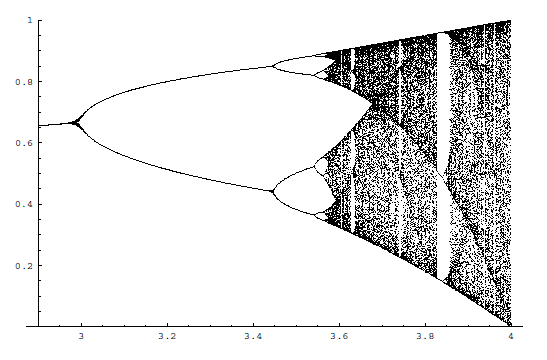
\includegraphics[width=\linewidth]{Immagini/feigenbaum.png}
    
\end{figure}





% ----------------------------------------------------------------------
\subsection*{Definizione di Funzione Caotica}
Una funzione $f: I \to I$ si dice \textbf{caotica} se soddisfa:
\begin{enumerate}
    \item I punti periodici di $f$ sono \textbf{densi} in $I$.
    % (Il resto della definizione prosegue nella pagina successiva degli appunti)

    
    \item $f$ è \textbf{transitiva}: $\forall U_1, U_2 \subset I$, $\exists X_0 \in U_1$ e $m > 0$ tale che:
    $$ f^m(X_0) \in U_2 $$
    \textit{(La mappa esplora prima o poi tutto lo spazio delle fasi).}
    
    \begin{center}
    \begin{tikzpicture}[scale=1.5]
        \draw[thick] (0,0) -- (4,0);
        \node[above] at (2, 0.2) {$I$};
        
        % Intervallo U1
        \draw[thick] (0.5, -0.2) -- (0.5, 0.2);
        \draw[thick] (1.5, -0.2) -- (1.5, 0.2);
    % Parentesi
        \node[below] at (0.8, -0.2) {$U_1$};
        \filldraw[red] (1.2, 0) circle (1pt) node[below, black] {$X_0$};
        
        % Intervallo U2
        \draw[thick] (2.5, -0.2) -- (2.5, 0.2);
        \draw[thick] (3.5, -0.2) -- (3.5, 0.2);
      % Parentesi
        \node[below] at (3, -0.2) {$U_2$};
        \filldraw[red] (2.8, 0) circle (1pt);
        
        % Freccia
        \draw[->, red, thick, bend right=40] (1.2, -0.1) to node[below, black] {$f^m(X_0)$} (2.8, -0.1);
    \end{tikzpicture}
    \end{center}

    \item $f$ è \textbf{sensibile alle condizioni iniziali}: $\exists \beta > 0$ tale che $\forall X_0 \in U \subset I$, $\exists Y_0 \in U$ e $m > 0$ tale che:
    $$ |f^m(X_0) - f^m(Y_0)| > \beta $$
    \textit{(Due traiettorie vicine si separano irrimediabilmente).}
    
    \begin{center}
    \begin{tikzpicture}[scale=1.5]
        \draw[thick] (0,0) -- (5,0);
        
        % Intervallo U
        \draw[thick] (1.5, -0.2) -- (1.5, 0.2);
        \draw[thick] (2.5, -0.2) -- (2.5, 0.2);
        \node[above] at (2, 0.2) {$U$};
        
        % Punti iniziali
        \filldraw[red] (2, 0) circle (1pt) node[below, black] {$X_0$};
        \filldraw[blue] (2.3, 0) circle (1pt) node[below, black] {$Y_0$};
        
        % Punti finali
        \filldraw[red] (1, 0) circle (1pt) node[above, text=red] {$f^m(X_0)$};
        \filldraw[blue] (4.0, 0) circle (1pt) node[above, text=blue] {$f^m(Y_0)$};
        
    \end{tikzpicture}
    \end{center}
\end{enumerate}

\textbf{Commenti sulla Definizione di Mappa Caotica:}
\begin{enumerate}
    \item \textbf{Dimensione:} Questa definizione è generale e vale per sistemi a $m$-dimensioni.
    \item \textbf{Limiti Visivi:} A causa della geometria semplice a $1$ dimensione, alcuni comportamenti sembrano graficamente uguali.
    \item \textbf{Generalità:} Il concetto ha a che vedere con mappe su insiemi; per equazioni differenziali complicate, queste proprietà topologiche sono scritte in modo diverso.
\end{enumerate}


% ----------------------------------------------------------------------
\subsection*{Analisi Geometrica del Caos per la Mappa Logistica ($\lambda = 4$)}

Prendiamo la mappa logistica nel caso limite $\lambda = 4$:
$$ f_4(x) = 4x(1 - x) $$
Valutiamo i punti notevoli della funzione nel dominio $I = [0; 1]$:
\begin{itemize}
    \item \textbf{Vertice} (Punto di MAX): $f_4\left(\frac{1}{2}\right) = 1$ \quad (dove la derivata $f_4'\left(\frac{1}{2}\right) = 0$)
    \item \textbf{Estremi}: $f_4(0) = 0$ e $f_4(1) = 0$
\end{itemize}

Questo significa che la funzione prende la prima metà del dominio $[0; \frac{1}{2}]$ e la espande coprendo l'intero dominio $I$. Fa lo stesso con la seconda metà $[\frac{1}{2}; 1]$.
Quindi possiamo scrivere:
$$ f_4\left( \left[0; \frac{1}{2}\right] \right) = I \quad \text{e} \quad f_4\left( \left[\frac{1}{2}; 1\right] \right) = I $$

Siccome l'immagine di entrambe le metà è l'intero $I$, devono esistere due punti che chiamiamo $Y_0$ e $Y_1$, con $Y_0 \in \left[0; \frac{1}{2}\right]$ e $Y_1 \in \left[\frac{1}{2}; 1\right]$, tali per cui la funzione valga esattamente la metà del codominio:
$$ f_4(Y_0) = f_4(Y_1) = \frac{1}{2} $$

\begin{center}

\begin{tikzpicture}[>=latex, line width=0.8pt]

    % --- Segmento di sinistra [0, 1/2] ---
    \draw (0,0) -- (1.5,0);
    % Ticks e etichette
    \draw (0,0.2) -- (0,-0.2) node[below] {$0$};
    \draw (1.5,0.2) -- (1.5,-0.2) node[below] {$\frac{1}{2}$};

    % --- Freccia curva centrale ---
    \draw[->] (2,0.3) to[out=45, in=135] (3.5,0.3);

    % --- Segmento di destra [0, 1] ---
    \begin{scope}[xshift=4cm]
        \draw (0,0) -- (3,0);
        % Ticks e etichette
        \draw (0,0.2) -- (0,-0.2) node[below] {$0$};
        \draw (1.5,0.2) -- (1.5,-0.2) node[below] {$\frac{1}{2}$};
        \draw (3,0.2) -- (3,-0.2) node[below] {$1$};
    \end{scope}

\end{tikzpicture}
\end{center}

Cosa succede se iteriamo la funzione per studiare $f_4^2$? 
Sappiamo che $f_4\left(\frac{1}{2}\right) = 1$. Applicando $f_4$ ai punti appena trovati:
$$ f_4^2(Y_0) = f_4\left(\frac{1}{2}\right) = 1 \quad \text{e} \quad f_4^2(Y_1) = f_4\left(\frac{1}{2}\right) = 1 $$

Il dominio originario $I$ ora risulta diviso in 4 sotto-intervalli e ciascuno di essi viene mappato dall'iterata seconda su $I$:
\begin{align*}
    f_4^2([0; Y_0]) &= I & f_4^2\left(\left[Y_0; \frac{1}{2}\right]\right) &= I \\
    f_4^2\left(\left[\frac{1}{2}; Y_1\right]\right) &= I & f_4^2([Y_1; 1]) &= I
\end{align*}

\textbf{Regola Generale}\\
La funzione iterata $m$-esima $f_4^m$ manda $2^m$ sotto-intervalli interi nello spazio $I$. \\
(La mappa prende $I$, lo spezza, lo stira e lo rimanda interamente in $I$).


Analizzando graficamente l'intersezione con la bisettrice $y = x$ (che ci indica i punti fissi):

\vspace{1em}
% Dichiarazione funzioni per TikZ per fare iterazioni matematicamente corrette
\tikzset{declare function={
    f(\x) = 4*\x*(1-\x);
    f2(\x) = f(f(\x));
    f3(\x) = f2(f(\x));
}}

\begin{minipage}{0.32\textwidth}
    \centering
    \textbf{$f_4$}\\
    1 cupola, interseca $x$ in 2 punti fissi.
    \vspace{0.5cm}
    
    \begin{tikzpicture}[scale=2.5]
        \draw[thick] (0,0) rectangle (1,1);
        \draw[red, thick] (0,0) -- (1,1);
        \draw[thick, domain=0:1, samples=100] plot (\x, {f(\x)});
        \draw (0.5, 0.05) -- (0.5, -0.05) node[below] {$\frac{1}{2}$};
    \end{tikzpicture}
\end{minipage}
\hfill
\begin{minipage}{0.32\textwidth}
    \centering
    \textbf{$f_4^2$}\\
    2 cupole, interseca $x$ in 4 pt. fissi: 2 originali e 2 periodici di periodo 2.
    \vspace{0.5cm}
    
    \begin{tikzpicture}[scale=2.5]
        \draw[thick] (0,0) rectangle (1,1);
        \draw[red, thick] (0,0) -- (1,1);
        \draw[thick, domain=0:1, samples=200] plot (\x, {f2(\x)});
        
        % Cerchi blu sui punti di periodo 2 (intersezioni che non sono dell'iterata 1)
        \draw[blue, thick] (0.345, 0.345) circle (1.5pt); % approssimazione per il disegno
        \draw[blue, thick] (0.905, 0.905) circle (1.5pt);
    \end{tikzpicture}
\end{minipage}
\hfill
\begin{minipage}{0.32\textwidth}
    \centering
    \textbf{$f_4^3$}\\
    4 cupole, interseca $x$ in 8 pt. fissi: 2 di $f$ e 6 di 3-cicli.
    \vspace{0.5cm}
    
    \begin{tikzpicture}[scale=2.5]
        \draw[thick] (0,0) rectangle (1,1);
        \draw[red, thick] (0,0) -- (1,1);
        \draw[thick, domain=0:1, samples=400] plot (\x, {f3(\x)});
    \end{tikzpicture}
\end{minipage}

\vspace{1.5em}
Per un certo parametro $\mu$ (quando entriamo nel regime caotico) il grafico dell'iterata presenterà un'infinita di oscillazioni tra 0 e 1, generando una nuvola di punti fissi.

\textit{(Se $\frac{m}{k} \in \mathbb{N}$ i cicli di ordine inferiore sono contenuti in quelli di ordine superiore).}

% ----------------------------------------------------------------------
\subsection{La Mappa a Tenda}

Per dimostrare la caoticità della mappa logistica (in $\lambda = 4$) cerchiamo di legare 2 mappe diverse e vediamo se il comportamento è analogo.

Mappa a tenda $T: [0, 1] \to [0, 1]$:
$$ T(x) = \begin{cases} 
2x & \text{se } 0 \leq x \leq \frac{1}{2} \\ 
-2x + 2 & \text{se } \frac{1}{2} \leq x \leq 1 
\end{cases} $$

\begin{minipage}{0.55\textwidth}
    \textbf{Punti Fissi} ($T(x) = x$):
    \begin{itemize}
        \item Per $x \in \left[0; \frac{1}{2}\right]$: \quad $2x = x \implies X^* = 0$
        \item Per $x \in \left[\frac{1}{2}; 1\right]$: \quad $-2x + 2 = x \implies X^* = \frac{2}{3}$
    \end{itemize}
\end{minipage}
\begin{minipage}{0.4\textwidth}
    \begin{center}
    \begin{tikzpicture}[scale=3]
        \draw[thick] (0,0) rectangle (1,1);
        \draw[red, thick] (0,0) -- (1,1);
        \draw[thick] (0,0) -- (0.5,1) -- (1,0);
        
        \draw (0, 0) node[below left] {$0$};
        \draw (0.5, 0.03) -- (0.5, -0.03) node[below] {$\frac{1}{2}$};
        \draw (1, 0) node[below right] {$1$};
        
        \filldraw[blue] (0,0) circle (0.5pt);
        \filldraw[blue] (0.666, 0.666) circle (0.5pt) node[right, black] {$\frac{2}{3}$};
        
        \draw[dashed, thin] (0.5, 0) -- (0.5, 1);
    \end{tikzpicture}
    \end{center}
\end{minipage}

\textbf{Iterata Seconda}: $T^2(x) = T(T(x))$
$$ T^2(x) = 
\begin{cases}
2(2x) & \text{se } 0 \le x \le \frac{1}{4} \quad (\text{perchè } T(x) \le \frac{1}{2}) \\
2 - 2(2x) & \text{se } \frac{1}{4} \le x \le \frac{1}{2} \quad (\text{perchè } T(x) \ge \frac{1}{2}) \\
2 - 2(2-2x) & \text{se } \frac{1}{2} \le x \le \frac{3}{4} \quad (\text{perchè } T(x) \ge \frac{1}{2}) \\
2(2-2x) & \text{se } \frac{3}{4} \le x \le 1 \quad (\text{perchè } T(x) \le \frac{1}{2})
\end{cases}
\quad = \quad
\begin{cases}
4x & 0 \leq x \leq \frac{1}{4} \\
2 - 4x & \frac{1}{4} \leq x \leq \frac{1}{2} \\
-2 + 4x & \frac{1}{2} \leq x \leq \frac{3}{4} \\
4 - 4x & \frac{3}{4} \leq x \leq 1
\end{cases} $$

\textbf{Punti Fissi / Periodici} per $T^2$:
\begin{minipage}{0.3\textwidth}
    \begin{center}
    \begin{tikzpicture}[scale=3]
        \draw[thick] (0,0) rectangle (1,1);
        \draw[red, thick] (0,0) -- (1,1);
        \draw[thick] (0,0) -- (0.25,1) -- (0.5,0) -- (0.75,1) -- (1,0);
        
        \filldraw[blue] (0,0) circle (0.5pt);
        \filldraw[blue] (0.4, 0.4) circle (0.5pt); % 2/5
        \filldraw[blue] (0.666, 0.666) circle (0.5pt); % 2/3
        \filldraw[blue] (0.8, 0.8) circle (0.5pt); % 4/5
    \end{tikzpicture}
    \end{center}
\end{minipage}
\begin{minipage}{0.45\textwidth}
    \begin{itemize}
        \item $4x = x \implies X^* = 0$
        \item $2 - 4x = x \implies \mathbf{x^* = \frac{2}{5}}$
        \item $-2 + 4x = x \implies x^* = \frac{2}{3}$
        \item $4 - 4x = x \implies \mathbf{x^* = \frac{4}{5}}$
    \end{itemize}
    \vspace{0.5cm}
    I valori $x^* = \frac{2}{5}$ e $x^* = \frac{4}{5}$ sono \\  \textcolor{green!60!black}{\textbf{Punti periodici di periodo 2}}.
\end{minipage}

\vspace{1em}
In generale, $T^m$ ha $2^m$ punti fissi, poiché ogni passo fa cambiare la retta di un fattore 2.
\\
\textbf{Teorema}
La mappa a tenda $T$ è \textbf{caotica}.

\begin{enumerate}

\item \textbf{ Punti periodici densi:} \\
$T^m$ mappa ogni piccolo intervallo $\left[\frac{k}{2^m}; \frac{k+1}{2^m}\right]$ in tutto $I = [0; 1]$.
Graficamente $T^m$ interseca la diagonale esattamente 1 volta in ogni intervallo.
Quindi ogni $\left[\frac{k}{2^m}; \frac{k+1}{2^m}\right]$ contiene un punto periodico per $T$.
Poiché la larghezza dell'intervallo $\to 0$ quando $m \to \infty$, i punti periodici sono densi.

\vspace{0.5em}
\begin{center}
\begin{tikzpicture}[scale=3]
    \draw[thick] (0,0) rectangle (1,1);
    \draw[red, thick] (0,0) -- (1,1);
    
    % Mappa T^3 (8 picchi)
    \draw[thick, green!50!black] (0,0) -- (1/8,1) -- (2/8,0) -- (3/8,1) -- (4/8,0) -- (5/8,1) -- (6/8,0) -- (7/8,1) -- (1,0);
    
    % Linee tratteggiate per mostrare i sottointervalli
    \foreach \x in {1,2,3,4,5,6,7} {
        \draw[dashed, thin, gray] (\x/8, -0.1) -- (\x/8, 1.1);
    }
\end{tikzpicture}
\end{center}


    \item \textbf{Transitività:} \\
    Prendo 2 intorni $U_1, U_2$. Per $m$ sufficientemente grande, $U_1$ contiene un intervallo $\left[ \frac{k}{2^m}; \frac{k+1}{2^m} \right]$.
    Siccome $T^m$ manda tutto questo intervallo in $I = [0; 1]$, esisterà sicuramente al suo interno un punto che viene mandato a finire dentro $U_2$.
    
    \begin{center}
    \begin{tikzpicture}[scale=1.5]
        \draw[thick] (0,0) -- (3,0);
        \draw[thick] (0.5, -0.1) -- (0.5, 0.1);
        \draw[thick] (1.5, -0.1) -- (1.5, 0.1);
        \node[below] at (1, -0.1) {$U_1$};
                
        \draw[thick] (2.0, -0.1) -- (2.0, 0.1);
        \draw[thick] (2.8, -0.1) -- (2.8, 0.1);
        \node[below] at (2.4, -0.1) {$U_2$};
        
    \end{tikzpicture}
    \end{center}

    \item \textbf{Dipendenza (sensibilità) dai dati iniziali:} \\
    Scelgo un punto iniziale $X_0 \in U$. Trovo l'intervallo $\left[ \frac{k}{2^m}; \frac{k+1}{2^m} \right]$ contenuto in $U$ che contiene $X_0$.
    Poiché questo viene espanso a tutto $I = [0; 1]$, esisterà sicuramente in $U$ un punto $Y_0$ la cui iterata dista da quella di $X_0$ di almeno metà dell'intero dominio.
    Scegliamo la costante $\beta = \frac{1}{2}$.
    $$ \exists Y_0 \in U \text{ tale che } |T^m(Y_0) - T^m(X_0)| \geq \frac{1}{2} = \beta $$
\end{enumerate}
$\implies T$ è caotica. 

% ----------------------------------------------------------------------


\subsection{Sistemi Coniugati e Caos nella Mappa Logistica}

Consideriamo 2 sistemi dinamici discreti definiti su 2 insiemi diversi:
$$ f: I \to I \quad ; \quad g: J \to J $$

\begin{definizione}[Mappe Coniugate]
Le funzioni $f$ e $g$ sono \textbf{coniugate} se esiste una funzione $h: I \to J$ che sia un \emph{omeomorfismo} (funzione continua, biunivoca con inversa continua) tale per cui il diagramma commuta:
$$ h \circ f = g \circ h $$
\end{definizione}

\begin{minipage}{0.6\textwidth}
    La funzione $h$ porta orbite di $f$ in $g$:
    $$ h(f^m(x)) = g^m(h(x)) $$
    Visivamente la coniugazione porta punti fissi in punti fissi e sistemi caotici in sistemi caotici.
\end{minipage}
\begin{minipage}{0.35\textwidth}
    \begin{center}
    \begin{tikzpicture}[node distance=1.5cm, auto]
        \node (I1) {$I$};
        \node (I2)[right of=I1] {$I$};
        \node (J1) [below of=I1] {$J$};
        \node (J2) [below of=I2] {$J$};
        
        \draw[->, thick] (I1) to node {$f$} (I2);
        \draw[->, thick] (I1) to node[swap] {$h$} (J1);
        \draw[->, thick] (I2) to node {$h$} (J2);
        \draw[->, thick] (J1) to node[swap] {$g$} (J2);
        
        % Diagramma per iterate
        \begin{scope}[yshift=-2.5cm]
            \node (I1) {$I$};
            \node (I2) [right of=I1] {$I$};
            \node (Idots)[right of=I2] {$\dots$};
            \node (Im) [right of=Idots] {$I$};
            \node (J1) [below of=I1] {$J$};
            \node (J2)[below of=I2] {$J$};
            \node (Jdots) [right of=J2] {$\dots$};
            \node (Jm) [below of=Im] {$J$};
            
            \draw[->, thick] (I1) to node {$f$} (I2);
            \draw[->, thick] (I2) to (Idots);
            \draw[->, thick] (Idots) to (Im);
            
            \draw[->, thick] (I1) to node[swap] {$h$} (J1);
            \draw[->, thick] (I2) to node {$h$} (J2);
            \draw[->, thick] (Im) to node {$h$} (Jm);
            
            \draw[->, thick] (J1) to node[swap] {$g$} (J2);
            \draw[->, thick] (J2) to (Jdots);
            \draw[->, thick] (Jdots) to (Jm);
        \end{scope}
    \end{tikzpicture}
    \end{center}
\end{minipage}

\vspace{1em}
\textbf{Teorema} (Conservazione del caos)
Siano $f: I \to I$ e $g: J \to J$ (con $I, J$ intervalli finiti) coniugate tramite $h: I \to J$. \\
Allora: se $f$ è caotica $\implies g$ è caotica.


\begin{dimostrazione}
Prendiamo $U \subset J$ e consideriamo la retro-immagine $h^{-1}(U) \subset I$.
\begin{enumerate}
    \item \textbf{Punti periodici densi:} \\
    $f$ è caotica $\implies$ i suoi punti periodici sono densi, posso trovare $x \in h^{-1}(U)$ che sia un punto periodico di periodo $m$ (cioè $f^m(x) = x$).
    Applico la regola della coniugazione all'$m$-esima iterata:
    $$ h(\underbrace{f^m(x)}_{= x}) = g^m(h(x)) \implies h(x) = g^m(h(x)) $$
    Quindi $h(x)$, che sta in $U$, è un punto periodico di periodo $m$ che sta in $g$. I punti periodici di $g$ sono densi.
    
    \item \textbf{Transitività:} \\
    Siano $U, V \subset J$. Per transitività di $f$, $\exists x \in h^{-1}(U)$ e $\exists m$ tale che $f^m(x) \in h^{-1}(V)$.
    Ma se $x \in h^{-1}(U)$ allora $h(x) \in U$.
    Inoltre $g^m(h(x)) = h(f^m(x)) \in V$.
    Partendo da $h(x) \in U$, dopo $m$ passi cado in $V \implies g$ è transitiva.

    \item \textbf{Sensibilità:} \\
    Supponiamo $I = [\alpha_1, \alpha_2]$ e sia $\beta < \alpha_2 - \alpha_1$ la costante di sensibilità di $f$.
    Consideriamo $\forall x \in [\alpha_1, \alpha_2 - \beta]$ la distanza $|h(x+\beta) - h(x)|$.
    Essendo $h$ continua, questa è una funzione continua su un intervallo chiuso e limitato ed è strettamente positiva. Per il Teorema di Weierstrass, essa ha un valore minimo assoluto che chiamiamo $\beta' > 0$.
    Quindi $h$ prende intervalli di lunghezza $\beta$ in $I$ e li manda in intervalli di lunghezza almeno $\beta'$ in $J$. 
    Prendo $\beta'$ come costante di sensibilità per $g$.
\end{enumerate}
\end{dimostrazione}

% ----------------------------------------------------------------------
\subsubsection*{Semi-coniugazione}
Non è strettamente necessario che $h$ sia biunivoca ("1 a 1"). Può essere al più "N a 1", purché soddisfi la proprietà di commutazione $h \circ f = g \circ h$.
Una \emph{semi-coniugazione} manda sistemi caotici in sistemi caotici, ma non preserva il periodo (non mantiene le esatte periodicità).

\textbf{Teorema}: La mappa logistica è caotica]
La mappa logistica $f_4(x) = 4x(1-x)$ è caotica.


\begin{dimostrazione}
Dimostriamo che $f_4$ è semi-coniugata alla mappa a tenda $T$ (che sappiamo già essere caotica). \\
Scegliamo come funzione di traduzione $h: [0; 1] \to [0; 1]$ definita da:
$$ h(x) = \frac{1}{2} (1 - \cos(2\pi x)) $$
Questa funzione è "2 a 1" su $[0; 1]$ (tranne che in $x = \frac{1}{2}$). Quindi è una semi-coniugazione.
Verifichiamo la commutazione calcolando $h(T(x))$.
Ricordando che $T(x) = 2x$ per $x \leq \frac{1}{2}$ e $T(x) = 2-2x$ per $x \geq \frac{1}{2}$, inserendo $T(x)$ nell'argomento del coseno otteniamo:
$$
h(T(x)) = 
\begin{cases}
    \frac{1}{2} (1 - \cos(2\pi \cdot 2x)) = \frac{1}{2} (1 - \cos(4\pi x)) & 0 \leq x \leq \frac{1}{2} \\
    \frac{1}{2} (1 - \cos(2\pi(2 - 2x))) = \frac{1}{2} (1 - \cos(4\pi - 4\pi x)) & \frac{1}{2} \leq x \leq 1
\end{cases}
$$
Siccome il coseno è una funzione pari e periodica (di periodo $2\pi$, quindi anche $4\pi$), nel secondo ramo l'argomento diventa equivalente a $4\pi x$. La funzione è unica per tutto il dominio:
$$ h(T(x)) = \frac{1}{2} (1 - \cos(4\pi x)) $$

Usiamo ora la formula di duplicazione del coseno ($\cos(2\theta) = 2\cos^2\theta - 1$) scegliendo $\theta = 2\pi x$:
\begin{align*}
    h(T(x)) &= \frac{1}{2} - \frac{1}{2} \left[ 2\cos^2(2\pi x) - 1 \right] \\
    &= \frac{1}{2} - \cos^2(2\pi x) + \frac{1}{2} \\
    &= 1 - \cos^2(2\pi x) 
\end{align*}

Con un intelligente artificio algebrico (una scomposizione analoga a $(a^2-b^2) = (a-b)(a+b)$ modificata ad hoc), possiamo riscrivere questa espressione come:
$$ h(T(x)) = 4 \left( \frac{1}{2} - \frac{1}{2}\cos(2\pi x) \right) \left( \frac{1}{2} + \frac{1}{2}\cos(2\pi x) \right) $$

Osserviamo i termini nelle parentesi:
\begin{itemize}
    \item Il \textbf{primo termine} è esattamente la definizione di $h(x)$.
    \item Il \textbf{secondo termine} può essere scritto come $1 - \left( \frac{1}{2} - \frac{1}{2}\cos(2\pi x) \right)$, ovvero $1 - h(x)$.
\end{itemize}

Quindi sostituendo otteniamo:
$$ h(T(x)) = 4 \cdot h(x) \cdot (1 - h(x)) $$
Che è esattamente la definizione della mappa logistica $f_4$ valutata nel punto $h(x)$:
$$ h(T(x)) = f_4(h(x)) $$

Avendo dimostrato che $h \circ T = f_4 \circ h$, per il teorema precedente (esteso alle semi-coniugazioni) la mappa logistica $f_4$ è \textbf{caotica}. \qed
\end{dimostrazione}

% ----------------------------------------------------------------------

\section{L'Esponente di Lyapunov}

Rappresenta una \textbf{misura qualitativa} del caos.
Ci chiediamo: \emph{il tasso di repulsione tra 2 traiettorie partite molto vicine è di tipo esponenziale?} Se sì, il sistema manifesta estrema sensibilità alle condizioni iniziali.

Prendiamo un punto iniziale $X_0$ e un punto infinitesimamente vicino $X_0 + \epsilon$.
Sottoponiamoli alla stessa evoluzione $X_{m+1} = f(X_m)$.

\begin{definizione}
L'esponente di Lyapunov $\lambda$ si definisce come:
$$ \lambda = \lim_{\substack{N \to \infty \\ \epsilon \to 0}} \frac{1}{N} \log \frac{|f^N(X_0 + \epsilon) - f^N(X_0)|}{\epsilon} $$
\end{definizione}

\textbf{Significato:}
L'idea alla base è che le due traiettorie si separano come $e^{\lambda N}$. Ovvero:
$$ e^{\lambda N} \sim \lim_{\epsilon \to 0} \frac{|f^N(X_0 + \epsilon) - f^N(X_0)|}{\epsilon} $$
Se $\mathbf{\lambda > 0}$, da punti molto vicini mi distacco esponenzialmente (\textbf{Caos}).

Osservando il termine per $\epsilon \to 0$ nel limite, riconosciamo la definizione formale di \textbf{derivata} della funzione iterata $f^N$ valutata in $X_0$.
Possiamo quindi riscrivere il tutto nella forma pratica:
$$ \lambda = \lim_{N \to \infty} \frac{1}{N} \log \left| \left. \frac{df^N}{dx} \right|_{X_0} \right| $$

Ovvero in notazione più compatta per valutare la sensibilità:
$$ \lambda = \lim_{N \to \infty} \frac{1}{N} \log \left| \left. \frac{df^N}{dx} \right|_{x_0} \right| $$



\subsection*{Derivazione Esponente Lyapunov ($\lambda$)}
Osserviamo come varia la derivata di una funzione composta (iterata) per definire $\lambda$ in modo calcolabile.
Usando la regola della catena (Chain Rule):
$$ (f^N)'(x_0) = \left[ f(f^{N-1}(x_0)) \right]' = f'(f^{N-1}(x_0)) \cdot (f^{N-1})'(x_0) $$

Iterando il processo $N$ volte si ottiene la moltiplicazione delle derivate valutate nei vari punti dell'orbita:
$$ (f^N)'(x_0) = \underbrace{f'(f^{N-1}(x_0))}_{x_{N-1}} \cdot \underbrace{f'(f^{N-2}(x_0))}_{x_{N-2}} \cdot \dots \cdot \underbrace{f'(f(x_0))}_{x_1} \cdot \underbrace{f'(x_0)}_{x_0} $$

In forma compatta:
$$ (f^N)'(x_0) = \prod_{i=0}^{N-1} f'(x_i) $$

Dunque, sostituendo nella definizione originaria di limite:
$$ \lambda = \lim_{N \to \infty} \frac{1}{N} \log |(f^N)'(x_0)| = \lim_{N \to \infty} \frac{1}{N} \log \left| \prod_{i=0}^{N-1} f'(x_i) \right| $$

Per le proprietà dei logaritmi (il logaritmo di un prodotto è la somma dei logaritmi):
$$ \lambda = \lim_{N \to \infty} \frac{1}{N} \sum_{i=0}^{N-1} \log |f'(x_i)| $$

% ----------------------------------------------------------------------
\section{Approfondimenti sul Caos e Dinamica Simbolica}

\subsection{Stabilità dei\texorpdfstring{$k$-cicli}{k cicli}}
\textbf{Condizioni di stabilità:} Ricordando che un punto fisso $X_0$ è stabile se $|f'(X_0)| < 1$, similmente un $k$-ciclo di periodo $k$ è stabile se la derivata dell'iterata $k$-esima è minore di uno:
$$ |(f^k)'(X_0)| < 1 $$

In termini logaritmici, questo equivale a dire:
$$ \log |(f^k)'(X_0)| < \log(1) = 0 $$

\subsubsection*{Relazione tra $\lambda$ e $k$-cicli}
Per un'orbita che appartiene a un $k$-ciclo, il limite della media per $N \to \infty$ si riduce alla media calcolata solo sui $k$ punti del ciclo:
$$ \lambda = \frac{1}{k} \sum_{i=0}^{k-1} \log |f'(x_i)| $$

\begin{dimostrazione}[Verifica sui limiti delle successioni periodiche]
Si può verificare considerando la scomposizione della sommatoria. Sia $p$ il periodo (o $k$). Possiamo dividere l'intero $N$ in blocchi di lunghezza $p$ più un eventuale resto:
$$ \bar{x} = \frac{1}{N} \sum_{i=1}^N x_i = \frac{1}{N} \left( \left\lfloor \frac{N}{p} \right\rfloor \sum_{i=1}^p x_i + \sum_{j=1}^{N \bmod p} x_j \right) $$
Moltiplicando e dividendo il primo termine per $p$:
$$ = \frac{\lfloor N/p \rfloor}{\lfloor N/p \rfloor p + \text{resto}} \cdot p \left( \frac{1}{p} \sum_{i=1}^p x_i \right) + \frac{1}{N} \sum_{j=1}^{N \bmod p} x_j $$
Facendo tendere $N \to \infty$, il termine con il resto diviso per $N$ tende a zero. I termini che sopravvivono sono quelli ripetuti del ciclo:
$$ \xrightarrow{N \to \infty} \frac{1}{p} \sum_{i=1}^p x_i $$
\end{dimostrazione}

Tornando al nostro esponente di Lyapunov per l'orbita periodica, ricordando che $\sum_{i=0}^{k-1} \log|f'(x_i)| = \log \left| \prod_{i=0}^{k-1} f'(x_i) \right| = \log|(f^k)'(X_0)|$:
$$ \lambda = \frac{1}{k} \log |(f^k)'(X_0)| < 0 $$

Dato che per la stabilità deve valere $|(f^k)'(X_0)| < 1$, ne consegue che \textbf{$\forall$ ciclo stabile, si ha $\lambda < 0$}.

% ----------------------------------------------------------------------
\subsection{Cicli Super-Stabili}

Un ciclo è detto \textbf{SUPER-STABILE} quando la derivata dell'iterata valutata nel punto è esattamente nulla:
$$ |(f^k)'(X_0)| = 0 $$

In questo caso l'esponente di Lyapunov diverge a meno infinito:
$$ \lambda = \frac{1}{k} \log(0) = -\infty $$

% ----------------------------------------------------------------------
\subsection{Mappa a Tenda (Lyapunov)}

Si prenda la mappa a tenda generalizzata con parametro $r$:
$$ T(x) = \begin{cases} 
2rx & 0 \leq x \leq \frac{1}{2} \\ 
2r(1-x) & \frac{1}{2} \leq x \leq 1 
\end{cases} $$

Il modulo della derivata di questa funzione è costante quasi ovunque (tranne nel punto $x = \frac{1}{2}$ dove non è definita):
$$ |T'(x)| = 2r \quad \forall x \in [0; 1], \ x \neq \frac{1}{2} $$

Calcoliamo l'esponente di Lyapunov $\lambda$:
$$ \lambda = \lim_{N \to \infty} \frac{1}{N} \sum_{i=0}^{N-1} \log |T'(x_i)| $$
Poiché il modulo della derivata è sempre $2r$:
$$ \lambda = \lim_{N \to \infty} \frac{1}{N} \sum_{i=0}^{N-1} \log(2r) = \lim_{N \to \infty} \frac{1}{N} \cdot N \log(2r) = \log(2r) $$

\textbf{Conclusioni:}
\begin{itemize}
    \item Se $r > \frac{1}{2}$, allora $\lambda = \log(2r) > \log(1) = 0$.
    \item Quando $\mathbf{\lambda > 0}$, la mappa è \textbf{caotica} e le traiettorie divergono esponenzialmente.
\end{itemize}



% ----------------------------------------------------------------------

\subsection{Mappa Logistica con\texorpdfstring{$\lambda > 4$}{lambda > 4}}

Studiamo il caso $f_\lambda(x) = \lambda x(1-x)$ con $\lambda > 4$. \\
In questo scenario, il valore massimo della funzione supera $1$. L'intervallo $I =[0, 1]$ \textbf{non è più invariante}.

\begin{minipage}{0.45\textwidth}
    \begin{center}
    \begin{tikzpicture}[scale=3.5]
        % Assi e Box
        \draw[thick] (0,0) rectangle (1,1);
        \draw[black, thick] (0,0) -- (1,1); % Bisettrice
        
        % Parabola (e.g., lambda = 4.5)
        \draw[blue, thick, domain=0:1, samples=100] plot (\x, {4.5*\x*(1-\x)});
        
        % A_0
        \draw[dashed, thin, red] (0.275, 1) -- (0.275, 0);
        \draw[dashed, thin, red] (0.725, 1) -- (0.725, 0);
        
        % Asse di simmetria
        \draw[dashed, thin, gray] (0.5, 0) -- (0.5, 1.125) node[above, black] {$x=\frac{1}{2}$};
        
        % Evidenziazione A_0
        \draw[red, thick, |-|] (0.275, -0.05) -- (0.725, -0.05) node[midway, below] {$A_0$};
        \draw[green!60!black, thick] (0, -0.05) -- (0.275, -0.05);
        \draw[green!60!black, thick] (0.725, -0.05) -- (1, -0.05);
        
        % Labels
        \node[left] at (0,1) {$1$};
        \node[below left] at (0,0) {$0$};
        \node[below right] at (1,0) {$1$};
    \end{tikzpicture}
    \end{center}
\end{minipage}
\begin{minipage}{0.5\textwidth}
    \begin{itemize}
        \item Esiste un intervallo centrale $A_0$ tale che $\forall x \in A_0$, si ha $f_\lambda(x) > 1$.
        \item Le orbite dei punti in $A_0$ "scappano" verso $-\infty$.
        \item Gli estremi di $A_0$ (dove $f_\lambda(x) = 1$) finiscono in $0$ al passo successivo.
    \end{itemize}
\end{minipage}

% ----------------------------------------------------------------------
\subsection{Costruzione dell'Insieme Invariante\texorpdfstring{$\Lambda$}{Lambda}}

Vogliamo identificare l'insieme $\Lambda$ dei punti le cui orbite non escono mai da $I$:
$$ \Lambda = \{ \text{punti } x \in I : f^n(x) \in I \quad \forall n \} $$

\begin{minipage}{0.45\textwidth}
    \begin{center}
    \begin{tikzpicture}[scale=3.5]
        % Assi e Box
        \draw[thick] (0,0) rectangle (1,1);
        \draw[black, thick] (0,0) -- (1,1);
        
        % Parabola
        \draw[blue, thick, domain=0:1, samples=100] plot (\x, {4.5*\x*(1-\x)});
        
        % A_0
        \draw[dashed, thin, red] (0.3, 1) -- (0.3, 0);
        \draw[dashed, thin, red] (0.7, 1) -- (0.7, 0);
        \draw[red, thick, |-|] (0.275, -0.05) -- (0.725, -0.05) node[midway, below] {$A_0$};
        
        % Pallini verdi all'intersezione tra la retta e le linee rosse
        \fill[green!50!black] (0.30, 0.286) circle (0.7pt);
        \fill[green!50!black] (0.700, 0.707) circle (0.7pt);
        
        % Orizzontali per A_1
        \draw[dashed, thin, cyan] (0.1, 0.275) -- (0.95, 0.275);
        \draw[dashed, thin, cyan] (0.27, 0.725) -- (0.75, 0.725);
        
        % A_1 (proiezioni)
        \draw[dashed, thin, cyan] (0.065, 0.275) -- (0.065, 0);
        \draw[dashed, thin, cyan] (0.21, 0.725) -- (0.21, 0);
        \draw[dashed, thin, cyan] (0.79, 0.725) -- (0.79, 0);
        \draw[dashed, thin, cyan] (0.935, 0.275) -- (0.935, 0);
        
        \draw[cyan, thick, |-|] (0.065, -0.15) -- (0.21, -0.15) node[midway, below] {$A_1$};
        \draw[cyan, thick, |-|] (0.79, -0.15) -- (0.935, -0.15) node[midway, below] {$A_1$};
        
        % Labels
        \node[left] at (0,1) {$1$};
        \node[below left] at (0,0) {$0$};
        \node[below right] at (1,0) {$1$};
    \end{tikzpicture}
    \end{center}
\end{minipage}
\begin{minipage}{0.5\textwidth}
    \begin{itemize}
        \item $A_0$: intervallo che esce al primo passo.
        \item $A_1$: pre-immagine di $A_0$. È composto da 2 intervalli. Questi vengono mandati negli in \textcolor{green!50!black}{estremi} di $A_0$ e poi in $0$.
        \item $A_2$: composto da 4 intervalli.
        \item $\dots$
        \item $A_N$: composto da $2^N$ intervalli.
    \end{itemize}
\end{minipage}

\vspace{1em}
\begin{tcolorbox}[colback=yellow!5!white,colframe=yellow!60!black]
Sottraendo progressivamente questi intervalli di "fuga" ($I - A_0; I - A_0 - A_1; \dots$), ciò che rimane è l'insieme $\Lambda$, che ha la struttura di un \textbf{Insieme di Cantor}.
\end{tcolorbox}

% ----------------------------------------------------------------------
 \subsection{Dinamica Simbolica e Spazio delle Sequenze}

Per studiare il comportamento dei punti nell'insieme invariante $\Lambda$, si introduce la \textbf{dinamica simbolica}.

\subsubsection*{Funzione Itinerario}
Dato un punto $x \in \Lambda$, la sua orbita rimarrà sempre all'interno dell'unione degli intervalli $I_0 \cup I_1$ (dove $I_0$ è a sinistra di $A_0$ e $I_1$ a destra).
Possiamo quindi associare a ogni punto una \textbf{sequenza infinita} $S(x)$ che ne descrive il percorso:
$$ S(x) = (s_0, s_1, s_2, \dots) $$

Dove l'$i$-esimo elemento è definito come:
$$ s_i = k \iff f_\lambda^i(x) \in I_k \quad \text{con } k \in \{0, 1\} $$

\textbf{Esempi di sequenze:}
\begin{itemize}
    \item $S(0) = (0, 0, 0, \dots) \to$ Orbita del punto fisso in $I_0$.
    \item $S(X^*) = (1, 1, 1, \dots) \to$ Orbita del punto fisso in $I_1$.
    \item $S(1) = (1, 0, 0, \dots) \to$ Il punto 1 (che sta in $I_1$) cade in 0 dopo una iterazione e vi rimane.
\end{itemize}

% ----------------------------------------------------------------------
\subsubsection*{Spazio delle Sequenze $\Sigma$}

Definiamo $\Sigma$ come l'insieme di tutte le possibili sequenze infinite composte da 0 e 1:
$$ \Sigma = \{ S = (s_0, s_1, s_2, \dots) \ : \ s_i \in \{0, 1\} \} $$

% ----------------------------------------------------------------------
\subsubsection*{Metrica nello Spazio $\Sigma$}

Per confrontare 2 sequenze (es. $s$ e $t$) in $\Sigma$, definiamo una \textbf{distanza} $d(s,t)$ che rende $\Sigma$ uno spazio metrico:
$$ d(s, t) = \sum_{i=0}^{\infty} \frac{|s_i - t_i|}{2^i} $$

Questa metrica rispetta le proprietà fondamentali degli spazi metrici:
\begin{enumerate}
    \item \textbf{Positività:} $d(s,t) \geq 0 \quad \text{e} \quad d(s,t) = 0 \iff s = t$
    \item \textbf{Simmetria:} $d(s,t) = d(t,s)$
    \item \textbf{Disuguaglianza Triangolare:} $d(s,u) \leq d(s,t) + d(t,u)$
\end{enumerate}

% ----------------------------------------------------------------------

\subsubsection*{Proprietà e Limiti della Distanza}

\begin{itemize}
    \item \textbf{Distanza Massima:} La distanza massima tra 2 sequenze è 2.
    $$ d(s, t) \leq \sum_{i=0}^{\infty} \frac{1}{2^i} = \frac{1}{1 - \frac{1}{2}} = 2 $$
    
    \item \textbf{Esempio 1:} Distanza tra la sequenza di tutti zero $(\overline{0})$ e tutti uno $(\overline{1})$.
    $$ d((\overline{0}), (\overline{1})) = \sum_{i=0}^{\infty} \frac{1}{2^i} = 2 $$
    
    \item \textbf{Esempio 2:} Distanza tra la sequenza alternata $(\overline{01}) = 0, 1, 0, 1, \dots$ e la sequenza $(\overline{1}) = 1, 1, 1, 1, \dots$ \\
    I termini differiscono solo per gli indici pari ($i = 0, 2, 4, \dots$ dove $s_i=0$ e $t_i=1$). Per gli indici dispari i termini sono uguali ($s_i=1, t_i=1$) e il numeratore è $0$. La somma avviene quindi sui valori pari ($i = 2k$):
    $$ d((\overline{01}), (\overline{1})) = \sum_{k=0}^{\infty} \frac{1}{2^{2k}} = \sum_{k=0}^{\infty} \frac{1}{4^k} = \frac{1}{1 - \frac{1}{4}} = \frac{4}{3} $$
\end{itemize}

\vspace{1.5em}
\textbf{Proposizione sulla vicinanza: }
Due sequenze sono considerate "vicine" se i loro primi termini coincidono.

\begin{enumerate}
    \item \textbf{Proposizione 1:} Se $s_i = t_i$ per $i = 0, \dots, N$, allora $d(s, t) \leq \frac{1}{2^N}$.
    
    \begin{dimostrazione}
    Spezziamo la sommatoria della distanza:
    $$ d(s, t) = \sum_{i=0}^{N} \frac{|s_i - t_i|}{2^i} + \sum_{i=N+1}^{\infty} \frac{|s_i - t_i|}{2^i} $$
    Il primo termine è 0 perché i simboli coincidono. Maggiorando la distanza dei simboli rimanenti con il loro massimo (cioè 1):
    $$ d(s, t) \leq 0 + \frac{1}{2^{N+1}} \sum_{j=0}^{\infty} \frac{1}{2^j} = 0 + \frac{1}{2^{N+1}} \cdot 2 = \frac{1}{2^N} $$
    \end{dimostrazione}
    
    \item \textbf{Proposizione 2:} Se $d(s, t) < \frac{1}{2^N}$, allora le sequenze devono coincidere per i primi $N+1$ termini ($s_j = t_j \ \forall j \leq N$).
    
    \begin{dimostrazione}
    Se così non fosse (altrimenti), esisterebbe almeno un indice $j \leq N$ tale per cui i simboli differiscono. In quel caso avremmo:
    $$ d(s, t) \geq \frac{|s_j - t_j|}{2^j} = \frac{1}{2^j} \geq \frac{1}{2^N} \quad (\text{poiché } j \leq N) $$
    Ma questo contraddice l'ipotesi stretta $d(s,t) < \frac{1}{2^N}$. \qed
    \end{dimostrazione}
\end{enumerate}


\textbf{Teorema (dell'Omeomorfismo)}: \\
La funzione itinerario $S: \Lambda \to \Sigma$ è un \textbf{OMEOMORFISMO} \\
(ovvero è una funzione Continua, Biunivoca, con Inversa Continua).

\begin{dimostrazione}
Per semplicità assumiamo che $\lambda$ sia sufficientemente grande tale che la derivata sia espansiva ovunque nell'insieme di interesse:
$$ |f_\lambda'(x)| > K > 1 \quad \forall x \in I_0 \cup I_1 $$

\textbf{1) INIETTIVITÀ (1 a 1)} \\
Supponiamo per assurdo che 2 punti distinti $x, y \in \Lambda$ abbiano lo stesso itinerario: $S(x) = S(y)$.
\begin{itemize}
    \item Poiché hanno lo stesso itinerario, i loro iterati $f_\lambda^N(x)$ e $f_\lambda^N(y)$ si trovano sempre (per ogni $N$) dallo stesso lato rispetto a $\frac{1}{2}$.
    
    \begin{center}
    \begin{tikzpicture}[scale=2.5]
        \draw[thick] (0,0) rectangle (1,1);
        \draw[black, thick] (0,0) -- (1,1);
        
        % Parabola lambda grande
        \draw[blue, thick, domain=0:1, samples=100] plot (\x, {4.2*\x*(1-\x)});
        
        % Linea mediana 1/2
        \draw[dashed, thin, gray] (0.5, 0) -- (0.5, 1.1) node[above, black] {$\frac{1}{2}$};
        
        % Punti x e y vicini dalla stessa parte
        \draw[red, thick] (0.15, 0) -- (0.15, 0.53);
        \draw[red, thick] (0.18, 0) -- (0.18, 0.62);
        
        % Cerchio per evidenziare i punti
        \draw[blue, thick] (0.165, 0.575) circle (0.1cm);
        
        \node[left] at (0,1) {$1$};
        \node[below left] at (0,0) {$0$};
        \node[below right] at (1,0) {$1$};
    \end{tikzpicture}
    \end{center}
    
    \item Ciò implica che la funzione $f_\lambda^N$ è \textbf{monotona} nell'intervallo tra i 2 punti.
    \item Tuttavia, poiché $|f_\lambda'| > K > 1$, ad ogni iterazione l'intervallo tra $f_\lambda^N(x)$ e $f_\lambda^N(y)$ viene espanso di un fattore $K$.
    \item Crescendo esponenzialmente, la distanza tra gli iterati finirà per superare la lunghezza degli intervalli $I_0$ e $I_1$, portando i punti su lati opposti di $\frac{1}{2}$. Ma ciò contraddice l'ipotesi che abbiano lo stesso itinerario per sempre. Quindi deve essere $\mathbf{x = y}$.
\end{itemize}

\vspace{1em}
\textbf{2) SURIETTIVITÀ} \\
Dobbiamo dimostrare che $\forall$ sequenza $S = (s_0, s_1, s_2, \dots) \in \Sigma$, esiste un punto $x \in \Lambda$ tale che $S(x) = S$.
Si definiscono gli intervalli chiusi annidati:
$$ I_{s_0 \dots s_N} = \{ x \in I : f_\lambda^j(x) \in I_{s_j} \text{ per } j=0, \dots, N \} $$

L'intervallo $I_{s_0 \dots s_N}$ può essere espresso tramite le pre-immagini dei singoli intervalli:
$$ I_{s_0 \dots s_N} = I_{s_0} \cap f_\lambda^{-1}(I_{s_1}) \cap f_\lambda^{-2}(I_{s_2}) \cap \dots \cap f_\lambda^{-N}(I_{s_N}) $$
O in forma ricorsiva:
$$ I_{s_0 \dots s_N} = I_{s_0} \cap f_\lambda^{-1}(I_{s_1 \dots s_N}) $$

\textbf{Proprietà Fondamentali (per induzione):}
\begin{enumerate}
    \item \textbf{Esistenza:} $f_\lambda^{-1}(I_{s_1 \dots s_N})$ è costituito da 2 intervalli disgiunti, uno contenuto in $I_0$ e l'altro in $I_1$. L'intersezione con $I_{s_0}$ ne seleziona \textit{esattamente 1}. Dunque $I_{s_0 \dots s_N}$ è un singolo intervallo non vuoto.
    \item \textbf{Annidamento:} Gli intervalli sono uno dentro l'altro:
    $$ I_{s_0 \dots s_N} \subset I_{s_0 \dots s_{N-1}} $$

    \item \textbf{Limite:} L'intersezione infinita $\bigcap_{N=0}^{\infty} I_{s_0 \dots s_N}$ è non vuota e contiene \textbf{un unico punto} $x \in \Lambda$. Tale punto ha come itinerario esattamente la sequenza desiderata $S(x) = (s_0, s_1, \dots)$.
\end{enumerate}

\vspace{1em}
\textbf{3) CONTINUITÀ} \\
Dimostriamo che la funzione $S: \Lambda \to \Sigma$ è continua utilizzando la definizione $\epsilon - \delta$.
Sia $x \in \Lambda$ con itinerario $S(x) = (s_0, s_1, \dots)$. 
Fissiamo un $\epsilon > 0$ e scegliamo un intero $N$ tale che $\frac{1}{2^N} < \epsilon$.
\begin{itemize}
    \item L'insieme invariante è contenuto nell'unione dei $2^{N+1}$ intervalli disgiunti del tipo $I_{s_0 \dots s_N}$.
    \item Poiché questi intervalli sono separati, possiamo trovare un $\delta > 0$ tale che, se un punto $y \in \Lambda$ dista da $x$ meno di $\delta$ ($|x - y| < \delta$), allora $y$ deve \textit{necessariamente} cadere nello stesso intervallo $I_{s_0 \dots s_N}$ in cui si trova $x$.
    \item Se $x$ e $y$ sono nello stesso intervallo di ordine $N$, significa che le loro prime $N+1$ componenti dell'itinerario coincidono.
    \item Applicando la definizione di distanza nello spazio $\Sigma$:
    $$ d(S(x), S(y)) \leq \sum_{i=N+1}^{\infty} \frac{1}{2^i} = \frac{1}{2^N} < \epsilon $$
\end{itemize}
La funzione $S$ è quindi \textbf{continua}. In modo analogo si dimostra che anche la sua inversa è continua. \qed
\end{dimostrazione}

% ----------------------------------------------------------------------

\subsection{Mappa di Shift}

Per studiare la dinamica simbolica, introduciamo l'operatore di Shift $\sigma$ sullo spazio delle sequenze $\Sigma$:
$$ \sigma: \Sigma \to \Sigma \quad ; \quad \sigma(s_0, s_1, s_2, \dots) = (s_1, s_2, s_3, \dots) $$

Questa mappa \textbf{sposta la sequenza verso sinistra, eliminando il primo simbolo}.

\subsubsection*{Proprietà e Punti Periodici}
Questa mappa $\sigma$ è:
\begin{enumerate}
    \item \textbf{Caotica}
    \item \textbf{Coniugata} a $f_\lambda$  
    \item \textbf{Facile} da manipolare teoricamente.
\end{enumerate}

I punti periodici risultano essere immediati da identificare:
\begin{itemize}
    \item \textbf{Punti Fissi (Periodo 1):} Sono le sequenze costanti.
    $$ (\overline{0}) = (0, 0, 0, \dots) $$
    $$ (\overline{1}) = (1, 1, 1, \dots) $$
    
    \item \textbf{2-Cicli:} Sequenze che si ripetono ogni 2 simboli.
    $$ (\overline{01}) = (0, 1, 0, 1, \dots) $$
    $$ (\overline{10}) = (1, 0, 1, 0, \dots) $$
    
    \item \textbf{N-Cicli:} In generale, ogni sequenza periodica $(\overline{s_0, \dots, s_{N-1}})$ di lunghezza $N$ corrisponde a un'orbita ciclica di periodo $N$.
\end{itemize}

% --- CONTINUAZIONE DALLA SEZIONE "MAPPA DI SHIFT" ---

\vspace{1.5em}
\textbf{Proposizione: }
La mappa di shift $\sigma: \Sigma \to \Sigma$ è \textbf{continua}.

\begin{dimostrazione}
Sia $s = (s_0, s_1, s_2, \dots) \in \Sigma$. Fissiamo un $\epsilon > 0$ e scegliamo un intero $N$ tale che:
$$ \frac{1}{2^N} < \epsilon $$
Poniamo $\delta = \frac{1}{2^{N+1}}$. Consideriamo una sequenza qualsiasi $t = (t_0, t_1, \dots)$ tale che la distanza iniziale sia strettamente minore di $\delta$:
$$ d(s, t) < \delta = \frac{1}{2^{N+1}} $$

Procediamo per passi:
\begin{enumerate}
    \item Dalla definizione di distanza e dalle proposizioni sulla vicinanza dimostrate in precedenza, se $d(s, t) < \frac{1}{2^{N+1}}$, allora i primi $N+2$ termini delle due sequenze devono necessariamente coincidere:
    $$ s_i = t_i \quad \forall i = 0, 1, \dots, N+1 $$
    
    \item Applichiamo lo shift alle due sequenze:
    \begin{align*}
        \sigma(s) &= (s_1, s_2, s_3, \dots) \\
        \sigma(t) &= (t_1, t_2, t_3, \dots)
    \end{align*}
    
    \item Poiché sapevamo che $s_i = t_i$ per $i$ che va da $0$ a $N+1$, le sequenze "shiftate" coincideranno almeno per i loro primi $N+1$ termini (cioè da indice $0$ a $N$ della nuova sequenza).
    
    \item Calcolando la distanza tra le sequenze traslate (usando la proposizione sulla vicinanza per sequenze che coincidono nei primi $N+1$ termini):
    $$ d(\sigma(s), \sigma(t)) \leq \frac{1}{2^N} < \epsilon $$
\end{enumerate}
Avendo verificato che $\forall \epsilon > 0, \exists \delta > 0$ tale che se $d(s,t)<\delta \implies d(\sigma(s),\sigma(t))<\epsilon$, la mappa $\sigma$ è dunque \textbf{continua}. \qed
\end{dimostrazione}

% ----------------------------------------------------------------------
\subsection{Teorema di Coniugazione tra\texorpdfstring{$f_\lambda$ e $\sigma$}{f lambda e sigma}}

La funzione itinerario $S: \Lambda \to \Sigma$ è una \textbf{coniugazione (topologica)} tra la mappa logistica $f_\lambda$ (limitata all'insieme invariante $\Lambda$) e la mappa di shift $\sigma$.

\begin{dimostrazione}
Sappiamo già dal Teorema dell'Omeomorfismo che la funzione $S$ è un omeomorfismo (continua, biunivoca, inversa continua). Per dimostrare la coniugazione, dobbiamo verificare che il diagramma commuti, ovvero:
$$ S \circ f_\lambda = \sigma \circ S $$

Sia $x_0 \in \Lambda$, la sua sequenza itinerario è $S(x_0) = (s_0, s_1, s_2, \dots)$, dove il simbolo $s_i$ è definito dalla condizione $f_\lambda^i(x_0) \in I_{s_i}$.

Analizziamo i due lati dell'equazione:
\begin{enumerate}
    \item \textbf{Consideriamo il termine a sinistra: $\mathbf{S(f_\lambda(x_0))}$} \\
    Sia $x_1 = f_\lambda(x_0)$ il punto successivo dell'orbita. Il suo itinerario comincerà dal simbolo che descrive la posizione di $x_1$, che è esattamente $s_1$. Quindi l'itinerario del punto iterato è la sequenza originale privata del primo termine:
    $$ S(f_\lambda(x_0)) = (s_1, s_2, s_3, \dots) $$
    
    \item \textbf{Consideriamo il termine a destra: $\mathbf{\sigma(S(x_0))}$} \\
    Per definizione dell'operatore di shift applicato alla sequenza $S(x_0)$:
    $$ \sigma(s_0, s_1, s_2, \dots) = (s_1, s_2, s_3, \dots) $$
\end{enumerate}

I due termini coincidono perfettamente. Ciò prova che la dinamica di $f_\lambda$ sull'insieme invariante $\Lambda$ è \textbf{identica} alla dinamica dello shift $\sigma$ sullo spazio delle sequenze $\Sigma$. \qed
\end{dimostrazione}

% ----------------------------------------------------------------------
\subsection{Transitività e Orbite Dense}

Un sistema è caotico se possiede un'orbita densa (ovvero è \textbf{transitivo}). \\
Nello spazio $\Sigma$ possiamo costruire esplicitamente una sequenza $S^*$ la cui orbita passa arbitrariamente vicino a qualunque altra sequenza $t \in \Sigma$.

\subsubsection*{Costruzione dell'orbita densa $S^*$}
Elenchiamo tutti i possibili blocchi finiti composti da 0 e 1, e concateniamoli in un'unica stringa infinita:
\begin{itemize}
    \item Blocchi di lunghezza $1$: \quad $(0), (1)$
    \item Blocchi di lunghezza $2$: \quad $(00), (01), (10), (11)$
    \item Blocchi di lunghezza $3$: \quad $(000), (001), \dots$
\end{itemize}

La sequenza $S^*$ sarà:
$$ S^* = ( \underbrace{0, 1}_{\text{L=1}} \ | \ \underbrace{0, 0, 0, 1, 1, 0, 1, 1}_{\text{L=2}} \ | \ \dots ) $$

\begin{dimostrazione}[Dimostrazione di Densità]
Sia $t \in \Sigma$ una sequenza qualsiasi e fissiamo un $\epsilon > 0$. \\
Esiste un intero $N$ tale che $\frac{1}{2^N} < \epsilon$. \\
Consideriamo il "blocco di testa" della sequenza $t$ lungo $N+1$ termini, ovvero $(t_0, t_1, \dots, t_N)$. 
Per come abbiamo costruito $S^*$ (che contiene \emph{tutti} i possibili blocchi di ogni possibile lunghezza), questo specifico blocco deve necessariamente apparire da qualche parte all'interno di $S^*$.

Esisterà quindi un numero di shift $k$ tale che la sequenza shiftata $\sigma^k(S^*)$ inizi proprio con quel blocco:
$$ \sigma^k(S^*) = (t_0, t_1, \dots, t_N, \text{altri simboli...}) $$
Calcoliamo la distanza tra questa orbita shiftata e la sequenza bersaglio $t$. Poiché coincidono nei primi $N+1$ termini:
$$ d(\sigma^k(S^*), t) \leq \frac{1}{2^N} < \epsilon $$
Questo significa che l'orbita di $S^*$ visita ogni "intorno" $\epsilon$ del dominio. Quindi $\sigma$ è \textbf{transitiva}.
\end{dimostrazione}
\vspace{1em}

\textbf{Nota sui Punti Periodici (Orbite Dense):}
In modo analogo si dimostra che \textbf{i punti periodici sono densi in $\Sigma$}. 
Infatti, presa una qualsiasi sequenza $t = (t_0, t_1, \dots)$ e fissato un intorno $\epsilon$, possiamo guardare il suo blocco iniziale di lunghezza $N+1$ (con $\frac{1}{2^N} < \epsilon$). Costruendo una sequenza \emph{periodica} $S$ che ripete quel blocco all'infinito:
$$ S = (\overline{t_0, t_1, \dots, t_N}) $$
Posso costruire $S$ in modo tale che:
$$ \lim_{i \to \infty} d(S, t) = \frac{1}{2^i} = 0 $$

% ----------------------------------------------------------------------
\subsection{Sensibilità alle condizioni iniziali}

Prendiamo 2 sequenze $S$ e $S'$ molto vicine, che coincidono esattamente per i primi $N$ termini, ma differiscono nell'$(N+1)$-esimo:
\begin{align*}
    S &= (S_0, S_1, \dots, S_N, S_{N+1}, \dots) \\
    S' &= (S_0, S_1, \dots, S_N, \hat{S}_{N+1}, \dots)
\end{align*}
Dove $\hat{S}_i = \begin{cases} 0 & \text{se } S_i = 1 \\ 1 & \text{se } S_i = 0 \end{cases}$ (ovvero il simbolo opposto).

La loro distanza iniziale generale è:
$$ d(S, S') \leq \frac{1}{2^N} $$

Se applichiamo lo shift per $N+1$ iterazioni:
\begin{align*}
    \sigma^{N+1}(S) &= (S_{N+1}, \dots) \\
    \sigma^{N+1}(S') &= (\hat{S}_{N+1}, \dots)
\end{align*}

Poiché le sequenze shiftate ora differiscono \emph{già nel primo termine}, la loro distanza diventa massima:
$$ d(\sigma^{N+1}(S), \sigma^{N+1}(S')) = 2 $$
Ovvero: trovo punti arbitrariamente vicini che con il tempo saturano la distanza.

\paragraph{Conclusioni sulla Mappa Logistica}
\begin{itemize}
    \item La mappa $\sigma$ è \textbf{CAOTICA} (è transitiva, ha punti periodici densi, ed è sensibile ai dati iniziali, ma in modo perfettamente calcolabile).
    \item Poiché la mappa logistica $f_\lambda$ (per $\lambda > 4$) è \textbf{coniugata} a $\sigma$ (tramite l'omeomorfismo $S$), allora \textbf{anche $f_\lambda$ è CAOTICA}.
    \item L'insieme su cui vive questa dinamica, l'insieme invariante $\Lambda$, è un \textbf{Insieme di Cantor}.
\end{itemize}



\subsubsection*{Costruzione dell'Insieme di Cantor}

L'insieme invariante $\Lambda$ studiato in precedenza ha la struttura topologica di un Insieme di Cantor.
Vediamone la costruzione classica, partendo dall'intervallo $I =[0, 1]$.

\textbf{Regola di costruzione:}
Si parte da un intervallo chiuso e, ad ogni passo, \textbf{si rimuove il terzo centrale aperto} di ogni intervallo rimasto.

\begin{itemize}
    \item \textbf{Passo 0 ($S_0$):} Intervallo $[0, 1]$
    \item \textbf{Passo 1 ($S_1$):} Si rimuove $\left(\frac{1}{3}, \frac{2}{3}\right)$. Restano $\left[0, \frac{1}{3}\right] \cup \left[\frac{2}{3}, 1\right]$
    \item $\dots$
    \item \textbf{Passo N ($S_N$):} Abbiamo $2^N$ intervalli chiusi di lunghezza $\frac{1}{3^N}$.
\end{itemize}

L'Insieme di Cantor $C$ è il limite per $N \to \infty$:
$$ C = \bigcap_{N=0}^{\infty} S_N \quad \quad (\Lambda \sim C) $$

\vspace{1em}
\begin{center}
\begin{tikzpicture}[scale=1.5, thick]
    % S0
    \draw (0, 0) -- (9, 0) node[right] {$S_0$};
    \draw (0, 0.1) -- (0, -0.1) node[below] {$0$};
    \draw (9, 0.1) -- (9, -0.1) node[below] {$1$};
    
    % S1
    \begin{scope}[yshift=-1.5cm]
        \draw (0, 0) -- (3, 0);
        \draw (6, 0) -- (9, 0) node[right] {$S_1$};
        \draw (0, 0.1) -- (0, -0.1) node[below] {$0$};
        \draw (3, 0.1) -- (3, -0.1) node[right] {$\frac{1}{3}$};
        \draw (6, 0.1) -- (6, -0.1) node[left] {$\frac{2}{3}$};
        \draw (9, 0.1) -- (9, -0.1) node[below] {$1$};
    \end{scope}

    % S2
    \begin{scope}[yshift=-3cm]
        \draw (0, 0) -- (1, 0);
        \draw (2, 0) -- (3, 0);
        \draw (6, 0) -- (7, 0);
        \draw (8, 0) -- (9, 0) node[right] {$S_2$};
        
        \draw (0, 0.1) -- (0, -0.1) node[below] {$0$};
        \draw (1, 0.1) -- (1, -0.1) node[below] {$\frac{1}{9}$};
        \draw (2, 0.1) -- (2, -0.1) node[below] {$\frac{2}{9}$};
        \draw (3, 0.1) -- (3, -0.1) node[right] {$\frac{1}{3}$};
        
        \draw (6, 0.1) -- (6, -0.1) node[left] {$\frac{2}{3}$};
        \draw (7, 0.1) -- (7, -0.1) node[below] {$\frac{7}{9}$};
        \draw (8, 0.1) -- (8, -0.1) node[below] {$\frac{8}{9}$};
        \draw (9, 0.1) -- (9, -0.1) node[below] {$1$};
        
        \node[right] at (9, -0.5) {$\vdots$};
    \end{scope}
    
    % Linee di taglio rosse
    \draw[red, thin] (3, 0) -- (3, -3.3);
    \draw[red, thin] (6, 0) -- (6, -3.3);
    \draw[red, thin] (1, -1.5) -- (1, -3.3);
    \draw[red, thin] (2, -1.5) -- (2, -3.3);
    \draw[red, thin] (7, -1.5) -- (7, -3.3);
    \draw[red, thin] (8, -1.5) -- (8, -3.3);
\end{tikzpicture}
\end{center}

% ----------------------------------------------------------------------
\subsubsection*{Indirizzi e Non-Numerabilità}

$\forall x \in C$ possiamo associare (e definire) un "indirizzo" basato sulla sua posizione ad ogni passo della costruzione: $L$ (Sinistra) o $R$ (Destra).

\textbf{Esempi di Indirizzi:}
\begin{itemize}
    \item $0 \implies (L, L, L, L, \dots)$
    \item $1 \implies (R, R, R, R, \dots)$
    \item $\frac{1}{3} \implies (L, R, R, R, \dots)$
    \item $\frac{2}{3} \implies (R, L, L, L, \dots)$
\end{itemize}
\textit{Nota:} Ad esempio, un indirizzo alternante $R, L, R, L, R, L, \dots$ non sarà mai un estremo, poiché non si fissa su un lato.

\vspace{1em}
\paragraph{Proposizione}
L'Insieme di Cantor $C$ \textbf{NON È NUMERABILE}.


\begin{dimostrazione}[Argomento Diagonale di Cantor]
Supponiamo per assurdo che $C$ sia numerabile e scriviamo la lista di tutte le sequenze di $L$ e $R$.
\begin{align*}
    1) \quad & \mathbf{L}, L, L, L, \dots \\
    2) \quad & R, \mathbf{R}, R, R, \dots \\
    3) \quad & L, R, \mathbf{L}, R, \dots \\
    4) \quad & R, L, R, \mathbf{L}, \dots \\
    5) \quad & L, R, R, L, \mathbf{R}, \dots
\end{align*}

Possiamo costruire una \textbf{nuova sequenza} che non è nella lista prendendo l'elemento $i$-esimo della riga $i$ (la diagonale) e \textbf{invertendolo} ($L \leftrightarrow R$).

La diagonale originaria era: $L, R, L, L, R \dots$ \\
La \textbf{nuova sequenza} invertita è: $\color{red} R, L, R, R, L \dots$

Questa nuova sequenza differisce da \emph{ogni} sequenza della lista per \emph{almeno} un termine (l'$i$-esimo). Quindi \textbf{non appartiene alla lista}. Questo è un assurdo; dunque $C$ è più che numerabile (ha la potenza del continuo). \qed
\end{dimostrazione}

% ----------------------------------------------------------------------

\subsubsection*{Espansione Ternaria e Cardinalità}

Possiamo descrivere i punti $x \in [0, 1]$ tramite la loro espansione in base 3:
$$ x = \sum_{i=1}^{\infty} \frac{a_i}{3^i} \quad \text{con } a_i \in \{0, 1, 2\} $$

\begin{center}
\begin{tikzpicture}[x=10cm, y=1cm, thick] 
    
    % --- LIVELLO 1 (Prima cifra in base 3) ---
    % Linea principale da 0 a 1
    \draw (0, 0) -- (1, 0);
    
    % Tacche (0, 1/3, 2/3, 1)
    \foreach \x in {0, 1/3, 2/3, 1} {
        \draw (\x, 0.15) -- (\x, -0.15);
    }
    
    % Etichette degli intervalli (posizionate al centro geometrico di ogni terzo)
    \node[above, font=\large] at (1/6, 0.15) {$0$};
    \node[above, font=\large] at (1/2, 0.15) {$1$};
    \node[above, font=\large] at (5/6, 0.15) {$2$};

    % --- LIVELLO 2 (Seconda cifra in base 3) ---
    % Sotto-intervallo sinistro (figlio dello '0')
    \begin{scope}[yshift=-1cm]
        \draw (0, 0) -- (1/3, 0);
        
        % Tacche (0, 1/9, 2/9, 3/9)
        \foreach \x in {0, 1/9, 2/9, 1/3} {
            \draw (\x, 0.1) -- (\x, -0.1);
        }
        
        % Etichette dei noni
        \node[above] at (1/18, 0.1) {$00$};
        \node[above] at (3/18, 0.1) {$01$};
        \node[above] at (5/18, 0.1) {$02$};
    \end{scope}

    % Sotto-intervallo destro (figlio del '2')
    \begin{scope}[yshift=-1cm]
        \draw (2/3, 0) -- (1, 0);
        
        % Tacche (6/9, 7/9, 8/9, 9/9)
        \foreach \x in {2/3, 7/9, 8/9, 1} {
            \draw (\x, 0.1) -- (\x, -0.1);
        }
        
        % Etichette dei noni
        \node[above] at (13/18, 0.1) {$20$};
        \node[above] at (15/18, 0.1) {$21$}; % Nel tuo appunto è scarabocchiato, ma questo è il valore corretto
        \node[above] at (17/18, 0.1) {$22$};
    \end{scope}

\end{tikzpicture}
\end{center}

\textbf{Caratterizzazione di C:} Un punto $x \in C$ se e solo se può essere scritto in base 3 \textbf{senza mai usare la cifra "1"} ($a_i \in \{0, 2\}$).

\vspace{1em}
\textbf{NOTA SUI PUNTI DI FRONTIERA:}
I punti di frontiera come $\frac{1}{3}$ sembrerebbero avere un "1" ($0.1_3$), ma ammettono una scrittura alternativa come $0.0222\dots_3$ che rispetta la regola per stare in $C$.
Dimostriamolo matematicamente:
$$ \frac{1}{3} = 0.0222\dots_3 $$
$$ \frac{1}{3} = \frac{0}{3} + \frac{2}{3^2} + \frac{2}{3^3} + \dots = \frac{2}{3^2} + \frac{2}{3^3} + \frac{2}{3^4} + \dots $$
Mettendo in evidenza $\frac{2}{9}$:
$$ = \frac{2}{9} \sum_{N=0}^{\infty} \frac{1}{3^N} = \frac{2}{9} \left( \frac{1}{1 - \frac{1}{3}} \right) = \frac{2}{9} \left( \frac{1}{\frac{2}{3}} \right) = \frac{2}{9} \cdot \frac{3}{2} = \frac{1}{3} $$

% ----------------------------------------------------------------------
\vspace{1.5em}
\paragraph{Proposizione (Cardinalità di C) :}
$C$ ha la \textbf{stessa cardinalità} dell'intero intervallo $[0, 1]$.


\begin{dimostrazione}
Prendiamo $x \in C$ nella sua forma ternaria composta solo da $0$ e $2$ ($a_i \in \{0, 2\}$).
Se sostituiamo ogni cifra $2$ con un $1$, otteniamo una stringa di $0$ e $1$ che rappresenta l'espansione \textbf{binaria} di un numero in $[0, 1]$.
Poiché \emph{ogni} numero in $[0, 1]$ ha una rappresentazione binaria, esiste una corrispondenza suriettiva tra $C$ e l'intero intervallo $[0, 1]$. Quindi hanno la stessa cardinalità. \qed
\end{dimostrazione}

% ----------------------------------------------------------------------
\vspace{1.5em}
\paragraph{Proposizione (Misura di C) :}
$C$ ha \textbf{misura (lunghezza) nulla}.

\begin{dimostrazione}
Calcoliamo la lunghezza totale degli intervalli che abbiamo rimosso da $[0, 1]$ durante i vari passi:
\begin{align*}
    \text{Misura rimossa} &= \frac{1}{3} + 2 \cdot \frac{1}{9} + 4 \cdot \frac{1}{27} + \dots \\
    &= \frac{1}{3} \sum_{N=0}^{\infty} \left( \frac{2}{3} \right)^N \\
    &= \frac{1}{3} \left( \frac{1}{1 - \frac{2}{3}} \right) = \frac{1}{3} \cdot 3 = \mathbf{1}
\end{align*}

Poiché abbiamo rimosso intervalli la cui somma delle lunghezze è esattamente $1$ (ovvero l'intera lunghezza dell'intervallo di partenza), lo spazio "rimasto" per l'insieme $C$ ha \textbf{misura nulla}. \qed
\end{dimostrazione}


\section{Universalità e Rinormalizzazione}
(Aspetti comuni a diverse mappe)
\subsection{Raddoppio del periodo nella mappa logistica}
Consideriamo il caso della mappa logistica definita come:
\begin{equation}
    f(x) = rx(1-x)
\end{equation}
con $0 \le x \le 1$ e parametro $0 \le r \le 4$.

\begin{center}
\begin{tikzpicture}[scale=1.2]
    % Assi
    \draw[->, thick] (0,0) -- (6,0) node[right] {$r$};
    \draw[->, thick] (0,-0.2) -- (0,3) node[above] {$x$};
    
    % Ramo principale
    \draw[thick] (0,0) .. controls (0.5,0.1) and (1,1.5) .. (2,1.5);
    
    % Prima biforcazione (r0)
    \draw[thick] (2,1.5) .. controls (2.5,2) and (3,2.2) .. (3.5,2.2);
    \draw[thick] (2,1.5) .. controls (2.5,1) and (3,0.8) .. (3.5,0.8);
    
    % Seconda biforcazione
    \draw[thick] (3.5,2.2) .. controls (3.8,2.5) .. (4,2.5);
    \draw[thick] (3.5,2.2) .. controls (3.8,1.9) .. (4,1.9);
    \draw[thick] (3.5,0.8) .. controls (3.8,1.1) .. (4,1.1);
    \draw[thick] (3.5,0.8) .. controls (3.8,0.5) .. (4,0.5);
    
    % Caos (stilizzato)
    \fill[red!30, opacity=0.7] (4,0.2) rectangle (4.5,2.8);
    \draw[red, decorate, decoration={random steps,segment length=2pt,amplitude=2pt}] (4,2.5) -- (4.5,2.5);
    \draw[red, decorate, decoration={random steps,segment length=2pt,amplitude=2pt}] (4,1.9) -- (4.5,1.9);
    \draw[red, decorate, decoration={random steps,segment length=2pt,amplitude=2pt}] (4,1.1) -- (4.5,1.1);
    \draw[red, decorate, decoration={random steps,segment length=2pt,amplitude=2pt}] (4,0.5) -- (4.5,0.5);
    \draw[red, decorate, decoration={random steps,segment length=3pt,amplitude=5pt}] (4.2,0.2) -- (4.2,2.8);
    \draw[red, decorate, decoration={random steps,segment length=3pt,amplitude=5pt}] (4.4,0.2) -- (4.4,2.8);

    % Linee verticali
    \draw[dashed, gray] (2,0) node[below, text=black] {$r_0$} -- (2,1.5);
    \draw[dashed, gray] (3.5,0) node[below, text=black] {$r_1$} -- (3.5,2.2);
    \draw[dashed, gray] (4,0) node[below, text=black] {$r_2$} -- (4,2.5);
\end{tikzpicture}
\end{center}

Dal diagramma si osservano i valori di $r$ per i quali avviene il raddoppio del periodo:
\begin{itemize}
    \item $r_0 = 3$: Si forma un 2-ciclo.
    \item $r_1 = 1 + \sqrt{6} \approx 3.4494$
    \item $r_2 \approx 3.5440$
    \item $r_3 \approx 3.5644$
\end{itemize}

Definiamo il rapporto tra le distanze delle biforcazioni successive:
\begin{equation}
    \delta_N = \frac{r_N - r_{N-1}}{r_{N+1} - r_N}
\end{equation}
Dai calcoli numerici si trova che questo rapporto converge a un limite preciso:
\begin{equation}
    \lim_{N \to \infty} \delta_N = \delta = 4.669...
\end{equation}
Questa è la \textbf{Costante di Feigenbaum} ($\delta$), che rappresenta il \emph{tasso con cui il periodo si raddoppia}.

\subsection{Universalità e altre mappe}
Questo identico valore $\delta$ non è esclusivo della mappa logistica, ma appare anche in altre mappe. Per esempio, nella mappa $f(x) = r \sin(\pi x)$ con $r \in [0, 1]$, il periodo si raddoppia formando le stesse cascate di biforcazioni con un tasso che converge esattamente a $\delta$.

\subsubsection*{Seconda costante universale ($\alpha$)}
Se andiamo a misurare le altezze relative delle biforcazioni ($d_N$) rispetto alla retta $x = 1/2$ (che rappresenta il punto di massimo della mappa logistica), si trova un'altra convergenza.

\begin{center}
\begin{tikzpicture}[scale=1.5]
    % Linea centrale tratteggiata rossa
    \draw[red, thick, dashed] (0,0) -- (8,0);
    
    % Tronco principale in arrivo da sinistra
    \draw[thick] (0.5, 0.1) -- (1.5, 0.1);
    
    % --- PRIMA BIFORCAZIONE ---
    % Ramo superiore (forma il picco)
    \draw[thick] (1.5, 0.1) to[out=75, in=180] (2.8, 1.5) to[out=0, in=190] (4.5, 1.8);
    % Ramo inferiore (attraversa l'asse esattamente sotto il picco)
    \draw[thick] (1.5, 0.1) to[out=-70, in=145] (2.8, 0) to[out=-35, in=165] (4.8, -0.8);
    
    % --- SECONDA BIFORCAZIONE (sul ramo inferiore) ---
    % Ramo superiore (attraversa l'asse esattamente sopra la valle)
    \draw[thick] (4.8, -0.8) to[out=45, in=195] (6.2, 0) to[out=15, in=180] (7.2, 0.3);
    % Ramo inferiore (forma la valle)
    \draw[thick] (4.8, -0.8) to[out=-65, in=180] (6.2, -1.5) to[out=0, in=175] (7.5, -1.3);
    
    % --- TERZA BIFORCAZIONE (accenno per chiudere il disegno a destra) ---
    \draw[thick] (7.2, 0.3) to[out=60, in=180] (8, 0.7);
    \draw[thick] (7.2, 0.3) to[out=-60, in=180] (8, -0.1);

    % --- FRECCE E TESTO ---
    % Quota d_n
    \draw[<->, >=latex, red, thick] (2.8, 0) -- (2.8, 1.5) node[midway, right=4pt, text=black] {\Large $d_n$};
    
    % Quota d_{n+1}
    \draw[<->, >=latex, red, thick] (6.2, 0) -- (6.2, -1.5) node[midway, right=4pt, text=black] {\Large $d_{n+1}$};
    
\end{tikzpicture}
\end{center}

Il limite di questo rapporto definisce la costante universale $\alpha$:
\begin{equation}
    \alpha = \lim_{N \to \infty} \frac{d_N}{d_{N+1}} = -2.5029...
\end{equation}

Le mappe che condividono queste costanti $\alpha$ e $\delta$ appartengono ad una specifica \textbf{classe di mappe caotiche} che presentano le seguenti proprietà geometriche:
\begin{enumerate}
    \item Sono \textbf{lisce}.
    \item Sono \textbf{unimodali}: hanno una forma "a campana" con $1$ solo massimo.
    \item Il massimo è \textbf{quadratico}.
\end{enumerate}


\subsubsection*{Spiegazione Geometrica: L'idea di "Zoom e Ribalta"}
Vediamo cosa succede graficamente se confrontiamo il grafico di $f$ con il grafico della sua iterata $f^2$. 
Notiamo che al variare del parametro $r$, compaiono nuovi punti fissi per $f^2$, che corrispondono all'apparire del \textbf{2-ciclo}.

\begin{center}
% ==========================================
% DEFINIZIONE DELLE FUNZIONI MATEMATICHE (Nomi univoci)
% ==========================================
\tikzset{
    declare function={
        % Mappa logistica
        logmap(\x,\r) = \r*\x*(1-\x);
        % Iterata seconda
        logmapdue(\x,\r) = logmap(logmap(\x,\r),\r);
        % Iterata quarta
        logmapquattro(\x,\r) = logmapdue(logmapdue(\x,\r),\r);
    }
}

% Stile globale per i grafici per renderli omogenei
\pgfplotsset{
    myaxis/.style={
        axis lines=left,
        enlargelimits=false,
        axis line style={->},
        tick label style={font=\tiny},
        xlabel={$x$},
        xlabel style={anchor=west},
        width=7.5cm,
        height=5.5cm,
        xmin=0, xmax=1.05,
        ymin=0, ymax=1.05,
        domain=0:1
    }
}

% ==========================================
% FIGURA 3: Biforcazione (r=2.9 e r=3.3)
% ==========================================
\begin{tikzpicture}
    % --- GRAFICO 1: Prima della biforcazione (r = 2.9) ---
    \begin{axis}[myaxis, name=plot1]
        % y = x (Blu)
        \addplot[blue!70, thick, samples=2] {x};
        % logmap (Arancione)
        \addplot[orange!90!black, thick, samples=100] {logmap(x, 2.9)};
        % logmapdue (Verde)
        \addplot[lime!60!black, thick, samples=150] {logmapdue(x, 2.9)};
    \end{axis}

    % --- GRAFICO 2: Dopo la biforcazione (r = 3.3) ---
    \begin{axis}[myaxis, at={(plot1.outer east)}, anchor=outer west, xshift=1cm]
        % y = x (Blu)
        \addplot[blue!70, thick, samples=2] {x};
        % logmap (Arancione)
        \addplot[orange!90!black, thick, samples=100] {logmap(x, 3.3)};
        % logmapdue (Verde)
        \addplot[lime!60!black, thick, samples=150] {logmapdue(x, 3.3)};
    \end{axis}
\end{tikzpicture}

\vspace{0.5cm}
{\Large Figura 3: Biforcazione: appare un 2-ciclo}
\vspace{1cm}

% ==========================================
% FIGURA 4: logmap^4 e zoom (r=3.5)
% ==========================================
\begin{tikzpicture}
    % --- GRAFICO 3: f, f^2 e f^4 (r = 3.5) ---
    \begin{axis}[myaxis, name=plot3]
        % y = x (Blu)
        \addplot[blue!70, thick, samples=2] {x};
        % logmap (Arancione)
        \addplot[orange!90!black, thick, samples=100] {logmap(x, 3.5)};
        % logmapdue (Verde)
        \addplot[lime!60!black, thick, samples=200] {logmapdue(x, 3.5)};
        % logmapquattro (Rosso) - Richiede molti campioni
        \addplot[red!80!black, thick, samples=400] {logmapquattro(x, 3.5)};
    \end{axis}

    % --- GRAFICO 4: Dettaglio Zoom (r = 3.5) ---
    \begin{axis}[
        myaxis, 
        at={(plot3.outer east)}, anchor=outer west, xshift=1cm,
        % Impostiamo i limiti degli assi per fare lo "zoom"
        xmin=0.38, xmax=0.65,
        ymin=0.30, ymax=0.60,
        domain=0.38:0.65,
        xtick={0.40, 0.45, 0.50, 0.55, 0.60, 0.65},
        ytick={0.30, 0.35, 0.40, 0.45, 0.50, 0.55, 0.60}
    ]
        % y = x (Blu)
        \addplot[blue!70, thick, samples=2] {x};
        % logmapdue (Verde)
        \addplot[lime!60!black, thick, samples=100] {logmapdue(x, 3.5)};
        % logmapquattro (Rosso)
        \addplot[red!80!black, thick, samples=150] {logmapquattro(x, 3.5)};
    \end{axis}
\end{tikzpicture}

\vspace{0.5cm}
{\Large Figura 4: $f^4$ e zoom}

\end{center}

Se guardiamo $f^2$ e la zona in cui nascono i nuovi cicli (evidenziata dal riquadro), possiamo notare una dinamica ripetitiva. In pratica, la creazione di punti fissi si ricrea iterando la funzione, ma essa \textbf{appare capovolta e rimpicciolita}.

L'operazione che emerge è: \textit{"Prendi l'iterata, fai uno zoom e ribalta il grafico"}. 
In questo modo la curva vecchia (sotto) si ritrova sopra e viceversa, ricreando una forma simile a quella di partenza.

\subsubsection*{Formulazione Matematica}

Formalizziamo questa operazione considerando funzioni con queste precise proprietà:
\begin{itemize}
    \item Un sistema dinamico $x_{n+1} = f(x_n)$ definito sull'intervallo $x \in [-1; 1]$.
    \item $f$ è \textbf{simmetrica} intorno al suo massimo, che per convenzione poniamo nell'origine $x=0$.
    \item Il \textbf{valore del massimo} è fissato a 1: $f(0) = 1$.
    \item Il massimo è \textbf{quadratico}.
\end{itemize}

\textbf{Esempio:}
Il sistema dinamico originario $x_{n+1} = r x_n(1-x_n)$ può essere riscalato e riscritto nel sistema: 
\begin{equation}
    x_{n+1} = 1 - r x_n^2
\end{equation}

\paragraph{Punti fissi superstabili}
Ricordiamo le condizioni per un punto fisso $x^* = f(x^*)$ di una generica mappa:
\begin{itemize}
    \item Punto fisso \textbf{Stabile}: $|f'(x^*)| < 1$
    \item Punto fisso \textbf{Instabile}: $|f'(x^*)| > 1$
    \item Punto fisso \textbf{Superstabile}: $f'(x^*) = 0$ (è un punto critico).
\end{itemize}

Per le funzioni che consideriamo, \textbf{il punto fisso è superstabile se coincide con il massimo della funzione} che abbiamo posto a $x_{max} = 0$.

\paragraph{Analisi su un 2-ciclo iterando $f^2$}
Applichiamo il teorema di derivazione della funzione composta a $f^2(x)$:
\begin{equation}
    \frac{d}{dx} f^2(x) = \frac{d}{dx} f(f(x)) = f'(f(x)) \cdot f'(x)
\end{equation}

Consideriamo un 2-ciclo formato dai punti $x_+$ e $x_-$ tali che $f(x_+) = x_-$. 
Calcoliamo la derivata di $f^2$ valutata in $x_+$:
\begin{equation}
    \left. \frac{d}{dx} f^2 \right|_{x_+} = f'(f(x_+)) \cdot f'(x_+) = f'(x_-) \cdot f'(x_+)
\end{equation}

\textbf{Conclusione:} $f^2$ ha un punto fisso superstabile se la derivata si annulla, il che accade se $x_+$ o $x_-$ coincide con il massimo $x_{max} = 0$.


\subsection{I valori\texorpdfstring{$R_N$}{RN} e la rinormalizzazione}
Invece di guardare i valori di biforcazione $r_N$, conviene guardare i valori $R_N$. 
Definiamo $R_N$ come il valore del parametro $r$ per cui l'iterata $f^{2^{N-1}}(x)$ (o meglio, il ciclo corrispondente) ha un punto fisso superstabile.

\begin{center}
\begin{tikzpicture}[scale=1.5]
    % Asse x (senza asse y verticale, come nell'immagine)
    \draw[->, thick] (-1, 0) -- (6.5, 0);
    
    % Retta rossa tratteggiata (asse di super-stabilità)
    \draw[red, thick, dashed] (-1, 1.5) -- (6, 1.5);
    
    % --- COORDINATE CHIAVE ---
    % r_i: punti di biforcazione
    % R_i: punti di intersezione con la retta rossa
    \coordinate (r1) at (0.5, 2.0);
    \coordinate (R1) at (1.2, 1.5);
    \coordinate (r2) at (2.6, 0.6);
    \coordinate (R2) at (3.3, 1.5);
    \coordinate (r3) at (4.5, 1.8);
    \coordinate (R3) at (4.9, 1.5);

    % --- DISEGNO DEI RAMI DELLA BIFORCAZIONE ---
    % Tronco iniziale
    \draw[thick] (-0.8, 1.9) -- (r1);
    
    % Prima biforcazione (da r1)
    \draw[thick] (r1) to[out=70, in=180] (2.5, 3.2); % Ramo superiore
    % Il ramo inferiore è spezzato in due per forzarlo a passare ESATTAMENTE per R1
    \draw[thick] (r1) to[out=-70, in=150] (R1) to[out=-30, in=170] (r2); 
    
    % Seconda biforcazione (da r2)
    % Il ramo superiore passa ESATTAMENTE per R2
    \draw[thick] (r2) to[out=60, in=200] (R2) to[out=20, in=180] (r3); 
    \draw[thick] (r2) to[out=-40, in=180] (4.0, 0.1); % Ramo inferiore
    
    % Terza biforcazione (da r3)
    \draw[thick] (r3) to[out=60, in=180] (5.5, 2.2); % Ramo superiore
    % Il ramo inferiore passa ESATTAMENTE per R3
    \draw[thick] (r3) to[out=-60, in=160] (R3) to[out=-20, in=170] (5.5, 1.2); 

    % --- LINEE VERTICALI BLU E TESTI ---
    % Stile per le linee blu
    \tikzset{blueline/.style={blue!80, densely dotted, thick}}

    % r1 e R1
    \draw[blueline] (r1) -- (0.5, 0) node[below, text=black] {\large $r_1$};
    \draw[blueline] (R1) -- (1.2, -0.6) node[below, text=black] {\large $R_1$};
    
    % r2 e R2
    \draw[blueline] (r2) -- (2.6, 0) node[below, text=black] {\large $r_2$};
    \draw[blueline] (R2) -- (3.3, -0.6) node[below, text=black] {\large $R_2$};
    
    % r3 e R3
    \draw[blueline] (r3) -- (4.5, 0) node[below, text=black] {\large $r_3$};
    \draw[blueline] (R3) -- (4.9, -0.6) node[below, text=black] {\large $R_3$};

\end{tikzpicture}
\end{center}

Nel diagramma di biforcazione, questi sono i punti in cui le curve intersecano la retta orizzontale $x_{max} = 0$. Si può verificare numericamente che anche la sequenza di questi valori $R_N$ converge alla stessa costante di Feigenbaum:
\begin{equation}
    \delta = \lim_{N \to \infty} \frac{R_N - R_{N-1}}{R_{N+1} - R_N} = 4.669...
\end{equation}

\subsubsection*{Operatore di Rinormalizzazione e la funzione limite $g(x)$}
Riprendiamo la mappa $f(x; R_0)$ che ha un punto fisso superstabile (massimo in $x=0$, con $f(0)=1$).

\begin{center}
\begin{tikzpicture}[scale=1]
    \draw[->, thick] (-2,0) -- (2,0) node[right] {$x$};
    \draw[->, thick] (0,-1.5) -- (0,2) node[above] {$y$};
    \draw[dashed] (-2,1) -- (2,1) node[right] {$f(0)=1$};
    \draw[thick, blue] (-1.5,-1) parabola bend (0,1) (1.5,-1) node[right] {$f$};
    \node[below left] at (0,0) {$0$};
    \node[below] at (-1,0) {$-1$};
    \node[below] at (1,0) {$1$};
\end{tikzpicture}
\end{center}

Vogliamo costruire una mappa $f^2(x; R_1)$, ottenuta tramite \textbf{zoom e ribaltamento}, che abbia anche essa un punto fisso superstabile. 
Supponiamo che $f(1) = -a$. Allora, dalla condizione $f(0) = 1$, ricaviamo che il valore di $f^2$ nel punto critico è:
\begin{equation}
    f^2(0) = f(f(0)) = f(1) = -a
\end{equation}

Se vogliamo mantenere la convenzione che il massimo valga 1 (cioè avere la nuova funzione normalizzata a 1 nell'origine), dobbiamo moltiplicare per $-\frac{1}{a}$ (il segno meno garantisce il ribaltamento). Inoltre, per mantenere il dominio nell'intervallo $[-1; 1]$, dobbiamo anche riscalare la variabile indipendente $x$ di un fattore $-a$.

Definiamo così l'\textbf{Operazione di Rinormalizzazione}:
\begin{equation}
    f(x; R_0) \longrightarrow -\frac{1}{a} f^2(-ax; R_1)
\end{equation}
Questa operazione definisce un sistema dinamico sullo \emph{spazio delle funzioni}. Iterando il processo $N$ volte otteniamo:
\begin{equation}
    f(x; R_0) \longrightarrow \left(-\frac{1}{a}\right)^N f^{2^N}((-a)^N x; R_N)
\end{equation}

Ci chiediamo ora se questo processo converga, ovvero se ha senso cercare una \textbf{funzione limite} $g(x)$ definita come:
\begin{equation}
    g(x) = \lim_{N \to \infty} \left(-\frac{1}{a}\right)^N f^{2^N}((-a)^N x; R_N)
\end{equation}

Il fatto che esista un comportamento universale (le stesse costanti per diverse classi di funzioni) ci suggerisce di \emph{sì}. Il fattore di scala $a$ è direttamente legato alla costante universale $\alpha$ (che definisce il rapporto tra le altezze delle biforcazioni). In particolare, vale la relazione:
\begin{equation}
    a = -\frac{1}{\alpha}
\end{equation}

\textit{(Nota: Se sostituiamo $-\frac{1}{a}$ con $\alpha$, l'equazione limite diventa il punto di partenza per trovare $\alpha$).}

\subsubsection*{Equazione di punto fisso per $g(x)$ e calcolo di $\alpha$}

Se la funzione limite $g(x)$ esiste ed è il limite di una sequenza infinita di operazioni di rinormalizzazione, essa deve essere \textbf{invariante rispetto all'operazione stessa}. In altre parole, $g(x)$ deve essere un \emph{punto fisso della mappa di rinormalizzazione}.

Possiamo scriverlo formalmente come:
\begin{equation}
    g(x) = \alpha g^2\left(\frac{x}{\alpha}\right)
\end{equation}
Questa è nota come \textbf{Equazione di Feigenbaum-Cvitanović}.

Per trovare il valore di $\alpha$, valutiamo la funzione in $x = 0$:
\begin{equation}
    g(0) = \alpha g(g(0))
\end{equation}
Poiché in precedenza abbiamo imposto la normalizzazione $g(0) = 1$, otteniamo:
\begin{equation}
    1 = \alpha g(1) \implies \alpha = \frac{1}{g(1)}
\end{equation}

\paragraph{Calcolo approssimato con sviluppo in serie}
Poiché $g(x)$ è simmetrica rispetto all'asse $y$ e ha un massimo quadratico, possiamo riscriverla come una serie di potenze contenente \textbf{solo termini pari}:
\begin{equation}
    g(x) = 1 + \sum_{m=1}^{\infty} c_{2m} x^{2m} = 1 + c_2 x^2 + c_4 x^4 + \dots
\end{equation}

Sostituiamo questo sviluppo nell'equazione di punto fisso $g(x) = \alpha g\left(g\left(\frac{x}{\alpha}\right)\right)$. Iniziamo scrivendo l'argomento interno:
\begin{equation}
    g\left(\frac{x}{\alpha}\right) = 1 + c_2\left(\frac{x}{\alpha}\right)^2 + c_4\left(\frac{x}{\alpha}\right)^4 + \dots
\end{equation}

Ora calcoliamo $g^2\left(\frac{x}{\alpha}\right)$, ovvero componiamo lo sviluppo con sé stesso:
\begin{align*}
    g^2\left(\frac{x}{\alpha}\right) &= 1 + c_2 \left[ 1 + c_2\left(\frac{x}{\alpha}\right)^2 + \dots \right]^2 + c_4 \left[ 1 + c_2\left(\frac{x}{\alpha}\right)^2 + \dots \right]^4 + \dots
\end{align*}

Sviluppando i quadrati e tenendo \textbf{solo i termini fino al grado $x^2$}:
\begin{align*}
    g^2\left(\frac{x}{\alpha}\right) &= (1 + c_2 + c_4 + \dots) + x^2 \left( \frac{2c_2^2}{\alpha^2} + \frac{4c_2 c_4}{\alpha^2} + \dots \right) + \dots
\end{align*}

Uguagliando termine a termine con l'espressione originaria $g(x) = \alpha g^2\left(\frac{x}{\alpha}\right)$ otteniamo un sistema di equazioni:
\begin{enumerate}
    \item \textbf{Termine noto:} $1 = \alpha (1 + c_2 + c_4 + \dots)$
    \item \textbf{Coefficiente di $x^2$:} $c_2 = \alpha \left( \frac{2c_2^2}{\alpha^2} + \frac{4c_2 c_4}{\alpha^2} + \dots \right)$
\end{enumerate}

Fermiamoci al \textbf{1° ordine di approssimazione} ($N=1$, ignorando $c_4$ e i termini successivi). Dalla seconda equazione ricaviamo:
\begin{equation*}
    c_2 = \alpha \frac{2c_2^2}{\alpha^2} \implies c_2 = \frac{\alpha}{2}
\end{equation*}

Sostituendo questo risultato nella prima equazione:
\begin{equation*}
    1 = \alpha(1 + c_2) \implies 1 = \alpha\left(1 + \frac{\alpha}{2}\right) = \alpha + \frac{\alpha^2}{2}
\end{equation*}

Otteniamo un'equazione di 2° grado:
\begin{equation}
    \alpha^2 + 2\alpha - 2 = 0
\end{equation}
Le cui soluzioni sono $\alpha = -1 \pm \sqrt{3}$. Si sceglie la soluzione negativa (poiché la nostra operazione prevede un ribaltamento grafico del dominio e del codominio):
\begin{equation}
    \alpha \approx -2.732
\end{equation}
Questo valore teorico di prim'ordine è già molto vicino al valore sperimentale osservato ($\alpha \approx -2.5029$). Sperimentalmente, aggiungendo ordini superiori, il valore converge esattamente.

\vspace{0.5em}
\noindent\fbox{%
    \parbox{\textwidth}{%
        \textbf{Nota:} Se la mappa avesse avuto un termine \textit{quartico} invece che quadratico, il coefficiente $c_2$ sarebbe stato nullo, costringendoci a usare $c_4$ e avremmo trovato un $\alpha$ diverso. Questo spiega perché l'universalità sia divisa in "classi" in base alla potenza del massimo della funzione.
    }%
}
\vspace{0.5em}

\subsection{Costante\texorpdfstring{$\delta$}{delta} e Linearizzazione dell'Operatore}

Vediamo ora come ricavare la costante $\delta$. Definiamo l'\textbf{operatore di rinormalizzazione} $\mathcal{R}$ in forma generale che agisce su una funzione $\phi$:
\begin{equation}
    \mathcal{R}[\phi(x)] = \alpha \phi^2\left(\frac{x}{\alpha}\right)
\end{equation}

Abbiamo visto numericamente che il rapporto delle distanze tra le biforcazioni converge:
\begin{equation*}
    \lim_{N \to \infty} \frac{R_N - R_{N-1}}{R_{N+1} - R_N} = \delta
\end{equation*}
Da questa successione, possiamo scrivere che il valore di biforcazione $N$-esimo dista dal limite di accumulazione $R_\infty$ secondo la legge di potenza:
\begin{equation}
    R_N \approx R_\infty - \frac{A}{\delta^N}
\end{equation}
(dove $A$ è una costante arbitraria).

Per trovare teoricamente $\delta$, studiamo il comportamento dell'operatore $\mathcal{R}$ in prossimità del suo punto fisso $g(x)$, effettuando una \textbf{linearizzazione}.

Consideriamo una funzione $\phi(x)$ che sia perturbata di una quantità molto piccola rispetto al punto fisso $g(x)$:
\begin{equation}
    \phi(x) = g(x) + \varepsilon \theta(x)
\end{equation}
dove $\varepsilon$ è un parametro piccolo e $\theta(x)$ è una funzione di perturbazione arbitraria.

Applichiamo l'operatore $\mathcal{R}$ e sviluppiamo tenendo \textbf{solo i termini di ordine lineare in $\varepsilon$}:
\begin{align*}
    \mathcal{R}[\phi(x)] &= \alpha \phi\left(\phi\left(\frac{x}{\alpha}\right)\right) \\
    &= \alpha \left[ g\left(\phi\left(\frac{x}{\alpha}\right)\right) + \varepsilon \theta\left(\phi\left(\frac{x}{\alpha}\right)\right) \right]
\end{align*}

Usando lo sviluppo di Taylor al primo ordine per espandere il termine interno $\phi\left(\frac{x}{\alpha}\right) = g\left(\frac{x}{\alpha}\right) + \varepsilon \theta\left(\frac{x}{\alpha}\right)$, otteniamo:
\begin{equation}
    \mathcal{R}[\phi(x)] \simeq \alpha g\left(g\left(\frac{x}{\alpha}\right)\right) + \alpha \varepsilon \left[ \theta\left(g\left(\frac{x}{\alpha}\right)\right) + g'\left(g\left(\frac{x}{\alpha}\right)\right) \theta\left(\frac{x}{\alpha}\right) \right]
\end{equation}

Riconosciamo subito che il primo termine dell'espressione è $\alpha g^2\left(\frac{x}{\alpha}\right) = g(x)$ (poiché $g$ è proprio il punto fisso dell'operatore). 
Il termine tra parentesi quadre, moltiplicato per $\alpha$, è un operatore lineare che agisce su $\theta(x)$. Questo operatore è noto in matematica come \textbf{Derivata di Fréchet} dell'operatore $\mathcal{R}$ valutata in $g$, e la indichiamo con $D\mathcal{R}_g$:
\begin{equation}
    D\mathcal{R}_g[\theta(x)] = \alpha \left[ \theta\left(g\left(\frac{x}{\alpha}\right)\right) + g'\left(g\left(\frac{x}{\alpha}\right)\right) \theta\left(\frac{x}{\alpha}\right) \right]
\end{equation}

Quindi, possiamo scrivere la linearizzazione dell'operatore in forma compatta come:
\begin{equation}
    \mathcal{R}[g(x) + \varepsilon \theta(x)] \sim g(x) + \varepsilon D\mathcal{R}_g[\theta(x)]
\end{equation}

\subsubsection*{L'Autovalore $\delta$}
Questo operatore lineare $D\mathcal{R}_g$ ammette una serie di autovalori $\lambda_i$ e relative autofunzioni $\theta_i(x)$, tali che:
\begin{equation}
    D\mathcal{R}_g[\theta_i(x)] = \lambda_i \theta_i(x)
\end{equation}

Si dimostra matematicamente che esiste \textbf{un solo autovalore con modulo maggiore di 1} ($|\lambda_0| > 1$). 
Il significato fisico di questo autovalore dominante è che esso rappresenta la velocità con cui le traiettorie nello "spazio dei parametri" divergono o convergono scalando il sistema di un passo $N$.

Quest'ultimo valore corrisponde esattamente alla costante di Feigenbaum per le ascisse:
\begin{equation}
    \delta = \lambda_0 \approx 4.669...
\end{equation}

\vspace{0.5em}
\textbf{Conclusione:} Le due costanti universali $\alpha$ e $\delta$ non sono altro che le \textbf{proprietà intrinseche del punto fisso dell'operatore di rinormalizzazione} nello spazio delle funzioni (nello specifico, $\alpha$ regola il riscalamento del punto fisso stesso, mentre $\delta$ è l'autovalore dominante della sua espansione lineare).

\section{Sistemi Dinamici Differenziabili (Non-Lineari)}
\markboth{Sistemi Dinamici Differenziabili (Non-Lineari)}{}

In dimensione arbitraria $n$, in generale non esiste una strategia universale per risolvere esattamente un sistema dinamico non-lineare. Si ricorre quindi a tecniche di \textbf{analisi qualitativa e locale}.

Consideriamo un sistema dinamico descritto da un'equazione differenziale vettoriale:
\begin{equation}
    \dv{\vb{x}}{t} = \vb{f}(\vb{x})
\end{equation}
dove $\vb{f}: \R^n \to \R^n$ è una funzione vettoriale non lineare e $\vb{x} \in \R^n$ (o, in contesti più generali, $\vb{x} \in \mathcal{M}$, dove $\mathcal{M}$ è una varietà differenziabile).

Espandendo l'equazione in componenti, il sistema si scrive come un sistema di equazioni scalari:
\begin{equation}
    \begin{cases}
        \dv{x_1}{t} = f_1(x_1(t), \dots, x_n(t)) \\
        \vdots \\
        \dv{x_n}{t} = f_n(x_1(t), \dots, x_n(t))
    \end{cases}
\end{equation}

\subsubsection*{1. Punti Stazionari (o di equilibrio)}
Per prima cosa si cercano i punti stazionari, ovvero i valori $\vb{x}^*$ tali per cui il campo vettoriale si annulla:
\begin{equation}
    \vb{f}(\vb{x}^*) = \vb{0}
\end{equation}
In componenti, cerchiamo un vettore $\vb{x}^* = (x_1^*, \dots, x_n^*)$ tale che ogni componente della funzione sia nulla: $f_i(x_1^*, \dots, x_n^*) = 0$ per ogni $i=1,\dots,n$.

\subsubsection*{2. Le Isocline}
Per avere un'idea qualitativa di come si muove il flusso nello spazio delle fasi, si studiano le \textbf{isocline}. Queste sono superfici definite ponendo nulla una delle componenti della velocità:
\begin{equation}
    \dot{x}_i = 0 \implies f_i(x_1, \dots, x_n) = 0
\end{equation}
Siccome nel sistema dinamico è presente l'equazione $\dot{x}_i = f_i$, la superficie definita da $f_i = 0$ divide lo spazio delle fasi in due regioni, all'interno delle quali la velocità $\dot{x}_i$ ha un segno definito. Determinando tutte le isocline, capiamo in che direzione puntano i vettori del campo in ogni regione dello spazio.

\vspace{0.5cm}
\begin{center}
\begin{tikzpicture}
    % Assi
    \draw[->] (-2,0) -- (4,0) node[right] {$x$};
    \draw[->] (0,-2) -- (0,3) node[above] {$y$};
    
    % Curva generica (Isoclina)
    \draw[thick, notered] plot [smooth] coordinates {(-1.5,-1.5) (1,0) (3.5, 2.5)} node[right] {$f_i=0$};
    
    % Vettori sopra la curva
    \draw[->, thick, noteblue] (0, 1.5) -- ++(0.7,0.3);
    \draw[->, thick, noteblue] (1, 2) -- ++(0.7,0.3);
    \draw[->, thick, noteblue] (-1, 0.5) -- ++(0.7,0.3);
    
    % Vettori sotto la curva
    \draw[->, thick, noteblue] (1.5, -0.5) -- ++(0.7,-0.2);
    \draw[->, thick, noteblue] (2.5, 0.5) -- ++(0.7,-0.2);
    \draw[->, thick, noteblue] (0.5, -1.5) -- ++(0.7,-0.2);
\end{tikzpicture}
\end{center}
\vspace{0.5cm}

\begin{esempio}
Consideriamo il seguente sistema dinamico planare:
\begin{equation*}
    \begin{cases}
        \dot{x} = x + e^{-y} \\
        \dot{y} = -y
    \end{cases}
\end{equation*}
Imponiamo $\dot{x} = 0$ e $\dot{y} = 0$. Dalla seconda equazione si ricava immediatamente $y = 0$. Sostituendo $y=0$ nella prima equazione otteniamo:
$$ x + 1 = 0 \implies x = -1 $$
Il punto di equilibrio è quindi $(x^*, y^*) = (-1, 0)$.

\vspace{0.3cm}
\textbf{Studio delle isocline:}
\begin{itemize}
    \item \textbf{Isoclina $\dot{y} = 0$}: Coincide con l'asse $x$ ($y=0$), dove il flusso è puramente orizzontale. Guardiamo il segno di $\dot{x}$ sull'asse $x$:
    $$ \eval{\dot{x}}_{y=0} = \eval{(x + e^{-y})}_{y=0} = x + 1 $$
    \begin{itemize}
        \item Se $x > -1 \implies \dot{x} > 0 \implies$ flusso verso destra.
        \item Se $x < -1 \implies \dot{x} < 0 \implies$ flusso verso sinistra.
    \end{itemize}
\end{itemize}

\begin{center}
\begin{tikzpicture}
    % Assi
    \draw[->] (-4,0) -- (2,0) node[right] {$x$};
    \draw[->] (0,-1.5) -- (0,2) node[above] {$y$};
    
    % Punto di equilibrio
    \filldraw[black] (-2,0) circle (2pt) node[below=4pt] {$(-1,0)$};
    
    % Frecce sull'asse x
    \draw[->, thick, notegreen] (-2.0, 0) -- (-2.5,0);
    \draw[->, thick, notegreen] (-1.5, 0) -- (-0.5,0);
    \draw[->, thick, notegreen] (0.5, 0) -- (1.5,0);
\end{tikzpicture}
\end{center}

\begin{itemize}
    \item \textbf{Isoclina $\dot{x} = 0$}: Il campo vettoriale è puramente verticale sulla curva definita da $x + e^{-y} = 0$, ovvero $x = -e^{-y}$.
    Studiando la componente verticale $\dot{y} = -y$:
    \begin{itemize}
        \item Se $y > 0 \implies \dot{y} < 0 \implies$ le frecce puntano in basso.
        \item Se $y < 0 \implies \dot{y} > 0 \implies$ le frecce puntano in alto.
    \end{itemize}
\end{itemize}

\begin{center}
\begin{tikzpicture}
    \begin{axis}[
        axis lines=middle,
        xmin=-4, xmax=1,
        ymin=-2, ymax=2,
        xlabel=$x$, ylabel=$y$,
        xtick={-1}, xticklabels={$-1$},
        ytick=\empty,
        width=8cm, height=6cm,
        samples=100
    ]
    % Isoclina x = -e^{-y}
    \addplot[domain=-2:2, thick, notered] ({-exp(-x)}, {x});
    \node[notered, right] at (axis cs: -0.8, 1.5) {$x = -e^{-y}$};
    
    % Punto di equilibrio
    \addplot[mark=*, black] coordinates {(-1,0)};
    
    % Frecce verticali sulla curva
    \draw[->, thick, notegreen] (axis cs: -0.36, 1) -- (axis cs: -0.36, 0.5); % y>0 scende
    \draw[->, thick, notegreen] (axis cs: -0.13, 2) -- (axis cs: -0.13, 1.5); % y>0 scende
    \draw[->, thick, notegreen] (axis cs: -2.71, -1) -- (axis cs: -2.71, -0.5); % y<0 sale
    
    \end{axis}
\end{tikzpicture}
\end{center}

Mettendo assieme i risultati possiamo tracciare un \textbf{ritratto di fase} ( potete provare a creare un grafico simile con pplane):

\begin{center}
\begin{tikzpicture}[scale=1.5]
    % Definisco i colori per facilità
    \colorlet{mygreen}{green!50!black}
    \colorlet{myblue}{blue!80!black}

    % Assi
    \draw[->, thick] (-3.5,0) -- (2.5,0) node[right] {$x$};
    \draw[->, thick] (0,-2.5) -- (0,2.5) node[above] {$y$};
    
    % Punto stazionario
    \filldraw[black] (-1,0) circle (1.5pt) node[below right, xshift=2pt] {$(-1,0)$};
    
    % Isoclina x = -e^{-y}
    % CORREZIONE: Dominio ridotto per evitare che la curva schizzi a x = -9. 
    % e^{1.25} è circa 3.49, quindi si ferma giusto all'estremità sinistra dell'asse x.
    \draw[thick, black, domain=-1.25:2.2, samples=100] plot ({-exp(-\x)}, {\x});
    
    % --- Frecce sull'asse x (y=0) ---
    \draw[->, thick, mygreen, -{Stealth[length=2.5mm]}] (-1.2, 0) -- (-2.0,0);
    \draw[->, thick, mygreen, -{Stealth[length=2.5mm]}] (-2.2, 0) -- (-3.0,0);
    \draw[->, thick, mygreen, -{Stealth[length=2.5mm]}] (-0.8, 0) -- (-0.2,0);
    \draw[->, thick, mygreen, -{Stealth[length=2.5mm]}] (0.2, 0) -- (1.0,0);
    \draw[->, thick, mygreen, -{Stealth[length=2.5mm]}] (1.2, 0) -- (2.0,0);

    % --- Frecce sulla curva x = -e^{-y} ---
    \draw[->, thick, mygreen, -{Stealth[length=2.5mm]}] (-0.36, 1) -- (-0.36, 0.4);
    \draw[->, thick, mygreen, -{Stealth[length=2.5mm]}] (-0.13, 2) -- (-0.13, 1.4);
    \draw[->, thick, mygreen, -{Stealth[length=2.5mm]}] (-2.71, -1) -- (-2.71, -0.4);
    \draw[->, thick, mygreen, -{Stealth[length=2.5mm]}] (-1.64, -0.5) -- (-1.64, -0.1);
    
    % Stile personalizzato per i vettori di flusso blu
    \tikzset{flow/.style={->, thick, myblue, -{Stealth[length=2.5mm]}}}

    % --- Linee di flusso qualitative (Blu) ---
    \draw[flow] (-1.5, 1.8) to[out=-120, in=45] (-2.0, 1.2);
    \draw[flow] (-2.2, 1.0) to[out=-120, in=45] (-2.8, 0.4);
    
    \draw[flow] (-0.1, 1.8) to[out=-60, in=160] (0.5, 1.2);
    \draw[flow] (0.5, 1.0) to[out=-45, in=170] (1.3, 0.5);
    \draw[flow] (1.0, 1.8) to[out=-60, in=160] (1.8, 1.1);
    
    \draw[flow] (-0.5, -1.8) to[out=45, in=-160] (0.2, -1.2);
    \draw[flow] (0.3, -1.2) to[out=45, in=-170] (1.2, -0.6);
    \draw[flow] (1.0, -1.8) to[out=45, in=-160] (1.8, -1.0);

    % --- Testi scritti a mano nel disegno ---
    \node[myblue, align=left] at (-2.8, 2.0) {$\dot{x} < 0$\\$\dot{y} < 0$};
    \node[myblue, align=left] at (1.5, 2.0) {$\dot{x} > 0$\\$\dot{y} < 0$};
    \node[myblue, align=left] at (1.5, -2.0) {$\dot{x} > 0$\\$\dot{y} > 0$};

\end{tikzpicture}
\end{center}
\end{esempio}

\subsection*{3. Linearizzazione}
Per studiare l'andamento locale del sistema dinamico vicino ad una soluzione di equilibrio, possiamo linearizzarlo. 

Sia $\vb{x}^* \in \R^n$ un punto stazionario. Facciamo un cambio di variabili definendo la piccola perturbazione $\vb{z}$:
\begin{equation}
    \vb{z} = \vb{x} - \vb{x}^*
\end{equation}
Assumendo che $\vb{z}$ sia piccolo (cioè nelle vicinanze dell'equilibrio), calcoliamo la derivata rispetto al tempo:
\begin{equation}
    \dv{\vb{z}}{t} = \dv{t}(\vb{x} - \vb{x}^*) = \dv{\vb{x}}{t} = \vb{f}(\vb{z} + \vb{x}^*)
\end{equation}
Sviluppiamo in serie di Taylor al primo ordine attorno a $\vb{x}^*$:
\begin{equation}
    \vb{f}(\vb{z} + \vb{x}^*) \simeq \underbrace{\vb{f}(\vb{x}^*)}_{=\, \vb{0} \text{ (P. Eq.)}} + D\vb{f}(\vb{x}^*)\vb{z} + \dots
\end{equation}
dove $D\vb{f}(\vb{x}^*)$ è la \textbf{matrice Jacobiana} calcolata nel punto di equilibrio:
$$ \eval{ \left( D\vb{f}(\vb{x}) \right)_{ij} }_{\vb{x}^*} = \eval{ \pdv{f_i}{x_j} }_{\vb{x}^*} $$

Poiché stiamo valutando le derivate nel punto numerico $\vb{x}^*$, la matrice Jacobiana diventa una matrice di costanti, che chiameremo $A$:
$$ D\vb{f}(\vb{x}^*) = A \qquad \text{con} \quad A_{ij} = \eval{ \pdv{f_i}{x_j} }_{\vb{x}^*} $$
Di conseguenza, il sistema non-lineare si approssima localmente ad un \textbf{sistema dinamico lineare}:
\begin{equation}
    \dv{\vb{z}}{t} = A\vb{z}
\end{equation}

\begin{esempio}
Vogliamo linearizzare attorno al punto fisso $(0,0)$ il seguente sistema:
\begin{equation*}
    \begin{cases}
        \dot{x} = \frac{5}{2}x - \frac{1}{2}y + 2x^2 + \frac{1}{2}y^2 = f_1(x,y) \\[4pt]
        \dot{y} = -x + 2y + 4xy = f_2(x,y)
    \end{cases}
\end{equation*}
Calcoliamo la matrice Jacobiana generica $D\vb{f}$:
$$ D\vb{f} = \begin{pmatrix} \pdv{f_1}{x} & \pdv{f_1}{y} \\[8pt] \pdv{f_2}{x} & \pdv{f_2}{y} \end{pmatrix} = \begin{pmatrix} \frac{5}{2} + 4x & -\frac{1}{2} + y \\[8pt] -1 + 4y & 2 + 4x \end{pmatrix} $$
Valutando la matrice nel punto di equilibrio $(0,0)$ si ottiene:
$$ A = D\vb{f}(0,0) = \begin{pmatrix} \frac{5}{2} & -\frac{1}{2} \\[8pt] -1 & 2 \end{pmatrix} $$
\end{esempio}

\subsection*{Classificazione dei punti fissi e autospazi}
L'analisi a seconda del segno della \textbf{parte reale degli autovalori} $\operatorname{Re}(\lambda)$ prevede che lo spazio vettoriale si divida in 3 autospazi:
\begin{equation}
    E = E^s \oplus E^c \oplus E^u
\end{equation}

\begin{itemize}
    \item $E^s$ (\textbf{Autospazio stabile}): associato ad autovalori con $\operatorname{Re}(\lambda) < 0$.
    \item $E^c$ (\textbf{Autospazio centrale}): associato ad autovalori con $\operatorname{Re}(\lambda) = 0$.
    \item $E^u$ (\textbf{Autospazio instabile}): associato ad autovalori con $\operatorname{Re}(\lambda) > 0$.
\end{itemize}

\begin{definizione}
Se per un punto stazionario $\vb{x}^*$ vale che $E^c = \emptyset$ (cioè tutti gli autovalori hanno parte reale strettamente diversa da zero), il punto di equilibrio si dice \textbf{iperbolico}.
\end{definizione}

\begin{definizione}
Se un sistema possiede solo punti fissi iperbolici, parliamo di \textbf{sistema dinamico iperbolico}.
\end{definizione}


\begin{esempio}[Modello di dinamica delle popolazioni]
Consideriamo il seguente sistema non-lineare planare:
\begin{equation*}
    \begin{cases}
        \dot{x} = 3x - x^2 - 2xy \\
        \dot{y} = 2y - y^2 - yx
    \end{cases}
\end{equation*}

\textbf{Interpretazione del modello:}
Questo è un modello di dinamica delle popolazioni per due specie in competizione (ad esempio, due erbivori che si nutrono della stessa risorsa).
\begin{itemize}
    \item I termini $3x - x^2$ e $2y - y^2$ indicano un andamento di tipo \textbf{logistico}: in assenza di competizione, ogni specie cresce fino a raggiungere la propria capacità portante.
    \item I termini incrociati $-2xy$ e $-yx$ indicano la \textbf{competizione interspecifica}: l'aumento della popolazione di una specie riduce il tasso di crescita dell'altra.
\end{itemize}

\textbf{Ricerca dei Punti Fissi:}
Poniamo il campo vettoriale uguale a zero, raccogliendo le variabili:
\begin{equation*}
    \begin{cases}
        x(3 - x - 2y) = 0 \\
        y(2 - y - x) = 0
    \end{cases}
\end{equation*}
Risolvendo il sistema, troviamo 4 punti di equilibrio:
1) $(0,0)$ \quad 2) $(0,2)$ \quad 3) $(3,0)$ \quad 4) $(1,1)$

\textbf{Calcolo della matrice Jacobiana:}
La matrice Jacobiana generica $D\vb{f}(x,y)$ è:
$$ D\vb{f}(x,y) = \begin{pmatrix} 3 - 2x - 2y & -2x \\ -y & 2 - 2y - x \end{pmatrix} $$

\textbf{Linearizzazione e classificazione locale:}
Valutiamo la matrice Jacobiana in ciascun punto fisso per studiarne la stabilità lineare.

\begin{minipage}{0.65\textwidth}
\begin{itemize}
    \item \textbf{$A(0,0)$ [Estinzione totale]:}
    $$ A(0,0) = \begin{pmatrix} 3 & 0 \\ 0 & 2 \end{pmatrix} $$
    La matrice è diagonale, gli autovalori sono $\lambda_1 = 3, \lambda_2 = 2$. Avendo entrambi parte reale positiva, $(0,0)$ è un \textbf{nodo instabile (sorgente)}.
\end{itemize}
\end{minipage}
\begin{minipage}{0.3\textwidth}
\begin{center}
\begin{tikzpicture}[scale=0.8]
    \draw[->] (-1,0) -- (2,0) node[right] {$x$};
    \draw[->] (0,-1) -- (0,2) node[above] {$y$};
    \filldraw[notered] (0,0) circle (2pt);
    \draw[->, thick, noteblue] (0.1,0.1) -- (0.8,0.4);
    \draw[->, thick, noteblue] (0.1,0.3) -- (0.5,1.2);
    \draw[->, thick, noteblue] (0.3,0.1) -- (1.2,0.2);
\end{tikzpicture}
\end{center}
\end{minipage}

\vspace{0.3cm}
\begin{minipage}{0.65\textwidth}
\begin{itemize}
    \item \textbf{$A(0,2)$ [Sopravvive solo $y$]:}
    $$ A(0,2) = \begin{pmatrix} -1 & 0 \\ -2 & -2 \end{pmatrix} $$
    La matrice è triangolare, gli autovalori si leggono sulla diagonale: $\lambda_1 = -1, \lambda_2 = -2$. Entrambi sono negativi, quindi $(0,2)$ è un \textbf{nodo stabile (pozzo)}.
\end{itemize}
\end{minipage}
\begin{minipage}{0.3\textwidth}
\begin{center}
\begin{tikzpicture}[scale=0.8]
    \draw[->] (-1,0) -- (2,0) node[right] {$x$};
    \draw[->] (0,-1) -- (0,2.5) node[above] {$y$};
    \filldraw[notered] (0,1.5) circle (2pt);
    \draw[<-, thick, notered] (0.1,1.4) -- (0.8,0.8);
    \draw[<-, thick, notered] (0,1.4) -- (0,0.8);
\end{tikzpicture}
\end{center}
\end{minipage}

\vspace{0.3cm}
\begin{minipage}{0.65\textwidth}
\begin{itemize}
    \item \textbf{$A(3,0)$ [Sopravvive solo $x$]:}
    $$ A(3,0) = \begin{pmatrix} -3 & -6 \\ 0 & -1 \end{pmatrix} $$
    Gli autovalori sono $\lambda_1 = -3, \lambda_2 = -1$. Entrambi negativi, quindi anche $(3,0)$ è un \textbf{nodo stabile (pozzo)}.
\end{itemize}
\end{minipage}
\begin{minipage}{0.3\textwidth}
\begin{center}
\begin{tikzpicture}[scale=0.8]
    \draw[->] (-1,0) -- (2.5,0) node[right] {$x$};
    \draw[->] (0,-1) -- (0,2) node[above] {$y$};
    \filldraw[notered] (1.5,0) circle (2pt);
    \draw[<-, thick, notered] (1.4,0.1) -- (0.8,0.8);
    \draw[<-, thick, notered] (1.4,0) -- (0.8,0);
\end{tikzpicture}
\end{center}
\end{minipage}

\vspace{0.3cm}
\begin{minipage}{0.65\textwidth}
\begin{itemize}
    \item \textbf{$A(1,1)$ [Coesistenza]:}
    $$ A(1,1) = \begin{pmatrix} -1 & -2 \\ -1 & -1 \end{pmatrix} $$
    Calcoliamo la traccia ($\tau = -2$) e il determinante ($\Delta = -1$). L'equazione caratteristica dà autovalori $\lambda = -1 \pm \sqrt{2}$. Avendo un autovalore positivo e uno negativo, si ha un \textbf{punto di sella (instabile)}.
\end{itemize}
\end{minipage}
\begin{minipage}{0.3\textwidth}
\begin{center}
\begin{tikzpicture}[scale=0.8]
    \draw[->] (-1,0) -- (2,0) node[right] {$x$};
    \draw[->] (0,-1) -- (0,2) node[above] {$y$};
    \filldraw[notered] (1,1) circle (2pt);
    % Autospazio stabile (entrante)
    \draw[->, thick, notered] (0.8,1.2) -- (0.2,1.8);
    \draw[->, thick, notered] (1.2,0.8) -- (1.8,0.2);
    % Autospazio instabile (uscente)
    \draw[<-, thick, notered] (0.8,0.8) -- (0.2,0.2);
    \draw[<-, thick, notered] (1.2,1.2) -- (1.8,1.8);
\end{tikzpicture}
\end{center}
\end{minipage}
\end{esempio}

\subsubsection*{Conclusione e Ritratto di Fase globale}
Disegniamo il ritratto di fase nel primo quadrante ($x, y \ge 0$, in quanto rappresentano quantità di popolazioni e non possono essere negative):


\begin{center}
\begin{tikzpicture}[scale=1.8]
    % Assi
    \draw[->, thick] (-0.2,0) -- (4.5,0) node[right] {$x$};
    \draw[->, thick] (0,-0.2) -- (0,3.5) node[above] {$y$};
    
    % Punti di equilibrio
    \filldraw[notered] (0,0) circle (1.5pt) node[below left] {$(0,0)$};
    \filldraw[notered] (3,0) circle (1.5pt) node[below] {$(3,0)$};
    \filldraw[notered] (0,2) circle (1.5pt) node[left] {$(0,2)$};
    \filldraw[notered] (1,1) circle (1.5pt) node[below=2pt] {$(1,1)$};
    
    % Varietà stabili e instabili (Separatrici) in Noteblue
    % Da origine verso la sella
    \draw[->-, thick, noteblue] (0,0) to[out=60, in=-135] (0.9,0.9);
    % Da infinito verso la sella
    \draw[->-, thick, noteblue] (3.5,3.5) to[out=-135, in=45] (1.1,1.1);
    
    % Dalla sella verso i nodi attrattori
    \draw[->-, thick, noteblue] (0.9,1.1) to[out=150, in=-20] (0.1,1.9);
    \draw[->-, thick, noteblue] (1.1,0.9) to[out=-30, in=140] (2.9,0.1);
    
    % Flusso vettoriale in Notegreen
    % Quadrante basso (tende verso asse x o origine a seconda)
    \draw[->-, thick, notegreen] (0.2, 2.5) to[out=-60, in=10] (0.1, 2.1);
    \draw[->-, thick, notegreen] (0.8, 3.2) to[out=-70, in=30] (0.2, 2.2);
    
    \draw[->-, thick, notegreen] (2.5, 0.2) to[out=170, in=10] (2.9, 0.1);
    \draw[->-, thick, notegreen] (3.5, 0.8) to[out=210, in=60] (3.1, 0.1);
    
    \draw[->-, thick, notegreen] (1.5, 2.5) to[out=200, in=10] (0.3, 2.05);
    \draw[->-, thick, notegreen] (2.5, 1.5) to[out=240, in=80] (3.05, 0.3);

    % Orbite sui bordi
    \draw[->-, thick, noteblue] (0.5,0) -- (1.5,0);
    \draw[->-, thick, noteblue] (0,0.5) -- (0,1.2);
\end{tikzpicture}
\end{center}  

\begin{itemize}
    \item I punti $(3,0)$ e $(0,2)$ rappresentano la \textbf{capacità portante massima} per le singole specie qualora l'altra sia assente. Entrambi sono attrattivi.
    \item Il punto $(0,0)$ è repulsivo: basta introdurre pochissimi individui per far partire la crescita della popolazione.
    \item Il punto di coesistenza $(1,1)$ è un \textbf{punto sella}. Esiste una \textit{varietà stabile} che porta in $(1,1)$, ma rappresenta una situazione estremamente delicata. Nei dintorni del punto sella, se il sistema viene perturbato anche minimamente, le traiettorie vengono mandate via, precipitando inesorabilmente verso l'attrattore $(3,0)$ (vince la specie $x$) o verso $(0,2)$ (vince la specie $y$).
\end{itemize}


\subsection{Stabilità (Concetti Generali e di Ljapunov)}


\subsubsection*{Bacino di Attrazione}
Dato un insieme attrattivo (come i punti $(3,0)$ o $(0,2)$ dell'esempio precedente), il \textbf{bacino di attrazione} è l'insieme di tutte le condizioni iniziali $\vb{x}$ il cui flusso $\phi_t(\vb{x})$ tende a quell'insieme per $t \to \infty$. 

Nel grafico precedente, la varietà stabile che attraversa il punto sella $(1,1)$ funge da "confine" (separatrice) che divide il bacino di attrazione del punto $(3,0)$ da quello del punto $(0,2)$.

\subsubsection*{Stabilità di Ljapunov}
\begin{figure}[H]
\centering
\begin{tikzpicture}[scale=1]
    \filldraw[black] (0,0) circle (1.5pt) node[right] {$\vb{x}^*$};
    \draw[thick] (0,0) circle (1.2cm) node[above left=1.0cm] {$U$};
    \draw[thick, dashed] (0,0) circle (0.5cm) node[below right=0.3cm] {$V$};
    \draw[->-, thick, noteblue] (0.2, -0.3) to[out=45, in=-45] (0.8, 0.5) to[out=135, in=45] (-0.6, 0.7) to[out=-135, in=180] (0.2, -0.8);
\end{tikzpicture}
\end{figure}

Supponiamo che $\vb{x}^*$ sia un punto fisso. Vogliamo garantire che le orbite con condizione iniziale vicina a $\vb{x}^*$ rimangano "vicine" ad esso per sempre. Intuitivamente, il punto $\vb{x}^*$ è stabile se, per ogni intorno $U$ arbitrariamente piccolo, posso sempre trovare un intorno $V$ contenuto in $U$ ($V \subset U$) tale che le soluzioni che partono all'interno di $V$ non escano mai da $U$.

\begin{nota}
Esistono orbite che rimangono sempre vicine a una condizione di equilibrio senza mai entrarci dentro (o convergere ad essa). Un esempio fisico è il pendolo senza attrito: se allontanato leggermente dal centro ($\theta \sim 0$), oscillerà per sempre attorno allo zero, ma senza mai fermarsi in esso. Questo punto è stabile secondo Ljapunov, ma \textbf{non} è asintoticamente stabile, perché il limite per $t \to \infty$ della traiettoria non è $0$.
\end{nota}

\begin{definizione}[Stabilità di Ljapunov]
Sia $\vb{x}^*$ un punto fisso (cioè $\phi_t(\vb{x}^*) = \vb{x}^*$). 
Il punto fisso $\vb{x}^*$ si dice \textbf{stabile} se:
$$ \forall \varepsilon > 0, \; \exists \delta > 0 \quad \text{t.c.} $$
se la distanza iniziale soddisfa $d(\vb{x}, \vb{x}^*) < \delta$, questo implica che la distanza futura rimanga limitata:
$$ d(\phi_t(\vb{x}), \vb{x}^*) < \varepsilon \quad \forall t \ge 0 $$
\end{definizione}

\begin{center}
\begin{tikzpicture}[scale=1.5]
    % Punto fisso
    \filldraw[black] (0,0) circle (1.5pt) node[below right] {$\vb{x}^*$};
    % Intorno epsilon
    \draw[thick, notered] (0,0) circle (1.5cm);
    \node[notered] at (1.6, 1.1) {Raggio $\varepsilon$};
    % Intorno delta
    \draw[thick, notegreen, dashed] (0,0) circle (0.6cm);
    \node[notegreen] at (0.3, -0.4) {$\delta$};
    % Traiettoria
    \draw[->-, thick, noteblue] (0.2, 0.4) to[out=60, in=180] (1.2, 0) to[out=0, in=-45] (0.5, -1) to[out=135, in=-90] (-1.2, 0.2) to[out=90, in=150] (0.1, 1.3);
    \filldraw[black] (0.2,0.4) circle (1pt);
\end{tikzpicture}
\end{center}
Graficamente: se parto all'interno del cerchio di raggio $\delta$, rimarrò per sempre intrappolato all'interno del cerchio di raggio $\varepsilon$ (ma non è detto che le traiettorie cadano nel punto fisso).

\begin{definizione}[Stabilità Asintotica]
Intuitivamente, vogliamo che le traiettorie rimangano vicine e che, prima o poi, "cadano" nel punto fisso.
Il punto fisso $\vb{x}^*$ si dice \textbf{asintoticamente stabile} se è stabile secondo Ljapunov e se inoltre $\exists \delta > 0$ tale che:
\begin{equation}
    d(\vb{x}, \vb{x}^*) < \delta \implies \lim_{t \to \infty} d(\phi_t(\vb{x}), \vb{x}^*) = 0
\end{equation}
\end{definizione}


\begin{center}
\begin{tikzpicture}[
    scale=1.5,
    >={Stealth[length=2.5mm, width=1.5mm]},
    % Stile per la traiettoria con frecce direzionali
    traj/.style={thick, red!80!black, postaction={decorate, decoration={markings, 
        mark=at position 0.15 with {\arrow{>}},
        mark=at position 0.45 with {\arrow{>}},
        mark=at position 0.75 with {\arrow{>}},
        mark=at position 0.92 with {\arrow{>}}
    }}}
    ]
    
    % Assicurati di avere nel preambolo:
    % \usetikzlibrary{decorations.markings, arrows.meta}

    \coordinate (Xstar) at (0,0);
    
    % --- Cerchio Esterno (Blu) - Stabilità di Ljapunov (epsilon) ---
    \draw[thick, blue!80!black] (Xstar) circle (2.5);
    \draw[->, dashed, blue!80!black] (Xstar) -- (135:2.5) node[midway, below left] {$\epsilon$};
    
    % --- Cerchio Interno (Nero) - Condizione iniziale (delta) ---
    \draw[thick, black] (Xstar) circle (1.2);
    \draw[->, dashed, black] (Xstar) -- (-45:1.2) node[midway, above right] {$\delta$};
    
    % --- Punto Fisso ---
    \filldraw[black] (Xstar) circle (1.5pt) node[below=3pt] {$\mathbf{x}^*$};
    
    % --- Punto di Partenza ---
    \coordinate (X0) at (0.6, 0.3);
    \filldraw[black] (X0) circle (1.2pt) node[right=2pt] {$\mathbf{x}$};
    
    % --- Traiettoria (Rossa) ---
    % Disegnata per vagare senza mai uscire da epsilon, per poi spiraleggiare in x* senza auto-intersecarsi
    \draw[traj] (X0) 
        .. controls (1.5, 0.8) and (2.2, 1.8) .. (1.0, 2.2) 
        .. controls (0.0, 2.5) and (-2.0, 2.0) .. (-2.2, 0.5)
        .. controls (-2.4, -1.0) and (-1.5, -2.2) .. (0.0, -2.2)
        .. controls (1.5, -2.2) and (2.2, -1.0) .. (1.5, -0.5)
        .. controls (1.0, 0.0) and (0.0, 1.2) .. (-0.8, 0.8)
        .. controls (-1.2, 0.5) and (-1.0, -0.8) .. (0.0, -0.8)
        .. controls (0.6, -0.8) and (0.8, -0.2) .. (0.5, 0.4)
        .. controls (0.2, 0.8) and (-0.4, 0.5) .. (-0.4, 0.1)
        .. controls (-0.4, -0.2) and (0.1, -0.3) .. (0.2, 0.0)
        .. controls (0.2, 0.1) and (0.05, 0.15) .. (Xstar);
        
    % Etichetta della traiettoria
    \node[red!80!black] at (-1.8, 1.2) {$\phi_t(\mathbf{x})$};

\end{tikzpicture}
\end{center}

\subsection{Insiemi Limite e Cicli Limite}

Ricordiamo preliminarmente il concetto di \textbf{orbita} passante per un punto $\vb{x}$:
\begin{equation}
    \Gamma_{\vb{x}} = \{ \phi_t(\vb{x}) : t \in \R \}
\end{equation}
Possiamo dividerla in \textit{orbita futura} ($\Gamma_{\vb{x}}^+$ per $t \ge 0$) e \textit{orbita passata} ($\Gamma_{\vb{x}}^-$ per $t \le 0$).

\begin{definizione}[Punto limite]
Un punto $\vb{y}$ si dice \textbf{punto limite} per la traiettoria se la traiettoria si avvicina indefinitamente ad esso per tempi infiniti. Formalmente, $\phi_t(\vb{x}) \to \vb{y}$ se $\exists$ una successione di tempi $t_1 < t_2 < \dots < t_k$ divergente con $t_k \to \infty$ tale che:
\begin{equation}
    \lim_{k \to \infty} d(\phi_{t_k}(\vb{x}), \vb{y}) = 0
\end{equation}
\end{definizione}

A partire da questa definizione, introduciamo due insiemi fondamentali:
\begin{itemize}
    \item \textbf{Insieme $\omega$-limite}: è l'insieme di tutti i punti limite dell'orbita futura $\Gamma_{\vb{x}}^+$. Si indica con $\omega(\vb{x})$ (oppure $\omega(\Gamma_{\vb{x}})$).
    \item \textbf{Insieme $\alpha$-limite}: è l'insieme di tutti i punti limite dell'orbita passata $\Gamma_{\vb{x}}^-$. Si indica con $\alpha(\vb{x})$.
\end{itemize}

\begin{osservazione}[Perché usare una successione $t_k$ e non un limite standard $\lim_{t \to \infty}$?]
L'insieme limite non è per forza composto da un singolo punto. Una traiettoria in uno spazio delle fasi può "spiraleggiare" attorno ad una curva chiusa senza mai fermarsi in un punto specifico. Usando la successione, possiamo affermare che \textit{tutti} i punti appartenenti a quella curva chiusa fanno parte dell'insieme limite.
\end{osservazione}



\subsection*{Esempi di Insiemi Limite}

\begin{enumerate}
    \item \textbf{Punto $\vb{x}_0$ a cui tende il flusso:}
    \begin{center}
    \begin{tikzpicture}
        \draw[->-, thick, noteblue] (0,0) -- (1.5, 0.2);
        \draw[->-, thick, noteblue] (1.5, 0.2) -- (3, -0.1);
        \draw[->-, thick, noteblue] (3, -0.1) -- (4.5, 0.1);
        \draw[thick, noteblue] (4.5, 0.1) -- (5.5, 0.3);
        
        \filldraw (0,0) circle (1.5pt) node[above] {$\vb{x}$};
        \filldraw (1.5, 0.2) circle (1pt) node[above] {$t_1$};
        \filldraw (3, -0.1) circle (1pt) node[above] {$t_2$};
        \filldraw (4.5, 0.1) circle (1pt) node[above] {$t_3$};
        \filldraw[notered] (6, 0.4) circle (2pt) node[right] {$\vb{x}_0$};
        \draw[->, dashed] (5.5, 0.3) -- (5.9, 0.38);
    \end{tikzpicture}
    \end{center}

    \item \textbf{L'insieme dei punti limite è un'orbita (Ciclo Limite):}
    \begin{center}
    \begin{tikzpicture}[scale=0.8]
        % Figura sinistra: converge dall'esterno
        \begin{scope}[xshift=-4cm]
            \draw[thick, notered] (0,0) circle (1cm);
            \filldraw (-2.5, 2) circle (1.5pt) node[above] {$\vb{x}$};
            % Spirale che si avvicina al cerchio
            \draw[->-, thick, noteblue, domain=0:1080, samples=150] plot ({(1 + 1.5*exp(-0.2*\x*pi/180))*cos(-\x-130)}, {(1 + 1.5*exp(-0.2*\x*pi/180))*sin(-\x-130)});
        \end{scope}

        % Figura destra: converge dall'interno
        \begin{scope}[xshift=4cm]
            \draw[thick, notered] (0,0) circle (1.5cm);
            % Spirale che si allarga fino al cerchio
            \draw[->-, thick, noteblue, domain=0:1080, samples=150] plot ({(1.5 - 1.4*exp(-0.2*\x*pi/180))*cos(\x)}, {(1.5 - 1.4*exp(-0.2*\x*pi/180))*sin(\x)});
            \filldraw (0.1, 0) circle (1.5pt) node[right] {\small $\vb{x}$};
        \end{scope}
    \end{tikzpicture}
    \end{center}
\end{enumerate}

\begin{definizione}[Ciclo Limite]
Un \textbf{ciclo limite} è un'orbita periodica $\gamma$ (rappresentata da una curva chiusa nello spazio delle fasi) che coincide con l'insieme $\omega$-limite (o $\alpha$-limite) di un punto $\vb{x}$ che \textit{non} appartiene a $\gamma$.
\end{definizione}

\begin{teorema}
L'insieme $\omega$-limite è \textbf{invariante}.
\end{teorema}
\begin{dimostrazione}
Sia $\vb{y} \in \omega(\vb{x})$. Per definizione, possiamo trovare una sequenza di tempi $\{t_k\}$ tale per cui $\phi_{t_k}(\vb{x}) \to \vb{y}$ per $k \to \infty$.

Fissiamo un tempo arbitrario $s \in \R$. Sfruttando la continuità del flusso dinamico rispetto alle condizioni inziiali, possiamo scrivere:
$$ \phi_{s+t_k}(\vb{x}) = \phi_s(\phi_{t_k}(\vb{x})) \xrightarrow[k \to \infty]{} \phi_s(\vb{y}) $$
Questo limite implica che anche il punto $\phi_s(\vb{y})$ appartiene a $\omega(\vb{x})$. 
Poiché questo ragionamento è valido $\forall s \in \R$, significa che l'intero flusso a partire da $\vb{y}$ rimane confinato in $\omega(\vb{x})$, che si dimostra essere quindi un insieme invariante. \qed
\end{dimostrazione}

\subsection{Metodo Diretto (o di Ljapunov)}

Vogliamo dimostrare la stabilità di un sistema non-lineare \textbf{senza risolverlo} e \textbf{senza linearizzarlo}. 
Per farlo usiamo una funzione scalare $V(\vb{x})$ (che agisce concettualmente come una sorta di \textit{energia generalizzata} del sistema). 
Prendiamo $V(\vb{x})$ e ne valutiamo la derivata temporale lungo le traiettorie del flusso.

Definiamo la \textbf{derivata orbitale}:
\begin{equation}
    \dot{V}(\vb{x}) = \eval{\dv{t} V(\phi_t(\vb{x}))}_{t=0} = \pdv{V}{x_1}\dv{x_1}{t} + \dots + \pdv{V}{x_n}\dv{x_n}{t} = \grad V(\vb{x}) \cdot \vb{f}(\vb{x})
\end{equation}
Il segno di $\dot{V}(\vb{x})$ ci dice se l'"energia" del sistema cresce o diminuisce quando il sistema si muove.

\begin{definizione}[Funzione di Ljapunov]
Sia $\vb{x}^*$ un punto fisso e sia $V: U \to \R$ una funzione definita in un intorno $U$ di $\vb{x}^*$. $V(\vb{x})$ è detta \textbf{funzione di Ljapunov} se soddisfa le seguenti condizioni:
\begin{enumerate}
    \item \textbf{È definita positiva:} $V(\vb{x}) > V(\vb{x}^*) \quad \forall \vb{x} \in U \setminus \{\vb{x}^*\}$ \\
    (Spesso si pone per comodità $V(\vb{x}^*) = 0$, quindi la condizione richiede che $V$ abbia un minimo stretto in $\vb{x}^*$).
    \item \textbf{La derivata orbitale è non-positiva (condizione debole):} $\dot{V}(\vb{x}) \le 0 \quad \forall \vb{x} \in U$.
\end{enumerate}
Se vale la condizione 1 e la condizione 2 è \textit{stretta}, ovvero $\dot{V}(\vb{x}) < 0 \; \forall \vb{x} \in U \setminus \{\vb{x}^*\}$, allora $V(\vb{x})$ è detta \textbf{funzione di Ljapunov forte}.
\end{definizione}

\paragraph{Teoremi di Ljapunov}

\textbf{Th 1:} Se $\exists$ una funzione di Ljapunov (debole) per $\vb{x}^*$, allora il punto $\vb{x}^*$ è \textbf{stabile} (secondo Ljapunov).
\\
\textbf{Th 2:} Se $\exists$ una funzione di Ljapunov \textbf{forte} per $\vb{x}^*$, allora il punto $\vb{x}^*$ è \textbf{asintoticamente stabile}.

\subsubsection*{Dimostrazione del Teorema 1}
Sia $V(\vb{x})$ una funzione di Ljapunov per $\vb{x}^*$. Dobbiamo mostrare la stabilità attraverso la definizione $\varepsilon-\delta$.

\begin{figure}[H]
\centering
\begin{tikzpicture}[scale=1]
    \filldraw[black] (0,0) circle (1.5pt) node[right] {$\vb{x}^*$};
    \draw[thick, notered] (0,0) circle (1.5cm) node[above left=1.1cm] {$B_\varepsilon$};
    \draw[thick, notegreen, dashed] (0,0) circle (0.6cm) node[below left=0.3cm] {$B_\delta$};
\end{tikzpicture}
\end{figure}

\begin{enumerate}
    \item Fissiamo un $\varepsilon > 0$ tale per cui una palla chiusa $B_\varepsilon(\vb{x}^*)$ sia interamente contenuta nell'intorno $U$.
    \item Guardiamo il bordo di questa palla, $\partial B_\epsilon(\vec{x}^*)$. Poiché $V$ è definita positiva e continua, su questo bordo (che è un compatto) $V$ assumerà un valore minimo. Chiamiamo questo minimo $m$:
    \begin{equation*}
        m = \min_{\vec{x} \in \partial B_\epsilon} V(\vec{x})
    \end{equation*}
    Poiché per ipotesi $V(\vec{x}^*) = 0$ e $V(\vec{x}) > 0$ per $\vec{x} \neq \vec{x}^*$, e poiché il bordo non contiene l'origine, sappiamo sicuramente che $m > 0$.

    
    \item Definiamo un ``insieme sicuro'' $S_m$ all'interno della palla:
    \begin{equation*}
        S_m = \{ \vec{x} \in B_\epsilon(\vec{x}^*) \mid V(\vec{x}) < m \}
    \end{equation*}
    Poiché $V(\vec{x}^*) = 0 < m$, il punto fisso è contenuto dentro l'insieme $S_m$. Per continuità della funzione $V$, esisterà sicuramente un raggio $\delta > 0$ abbastanza piccolo tale che la palla $B_\delta(\vec{x}^*)$ sia tutta contenuta in $S_m$.
    
    \item \textbf{Dimostriamo la stabilità:} Prendiamo un dato iniziale (una perturbazione) $\vb{y} \in B_\delta(\vb{x}^*)$. Vogliamo dimostrare che l'orbita futura $\phi_t(\vb{y})$ non esce mai dalla palla $B_\varepsilon(\vb{x}^*)$.
    
    \item Sappiamo per ipotesi (funzione di Ljapunov) che $\dot{V} \le 0$. Quindi, lungo l'orbita, la funzione $V$ non può mai aumentare il suo valore:
    $$ V(\phi_t(\vb{y})) \le V(\vb{y}) < m \quad \forall t \ge 0 $$
    
    \item \textbf{Dimostrazione per assurdo:} Supponiamo che l'orbita ad un certo punto "scappi" e superi la distanza $\varepsilon$. 
    Se scappa, per la continuità delle traiettorie fisiche, deve esistere un istante di tempo $t_1 > 0$ in cui la traiettoria "buca" esattamente il bordo $\partial B_\varepsilon(\vb{x}^*)$.
    Ma se al tempo $t_1$ si trova sul bordo, allora per la definizione di minimo $m$ che abbiamo dato al punto 2, dovrebbe valere:
    $$ V(\phi_{t_1}(\vb{y})) \ge m $$
    Questa è una \textbf{palese contraddizione} con il punto 5), che garantisce che $V$ rimanga per sempre strettamente minore di $m$.
\end{enumerate}
\textbf{Conclusione:} Le traiettorie non possono mai attraversare il bordo $\varepsilon$. Il punto è quindi \textbf{stabile}. \qed

\section*{Facoltativo: Teoria dei Giochi}
\begin{nota}
    La seguente lezione (quindi tutta la sezione della teoria dei giochi) è stata dedicata alla giornata della pace, per cui non verrà chiesta all'esame.
\end{nota}
\markboth{Teoria dei Giochi}{}
La Teoria dei Giochi è la formalizzazione matematica di situazioni in cui più \textit{agenti} (giocatori) interagiscono tra loro e prendono decisioni in modo indipendente.

\textbf{Storia breve:}
\begin{itemize}
    \item \textbf{Von Neumann (1928):} Pone le basi matematiche.
    \item \textbf{Von Neumann e Morgenstern (1944):} Prime applicazioni strutturate all'economia.
    \item \textbf{John Nash ('50):} Introduce il concetto fondamentale di \textit{Equilibrio di Nash}.
    \item \textbf{John Maynard Smith (1982):} Applica la teoria all'evoluzione biologica, introducendo la \textit{dinamica evolutiva}.
\end{itemize}

\textbf{Idea principale:}
Nelle situazioni di conflitto, il risultato non deriva da comportamenti "irrazionali", ma da interazioni strategiche basate sulla \textbf{struttura degli incentivi} (i guadagni, o \textit{payoff}).

\begin{esempio}
Consideriamo 2 stati (i nostri due giocatori). Ciascuno ha a disposizione 2 strategie:
\begin{itemize}
    \item \textbf{A:} Armarsi
    \item \textbf{N:} Non armarsi
\end{itemize}
Lo spazio delle strategie per entrambi i giocatori è identico:
$$ S_1 = \{A, N\} \quad \text{e} \quad S_2 = \{A, N\} $$

Definiamo una funzione di guadagno (payoff) per ciascun giocatore:
$$ U_i : S_1 \times S_2 \to \R $$
Costruiamo la \textbf{Matrice dei Payoff}:

\vspace{0.4cm}
\begin{center}
\renewcommand{\arraystretch}{1.5}
\begin{tabular}{cc|c|c|}
& \multicolumn{1}{c}{} & \multicolumn{2}{c}{\textbf{Giocatore 2}} \\
& \multicolumn{1}{c}{} & \multicolumn{1}{c}{\textbf{N}} & \multicolumn{1}{c}{\textbf{A}} \\ \cline{2-4}
\multirow{2}{*}{\rotatebox{90}{\textbf{Gioc. 1}}} 
& \textbf{N} & $(3, 3)$ & $(1, 4)$ \\ \cline{2-4}
& \textbf{A} & $(4, 1)$ & $(2, 2)$ \\ \cline{2-4}
\end{tabular}
\end{center}
\vspace{0.4cm}

\textbf{Analisi delle situazioni:}
\begin{itemize}
    \item \textbf{(N, N):} Situazione di pace. Entrambi guadagnano 3.
    \item \textbf{(N, A) o (A, N):} Chi si arma guadagna il massimo (4), mentre l'altro soccombe (1 - perdita).
    \item \textbf{(A, A):} Situazione di conflitto aperto (corsa agli armamenti). Guadagnano 2 ciascuno, meno della pace ma più della resa.
\end{itemize}
\end{esempio}

\subsection*{Strategia Dominante}

Analizziamo le scelte dal punto di vista del \textbf{Giocatore 1}:
\begin{itemize}
    \item Se il Giocatore 2 gioca \textbf{N}: al Giocatore 1 conviene giocare \textbf{A} poiché $U_1(A,N) = 4 > U_1(N,N) = 3$.
    \item Se il Giocatore 2 gioca \textbf{A}: al Giocatore 1 conviene comunque giocare \textbf{A} poiché $U_1(A,A) = 2 > U_1(N,A) = 1$.
\end{itemize}
La strategia \textbf{A} è una \textbf{strategia dominante} per il Giocatore 1: gli garantisce un guadagno maggiore indipendentemente da ciò che sceglie il secondo giocatore. Data la simmetria del gioco, lo stesso identico ragionamento vale per il Giocatore 2.

\begin{nota}[Paradosso]
La scelta puramente "razionale" (ovvero giocare la strategia dominante) porta entrambi i giocatori a scegliere $(A,A)$, ottenendo un guadagno di $2$. Tuttavia, il guadagno per la scelta $(A,A)$ è strettamente minore di quello che avrebbero ottenuto cooperando con $(N,N)$, ovvero $3$.
\end{nota}

\subsection*{Equilibrio di Nash e Ottimo Paretiano}

\begin{definizione}[Equilibrio di Nash]
Fissate le scelte degli altri giocatori, \textbf{nessuno può aumentare il proprio guadagno} cambiando unilateralmente strategia. 
Formalmente, una configurazione strategica $(S_1^*, S_2^*)$ è un Equilibrio di Nash se:
\begin{equation}
    U_1(S_1^*, S_2^*) \ge U_1(S_1, S_2^*) \quad \forall S_1 \in \mathcal{S}_1
\end{equation}
(E analogamente per l'altro giocatore).
\end{definizione}

\begin{definizione}[Ottimo Paretiano (Configurazione Ottimale)]
Una situazione si dice Ottimo Paretiano quando \textbf{non è possibile migliorare} la condizione di un giocatore senza peggiorare quella dell'altro. Tuttavia, nei giochi competitivi, un Ottimo Paretiano è spesso un \textbf{equilibrio instabile}, poiché ogni giocatore ha un incentivo (tentazione) a deviare.
\end{definizione}

\vspace{0.4cm}
\begin{center}
\begin{tikzpicture}
    % Griglia Tabella
    \draw[thick] (0,0) rectangle (4,2);
    \draw[thick] (2,0) -- (2,2);
    \draw[thick] (0,1) -- (4,1);
    
    % Intestazioni
    \node at (1, 2.3) {N};
    \node at (3, 2.3) {A};
    \node at (-0.3, 1.5) {N};
    \node at (-0.3, 0.5) {A};
    \node[above] at (2, 2.7) {\textbf{2° Giocatore}};
    \node[rotate=90, left] at (-1, 1) {\textbf{1° Gioc.}};
    
    % Valori e Cerchi
    \node (NN) at (1, 1.5) {$(3,3)$};
    \draw[thick] (1,1.5) ellipse (0.7cm and 0.35cm);
    
    \node (NA) at (3, 1.5) {$(1,4)$};
    \node (AN) at (1, 0.5) {$(4,1)$};
    
    \node (AA) at (3, 0.5) {$(2,2)$};
    \draw[thick] (3,0.5) ellipse (0.7cm and 0.35cm);
    
    % Frecce e Testo descrittivo
    \node[right, noteblue] (OP) at (5, 1.5) {\small \textbf{Ottimo Paretiano}};
    \draw[->, thick, noteblue] (OP.west) to[out=180, in=0] (1.8, 1.5);
    
    \node[right, notered] (EN) at (5, 0.5) {\small \textbf{Eq. di Nash}};
    \draw[->, thick, notered] (EN.west) to[out=180, in=0] (3.8, 0.5);
\end{tikzpicture}
\end{center}
\vspace{0.4cm}

\subsection*{Giochi Ripetuti}
Introduciamo la \textbf{ripetizione} del gioco nel tempo. Questo permette di ottimizzare le scelte tenendo conto del futuro.
Immaginiamo un tempo discreto $t = 0, 1, 2, \dots$ in cui il gioco è ripetuto all'infinito.

Introduciamo un \textbf{Fattore di Sconto} $\delta \in (0,1)$. Questo parametro rappresenta il "peso" (o l'importanza) che un giocatore dà ai guadagni futuri rispetto a quelli immediati. Il guadagno totale nel tempo è:
\begin{equation}
    U_i = \sum_{t=0}^{\infty} \delta^t u_i(S(t))
\end{equation}

Confrontiamo due scenari dal punto di vista del Giocatore 1:

\begin{itemize}
    \item \textbf{Scenario 1 (Cooperazione continua):} Entrambi giocano sempre \textbf{N}.
    Il guadagno totale è la somma di una serie geometrica:
    \begin{equation*}
        U^{\text{cooperazione}} = \sum_{t=0}^{\infty} \delta^t \cdot 3 = 3 \left( \frac{1}{1-\delta} \right) = \frac{3}{1-\delta}
    \end{equation*}
    
    \item \textbf{Scenario 2 (Deviazione):} Il Giocatore 1 tradisce a $t=0$.
    Il Giocatore 1 decide di deviare a $t=0$ (gioca A contro N, ottenendo $4$). Il Giocatore 2, accorgendosi del tradimento, per rappresaglia giocherà \textbf{A} da $t=1$ in poi. Quindi da $t=1$ in poi giocheranno entrambi $(A,A)$ ottenendo $2$.
    \begin{equation*}
        U^{\text{deviazione}} = \delta^0 \cdot 4 + \sum_{t=1}^{\infty} \delta^t \cdot 2 = 4 + 2 \left( \frac{\delta}{1-\delta} \right)
    \end{equation*}
\end{itemize}

\textbf{Condizione per la Cooperazione:} In quale delle due situazioni il Giocatore 1 guadagna di più? C'è un interesse reale a cooperare solo se:
\begin{align*}
    U^{\text{cooperazione}} &> U^{\text{deviazione}} \\
    \frac{3}{1-\delta} &> 4 + \frac{2\delta}{1-\delta} \\
    3 &> 4(1-\delta) + 2\delta \\
    3 &> 4 - 4\delta + 2\delta \\
    2\delta &> 1 \implies \delta > \frac{1}{2}
\end{align*}

\textbf{Conclusione:} La strategia $(N,N)$ diventa la scelta migliore \textbf{solo se $\delta > \frac{1}{2}$}. Ovvero, se l'importanza che i giocatori danno al futuro è sufficientemente alta, il costo a lungo termine di una rottura della cooperazione (perdita futura) supera il beneficio immediato del tradimento (guadagno istantaneo).


\subsection*{Collegamento con Sistemi Dinamici: L'Equazione del Replicatore}

Consideriamo un sistema con $N$ entità (o specie/strategie) che si possono \textit{replicare}.
Siano:
\begin{itemize}
    \item $P_i(t)$: la popolazione (in termini assoluti) della specie $i$-esima al tempo $t$.
    \item La dinamica di crescita è dettata dalla funzione di \textbf{"fitness"} $f_i$:
    $$ \dv{P_i}{t} = f_i(P_1, \dots, P_N) P_i $$
    \item $p_i(t)$: la frazione (o probabilità/frequenza) della specie $i$-esima rispetto alla popolazione totale:
    $$ p_i = \frac{P_i}{\sum_{j=1}^N P_j} $$
\end{itemize}

Vogliamo trovare l'equazione differenziale che descrive l'evoluzione della \textbf{frazione} $p_i$ nel tempo. Calcoliamo la derivata temporale applicando la regola del quoziente:
\begin{align*}
    \dv{p_i}{t} &= \dv{t} \left[ \frac{P_i}{\sum_j P_j} \right] = \frac{1}{\left( \sum_j P_j \right)^2} \left[ \dv{P_i}{t} \sum_j P_j - P_i \sum_j \dv{P_j}{t} \right] \\[10pt]
    &= \frac{f_i P_i \sum_j P_j - P_i \sum_j (f_j P_j)}{\left( \sum_j P_j \right)^2}
\end{align*}

Spezziamo la frazione in due termini e riconosciamo la definizione originaria di $p_i = P_i / \sum_j P_j$:
\begin{align*}
    \dv{p_i}{t} &= f_i \left( \frac{P_i}{\sum_j P_j} \right) - \left( \frac{P_i}{\sum_j P_j} \right) \frac{\sum_j f_j P_j}{\sum_j P_j} \\[10pt]
    \dv{p_i}{t} &= f_i(\vb{p}) p_i - p_i \sum_{j=1}^N f_j(\vb{p}) p_j
\end{align*}

Introduciamo la \textbf{Fitness Media} dell'intera popolazione:
\begin{equation}
    \langle f(\vb{p}) \rangle = \sum_{j=1}^N f_j(\vb{p}) p_j
\end{equation}

Sostituendo quest'ultima definizione, si trova  \textbf{L'Equazione del Replicatore}:


\begin{equation}
    \boxed{\dv{p_i}{t} = \Big[ f_i(\vb{p}) - \langle f(\vb{p}) \rangle \Big] p_i}
\end{equation}

\textbf{Significato fisico/biologico:} La proporzione di una specie (o l'adozione di una strategia) $p_i$ \textit{aumenta} nel tempo se e solo se la sua fitness specifica $f_i$ è strettamente \textbf{maggiore della fitness media} della popolazione. Viceversa, le specie "meno adatte" alla media decrescono e tendono a scomparire (Principio di selezione di Darwin).


\subsection*{Divergenza di Kullback-Leibler}
Per studiare come la popolazione evolve verso un equilibrio, introduciamo una misura di "distanza" tra due distribuzioni di probabilità.

Siano $\vb{q} = (q_1, \dots, q_N)$ e $\vb{p} = (p_1, \dots, p_N)$ due distribuzioni di probabilità. Esse rappresentano due possibili \textit{mix} di strategie nella popolazione, per cui vale il vincolo di normalizzazione:
$$ \sum_{i} q_i = 1 \quad \text{e} \quad \sum_{i} p_i = 1 $$

Definiamo la \textbf{Divergenza di Kullback-Leibler}:
\begin{equation}
    I(\vb{q} \parallel \vb{p}) = \sum_i q_i \log \left( \frac{q_i}{p_i} \right)
\end{equation}
Questa quantità è una misura dell'informazione "persa" se assumiamo per errore che la distribuzione sia $\vb{p}$ quando in realtà la distribuzione vera è $\vb{q}$.

\begin{esempio}[Lancio di una moneta]

    \begin{itemize}
    \item \textbf{Ipotesi di partenza ($\vb{p}$):} Assumiamo che la moneta sia equa.
    $$ \vb{p}: \quad P(\text{Testa}) = \frac{1}{2}, \quad P(\text{Croce}) = \frac{1}{2} $$
    
    \item \textbf{Caso 1:} Scopriamo che la moneta è truccata ed esce sempre Testa. La distribuzione reale $\vb{q}$ è:
    $$ \vb{q}: \quad q(\text{Testa}) = 1, \quad q(\text{Croce}) = 0 $$
    Calcoliamo la divergenza (usando la convenzione per cui $0 \log 0 \to 0$):
    $$ I(\vb{q} \parallel \vb{p}) = 1 \cdot \log\left(\frac{1}{1/2}\right) + 0 \cdot \log\left(\frac{0}{1/2}\right) = \log(2) $$
    
    \item \textbf{Caso 2:} Crediamo fermamente che la moneta dia sempre Testa ($\vb{p} = (1; 0)$), ma in realtà la moneta è perfettamente equa ($\vb{q} = (1/2; 1/2)$).
    $$ I(\vb{q} \parallel \vb{p}) = \frac{1}{2} \log\left(\frac{1/2}{1}\right) + \frac{1}{2} \log\left(\frac{1/2}{0}\right) = \infty $$
\end{itemize}
Questo semplice esempio ci fa capire che \textbf{non è una metrica simmetrica} ($I(\vb{q} \parallel \vb{p}) \neq I(\vb{p} \parallel \vb{q})$) ed è a tutti gli effetti una divergenza.
\end{esempio}

\textbf{Proprietà fondamentali della divergenza:}
\begin{enumerate}
    \item $I(\vb{q} \parallel \vb{p}) = 0 \iff \vb{p} = \vb{q}$ \quad (La distanza è nulla solo se le distribuzioni coincidono perfettamente).
    \item $I(\vb{q} \parallel \vb{p}) \ge 0 \quad \forall \vb{p}, \vb{q}$ \quad (Non è mai negativa).
\end{enumerate}

\subsection*{Dimostrazione: $I(\vb{q} \parallel \vb{p}) \ge 0$}
\begin{dimostrazione}
Sfruttiamo la disuguaglianza nota dei logaritmi: $\log x \le x - 1$. \\
Se poniamo $x = \frac{p_i}{q_i}$ otteniamo:
\begin{equation*}
    \log\left(\frac{p_i}{q_i}\right) \le \frac{p_i}{q_i} - 1
\end{equation*}
Moltiplichiamo ambo i membri per $-q_i$ (cambiando il verso della disuguaglianza):
\begin{equation*}
    -q_i \log\left(\frac{p_i}{q_i}\right) \ge -q_i \left(\frac{p_i}{q_i} - 1\right) \implies q_i \log\left(\frac{q_i}{p_i}\right) \ge p_i - q_i
\end{equation*}
Sommando su tutti gli indici $i$:
\begin{equation*}
    \sum_i q_i \log\left(\frac{q_i}{p_i}\right) \ge \sum_i (p_i - q_i)
\end{equation*}
Poiché per definizione le distribuzioni sono normalizzate ($\sum_i p_i = 1$ e $\sum_i q_i = 1$), segue che il termine a destra è uguale a $1 - 1 = 0$. Ne consegue la tesi:
\begin{equation*}
    I(\vb{q} \parallel \vb{p}) \ge 0 \tag*{\qed}
\end{equation*}
\end{dimostrazione}

\subsection*{Dinamica della Divergenza (Funzione di Ljapunov)}
Assumiamo che $\vb{q}$ sia una distribuzione "target" indipendente dal tempo e che la popolazione $\vb{p}(t)$ evolva secondo l'Equazione del Replicatore. Come varia nel tempo la loro "distanza" (divergenza)?

Deriviamo $I$ rispetto al tempo $t$:
\begin{align*}
    \dv{t} I(\vb{q} \parallel \vb{p}(t)) &= \dv{t} \left[ \sum_i q_i \log\left(\frac{q_i}{p_i}\right) \right] = \sum_i q_i \left( \frac{p_i}{q_i} \right) \left( -\frac{q_i}{p_i^2} \right) \dot{p}_i = - \sum_i \frac{q_i}{p_i} \dot{p}_i
\end{align*}
Sostituendo $\dot{p}_i = \Big(f_i(\vb{p}) - \langle f(\vb{p}) \rangle \Big) p_i$ (Equazione del Replicatore):
\begin{align*}
    \dv{I(\vb{q} \parallel \vb{p})}{t} &= - \sum_i \frac{q_i}{p_i} \Big(f_i(\vb{p}) - \langle f(\vb{p}) \rangle\Big) p_i = - \sum_i q_i f_i(\vb{p}) + \sum_i q_i \langle f(\vb{p}) \rangle
\end{align*}
Ricordando che $\sum_i q_i = 1$ e che la fitness media è $\langle f(\vb{p}) \rangle = \sum_i p_i f_i(\vb{p})$:
\begin{align*}
    \dv{I(\vb{q} \parallel \vb{p})}{t} &= - \sum_i q_i f_i(\vb{p}) + \sum_i p_i f_i(\vb{p})
\end{align*}
Raccogliendo $f_i(\vb{p})$, si ottiene un'espressione compatta (che possiamo scrivere anche come prodotto scalare vettoriale):
\begin{equation}
    \dv{I(\vb{q} \parallel \vb{p})}{t} = \sum_{i=1}^N f_i(\vb{p}) (p_i - q_i) = \vb{f}(\vb{p}) \cdot (\vb{p} - \vb{q})
\end{equation}

\subsection*{Teoria dei Giochi Evolutiva (Fitness Lineare)}

Applichiamo quanto trovato al caso in cui la fitness non sia una funzione generica, ma derivi da un gioco strutturato (es. descritto da una \textbf{matrice dei payoff}).

\begin{itemize}
    \item \textbf{Strategia Pura:} Singolo elemento dell'insieme delle strategie a disposizione.
    \item \textbf{Strategia Mista ($\vb{p}, \vb{q}$):} Distribuzione di probabilità sulle strategie pure (indica con che frequenza gioco una determinata strategia).
\end{itemize}

La fitness specifica della strategia $i$-esima in questo caso è \textbf{lineare} ed è determinata dalle interazioni con il resto della popolazione $\vb{p}$:
\begin{equation*}
    f_i(\vb{p}) = \sum_{j=1}^N A_{ij} p_j \quad \forall i=1,\dots,N \quad \implies \quad \text{In forma vettoriale: } \vb{f}(\vb{p}) = A\vb{p}
\end{equation*}
Dove $A_{ij}$ (o semplicemente la matrice $A$) è la \textbf{Matrice dei Payoff}.

Sostituendo $\vb{f}(\vb{p}) = A\vb{p}$ nella derivata temporale della divergenza trovata precedentemente:
\begin{equation}
    \dv{I(\vb{q} \parallel \vb{p})}{t} = (\vb{p} - \vb{q})^T A\vb{p} = \vb{p}^T A\vb{p} - \vb{q}^T A\vb{p}
\end{equation}

\subsection*{Strategia Dominante}
Una strategia $\vb{q}$ è detta \textbf{dominante} se, per qualunque distribuzione della popolazione $\vb{p}$, il guadagno che ottengo giocando $\vb{q}$ è sempre maggiore o uguale del guadagno medio della popolazione $\vb{p}$:
\begin{equation}
    \vb{q}^T A\vb{p} \ge \vb{p}^T A\vb{p} \quad \forall \vb{p}
\end{equation}
\begin{nota}
Il guadagno previsto se uso la strategia $\vb{q}$ contro una popolazione $\vb{p}$ è $\vb{q}^T A\vb{p}$. Il termine $\vb{p}^T A\vb{p}$ rappresenta invece il guadagno se \textit{entrambi} giochiamo $\vb{p}$ (cioè la Fitness Media della popolazione).
\end{nota}

\subsection*{Connessione con Ljapunov}
Se la strategia $\vb{q}$ è dominante, allora dalla definizione segue direttamente che $\vb{p}^T A\vb{p} - \vb{q}^T A\vb{p} \le 0$. 

Ma questo significa esattamente che:
\begin{equation}
    \dv{I(\vb{q} \parallel \vb{p})}{t} \le 0
\end{equation}
Poiché abbiamo già dimostrato che la divergenza è definita positiva ($I \ge 0$) e la sua derivata orbitale è non positiva ($\dot{I} \le 0$), possiamo affermare che \textbf{$I(\vb{q} \parallel \vb{p})$ è una Funzione di Ljapunov}.

\textbf{Conclusione:} Questo dimostra formalmente che, se esiste una strategia dominante $\vb{q}$, la popolazione $\vb{p}(t)$ si evolverà spontaneamente verso essa, riducendo continuamente la "distanza" $I$ fino al raggiungimento dell'equilibrio.

\subsection*{Stato Evolutivo Stabile (ESS)}
La strategia originaria $\vb{q}$ è una \textbf{Evolutionarily Stable Strategy (ESS)} se e solo se risulta più "fit" (adatta) degli invasori nel nuovo ambiente perturbato.

Ovvero, la fitness della strategia $\vb{q}$ contro l'ambiente perturbato deve essere strettamente maggiore della fitness degli invasori (mutanti) $\vb{p}$ contro lo stesso ambiente perturbato:
\begin{equation}
    \vb{q}^T A \big( (1-\varepsilon)\vb{q} + \varepsilon \vb{p} \big) > \vb{p}^T A \big( (1-\varepsilon)\vb{q} + \varepsilon \vb{p} \big)
\end{equation}
(Questo deve valere per ogni strategia mutante $\vb{p} \neq \vb{q}$ e per $\varepsilon > 0$ sufficientemente piccolo).

Sviluppando i prodotti, questa definizione si scompone in \textbf{2 condizioni necessarie} per avere un ESS:

\begin{enumerate}
    \item \textbf{Condizione all'ordine zero (Equilibrio di Nash):} 
    Guardando il termine moltiplicato per $(1-\varepsilon)$, affinché la disuguaglianza sia vera per $\varepsilon \to 0$, deve valere necessariamente:
    \begin{equation}
        \vb{q}^T A \vb{q} \ge \vb{p}^T A \vb{q} \qquad \forall \vb{p}
    \end{equation}
    \textit{(Significato: La strategia $\vb{q}$ è la migliore risposta contro se stessa).}
    
    \item \textbf{Condizione al primo ordine (Resistenza all'invasione):}
    Se la disuguaglianza al punto precedente è "saturata" (cioè, se esiste una strategia mutante $\vb{p}$ che è ugualmente "brava" contro $\vb{q}$, per cui $\vb{q}^T A \vb{q} = \vb{p}^T A \vb{q}$), allora per respingere i mutanti deve strettamente prevalere il termine moltiplicato per $\varepsilon$:
    \begin{equation}
        \vb{q}^T A \vb{p} > \vb{p}^T A \vb{p}
    \end{equation}
    \textit{(Significato: Se l'invasore $\vb{p}$ fa bene contro $\vb{q}$ quanto $\vb{q}$ stesso, allora $\vb{q}$ deve essere in grado di sconfiggere $\vb{p}$ in uno scontro diretto con i mutanti stessi).}
\end{enumerate}

\newpage
\markboth{Sistemi Dinamici Differenziabili (Non-Lineari)}{}
\subsubsection*{Dimostrazione Teorema 2 (Stabilità Asintotica)}
\begin{dimostrazione}
Fissiamo $\varepsilon > 0$. Per la stabilità (già dimostrata dal Teorema 1), sappiamo che $\exists \delta > 0$ tale che $d(\vb{x}^*, \vb{y}) < \delta$ implica $d(\vb{x}^*, \phi_t(\vb{y})) < \varepsilon \quad \forall t \ge 0$. \\
Allora l'orbita futura $\Gamma^+(\vb{y})$ è contenuta nella palla di raggio $\varepsilon$: $\Gamma^+(\vb{y}) \subset B_\varepsilon(\vb{x}^*) \quad \forall \vb{y} \in B_\delta(\vb{x}^*)$. \\
Di conseguenza, anche l'insieme limite è contenuto in tale palla: $\omega(\vb{y}) \subset B_\varepsilon(\vb{x}^*) \quad \forall \vb{y} \in B_\delta(\vb{x}^*)$.

Prendiamo ora un punto iniziale $\vb{y} \in B_\delta(\vb{x}^*)$. Per l'ipotesi ii) della funzione di Ljapunov, sappiamo che $V(\phi_t(\vb{y}))$ è una funzione decrescente rispetto al tempo $t$.
Poniamo $C = \lim_{t \to \infty} V(\phi_t(\vb{y}))$. Per continuità della funzione, deve valere che valutando $V$ sull'insieme limite si ottiene proprio quel valore: $V\big|_{\omega(\vb{y})} = C$.

Infatti, se consideriamo un punto limite $\vb{z} \in \omega(\vb{y})$, sappiamo che esiste una successione di tempi $t_k \to \infty$ tale che $\phi_{t_k}(\vb{y}) \to \vb{z}$.
Essendo $V$ continua, valutiamo il limite:
\begin{equation*}
    V(\vb{z}) = \lim_{k \to \infty} V(\phi_{t_k}(\vb{y})) = C
\end{equation*}
Poiché l'insieme $\omega$-limite $\omega(\vb{y})$ è \textbf{invariante}, se facciamo evolvere il sistema partendo dal punto limite $\vb{z}$, l'orbita rimarrà interamente nell'insieme limite e il valore della funzione $V$ resterà costantemente uguale a $C$:
\begin{equation*}
    V(\phi_t(\vb{z})) = C \quad \forall t
\end{equation*}
Ma se $V$ è rigorosamente costante nel tempo, la sua derivata orbitale deve essere nulla:
\begin{equation*}
    \dv{t} V(\phi_t(\vb{z})) = 0 \implies \omega(\vb{y}) \subset \{ \dot{V} = 0 \}
\end{equation*}
Poiché per ipotesi avevamo supposto che $V$ fosse una funzione di Ljapunov \textbf{forte}, sappiamo che l'unico punto in tutto l'intorno in cui si ha $\dot{V} = 0$ è esattamente il punto fisso $\vb{x}^*$.
Quindi possiamo concludere che $\omega(\vb{y}) = \{\vb{x}^*\}$, ovvero l'orbita tende esattamente al punto fisso, dimostrando la \textbf{stabilità asintotica}. \qed
\end{dimostrazione}


\subsubsection{Corollario: Principio di La Salle}

Cosa succede se troviamo una funzione di Ljapunov \textbf{solo debole}? Non possiamo garantire la stabilità asintotica in modo diretto, ma possiamo usare il \textbf{Principio di invarianza di La Salle}:

\paragraph{Principio di Invarianza di La Salle}
Se $\vb{x}^*$ è un punto fisso e $\exists$ una funzione di Ljapunov $V$ (anche debole) in un intorno $U$, allora per ogni traiettoria $\Gamma^+(\vb{y})$ interamente contenuta in $U$, si ha che l'insieme limite $\omega(\vb{y})$ è contenuto nel \textbf{più grande sottoinsieme invariante} dell'insieme in cui $\dot{V} = 0$.
\\
\textit{Interpretazione:} Le orbite "cadono" sempre verso le zone dello spazio dove $\dot{V} = 0$. Se in quella zona l'unico punto in cui il sistema è fermo (o intrappolato per sempre) è il punto fisso $\vb{x}^*$, allora il punto fisso è \textbf{asintoticamente stabile} anche se la funzione di partenza $V$ era debole.


\subsubsection*{Esempi di applicazione}

\begin{itemize}
    \item \textbf{Energia Meccanica:} Per un sistema fisico descritto dalle coordinate $q$ e velocità $\dot{q} = v$, l'energia totale è del tipo $E(q,v) = \frac{1}{2} v^T A(q) v + U(q)$. Ponendo una funzione di prova $W(q,v) = E(q,v) - U(q_0)$, questa è spesso una funzione di Ljapunov debole, proprio perché nei sistemi conservativi l'energia totale si conserva ($\dot{W} = 0$).

    \item \textbf{Sistema di Lorenz:}
    Consideriamo il modello semplificato per la convezione atmosferica (ottenuto dalle equazioni di Navier-Stokes espanse con Fourier), noto come \textbf{Sistema di Lorenz}:
    \begin{equation}
        \begin{cases}
            \dot{x} = \sigma(y - x) \\
            \dot{y} = rx - y - xz \\
            \dot{z} = -bz + xy
        \end{cases}
        \qquad \text{con i parametri } \sigma, r, b > 0
    \end{equation}
    È facile notare che l'origine $(0,0,0)$ è un punto fisso.
\end{itemize}

\textbf{Analisi Lineare del Sistema di Lorenz:}
Analizziamo la matrice Jacobiana calcolata nell'origine $(0,0,0)$:
\begin{equation*}
    D\vb{f}(0,0,0) = \begin{pmatrix} 
        -\sigma & \sigma & 0 \\ 
        r & -1 & 0 \\ 
        0 & 0 & -b 
    \end{pmatrix}
\end{equation*}
Si vede subito che l'asse $z$ è un autovettore con relativo autovalore $\lambda_3 = -b$. Essendo $b > 0$, lungo l'asse $z$ il sistema è sempre stabile.
Per il blocco formato da $x, y$, l'equazione caratteristica (ricavabile usando traccia e determinante del sottomatrice $2\times 2$) è:
\begin{equation*}
    \lambda^2 + (\sigma + 1)\lambda + \sigma(1 - r) = 0
\end{equation*}
Poiché $\sigma > 0$, il segno delle radici dipende dal parametro $r$:
\begin{itemize}
    \item Se $r < 1$: le radici sono entrambe negative, l'origine è un \textbf{attrattore} (asintoticamente stabile).
    \item Se $r > 1$: una radice diventa positiva e l'origine diventa una \textbf{sella} (instabile).
    \item Se $r = 1$: compare un autovalore nullo.
\end{itemize}

\textbf{Analisi Non-Lineare (Ljapunov per il caso limite $r=1$):}
Costruiamo una funzione scalare "tentativo" di forma quadratica:
\begin{equation*}
    L(x,y,z) = Ax^2 + By^2 + Cz^2
\end{equation*}
Calcoliamo la derivata orbitale $\dv{L}{t} = 2Ax\dot{x} + 2By\dot{y} + 2Cz\dot{z}$ e sostituiamo al suo interno le equazioni del sistema:
\begin{align*}
    \dv{L}{t} &= 2Ax(\sigma y - \sigma x) + 2By(rx - y - xz) + 2Cz(-bz + xy) \\
    &= 2A\sigma xy - 2A\sigma x^2 + 2Brxy - 2By^2 - 2Bxyz - 2Cbz^2 + 2Cxyz
\end{align*}
Per semplificare la funzione, vogliamo eliminare i fastidiosi termini non lineari di $3^\circ$ grado ($xyz$). Lo facciamo imponendo banalmente $C = B$:
\begin{equation*}
    \dv{L}{t} = xy(2A\sigma + 2Br) - 2A\sigma x^2 - 2By^2 - 2Bbz^2
\end{equation*}
A questo punto, scegliamo i restanti coefficienti per semplificare le costanti, ponendo $A = \frac{1}{2\sigma}$ e $B = \frac{1}{2}$:
\begin{equation*}
    \dv{L}{t} = xy(1 + r) - x^2 - y^2 - bz^2
\end{equation*}
Riscriviamo l'equazione sfruttando il completamento del quadrato tra le variabili $x$ e $y$:
\begin{equation}
    \dv{L}{t} = - \left(x - \frac{r+1}{2}y\right)^2 - \left(1 - \frac{(r+1)^2}{4}\right)y^2 - bz^2
\end{equation}

Da questa forma traiamo le conclusioni:
\begin{itemize}
    \item Se $r < 1$ (e ricordando che $b > 0$), tutti i coefficienti posti davanti ai quadrati sono negativi. Questo implica che $\dv{L}{t} < 0$ in tutto l'intorno (tranne nell'origine). Si è trovata una \textbf{funzione di Ljapunov forte} $\implies$ L'origine è Asintoticamente Stabile.
    
    \item Se $r = 1$:
    \begin{equation*}
        \dv{L}{t} = -(x - y)^2 - bz^2 \le 0
    \end{equation*}
    Questa risulta essere una funzione di Ljapunov \textbf{debole}, in quanto non è strettamente negativa ovunque. Si annulla su tutto l'insieme:
    \begin{equation*}
        Z = \{ (x,y,z) : x = y, \; z = 0 \}
    \end{equation*}
\end{itemize}

\textbf{Applichiamo il Principio di La Salle:} Qual è il più grande sottoinsieme invariante contenuto in $Z$? 
Se un'orbita deve stare \textit{sempre} in $Z$, deve avere costantemente $z = 0$ e $x = y$. Ma se imponiamo questa condizione e sostituiamo nel sistema originale, ricaviamo istantaneamente la derivata di $z$:
\begin{equation*}
    \dot{z} = xy = x^2 \neq 0 \quad \text{(a meno che non sia } x=0)
\end{equation*}
Questo significa che appena l'orbita si trova in un punto di $Z$ con $x \neq 0$, la componente $\dot{z}$ diventa non nulla e l'orbita viene "sputata fuori" da $Z$ istantaneamente. 
L'unico punto di $Z$ che non si muove mai (che è cioè un sottoinsieme invariante) è l'origine $(0,0,0)$. 
Ne consegue che, grazie a La Salle, \textbf{anche per $r=1$ l'origine è asintoticamente stabile}.


\subsection{Sistemi Dinamici Gradiente}

Consideriamo una generica funzione scalare $V: U \to \R$. 
Un sistema dinamico si dice \textbf{sistema gradiente} se il suo campo vettoriale è dato esattamente dal gradiente (preso con segno opposto) di questa funzione potenziale $V$:
\begin{equation}
    \dv{\vb{x}}{t} = -\nabla V(\vb{x}(t)) \qquad \text{ovvero in componenti: } \dot{x}_i = -\pdv{V}{x_i}
\end{equation}

\textbf{Proprietà fondamentale:} Valutiamo come cambia la funzione potenziale $V$ lungo le traiettorie del sistema calcolandone la derivata orbitale:
\begin{equation}
    \dv{V(\phi_t(\vb{x}))}{t} = \nabla V \cdot \dv{\vb{x}}{t} = \nabla V \cdot (-\nabla V) = -|\nabla V|^2
\end{equation}

Poiché il quadrato di una norma è sempre una quantità maggiore o uguale a zero, si ha \textbf{sempre} che $\dot{V} \le 0$.

Inoltre, vale la relazione:
\begin{equation*}
    \dot{V} = 0 \iff |\nabla V|^2 = 0 \iff \nabla V = 0 \iff \dot{\vb{x}} = \vb{0}
\end{equation*}
Ovvero l'energia potenziale smette di decrescere \textbf{solo e unicamente nei punti di equilibrio} del sistema.

\begin{osservazione}
Poiché lungo qualunque orbita (che non sia un punto fisso) la funzione diminuisce strettamente nel tempo ($\dot{V} < 0$), un sistema gradiente \textbf{non ammette mai soluzioni periodiche} (cicli limite). Affinché ci sia una soluzione periodica, l'orbita dovrebbe chiudersi su se stessa, tornando allo stesso livello di energia $V$ di partenza, il che è impossibile per una funzione che decresce in modo monotono.
\end{osservazione}


\subsection*{Superfici di Livello}

Consideriamo le \textbf{Superfici di Livello} del potenziale $V(\vb{x})$, ovvero gli insiemi in cui il potenziale assume un valore costante $c$:
\begin{equation*}
    N_c = \{ \vb{x} \in \R^n : V(\vb{x}) = c \}
\end{equation*}

Prendiamo un punto regolare $\vb{x} \in N_c$, cioè un punto dove $\eval{\nabla V}_{\vb{x}} \neq \vb{0}$. Per il Teorema della Funzione Implicita, vicino a un punto regolare $N_c$ è il grafico di una funzione (una superficie liscia).

Consideriamo un vettore tangente $\vb{\xi}$ alla superficie in quel punto (cioè $\vb{\xi} \in T_{\vb{x}} N_c$). Possiamo trovare sempre una curva $\gamma(t)$ che giace interamente sulla superficie $N_c$ tale che il suo vettore velocità in $t=0$ sia proprio $\vb{\xi}$:
\begin{equation*}
    \eval{ \dv{\gamma(t)}{t} }_{t=0} = \vb{\xi}
\end{equation*}

\begin{wrapfigure}{l}{0.3\textwidth}
\vspace{-15pt}
\begin{center}
\begin{tikzpicture}[scale=0.8]
    \draw[thick, fill=blue!5] (0,0) ellipse (2cm and 1cm);
    \draw[thick, noteblue, -{Stealth}] (-1,-0.2) to[out=20, in=180] (0.5, 0.3) -- (1.5, 0.5) node[right] {$\vb{\xi}$};
    \filldraw (0.5, 0.3) circle (1.5pt) node[below right] {$\vb{x}$};
    \node at (-1, 0.5) {$\gamma(t)$};
\end{tikzpicture}
\end{center}
\vspace{-15pt}
\end{wrapfigure}

Poiché la curva $\gamma(t)$ è sulla superficie di livello, il potenziale valutato lungo la curva è costante ($V(\gamma(t)) = c$). Calcoliamo il differenziale:
\begin{equation*}
    dV(\vb{\xi}) = \eval{ \dv{t} V(\gamma(t)) }_{t=0} = 0
\end{equation*}
Ma per definizione, il differenziale applicato a un vettore è il prodotto scalare col gradiente:
\begin{equation*}
    dV(\vb{\xi}) = \nabla V \cdot \vb{\xi} = 0
\end{equation*}

Si conclude che lo spazio tangente alla superficie di livello è formato da tutti i vettori ortogonali al gradiente:
\begin{equation}
    T_{\vb{x}} N_c = \{ \vb{\xi} \in \R^n \mid \nabla V \cdot \vb{\xi} = 0 \}
\end{equation}

Poiché in un sistema gradiente il campo vettoriale (velocità) è $-\nabla V$, significa che \textbf{le orbite attraversano le superfici di livello in modo sempre ortogonale, puntando verso i minimi del potenziale}.


\begin{esempio}
Sia $V: \R^2 \to \R$ definito da:
\begin{equation*}
    V(x,y) = x^2(x-1)^2 + y^2
\end{equation*}
Costruiamo il sistema gradiente $\dot{\vb{x}} = -\nabla V$:
\begin{equation*}
    \begin{cases}
        \dot{x} = -\pdv{V}{x} = - \left[ 2x(x-1)^2 + 2x^2(x-1) \right] = -2x(x-1)(2x-1) \\[6pt]
        \dot{y} = -\pdv{V}{y} = -2y
    \end{cases}
\end{equation*}

\textbf{Punti fissi} ($\nabla V = \vb{0}$): \quad 1) $(0,0)$ \quad 2) $(1,0)$ \quad 3) $\left(\frac{1}{2}, 0\right)$

Linearizziamo:
\begin{equation*}
    D\vb{f}(x,y) = \begin{pmatrix} -2(6x^2 - 6x + 1) & 0 \\ 0 & -2 \end{pmatrix}
\end{equation*}

Valutandola nei punti critici:
\begin{itemize}
    \item In $(0,0)$: $D\vb{f} = \begin{pmatrix} -2 & 0 \\ 0 & -2 \end{pmatrix} \implies$ \textbf{Pozzo} (Minimo di $V$)
    \item In $(1,0)$: $D\vb{f} = \begin{pmatrix} -2 & 0 \\ 0 & -2 \end{pmatrix} \implies$ \textbf{Pozzo} (Minimo di $V$)
    \item In $\left(\frac{1}{2},0\right)$: $D\vb{f} = \begin{pmatrix} 1 & 0 \\ 0 & -2 \end{pmatrix} \implies$ \textbf{Sella} (Punto di sella di $V$, max relativo)
\end{itemize}

\vspace{0.5cm}
\begin{center}
\begin{tikzpicture}[
    % Stile per inserire le frecce a metà delle curve verdi
    >={Stealth[length=2.5mm, width=2mm]},
    flow/.style={postaction={decorate,decoration={markings, mark=at position 0.55 with {\arrow{>}}}}}
    ]
    
    % \usetikzlibrary{decorations.markings, arrows.meta} % <--- Assicurati di avere questo nel preambolo

    % Colori personalizzati
    \colorlet{myblue}{blue!80!black}
    \colorlet{mygreen}{green!50!black}
    \colorlet{myred}{red!70!black}

    % ==========================================
    % GRAFICO 1: Potenziale V(x) con effetto 3D
    % ==========================================
    \begin{scope}[xshift=-4.5cm]
        % Assi con asse "y" obliquo per la profondità
        \draw[->, thick] (-2.8,0) -- (3.2,0) node[right] {$x$};
        \draw[->, thick] (0,0) -- (-1.2,-1.2) node[below] {$y$};
        \draw[->, thick] (0,-1.5) -- (0,3.5) node[above] {$V$};
        
        % Linea orizzontale rossa (Energia minima)
        \draw[thick, myred] (-2.8, 0.5) -- (3.2, 0.5);

        % Curva potenziale a doppia buca V(x) = a(x^2 - x_0^2)^2 + V_min
        % Minimi in x = -1.5 e x = 1.5
        \draw[thick, myblue, smooth, samples=100, domain=-2.3:2.3] 
            plot (\x, {0.3*(\x*\x - 2.25)*(\x*\x - 2.25) + 0.5});
            
        % Ellissi tratteggiate per l'effetto 3D dei "pozzi"
        % Pozzo Sinistro
        \draw[dashed, myblue] (-1.5, 1.2) ellipse (0.6cm and 0.2cm);
        \draw[dashed, myblue] (-1.5, 2.2) ellipse (1.0cm and 0.3cm);
        % Pozzo Destro
        \draw[dashed, myblue] (1.5, 1.2) ellipse (0.6cm and 0.2cm);
        \draw[dashed, myblue] (1.5, 2.2) ellipse (1.0cm and 0.3cm);
    \end{scope}

    % ==========================================
    % TESTO E FRECCIA DI COLLEGAMENTO
    % ==========================================
    \node[align=center] at (-0.5, 3.5) {\small Vista\\\small dall'alto};
    \draw[->, thick] (-1.2, 2.9) -- (0.2, 2.9);

    % ==========================================
    % GRAFICO 2: Ritratto di Fase / Curve di livello
    % ==========================================
    \begin{scope}[xshift=4cm, yshift=0.5cm] % yshift allinea l'asse x ai minimi del V(x)
        
        % Assi
        \draw[->, thick] (-3.8,0) -- (3.8,0) node[right] {$x$};
        \draw[->, thick] (0,-3) -- (0,3) node[above] {$y$};
        
        % --- Curve di livello (Blu) ---
        % Cerchi interni
        \draw[thick, myblue] (-1.5,0) circle (0.4);
        \draw[thick, myblue] (-1.5,0) circle (0.8);
        \draw[thick, myblue] (1.5,0) circle (0.4);
        \draw[thick, myblue] (1.5,0) circle (0.8);
        
        % Lemniscata (forma a 8 passante per l'origine)
        \draw[thick, myblue] (0,0) .. controls (0.8, 1.6) and (2.8, 1.6) .. (2.8, 0) 
                                   .. controls (2.8, -1.6) and (0.8, -1.6) .. (0,0);
        \draw[thick, myblue] (0,0) .. controls (-0.8, 1.6) and (-2.8, 1.6) .. (-2.8, 0) 
                                   .. controls (-2.8, -1.6) and (-0.8, -1.6) .. (0,0);
                                   
        % Ovale esterno a forma di arachide
        \draw[thick, myblue] (0, 1.6) .. controls (1.5, 1.2) and (3.4, 2.2) .. (3.4, 0) 
                                      .. controls (3.4, -2.2) and (1.5, -1.2) .. (0, -1.6)
                                      .. controls (-1.5, -1.2) and (-3.4, -2.2) .. (-3.4, 0)
                                      .. controls (-3.4, 2.2) and (-1.5, 1.2) .. (0, 1.6);
        
        % --- Linee di gradiente / Flusso (Verdi) ---
        % Autospazi della sella (Assi x e y)
        \draw[thick, mygreen, flow] (0, 2.8) -- (0, 0.15);     % Verso la sella da sopra
        \draw[thick, mygreen, flow] (0, -2.8) -- (0, -0.15);   % Verso la sella da sotto
        \draw[thick, mygreen, flow] (0.15, 0) -- (1.1, 0);     % Dalla sella al nodo dx
        \draw[thick, mygreen, flow] (-0.15, 0) -- (-1.1, 0);   % Dalla sella al nodo sx
        \draw[thick, mygreen, flow] (3.6, 0) -- (1.9, 0);      % Da infinito al nodo dx
        \draw[thick, mygreen, flow] (-3.6, 0) -- (-1.9, 0);    % Da infinito al nodo sx
        
        % Flussi curvi verso il nodo destro (1.5, 0)
        \draw[thick, mygreen, flow] (2.8, 2.5) .. controls (2.0, 1.5) .. (1.6, 0.45);
        \draw[thick, mygreen, flow] (2.8, -2.5) .. controls (2.0, -1.5) .. (1.6, -0.45);
        \draw[thick, mygreen, flow] (0.5, 2.5) .. controls (1.0, 1.5) .. (1.4, 0.45);
        \draw[thick, mygreen, flow] (0.5, -2.5) .. controls (1.0, -1.5) .. (1.4, -0.45);

        % Flussi curvi verso il nodo sinistro (-1.5, 0)
        \draw[thick, mygreen, flow] (-2.8, 2.5) .. controls (-2.0, 1.5) .. (-1.6, 0.45);
        \draw[thick, mygreen, flow] (-2.8, -2.5) .. controls (-2.0, -1.5) .. (-1.6, -0.45);
        \draw[thick, mygreen, flow] (-0.5, 2.5) .. controls (-1.0, 1.5) .. (-1.4, 0.45);
        \draw[thick, mygreen, flow] (-0.5, -2.5) .. controls (-1.0, -1.5) .. (-1.4, -0.45);
        
        % --- Punti Fissi ---
        \filldraw[myred] (-1.5,0) circle (2.5pt); % Pozzo sx
        \filldraw[myred] (1.5,0) circle (2.5pt);  % Pozzo dx
        \filldraw[myred] (0,0) circle (2.5pt);    % Sella centrale

    \end{scope}
\end{tikzpicture}
\end{center}
\end{esempio}

\begin{nota}
Autovalori sempre reali: $D\vb{f}_{ij} = -\pdv{V}{x_i}{x_j}$ (Matrice Hessiana simmetrica, e quindi diagonalizzabile con autovalori reali).
\end{nota}


\subsection{Sistemi Hamiltoniani}

Consideriamo un sistema dinamico generico $\dv{\vb{x}}{t} = \vb{f}(\vb{x})$. Prendiamo una funzione scalare $I(\vb{x})$. Diciamo che $I(\vb{x})$ è una \textbf{Quantità Conservata} (o invariante) se il suo valore \textbf{non cambia} lungo le traiettorie del sistema nel tempo:
\begin{equation}
    \dv{t} I(\vb{x}(t)) = 0 \quad \implies \quad \text{Sviluppando: } \sum_i \pdv{I}{x_i} \dv{x_i}{t} = \nabla I \cdot \vb{f}(\vb{x}) = 0
\end{equation}

\begin{wrapfigure}{r}{0.35\textwidth}
\vspace{-20pt}
\begin{center}
\begin{tikzpicture}
    \draw[thick] (0,0) .. controls (1,-0.5) and (2,0.5) .. (3,0) -- (3.5,1.5) .. controls (2.5,1) and (1.5,2) .. (0.5,1.5) -- cycle;
    \draw[->-, thick, noteblue] (0.5, 0.5) .. controls (1.5, 0.3) .. (2.5, 0.7);
    \draw[->-, thick, noteblue] (0.8, 1) .. controls (1.8, 0.8) .. (2.8, 1.2);
    \node[right] at (3.5, 0.5) {\footnotesize $I(x) = \text{cost}$};
\end{tikzpicture}
\end{center}
\vspace{-20pt}
\end{wrapfigure}

Geometricamente, questo significa che il campo vettoriale $\vb{f}(\vb{x})$ è \textbf{sempre perpendicolare} al gradiente della quantità conservata. Di conseguenza, il flusso non può attraversare le superfici di livello $I(\vb{x}) = c$, ma deve \textbf{giacere esattamente sopra di esse}.


\begin{esempio}[Modello Lotka-Volterra (Preda-Predatore)]
\begin{equation*}
    \begin{cases}
        \dv{u}{t} = r u(t) - a u(t) v(t) & \text{(Prede)} \\[6pt]
        \dv{v}{t} = -\mu v(t) + d u(t) v(t) & \text{(Predatori)}
    \end{cases}
    \qquad \text{con parametri } r, a, \mu, d > 0
\end{equation*}

\textbf{Interpretazione:}
\begin{itemize}
    \item Senza predatori ($v=0$), le prede crescono in modo esponenziale ($r u$).
    \item Senza prede ($u=0$), i predatori muoiono in modo esponenziale ($-\mu v$).
    \item I termini non lineari incrociati ($-auv$ e $+duv$) indicano la probabilità di incontro: le prede diminuiscono all'aumentare dei predatori, e i predatori crescono se hanno prede da mangiare.
\end{itemize}

\textbf{Punti di Equilibrio:} 
1) $(0,0) \implies$ Estinzione totale. \\
2) $\left(\frac{\mu}{d}, \frac{r}{a}\right) \implies$ Coesistenza stazionaria.

\textbf{Quantità Conservata:}
Esiste una funzione $H(u,v)$ che si conserva lungo le orbite (escludendo gli assi $u=0, v=0$):
\begin{equation*}
    H(u,v) = d u - \mu \log u + a v - r \log v
\end{equation*}

Verifichiamolo calcolando la derivata temporale (dimostrazione che $\dot{H}=0$):
\begin{align*}
    \dv{H(u,v)}{t} &= \pdv{H}{u}\dv{u}{t} + \pdv{H}{v}\dv{v}{t} = \left( d - \frac{\mu}{u} \right)(ru - auv) + \left( a - \frac{r}{v} \right)(-\mu v + duv) \\[6pt]
    &= u \left( \frac{du - \mu}{u} \right) (r - av) + v \left( \frac{av - r}{v} \right) (-\mu + du) \\[6pt]
    &= (du - \mu)(r - av) - (av - r)(du - \mu) = 0
\end{align*}

\textbf{Conclusione:} I termini si annullano, quindi $\dv{H}{t} = 0$. Le soluzioni del sistema giacciono su curve chiuse definite da $H(u,v) = k$. Questo genera orbite concentriche attorno al punto di equilibrio, e le popolazioni oscillano nel tempo in modo sfasato.

\vspace{0.5cm}
\begin{center}
\begin{tikzpicture}[scale=1.2]
    % --- Ritratto di Fase ---
    \begin{scope}[xshift=-3cm]
        \draw[->, thick] (-0.5,0) -- (3,0) node[right] {$u$};
        \draw[->, thick] (0,-0.5) -- (0,3) node[above] {$v$};
        
        \filldraw[notered] (1.5, 1.5) circle (1.5pt);
        \draw[dashed, notered] (1.5, 0) -- (1.5, 1.5) node[below=2cm] {$\frac{\mu}{d}$};
        \draw[dashed, notered] (0, 1.5) -- (1.5, 1.5) node[left=2cm] {$\frac{r}{a}$};
        
        \draw[->-, thick, noteblue] (1.5, 1.5) ellipse (0.5cm and 0.4cm);
        \draw[->-, thick, noteblue] (1.5, 1.5) ellipse (1.0cm and 0.8cm);
        \draw[->-, thick, noteblue] (1.5, 1.5) ellipse (1.4cm and 1.2cm);
    \end{scope}
    
    % --- Andamento nel tempo ---
    \begin{scope}[xshift=3cm]
        \draw[->, thick] (-0.5,0) -- (4,0) node[below] {$t$};
        \draw[->, thick] (0,-0.5) -- (0,2.5) node[left] {$u(t), v(t)$};
        
        % Popolazione u(t)
        \draw[thick, noteblue, smooth, domain=0.5:3.5, samples=100] plot (\x, {1.2 + 0.8*sin(\x*120)});
        \node[noteblue, above] at (0.5, 2.2) {$u(t)$};
        
        % Popolazione v(t) - sfasata
        \draw[thick, notered, smooth, domain=0.5:3.5, samples=100] plot (\x, {1.0 + 0.6*sin((\x-1)*120)});
        \node[notered, above] at (2.5, 1.7) {$v(t)$};
    \end{scope}
\end{tikzpicture}
\end{center}
\end{esempio}

\subsection*{Trasformazione in Sistema Hamiltoniano}
Riscriviamo le equazioni di Lotka-Volterra con un cambio di variabili per mostrare la sua natura Hamiltoniana:
\begin{equation}
    p = \log u \qquad \text{e} \qquad q = \log v
\end{equation}
Sostituendo nella funzione $H$, definiamo l'Hamiltoniana $h(p,q)$:
\begin{equation*}
    h(p,q) = d e^p - \mu p + a e^q - r q
\end{equation*}

Calcoliamo le derivate temporali delle nuove variabili:
\begin{equation*}
    \dv{q}{t} = \dv{t} \log v = \frac{1}{v}\dv{v}{t} = \frac{-\mu v + duv}{v} = -\mu + du = -\mu + de^p
\end{equation*}
Notiamo che derivando parzialmente $h$ rispetto a $p$ otteniamo: $\pdv{h}{p} = de^p - \mu$. Quindi:
\begin{equation}
    \dv{q}{t} = \pdv{h}{p}
\end{equation}

Facciamo lo stesso per $p$:
\begin{equation*}
    \dv{p}{t} = \dv{t} \log u = \frac{1}{u}\dv{u}{t} = \frac{ru - auv}{u} = r - av = r - ae^q
\end{equation*}
Calcolando la derivata di $h$ rispetto a $q$ si ha $\pdv{h}{q} = ae^q - r$. Trovando quindi:
\begin{equation}
    \dv{p}{t} = -\pdv{h}{q}
\end{equation}


\section*{Sistemi Hamiltoniani con Parentesi di Poisson}


Quando un sistema dinamico può essere scritto nella forma canonica:
\begin{equation}
    \begin{cases}
        \dv{q_i}{t} = \pdv{H}{p_i} \\[8pt]
        \dv{p_i}{t} = -\pdv{H}{q_i}
    \end{cases}
\end{equation}
Si dice \textbf{Sistema Hamiltoniano}. Per i sistemi meccanici classici la dinamica è descritta dalle Equazioni di Hamilton. Definiamo le coordinate dello spazio delle fasi $z = (q_1, \dots, q_n; p_1, \dots, p_n)$:
\begin{itemize}
    \item $q$ sono le coordinate lagrangiane.
    \item $p$ i momenti coniugati (quantità di moto).
    \item Lo spazio delle fasi $\mathcal{M}$ ha dimensione pari ($2n$).
    \item L'Hamiltoniana $H(q,p) = \sum \frac{p_i^2}{2m_i} + V(q_1, \dots, q_n)$ rappresenta l'energia totale.
\end{itemize}

Introduciamo ora una struttura matematica, le \textbf{Parentesi di Poisson} tra 2 funzioni scalari $F(q,p)$ e $G(q,p)$:
\begin{equation}
    \{ F, G \} = \sum_{i} \left( \pdv{F}{q_i}\pdv{G}{p_i} - \pdv{F}{p_i}\pdv{G}{q_i} \right)
\end{equation}
Scriviamola in forma matriciale definendo la matrice asimmetrica $J = \begin{pmatrix} 0 & I \\ -I & 0 \end{pmatrix}$:
\begin{equation}
    \{ F, G \} = \nabla F^T \cdot J \cdot \nabla G
\end{equation}
Facendo diventare così le equazioni del moto un'unica equazione differenziale vettoriale:
\begin{equation}
    \dv{z}{t} = \{ z, H \} = J \nabla H
\end{equation}

\subsection*{Conservazione dell'Energia}
Calcoliamo la derivata temporale dell'Hamiltoniana $H$:
\begin{equation*}
    \dv{H}{t} = \{ H, H \} = \nabla H^T \cdot J \cdot \nabla H
\end{equation*}
Poiché $J$ è una matrice \textbf{antisimmetrica} ($J^T = -J$) e la matrice $\nabla H^T \nabla H$ è simmetrica, il loro prodotto scalare globale contrae a $0$. In alternativa in componenti:
\begin{equation*}
    \dv{H}{t} = \sum_{i} \left( \pdv{H}{q_i}\dot{q}_i + \pdv{H}{p_i}\dot{p}_i \right) = 0
\end{equation*}
Questo vale se $H$ non dipende esplicitamente dal tempo (cioè $\pdv{H}{t} = 0$), nel qual caso \textbf{l'energia si conserva}.

\subsection*{Conservazione dei Volumi (Th. di Liouville)}
\textit{"Cosa succede a un intero 'sciame' di condizioni iniziali (un volume nello spazio delle fasi) quando evolve nel tempo?"}

Sia $\phi_t(\vb{x})$ il flusso del nostro sistema $\dot{\vb{x}} = \vb{f}(\vb{x})$. Prendiamo un dominio iniziale $D_0 \subset \R^{2n}$ (una "nuvola" di punti) e facciamolo evolvere fino al tempo $t$, ottenendo l'insieme $D_t = \phi_t(D_0)$. 

Calcoliamo il volume al tempo $t$:
\begin{equation}
    Vol(D_t) = \int_{D_t} \dd{\vb{x}}
\end{equation}

\paragraph{Lemma}
La derivata temporale del volume al tempo zero è pari all'integrale della \textbf{divergenza} del campo vettoriale:
\begin{equation}
    \eval{ \dv{t} Vol(D_t) }_{t=0} = \int_{D_0} (\nabla \cdot \vb{f}) \dd{\vb{x}}
\end{equation}

\begin{dimostrazione}
Usiamo il cambio di variabili negli integrali multipli. Lo Jacobiano della trasformazione è il determinante della matrice delle derivate del flusso: $\det\left( \pdv{\phi_t(\vb{x})}{\vb{x}} \right)$.
\begin{equation*}
    Vol(D_t) = \int_{D_0} \det\left( \pdv{\phi_t(\vb{x})}{\vb{x}} \right) \dd{\vb{x}}
\end{equation*}

Sviluppiamo il flusso con Taylor per tempi $t$ piccoli: 
$$ \phi_t(\vb{x}) = \vb{x} + \vb{f}(\vb{x})t + \mathcal{O}(t^2) \implies \pdv{\phi_t(\vb{x})}{\vb{x}} = I + \pdv{\vb{f}}{\vb{x}}t + \mathcal{O}(t^2) $$
(Dove $I$ è la matrice identità e $\pdv{\vb{f}}{\vb{x}}$ è la matrice Jacobiana del campo).

Usiamo l'identità algebrica per il determinante di matrici perturbate: $\det(I + \varepsilon A) \sim 1 + \varepsilon \Tr(A)$.
\begin{equation*}
    \det\left( I + \pdv{\vb{f}}{\vb{x}} t \right) = 1 + t \Tr\left( \pdv{\vb{f}}{\vb{x}} \right) + \mathcal{O}(t^2)
\end{equation*}
Ma la traccia della matrice Jacobiana è, per definizione, la \textbf{divergenza} del campo: $\Tr\left( \pdv{\vb{f}}{\vb{x}} \right) = \sum_i \pdv{f_i}{x_i} = \nabla \cdot \vb{f}$.
Sostituendo nell'integrale e derivando rispetto a $t$ (valutando in $t=0$), otteniamo esattamente il Lemma. \qed
\end{dimostrazione}

\subsection*{Applicazione ai Sistemi Hamiltoniani (Th. di Liouville)}
Calcoliamo la divergenza per un sistema Hamiltoniano, dove il campo vettoriale è $\vb{f}(q,p) = \left( \pdv{H}{p_i}, -\pdv{H}{q_i} \right)$:
\begin{equation*}
    \nabla \cdot \vb{f} = \sum_i \left( \pdv{q_i} \left( \pdv{H}{p_i} \right) + \pdv{p_i} \left( -\pdv{H}{q_i} \right) \right)
\end{equation*}

\begin{wrapfigure}{r}{0.35\textwidth}
\vspace{-20pt}
\begin{center}
\begin{tikzpicture}
    % Flusso di volume
    \draw[thick, noteblue] (0,0) .. controls (0.2, 0.5) and (-0.2, 1.5) .. (0, 2) -- (3, 2.2) .. controls (2.8, 1.5) and (3.2, 0.5) .. (3, 0.2) -- cycle;
    \draw[->-, thick, noteblue] (0, 1) .. controls (1, 0.9) .. (2.9, 1.1);
    \draw[->-, thick, noteblue] (0, 0.5) .. controls (1.2, 0.6) .. (2.9, 0.6);
    \draw[->-, thick, noteblue] (0, 1.5) .. controls (1.5, 1.6) .. (2.9, 1.7);
    \draw[dashed, thick] (0,0) -- (0,2);
    \draw[dashed, thick] (3,0.2) -- (3,2.2);
\end{tikzpicture}
\end{center}
\vspace{-20pt}
\end{wrapfigure}

Per il Teorema di Schwarz (le derivate miste sono uguali), i termini si cancellano esattamente a coppie:
\begin{equation*}
    \nabla \cdot \vb{f} = \sum_i \left( \frac{\partial^2 H}{\partial q_i \partial p_i} - \frac{\partial^2 H}{\partial p_i \partial q_i} \right) = 0
\end{equation*}

\textbf{Conclusione:} Poiché $\nabla \cdot \vb{f} = 0$, la derivata del volume è zero. \textbf{Il flusso di un sistema Hamiltoniano conserva il volume nello spazio delle fasi}. Le traiettorie si deformano ecc., ma il volume rimane identico nel tempo, comportandosi come un fluido incompressibile.


\subsection*{Teorema del Ritorno di Poincaré}

Dal fatto che il volume si conservi, nasce un teorema geometrico fondamentale.
Passiamo dal sistema continuo $\phi_t$ a un sistema dinamico discreto osservandolo a intervalli di tempo regolari (es. ogni $T$ secondi):
\begin{equation*}
    g(\vb{x}) = \phi_T(\vb{x})
\end{equation*}
Proprietà di $g$:
\begin{itemize}
    \item $g$ è biunivoca.
    \item $g$ conserva il volume.
    \item Assumiamo che il sistema si muova in un dominio $D$ limitato e invariante ($g(D)=D$), con volume finito $V(D) < \infty$. (Questo accade fisicamente perché l'energia si conserva, quindi le particelle non possono scappare all'infinito).
\end{itemize}

\paragraph{Teorema di Poincaré}
Per qualsiasi insieme $A \subset D$ (con volume $V(A) > 0$), "quasi tutti" i punti di $A$ se ne andranno in giro per lo spazio $D$, ma \textbf{prima o poi torneranno} all'interno di $A$ infinite volte.

\begin{dimostrazione}
\begin{enumerate}
    \item Definiamo $N \subset A$ come l'insieme dei punti "cattivi" che partono in $A$ e non ci tornano \textit{mai} più:
    \begin{equation*}
        N = \{ \vb{x} \in A \mid g^k(\vb{x}) \notin A \quad \forall k \ge 1 \}
    \end{equation*}
    
    \item Prendiamo l'insieme $N$ e guardiamo le sue evoluzioni future: $g(N), g^2(N), g^3(N), \dots$
    
    \item Se prendo un punto $\vb{x} \in N$, la sua evoluzione $g^k(\vb{x})$ non può \textbf{mai} trovarsi dentro $A$ (per definizione stessa dell'insieme $N$). Ma siccome $N \subset A$, questo significa che l'evoluzione di $N$ non può mai intersecare $N$ stesso:
    \begin{equation*}
        N \cap g^k(N) = \emptyset \quad \forall k \ge 1
    \end{equation*}
    
    \item Possiamo generalizzare: prendiamo due iterazioni diverse $k_2 > k_1$. Allora:
    \begin{equation*}
        g^{k_2}(N) \cap g^{k_1}(N) = g^{k_1} \big( g^{k_2 - k_1}(N) \cap N \big) = \emptyset
    \end{equation*}
    Ovvero: tutti gli insiemi evoluti ($g(N), g^2(N), \dots$) sono come "palloncini" completamente disgiunti l'uno dall'altro che vagano dentro il dominio $D$.

    \begin{center}
    \begin{tikzpicture}[scale=0.8]
        \draw[thick, fill=gray!10] (0,0) ellipse (4cm and 2.5cm);
        \node[above] at (0, 2.5) {$D$};
        
        \draw[thick, notered] (-2, 0.5) circle (1cm);
        \node[notered, above left] at (-2.5, 1.2) {$A$};
        
        \draw[thick, noteblue, fill=noteblue!20] (-2, 0.5) circle (0.4cm);
        \node[noteblue] at (-2, 0.5) {$N$};
        
        \draw[thick, noteblue, fill=noteblue!20] (0, 1.5) circle (0.4cm);
        \node[noteblue] at (0, 1.5) {$g(N)$};
        
        \draw[thick, noteblue, fill=noteblue!20] (2, 0.5) circle (0.4cm);
        \node[noteblue] at (2, 0.5) {$g^2(N)$};
        
        \draw[thick, noteblue, fill=noteblue!20] (1, -1.2) circle (0.4cm);
        \node[noteblue] at (1, -1.2) {$g^3(N)$};
        
        \draw[->, thick, notered] (-1.6, 0.6) to[out=45, in=180] (-0.4, 1.5);
    \end{tikzpicture}
    \end{center}
    
    \item Poiché la mappa $g$ preserva il volume (Liouville), tutti questi infiniti palloncini hanno lo stesso identico volume: $V(g^k(N)) = V(N)$.
    
    \item Poiché sono tutti insiemi disgiunti e tutti contenuti nel dominio limitato $D$, la somma dei loro volumi non può superare il volume totale di $D$:
    \begin{equation*}
        \sum_{k=0}^{\infty} V(g^k(N)) \le V(D) < \infty \implies \sum_{k=0}^{\infty} V(N) \le V(D) < \infty
    \end{equation*}
    
    \item Affinché la somma di infiniti numeri positivi identici sia un numero finito, l'unica possibilità matematica è che quel numero sia strettamente zero:
    \begin{equation*}
        V(N) = 0
    \end{equation*}
\end{enumerate}
\textbf{Quindi:} I punti che "scappano e non tornano" hanno volume nullo (sono statisticamente irrilevanti). Tutti gli altri punti tornano in $A$. \qed
\end{dimostrazione}

\subsection*{Il Paradosso Termodinamico}
Si prenda un gas confinato nella metà di una scatola. Togliendo il separatore, il gas si espande irreversibilmente per occupare tutta la scatola.
Tuttavia, un gas è fatto da particelle che obbediscono alle leggi di Newton. È un sistema Hamiltoniano! Quindi, valendo il Teorema del Ritorno di Poincaré, \textbf{se aspettiamo un tempo abbastanza lungo, tutte le molecole del gas dovranno spontaneamente ritornare nella metà iniziale della scatola}.

\begin{center}
\begin{tikzpicture}[scale=0.8]
    % Scatola 1
    \draw[thick] (0,0) rectangle (3,2);
    \draw[thick, dashed] (1.5,0) -- (1.5,2);
    \foreach \i in {1,...,15} {
        \filldraw (rand*0.6+0.7, rand*0.8+1) circle (0.8pt);
    }
    
    \draw[->, thick] (3.5, 1) -- (4.5, 1);
    
    % Scatola 2
    \begin{scope}[xshift=5cm]
        \draw[thick] (0,0) rectangle (3,2);
        \foreach \i in {1,...,15} {
            \filldraw (rand*1.3+1.5, rand*0.8+1) circle (0.8pt);
        }
    \end{scope}
    
    \draw[->, thick] (8.5, 1) -- (9.5, 1);
    
    % Scatola 3
    \begin{scope}[xshift=10cm]
        \draw[thick] (0,0) rectangle (3,2);
        \draw[thick, dashed] (1.5,0) -- (1.5,2);
        \foreach \i in {1,...,15} {
            \filldraw (rand*0.6+0.7, rand*0.8+1) circle (0.8pt);
        }
    \end{scope}
\end{tikzpicture}
\end{center}


\subsection{Misura Microcanonica e Ipotesi Ergodica}

Abbiamo visto che per i sistemi Hamiltoniani l'energia si conserva ($H(q,p) = E$) e il volume nello spazio delle fasi anche.
Se l'energia è costante, il sistema non può viaggiare in tutto lo spazio $\R^{2N}$, ma è confinato su una "superficie" a energia costante:
\begin{equation*}
    \Sigma_E = \{ (q,p) \in \R^{2N} \mid H(q,p) = E \}
\end{equation*}

Vediamo come calcolare quanto spazio occupa una certa regione $W$ su questa superficie.

Consideriamo due superfici vicinissime: $\Sigma_E$ e $\Sigma_{E+dE}$.
Il volume compreso tra queste due superfici è $dV = d\sigma \cdot dl$, dove $d\sigma$ è l'elemento di area sulla superficie e $dl$ lo spessore.

\begin{wrapfigure}{r}{0.3\textwidth}
\vspace{-20pt}
\begin{center}
\begin{tikzpicture}
    \draw[thick, noteblue] (0,0) circle (1.5cm);
    \draw[thick, noteblue] (0,0) circle (1.2cm);
    \node[noteblue] at (0,0) {$\Sigma_E$};
    
    \draw[thick, notered] (1.06, 0.5) -- (1.33, 0.63);
    \node[notered, right] at (1.3, 0.6) {$dl$};
    
    \draw[thick, notered] (0.85, -0.85) arc (-45:-30:1.2);
    \draw[thick, notered] (1.06, -1.06) arc (-45:-30:1.5);
    \node[notered, below] at (1, -1.1) {$d\sigma$};
\end{tikzpicture}
\end{center}
\vspace{-20pt}
\end{wrapfigure}

Poiché il gradiente $\nabla H$ è sempre ortogonale alle superfici di livello, la variazione di energia è $dE = |\nabla H| dl$, da cui ricaviamo lo spessore: $dl = \frac{dE}{|\nabla H|}$.

Sostituendo nel volume:
\begin{equation*}
    dV = \frac{d\sigma}{|\nabla H|} dE
\end{equation*}
Se si toglie l'infinitesimo $dE$, otteniamo la \textbf{misura indotta} sulla singola superficie $\Sigma_E$, nota come \textbf{Misura Microcanonica}:
\begin{equation}
    d\mu_E = \frac{d\sigma}{|\nabla H|}
\end{equation}
Questa misura "pesa" maggiormente le aree della superficie dove il gradiente è piccolo (cioè dove il potenziale è piatto e le traiettorie rallentano). La misura è più grande in quelle zone perché il sistema tenderà a passare più tempo lì.

\subsection*{L'Ipotesi Ergodica di Boltzmann}
Per risolvere il paradosso, Boltzmann introdusse questa ipotesi geniale:
\textit{"Il tempo che un sistema passa in una certa regione $W$ dello spazio delle fasi è proporzionale al volume (la misura $\mu$) di quella regione."}

Matematicamente si esprime uguagliando la \textbf{media temporale} con la \textbf{media di ensemble} (la media calcolata istantaneamente su tutto lo spazio delle fasi):
\begin{equation}
    \lim_{T \to \infty} \frac{1}{T} \int_0^T f(\phi_t(\vb{x})) \dd{t} = \int_{\Sigma_E} f(\vb{x}) \frac{d\mu(\vb{x})}{\mu(\Sigma_E)}
\end{equation}

Se consideriamo la funzione $f(\vb{x})$ come una funzione indicatrice (che vale $1$ se il sistema è in $W$, altrimenti $0$), otteniamo che la frazione di tempo trascorsa nella regione $W$ è:
\begin{equation*}
    \text{Tempo speso in } W = \frac{\mu(W)}{\mu(\Sigma_E)}
\end{equation*}
Questa si interpreta direttamente come la \textbf{probabilità} che, osservando il sistema a caso, esso si trovi nel macrostato $W$.

\subsection*{Risoluzione del Paradosso}
Immaginiamo la nostra scatola $Q = Q_- \cup Q_+$, di volume totale divisa a metà. Inizialmente $N$ molecole sono tutte nella metà di sinistra ($Q_-$).
Togliendo il setto:
\begin{itemize}
    \item \textbf{Termodinamica:} Il gas si espande in modo irreversibile.
    \item \textbf{Meccanica Hamiltoniana:} Vale il Teorema del Ritorno. Il sistema ritornerà prima o poi allo stato iniziale.
\end{itemize}

Boltzmann risolve il tutto calcolando esplicitamente il tempo del ritorno.
La superficie a energia costante per un gas di particelle libere è data dalle posizioni possibili nella scatola moltiplicate per la sfera degli impulsi (l'energia cinetica fissa il raggio dell'impulso totale a $\sqrt{2mE}$):
\begin{equation*}
    \Sigma_E = Q^N \times S_E
\end{equation*}

Consideriamo il macrostato $W_k$ in cui ci sono $k$ particelle a sinistra ($Q_-$) e $N-k$ a destra ($Q_+$). Quanto "volume" (misura $\mu$) occupa questo stato nello spazio delle fasi?
\begin{enumerate}
    \item Dobbiamo scegliere \textit{quali} $k$ particelle stanno a sinistra. Ci sono $\binom{N}{k} = \frac{N!}{k!(N-k)!}$ modi per farlo.
    \item Le posizioni contribuiscono per $\left(\frac{V_Q}{2}\right)^k$ per le particelle a sinistra e $\left(\frac{V_Q}{2}\right)^{N-k}$ per quelle a destra. Moltiplicati danno: $\frac{V_Q^N}{2^N}$.
    \item Gli impulsi contribuiscono per l'area totale $|S_E|$.
\end{enumerate}

Il rapporto tra la misura dello stato $W_k$ e la misura di tutti gli stati possibili $\Sigma_E$ è la \textbf{Probabilità $R(k)$}:
\begin{equation*}
    R(k) = \frac{\mu(W_k)}{\mu(\Sigma_E)} = \frac{ \frac{N!}{k!(N-k)!} \frac{V_Q^N}{2^N} |S_E| }{ V_Q^N |S_E| } = \frac{N!}{k!(N-k)!} \frac{1}{2^N}
\end{equation*}

\subsection*{Limite Termodinamico e Approssimazione di Stirling}
Assumiamo che il numero di particelle sia enorme ($N \to \infty$) e parametrizziamo $k$ come una frazione del totale: $k = \alpha N$ con $\alpha \in [0,1]$.
Vogliamo calcolare l'esponente asintotico di questa probabilità valutando il limite:
\begin{equation*}
    \lim_{N \to \infty} \frac{1}{N} \log R(\alpha N)
\end{equation*}

Usiamo l'approssimazione di Stirling per i fattoriali grandi: $\log(N!) \sim N \log N - N$.
\begin{equation*}
    \log R(\alpha N) = \log(N!) - \log((\alpha N)!) - \log(((1-\alpha)N)!) - \log(2^N)
\end{equation*}
Sviluppando rigorosamente tutto con Stirling e dividendo per $N$, si ottiene l'espressione asintotica:
\begin{equation*}
    \frac{1}{N} \log R(\alpha N) = -\log 2 - \alpha \log \alpha - (1-\alpha) \log(1-\alpha)
\end{equation*}

Definiamo la funzione \textbf{"Entropia dell'Informazione" $I(\alpha)$}:
\begin{equation}
    I(\alpha) = \log 2 + \alpha \log \alpha + (1-\alpha) \log(1-\alpha)
\end{equation}
Tale che la probabilità asintotica scala in modo esponenziale:
\begin{equation}
    R(\alpha N) \sim e^{-N \cdot I(\alpha)}
\end{equation}

\textbf{Interpretazione Fisica Finale:}
\begin{itemize}
    \item \textbf{Lo Stato di Equilibrio ($\alpha = \frac{1}{2}$):} Metà particelle a sx e metà a dx. Se calcoliamo l'entropia:
    \begin{equation*}
        I(1/2) = \log 2 + \frac{1}{2} \log\left(\frac{1}{2}\right) + \frac{1}{2} \log\left(\frac{1}{2}\right) = \log 2 - \frac{1}{2} \log 2 - \frac{1}{2} \log 2 = 0
    \end{equation*}
    Se $I(1/2) = 0$, allora $R \sim e^0 = 1$. \textit{Lo stato di equilibrio occupa praticamente tutto lo spazio delle fasi.}

    \item \textbf{Lo Stato Iniziale ($\alpha = 1$):} Tutte le particelle a sinistra.
    L'entropia diventa: $I(1) = \log 2 + 1 \log 1 + 0 \log 0 = \log 2$.
    La probabilità che questo avvenga è:
    \begin{equation*}
        R(N) \sim e^{-N \log 2} = (e^{\log 2})^{-N} = 2^{-N}
    \end{equation*}
\end{itemize}

Il \textbf{Tempo di Ricorrenza} (ovvero quanto dobbiamo aspettare affinché il sistema passi per puro caso in questo stato ordinato) è l'inverso della probabilità!
\begin{equation}
    T \sim \frac{1}{R(N)} = 2^N
\end{equation}

Se abbiamo una molecola di gas macroscopica con $N = 10^{23}$ particelle, il tempo di ricorrenza $T \sim 2^{10^{23}}$ è \textbf{miliardi di ordini di grandezza superiore all'età dell'universo}. 

Boltzmann dimostra così che la meccanica e la termodinamica non sono in contraddizione: il ritorno avverrà, ma su qualunque scala temporale umana o cosmologica, tornare allo stato iniziale è un evento così \textbf{estremamente improbabile} da risultare praticamente impossibile in natura.



\section{Coniugazione nei Sistemi Dinamici}

Ci poniamo la seguente domanda: \textit{Quando possiamo dire che due sistemi dinamici descrivono lo stesso fenomeno?} Ovvero, quando sono equivalenti a meno di un cambio di coordinate?

\subsection*{Coniugazione Topologica}
\begin{definizione}
Due flussi $\phi_t : A \to A$ e $\psi_t : B \to B$ sono \textbf{topologicamente coniugati} se esiste un omeomorfismo $h : A \to B$ tale che il seguente diagramma commuti:

\begin{center}
\begin{tikzcd}[row sep=large, column sep=large]
A \arrow[r, "\phi_t"] \arrow[d, "h"'] & A \arrow[d, "h"] \\
B \arrow[r, "\psi_t"'] & B
\end{tikzcd}
\end{center}

Ovvero, se vale la relazione:
\begin{equation}
h(\phi_t(x)) = \psi_t(h(x)) \quad \forall x \in A, \;\forall t
\end{equation}
\end{definizione}

Questo significa che applicare prima il flusso $\phi_t$ e poi mappare con $h$ è equivalente a mappare prima con $h$ e poi evolvere il flusso con $\psi_t$.

\begin{itemize}
    \item     \textbf{Proprietà (Esempio sui Punti Fissi):} Se due sistemi sono topologicamente coniugati, c'è una corrispondenza diretta tra le traiettorie. Ad esempio, se $x^*$ è un punto fisso per $\phi_t$ (cioè $\phi_t(x^*) = x^*$), allora $h(x^*)$ è un punto fisso per $\psi_t$:
\[
\psi_t(h(x^*)) = h(\phi_t(x^*)) = h(x^*)
\]

    \item   \textbf{Equivalenza Topologica}
    Se, invece di richiedere lo stesso tempo $t$, ammettiamo una \textit{riparametrizzazione temporale} $\tau(t)$ monotona (cioè se i sistemi percorrono le stesse orbite ma con "velocità" diverse, mantenendo solo la direzione del tempo), parliamo di \textbf{sistemi topologicamente equivalenti} (Es. $\phi_{\tau(x,t)}$).

\end{itemize}

\subsection*{Equivalenza Differenziale (Diffeomorfismo)}
\begin{definizione}
Due flussi $\phi_t$ e $\psi_t$ sono \textbf{diffeomorfi} se l'omeomorfismo $h$ che li coniuga è un diffeomorfismo.
\end{definizione}

\begin{teorema}[Coniugazione Lineare]
Siano $\phi_t$ e $\psi_t$ i flussi associati a due sistemi lineari con $x,y \in \R^n$:
\begin{enumerate}
    \item $\dot{x} = Ax$
    \item $\dot{y} = By$
\end{enumerate}
Allora, i flussi $\phi_t$ e $\psi_t$ sono diffeomorfi se e solo se le matrici $A$ e $B$ sono simili.
\end{teorema}

\begin{proof}
\textbf{[$\Leftarrow$]} Assumiamo che $A$ e $B$ siano simili. Questo implica che $\exists$ una matrice $H$ non singolare tale che $HAH^{-1} = B$. Poniamo il nostro diffeomorfismo come trasformazione lineare $h(x) = Hx$. Calcoliamo l'evoluzione:
\[
h(\phi_t(x)) = H(e^{tA}x) = He^{tA}(H^{-1}H)x = (He^{tA}H^{-1})Hx = e^{tB}hx = e^{tB}h(x) = \psi_t(h(x))
\]
Dunque i flussi sono coniugati e diffeomorfi.

\vspace{0.5cm}
\textbf{[$\Rightarrow$]} Assumiamo esista un diffeomorfismo $g$ tale che $g(\phi_t(x)) = \psi_t(g(x))$. Sappiamo che l'origine $x=0$ è un punto fisso per il sistema lineare $\phi_t$.
Poniamo $g(0) = c$. Allora:
\[
g(\phi_t(0)) = g(0) = c
\]
Ma poiché $g(\phi_t(0)) = \psi_t(g(0)) = \psi_t(c)$, otteniamo $\psi_t(c) = c$. Quindi $c$ è un punto fisso per $\psi_t$.

Definiamo una nuova mappa $h(x) = g(x) - c$ tale che $h(0) = 0$. Abbiamo:
\[
h(\phi_t(x)) = g(\phi_t(x)) - c = \psi_t(g(x)) - c = \psi_t(h(x) + c) - c
\]
Poiché il flusso lineare $\psi_t$ agisce come $\psi_t(y) = e^{tB}y$, e sapendo che $c$ è punto fisso ($\psi_t(c) = e^{tB}c = c$), per linearità otteniamo:
\[
h(\phi_t(x)) = \psi_t(h(x)) + \psi_t(c) - c = \psi_t(h(x)) + c - c = \psi_t(h(x))
\]
Otteniamo la relazione:
\[
h(e^{tA}x) = e^{tB}h(x)
\]
Deriviamo questa relazione rispetto a $x$ e valutiamola in $x=0$. Poniamo la matrice Jacobiana $H = Dh(0)$. Otteniamo:
\[
He^{tA} = e^{tB}H
\]
Ora deriviamola rispetto a $t$ e valutiamola in $t=0$:
\[
\frac{\dd}{\dd t} (He^{tA}) \bigg|_{t=0} = \frac{\dd}{\dd t} (e^{tB}H) \bigg|_{t=0} \implies HA = BH \implies B = HAH^{-1}
\]
Le matrici sono simili.
\end{proof}

\subsubsection*{Teorema di Hartman-Grobman}
Questo teorema ci assicura che lo studio della linearizzazione vicino a un punto fisso ha senso topologico.

\begin{teorema}
Sia $x^*$ un punto di equilibrio iperbolico di un campo vettoriale $f(x)$ (di classe almeno $C^1$) a cui è associato il flusso $\phi_t(x)$. Allora esiste un intorno $N$ di $x^*$ tale che il flusso $\phi_t$ è topologicamente coniugato alla sua linearizzazione ($\dot{x} = Ax$) su $N$.
\end{teorema}

\noindent\textit{Idea della Dimostrazione:} Si costruisce l'omeomorfismo iterando la relazione al tempo $t=1$: $H_n(x) = e^{-A} \circ H_{n-1} \circ \phi_1(x)$.

\section{Varietà Invarianti}
Nei sistemi lineari abbiamo visto i sottospazi invarianti: Stabile ($E^s$) e Instabile ($E^u$). Vediamo la loro generalizzazione non lineare.

Prendiamo un insieme invariante $\Lambda$. Definiamo:
\begin{itemize}
    \item \textbf{Insieme Stabile} (Bacino di attrazione): $W^s(\Lambda) = \{ x \notin \Lambda \mid \phi_t(x) \xrightarrow{t \to +\infty} \Lambda \}$
    \item \textbf{Insieme Instabile} (Bacino di repulsione): $W^u(\Lambda) = \{ x \notin \Lambda \mid \phi_t(x) \xrightarrow{t \to -\infty} \Lambda \}$
\end{itemize}

\begin{proposizione}
$W^s(\Lambda)$ è a sua volta un insieme invariante.
\end{proposizione}

\begin{proof}
Se $z \in W^s(\Lambda)$, consideriamo l'evoluzione per un tempo arbitrario $s \in \R$, ovvero il punto $\phi_s(z)$. Dobbiamo verificare se $\phi_t( \phi_s(z) )$ tenderà a $\Lambda$.
\[
\phi_t(\phi_s(z)) = \phi_{t+s}(z)
\]
Quando $t \to +\infty$, anche $(t+s) \to +\infty$. Quindi: $\phi_{t+s}(z) \to \Lambda$. Perciò $\phi_s(z) \in W^s(\Lambda)$.
\end{proof}

\subsection*{Esempio (in $\R^2$)}

Consideriamo il sistema non lineare:
\[
\begin{cases}
\dot{x} = -x \\
\dot{y} = y + x^2
\end{cases}
\]

\begin{center}
\begin{tikzpicture}[scale=1.5,
    decoration={markings, mark=at position 0.6 with {\arrow{>}}}
]
    % Assi E_s e E_u
    \draw[->] (-2.5,0) -- (2.5,0) node[right] {$E^s$};
    \draw[->] (0,-2.5) -- (0,2.5) node[above] {$E^u$};
    
    % Autovettori con frecce verdi
    \draw[thick, green!60!black, postaction={decorate}] (-2,0) -- (-0.5,0);
    \draw[thick, green!60!black, postaction={decorate}] (2,0) -- (0.5,0);
    
    \draw[thick, green!60!black, postaction={decorate}] (0,0.5) -- (0,2);
    \draw[thick, green!60!black, postaction={decorate}] (0,-0.5) -- (0,-2);
    
    % Frecce blu sulle curve (traiettorie non lineari)
    % Quadrante 1
    \draw[thick, blue, postaction={decorate}] (2,0.5) .. controls (1,0.2) and (0.5,0.5) .. (0.5,2);
    % Quadrante 2
    \draw[thick, blue, postaction={decorate}] (-2,0.5) .. controls (-1,0.2) and (-0.5,0.5) .. (-0.5,2);
    % Quadrante 3
    \draw[thick, blue, postaction={decorate}] (-2,-0.5) .. controls (-1,-0.2) and (-0.5,-0.5) .. (-0.5,-2);
    % Quadrante 4
    \draw[thick, blue, postaction={decorate}] (2,-0.5) .. controls (1,-0.2) and (0.5,-0.5) .. (0.5,-2);
\end{tikzpicture}
\end{center}

\begin{enumerate}
    \item \textbf{Linearizzazione nell'origine $(0,0)$:}
    La matrice Jacobiana restituisce $\dot{x} = -x$, $\dot{y} = y$. Gli autovalori sono $\pm 1$, quindi l'origine è un punto di sella. L'asse $x$ è l'autospazio stabile $E^s$, l'asse $y$ è quello instabile $E^u$.
    
    \item \textbf{Ricerca di $W^u$:}
    È ancora l'asse $y$. Se prendiamo $x_0 = 0$, da $\dot{x} = -x$ abbiamo $x(t) = 0$. Sostituendo: $\dot{y} = y \implies y(t) = y_0 e^t$. Per $t \to -\infty$, $y(t) \to 0$.
    
    \item \textbf{Ricerca di $W^s(0,0)$:}
    Supponiamo un dato iniziale $(x_0, y_0) \in W^s(0)$. Sappiamo che $x(t) = x_0 e^{-t}$. Sostituendo nella seconda equazione:
    \[
    \dot{y} = y + x^2 \implies \dot{y} = y + x_0^2 e^{-2t}
    \]
    Per risolvere, portiamo a sinistra $y$ e moltiplichiamo per $e^{-t}$:
    \[
    \frac{\dd}{\dd t} (e^{-t}y) = e^{-t}\dot{y} - y e^{-t} = e^{-t}(\dot{y} - y) = e^{-t}(x_0^2 e^{-2t}) = x_0^2 e^{-3t}
    \]
    Integriamo da $0$ a $t$:
    \[
    e^{-t}y(t) - y_0 = \int_{0}^{t} x_0^2 e^{-3\tau} \dd\tau = x_0^2 \left[ \frac{e^{-3\tau}}{-3} \right]_0^t = -\frac{x_0^2}{3}(e^{-3t} - 1)
    \]
    Sviluppando l'espressione otteniamo:
    \[
    e^{-t}y(t) - y_0 = \frac{x_0^2}{3} - \frac{x_0^2}{3}e^{-3t} \implies e^{-t}y(t) = y_0 + \frac{x_0^2}{3} - \frac{x_0^2}{3}e^{-3t}
    \]
\begin{equation}
y(t) = \left(y_0 + \frac{x_0^2}{3}\right)e^{t} - \frac{x_0^2}{3}e^{-2t}
\end{equation}
Affinché il punto appartenga alla varietà stabile $W^s$, dobbiamo richiedere che per $t \to +\infty$ la soluzione tenda all'origine (zero). Tuttavia, il termine moltiplicato per $e^t$ diverge, a meno che il suo coefficiente non sia identicamente nullo:
\[
y_0 + \frac{x_0^2}{3} = 0 \implies y_0 = -\frac{x_0^2}{3}
\]
Quindi l'insieme stabile (varietà stabile) è la parabola:
\[
W^s(0) = \left\{ (x,y) \in \R^2 \;\bigg|\; y = -\frac{x^2}{3} \right\}
\]

\begin{osservazione}
Nell'origine, la derivata della parabola è nulla. Questo significa che la varietà stabile non lineare $W^s$ è tangente all'autospazio stabile lineare $E^s$ (che in questo caso è l'asse $x$). Scriviamo formalmente che lo spazio tangente nell'origine coincide con l'autospazio:
\[
T_0 W^s = E^s
\]
\end{osservazione}

\begin{center}
\begin{tikzpicture}[
    scale=1.5,
    % Stile semplificato e a prova di errore per le frecce
    flow arrow/.style={postaction={decorate, decoration={markings, mark=at position #1 with {\arrow{Stealth[scale=1.3]}}}}},
    % Funzioni matematiche per calcolare le traiettorie rigorosamente
    declare function={
        Y(\x,\k) = \k/abs(\x) - \x*\x/3;
        Xpath(\s,\xstart,\xend) = \xstart*(1-\s) + \xend*\s;
    }
]

    % Maschera per tagliare le linee che escono dal riquadro
    \clip (-4,-4) rectangle (4,4);

    % Assi X e Y
    \draw[thick] (-4,0) -- (4,0) node[below] {$x$};
    \draw[thick] (0,-4) -- (0,4) node[left] {$y$};

    % Autospazio Stabile E^s (Asse x): Frecce verso l'origine
    \draw[thick, green!60!black, flow arrow=0.5] (-4,0) -- (-0.5,0);
    \draw[thick, green!60!black, flow arrow=0.5] (4,0) -- (0.5,0);

    % Autospazio Instabile E^u (Asse y): Frecce lontano dall'origine
    \draw[thick, green!60!black, flow arrow=0.5] (0,0.5) -- (0,4);
    \draw[thick, green!60!black, flow arrow=0.5] (0,-0.5) -- (0,-4);

    % ==========================================
    % Varietà Stabile W^s (Parabola Rossa)
    % ==========================================
    % Ramo destro: viaggia da x=3.8 fino all'origine x=0
    \draw[thick, red, flow arrow=0.3, flow arrow=0.7]
        plot[domain=0:1, variable=\s, samples=100]
        ({Xpath(\s, 3.8, 0)}, {-(Xpath(\s, 3.8, 0))^2/3});
        
    % Ramo sinistro: viaggia da x=-3.8 fino all'origine x=0
    \draw[thick, red, flow arrow=0.3, flow arrow=0.7]
        plot[domain=0:1, variable=\s, samples=100]
        ({Xpath(\s, -3.8, 0)}, {-(Xpath(\s, -3.8, 0))^2/3});

    \node[red, font=\large] at (-2.3, -2.5) {$y = -\frac{x^2}{3}$};

    % ==========================================
    % Traiettorie Blu (Soluzioni generali del sistema)
    % ==========================================

    % --- Curve SUPERIORI alla parabola (K > 0) ---
    % Parte Destra (flusso va verso sinistra, quindi da x=start a x=end piccolo)
    \draw[thick, blue, flow arrow=0.3, flow arrow=0.8] plot[domain=0:1, variable=\s, samples=100] ({Xpath(\s, 3.8, 0.2)}, {Y(Xpath(\s, 3.8, 0.2), 0.8)});
    \draw[thick, blue, flow arrow=0.3, flow arrow=0.8] plot[domain=0:1, variable=\s, samples=100] ({Xpath(\s, 4, 0.6)}, {Y(Xpath(\s, 4, 0.6), 2.5)});
    \draw[thick, blue, flow arrow=0.5] plot[domain=0:1, variable=\s, samples=100] ({Xpath(\s, 4, 1.1)}, {Y(Xpath(\s, 4, 1.1), 5)});
    
    % Parte Sinistra (flusso va verso destra, quindi da x=start negativo a x=end vicino a 0)
    \draw[thick, blue, flow arrow=0.3, flow arrow=0.8] plot[domain=0:1, variable=\s, samples=100] ({Xpath(\s, -3.8, -0.2)}, {Y(Xpath(\s, -3.8, -0.2), 0.8)});
    \draw[thick, blue, flow arrow=0.3, flow arrow=0.8] plot[domain=0:1, variable=\s, samples=100] ({Xpath(\s, -4, -0.6)}, {Y(Xpath(\s, -4, -0.6), 2.5)});
    \draw[thick, blue, flow arrow=0.5] plot[domain=0:1, variable=\s, samples=100] ({Xpath(\s, -4, -1.1)}, {Y(Xpath(\s, -4, -1.1), 5)});

    % --- Curve INFERIORI alla parabola (K < 0, forme a U rovesciata) ---
    % Parte Destra
    \draw[thick, blue, flow arrow=0.25, flow arrow=0.85] plot[domain=0:1, variable=\s, samples=100] ({Xpath(\s, 3.5, 0.12)}, {Y(Xpath(\s, 3.5, 0.12), -0.5)});
    \draw[thick, blue, flow arrow=0.25, flow arrow=0.85] plot[domain=0:1, variable=\s, samples=100] ({Xpath(\s, 3.8, 0.4)}, {Y(Xpath(\s, 3.8, 0.4), -2)});
    
    % Parte Sinistra
    \draw[thick, blue, flow arrow=0.25, flow arrow=0.85] plot[domain=0:1, variable=\s, samples=100] ({Xpath(\s, -3.5, -0.12)}, {Y(Xpath(\s, -3.5, -0.12), -0.5)});
    \draw[thick, blue, flow arrow=0.25, flow arrow=0.85] plot[domain=0:1, variable=\s, samples=100] ({Xpath(\s, -3.8, -0.4)}, {Y(Xpath(\s, -3.8, -0.4), -2)});

\end{tikzpicture}
\end{center}
\end{enumerate}

\subsection*{Teorema della Varietà Stabile Locale}
Consideriamo il sistema $\dot{x} = Ax + g(x)$.
\paragraph{Ipotesi:}
\begin{itemize}
    \item $A$ è una matrice iperbolica.
    \item $g$ è almeno di classe $C^1$ e $g(x) = o(|x|)$ per $x \to 0$ (ovvero $|g(x)| \le \varepsilon |x|$ in un opportuno intorno dell'origine).
    \item Denotiamo con $E^s$ ed $E^u$ rispettivamente i sottospazi stabile e instabile di $A$.
\end{itemize}
\paragraph{Tesi:} 
Esiste un intorno $U$ dell'origine tale che la \textit{varietà stabile locale}:
\[
W^{(s)}_{loc}(0) = \left\{ x \in W^s(0) \;\big|\; \phi_t(x) \in U \text{ per } t \ge 0 \right\}
\]
è il grafico di una funzione tangente ad $E^s$ nell'origine. Pertanto $W^{(s)}_{loc}$ è una varietà differenziabile e il suo spazio tangente nell'origine coincide con il sottospazio lineare $E^s$:
\[
T_0 W^{(s)}_{loc} = E^s
\]


\section{Il Piano delle Fasi $\R^2$ e Indice di Poincaré}

In un sistema dinamico autonomo nel piano ($\R^2$), per il Teorema di Esistenza e Unicità, il flusso non può mai incrociarsi. 

Sia dato un sistema planare:
\[
\begin{cases}
\dot{x} = P(x,y) \\
\dot{y} = Q(x,y)
\end{cases}
\]
Sia $f(P,Q)$ il campo vettoriale associato, e sia $\gamma : S^1 \to \R^2$ una curva chiusa semplice.
Lungo $\gamma$, il vettore del campo $f$ forma un angolo $\theta$ con l'asse $x$ tale che:
\[
\tan \theta = \frac{Q}{P}
\]

\begin{center}
\begin{tikzpicture}[scale=1.2]
    % Assi
    \draw[->] (-0.5,0) -- (4,0) node[below] {$x$};
    \draw[->] (0,-0.5) -- (0,3) node[left] {$y$};
    
    % Curva chiusa gamma
    \draw[thick, blue, smooth cycle] plot coordinates {(1,1) (2.5,0.8) (3.2,1.5) (2.2,2) (0.8,1.6)} node[above left] {$\gamma$};
    
    % Punto e vettore
    \coordinate (P) at (3, 1.15); % Punto approssimativo sulla curva
    \filldraw (P) circle (1.5pt);
    
    % Asse orizzontale tratteggiato
    \draw[dashed] (P) -- ++(1,0);
    
    % Vettore campo f
    \draw[->, thick, red] (P) -- ++(0.6, 0.8) node[above] {$f$};
    
    % Angolo theta
    \draw[red] (P) ++(0.4,0) arc (0:53.1:0.4) node[midway, right] {$\theta$};
\end{tikzpicture}
\end{center}

\begin{definizione}[Indice di Poincaré]
Data la curva $\gamma$ e il campo $f$, definiamo l'Indice di Poincaré $I_\gamma(f)$ come il numero intero di rotazioni complete che il vettore $f$ compie mentre percorriamo $\gamma$ una volta:
\[
I_\gamma(f) = \frac{\Delta \theta}{2\pi}
\]
\end{definizione}

Per calcolarlo analiticamente, differenziamo l'espressione $\tan \theta = \frac{Q}{P}$:
\[
\frac{\dd\theta}{\cos^2 \theta} = \frac{P \dd Q - Q \dd P}{P^2}
\]
Sapendo dall'identità trigonometrica che $\frac{1}{\cos^2 \theta} = 1 + \tan^2 \theta = 1 + \left(\frac{Q}{P}\right)^2 = \frac{P^2 + Q^2}{P^2}$, sostituendo otteniamo:
\[
\frac{P^2 + Q^2}{P^2} \dd\theta = \frac{P \dd Q - Q \dd P}{P^2} \implies \dd\theta = \frac{P \dd Q - Q \dd P}{P^2 + Q^2}
\]
Integrando lungo la curva chiusa $\gamma$, otteniamo la formula per l'indice:
\begin{equation}
I_\gamma(f) = \frac{1}{2\pi} \oint_\gamma \dd\theta = \frac{1}{2\pi} \oint_\gamma \frac{P \dd Q - Q \dd P}{P^2 + Q^2}
\end{equation}

\paragraph{Proprietà Topologiche dell'Indice}
Essendo l'indice una funzione continua che, per definizione, può assumere solo valori interi ($\Z$), essa risulta costante rispetto a deformazioni continue. Nello specifico:
\begin{enumerate}
    \item Se deformiamo continuamente la curva $\gamma$ (senza attraversare punti di equilibrio dove $P^2+Q^2=0$), \textbf{l'indice non cambia}.
    \item Se deformiamo continuamente il campo vettoriale $f$ (senza creare o distruggere zeri su $\gamma$), \textbf{l'indice non cambia}.
\end{enumerate}


\begin{teorema}[Indice per Matrice Lineare]
Sia $A$ una matrice non singolare. Consideriamo il sistema lineare $\dot{x} = Ax$. Se $\gamma$ è una curva chiusa che circonda l'origine, allora:
\[
I_\gamma(f) = \sgn(\det A)
\]
\end{teorema}

\begin{proof}
Sia $A = \begin{pmatrix} a & b \\ c & d \end{pmatrix}$. Supponiamo $\det A \neq 0$. 

Tramite una deformazione continua (che non faccia mai annullare il determinante), possiamo trasformare la matrice $A$ in una forma diagonale semplificata, ad esempio:
\[
A \to \begin{pmatrix} \sgn a & 0 \\ 0 & \sgn d \end{pmatrix}
\]
\textit{(Nota: se gli elementi diagonali fossero originariamente nulli, si deforma verso la forma antidiagonale).}

Usiamo questa matrice semplificata. Poniamo la curva $\gamma$ coincidente con la circonferenza unitaria, parametrizzata tramite le coordinate polari come:
\[
X = r \cos\theta, \quad Y = r \sin\theta \implies \dd X = -r \sin\theta \, \dd\theta, \quad \dd Y = r \cos\theta \, \dd\theta
\]
Le componenti del campo semplificato sono $P = (\sgn a)X$ e $Q = (\sgn d)Y$.
I differenziali sono $\dd P = (\sgn a)\dd X$ e $\dd Q = (\sgn d)\dd Y$.

Applichiamo la formula dell'integrale vista in precedenza. Il denominatore $P^2 + Q^2$, tenendo conto che i segni al quadrato danno $1$, diventa $X^2 + Y^2 = r^2$. Il numeratore è:
\begin{align*}
P \dd Q - Q \dd P &= (\sgn a)X \cdot (\sgn d)\dd Y - (\sgn d)Y \cdot (\sgn a)\dd X \\
&= (\sgn a)(\sgn d) [X \dd Y - Y \dd X]
\end{align*}

Quindi l'integrale diventa:
\begin{align*}
I_\gamma(f) &= \frac{1}{2\pi} \int_0^{2\pi} \frac{(\sgn a)(\sgn d)[X \dd Y - Y \dd X]}{X^2 + Y^2} \\
&= \frac{(\sgn a)(\sgn d)}{2\pi} \int_0^{2\pi} \frac{X \dd Y - Y \dd X}{r^2}
\end{align*}

Sostituendo le coordinate polari nel termine $X \dd Y - Y \dd X$ all'interno dell'integrale:
\begin{align*}
X \dd Y - Y \dd X &= (r \cos\theta)(r \cos\theta \, \dd\theta) - (r \sin\theta)(-r \sin\theta \, \dd\theta) \\
&= r^2 (\cos^2\theta + \sin^2\theta) \dd\theta = r^2 \dd\theta
\end{align*}

Quindi, sostituendo:
\[
I_\gamma(f) = \frac{(\sgn a)(\sgn d)}{2\pi} \int_0^{2\pi} \frac{r^2 \dd\theta}{r^2} = \frac{(\sgn a)(\sgn d)}{2\pi} \int_0^{2\pi} \dd\theta = (\sgn a)(\sgn d)
\]

Poiché per una matrice diagonale il determinante è proprio il prodotto degli elementi sulla diagonale ($\det A = a \cdot d$), possiamo concludere che i segni seguono la stessa logica:
\[
I_\gamma(f) = \sgn(\det A)
\]
\end{proof}



\begin{teorema}
Se la curva chiusa $\gamma$ non contiene punti critici (punti di equilibrio) al suo interno, allora $I_\gamma(f) = 0$.
\end{teorema}

\begin{proof}
Poiché l'indice $I_\gamma(f)$ è invariante rispetto alle deformazioni continue di $\gamma$ (purché non si attraversino punti critici), possiamo rimpicciolire $\gamma$ in modo continuo fino a farla collassare in un punto (o in un cerchietto di raggio arbitrariamente piccolo). 
Nel limite in cui la curva diventa un punto, il campo vettoriale $f$ assume un valore costante su tutta la curva infinitesima. Di conseguenza, il vettore $f$ non compie alcuna rotazione lungo il percorso ($0$ rotazioni), quindi l'indice è nullo.
\end{proof}

\begin{center}
\begin{tikzpicture}[
    scale=1.2,
    flow arrow/.style={postaction={decorate, decoration={markings, mark=at position #1 with {\arrow{Stealth[scale=1.2]}}}}}
]
    % --- SINISTRA: Curva iniziale ---
    % Curva chiusa arbitraria
    \draw[thick, blue, flow arrow=0.5] plot[smooth cycle, tension=0.7] coordinates {(-1.5,0) (-0.5,1) (1.5,0.8) (2,-0.5) (0.5,-1)};
    \node[blue] at (0, 1.2) {$\gamma$};
    \node[align=center, font=\small] at (0.2, 0) {Nessun punto\\di equilibrio};

    % --- CENTRO: Freccia di deformazione ---
    \draw[->, thick, shorten >= 5pt, shorten <= 5pt] (2.5, 0) to[bend left=15] (4, 0);
    \node[font=\footnotesize, align=center] at (3.25, 0.4) {Deformazione\\continua};

    % --- DESTRA: Curva rimpicciolita ---
    \begin{scope}[shift={(5.5,0)}]
        % Curva piccola
        \draw[thick, blue, flow arrow=0.5] (0,0) circle (0.5);
        \node[blue, left] at (-0.5, 0.3) {$\gamma'$};
        
        % Campo vettoriale localmente costante (frecce verdi)
        \foreach \y in {-0.3, 0, 0.3} {
            \draw[->, green!60!black, thick] (-0.7,\y) -- (0.7,\y);
        }
        \node[green!60!black, right] at (0.7, 0) {$f \approx \text{costante}$};
        
        \node[font=\small, align=center] at (0, -1) {Nessuna rotazione\\$I_\gamma(f) = 0$};
    \end{scope}
\end{tikzpicture}
\end{center}

\begin{osservazione}
\textbf{Non vale il viceversa.} Se $I_\gamma(f) = 0$, non possiamo concludere che non ci siano punti critici all'interno di $\gamma$. Infatti, potremmo avere più punti critici i cui indici si sommano a zero. Se deformiamo la curva "strozzandola" al centro, è immediato vedere che i contributi integrali lungo i tratti adiacenti (percorsi in versi opposti) si cancellano:
\[
I_\gamma(f) = \sum_i I_{x_i}(f)
\]
La somma degli indici dei singoli punti racchiusi può dare zero (es. una sella con indice $-1$ e un nodo con indice $+1$).
\end{osservazione}

\begin{center}
\begin{tikzpicture}[
    scale=1.2,
    flow arrow/.style={postaction={decorate, decoration={markings, mark=at position #1 with {\arrow{Stealth[scale=1.2]}}}}}
]
    % --- SINISTRA: Curva grande con più punti ---
    % Curva chiusa grande
    \draw[thick, blue, flow arrow=0.4] plot[smooth cycle, tension=0.7] coordinates {(-2,0) (-1,1.2) (1.5,1) (2.5,0) (1.5,-1.2) (-1,-1)};
    
    % Punti di equilibrio
    \filldraw[black] (-0.5,0) circle (1.5pt);
    \filldraw[black] (1,0.6) circle (1.5pt);
    \filldraw[black] (1,-0.6) circle (1.5pt);
    
    \node[align=center, font=\small] at (0.2, -1.8) {Curva $\gamma$ con\\più punti critici};

    % --- CENTRO: Freccia di deformazione ---
    \draw[->, thick, shorten >= 5pt, shorten <= 5pt] (3, 0) to[bend left=15] (4.5, 0);
    \node[font=\footnotesize, align=center] at (3.75, 0.6) {Deformazione\\(senza attraversare\\i punti)};

    % --- DESTRA: Curva "strozzata" ---
    \begin{scope}[shift={(6.5,0)}]
        % Punti di equilibrio
        \filldraw[black] (-0.5,0) circle (1.5pt) coordinate (P1);
        \filldraw[black] (1,0.6) circle (1.5pt) coordinate (P2);
        \filldraw[black] (1,-0.6) circle (1.5pt) coordinate (P3);
        
        % Curva deformata (Ameba/Strozzatura) disegnata con angoli arrotondati
        \draw[thick, blue, rounded corners=3pt] 
        (-0.5, 0.3) -- (1, 0.9) -- (1.3, 0.6) -- (1, 0.3) -- 
        (0, 0.05) -- % centro superiore
        (1, -0.3) -- (1.3, -0.6) -- (1, -0.9) -- 
        (-0.5, -0.3) -- (-0.8, 0) -- cycle;
        
        % Evidenziazione della cancellazione sui corridoi (frecce verdi opposte)
        % Corridoio Superiore
        \draw[->, green!60!black, thick] (0.2, 0.35) -- (0.6, 0.5);
        \draw[<-, green!60!black, thick] (0.2, 0.15) -- (0.6, 0.3);
        \node[green!60!black, font=\footnotesize] at (0.4, 0.65) {si elidono};
        
        % Corridoio Inferiore
        \draw[->, green!60!black, thick] (0.2, -0.15) -- (0.6, -0.3);
        \draw[<-, green!60!black, thick] (0.2, -0.35) -- (0.6, -0.5);
        \node[green!60!black, font=\footnotesize] at (0.4, -0.65) {si elidono};
        
        \node[align=center, font=\small] at (0.2, -1.8) {$I_\gamma(f) = \sum I_{x_i}(f)$};
    \end{scope}
\end{tikzpicture}
\end{center}


\begin{teorema}
Se la curva $\gamma$ è un'orbita periodica del sistema differenziale, allora $I_\gamma(f) = 1$.
\end{teorema}

\begin{proof}
Se $\gamma$ è un'orbita del sistema, il campo vettoriale $f$ (che rappresenta la "velocità" $\dot{x}$) è, per definizione, \textbf{sempre tangente} alla curva $\gamma$ in ogni suo punto. Facendo un giro completo lungo una curva chiusa semplice, il vettore tangente compie esattamente una rotazione completa su se stesso. Dunque $I_\gamma(f) = 1$.
\end{proof}

\begin{corollario}
Una conseguenza di questo teorema è che \textbf{ogni orbita periodica contiene al suo interno almeno un punto di equilibrio}. (Infatti, se non ci fossero punti di equilibrio, per il primo teorema l'indice dovrebbe essere 0, in contraddizione col fatto che vale 1).
\end{corollario}


\section{Teorema di Poincaré-Bendixson}

Questo teorema è fondamentale per lo studio dei sistemi dinamici planari (in 2 dimensioni), poiché stabilisce che \textbf{in due dimensioni non esiste il caos deterministico}. La dinamica a lungo termine può solo tendere a un punto fisso o a un'orbita periodica.

\begin{teorema}[Poincaré-Bendixson]
Se abbiamo un flusso $\phi_t$ su $\R^2$ e un dominio chiuso e limitato $D \subset \R^2$ che è \textbf{positivamente invariante} (o \textbf{Invariante in avanti}, ovvero se un'orbita entra in $D$, non ne esce più per $t \to +\infty$), allora per ogni $x \in D$ l'insieme $\omega$-limite di $x$:
\begin{itemize}
    \item o contiene un punto di equilibrio,
    \item oppure è un'orbita periodica (o tende asintoticamente a essa).
\end{itemize}
\end{teorema}

Di conseguenza, se riusciamo a costruire una regione trappola $D$ (invariante in avanti) che \textbf{non contiene punti di equilibrio}, il sistema ammette obbligatoriamente almeno una soluzione periodica al suo interno.

\subsection*{Esempio: Modello di Glicolisi}

Studiamo un modello chimico semplificato per la reazione di glicolisi (trasformazione di zucchero in energia), con due sostanze in interazione:
\begin{center}
\begin{tikzcd}[row sep=tiny]
Y \arrow[r, "A"] & X \\
2X + Y \arrow[r] & 3X
\end{tikzcd}
\end{center}

Il sistema di equazioni differenziali associato (assumendo i parametri $a > 0$ e $b = 1/2$) è:
\begin{equation}
\begin{cases}
\dot{x} = -x + ay + x^2y \\
\dot{y} = \frac{1}{2} - ay - x^2y
\end{cases}
\end{equation}
Notiamo che stiamo considerando concentrazioni chimiche, quindi ha senso fisico operare nel primo quadrante: $x, y \ge 0$.

\subsubsection*{Ricerca del Punto di Equilibrio}
Uguagliamo le derivate a zero:
\[
\begin{cases}
-x + ay + x^2y = 0 \implies x = y(a+x^2) \\
\frac{1}{2} - ay - x^2y = 0 \implies \frac{1}{2} = y(a+x^2)
\end{cases}
\]
Confrontando le due equazioni si ottiene immediatamente $x^* = \frac{1}{2}$. Sostituendo nella seconda:
\[
\frac{1}{2} = y\left(a + \frac{1}{4}\right) = y\left(\frac{4a+1}{4}\right) \implies y^* = \frac{2}{4a+1}
\]
Dunque esiste un unico punto di equilibrio in $(x^*, y^*) = \left( \frac{1}{2}, \frac{2}{4a+1} \right)$.

\subsubsection*{Analisi Lineare (Matrice Jacobiana)}
Calcoliamo lo Jacobiano:
\[
J = \begin{pmatrix}
-1 + 2xy & x^2 + a \\
-2xy & -a - x^2
\end{pmatrix}
\]
Valutiamolo nel punto di equilibrio:
\[
J(x^*, y^*) = \begin{pmatrix}
-1 + 2x^*y^* & (x^*)^2 + a \\
-2x^*y^* & -a - (x^*)^2
\end{pmatrix}
\]
Calcoliamo il determinante (sapendo che $x^* = 1/2$):
\[
\det(J) = (-1+2x^*y^*)(-a-(x^*)^2) - (x^*)^2+a = a + (x^*)^2 - 2x^*y^*a - 2(x^*)^3y^* + 2x^*y^*((x^*)^2+a) = \dots = \frac{1}{2y^*}
\]
Poiché $y^* > 0$, si ha $\det(J) > 0$. Questo significa che \textbf{non è un punto di sella}. 
Per determinare se è stabile o instabile guardiamo la traccia:
\[
\text{Tr}(J) = -1 + 2x^*y^* - a - (x^*)^2 = -1 + y^* - \frac{1}{2y^*}
\]
Scegliamo un valore di $a$ sufficientemente piccolo in modo tale che $\text{Tr}(J) > 0$. Così facendo, \textbf{il punto di equilibrio diventa instabile} (sarà un fuoco instabile o un nodo instabile).

Essendo instabile, possiamo racchiuderlo con una piccola circonferenza dalla quale il flusso \textbf{esce} (punta verso l'esterno).

\subsubsection*{Regione Trappola $D$}
Vogliamo trovare un contorno esterno in cui il flusso punti sempre verso l'interno, creando così un dominio $D$ (a forma di "ciambella" attorno all'equilibrio) positivamente invariante e senza punti di equilibrio al suo interno.

Procediamo a costruire il contorno (bordo esterno) a pezzi:
\begin{enumerate}
    \item \textbf{Asse $x$ ($y=0$):} $\dot{y} = \frac{1}{2} > 0$. Il flusso punta verso l'alto (entra nella regione).
    \item \textbf{Segmento a sinistra ($x=-\epsilon$):} Per $x$ vicino a $0$ ma negativo, $\dot{x} \approx \epsilon + ay$. Essendo $y>0$, $\dot{x} > 0$. Il flusso punta verso destra (entra).
    \item \textbf{Studio delle isocline per il tetto:}
    Le isocline sono $\dot{x}=0 \implies y = \frac{x}{a+x^2}$ e $\dot{y}=0 \implies y = \frac{1}{2(a+x^2)}$.
    Studiamo $y = \frac{1}{2(a+x^2)}$. Questa funzione ha un massimo in $x=0$, dove $y_{max} = \frac{1}{2a}$.
    Se consideriamo la retta orizzontale \textbf{$y = \frac{1}{2a} + \epsilon$} (sopra il massimo), avremo $\dot{y} < 0$. Quindi qui il flusso punta verso il basso (entra).
    \item \textbf{Taglio obliquo a destra:}
    Sommando le due equazioni del sistema otteniamo $\dot{x} + \dot{y} = -x + \frac{1}{2}$. 
    Si nota che per $x > \frac{1}{2}$, si ha $\dot{x} + \dot{y} < 0$. 
    Consideriamo il luogo dei punti $x+y = c$ (una retta con pendenza $-1$). Il prodotto scalare tra il campo vettoriale e la normale a questa retta $(1,1)$ ci dice che il flusso attraversa la retta verso l'interno per una scelta di $c$ sufficientemente grande, ad esempio $c = \frac{1}{2} + \frac{1}{2a} + \epsilon$.
\end{enumerate}

\begin{center}
\begin{tikzpicture}[
    scale=1.1, 
    every node/.style={font=\footnotesize},
    % Stile per le frecce del flusso
    flow/.style={teal, -Stealth, thick}
]

    % =========================================================
    % MACRO: Disegna la base comune a tutti i grafici
    % (Assi, punto di equilibrio, contorno tratteggiato)
    % =========================================================
    \def\drawBackground{
        % Assi
        \draw[->] (-0.8, 0) -- (3.5, 0) node[right] {$x$};
        \draw[->] (0, -0.3) -- (0, 2.8) node[above] {$y$};
        
        % Punto di equilibrio instabile (cerchio rosso con punto)
        \filldraw[red] (0.8, 1.2) circle (1pt);
        \draw[red, thick] (0.8, 1.2) circle (3pt);
        
        % Contorno della regione D (blu tratteggiato)
        \draw[thick, blue, densely dashed] 
            (-0.4, 0) -- (-0.4, 2.3) -- (1.6, 2.3) -- (2.8, 0) -- cycle;
    }

    % =========================================================
    % 1) Bordo Inferiore (y=0)
    % =========================================================
    \begin{scope}[shift={(0,0)}]
        \drawBackground
        \node[anchor=south west, font=\bfseries] at (-1, 3) {1) Linea $y=0$ (Asse $x$)};
        
        % Evidenzia la linea
        \draw[very thick, blue] (-0.4, 0) -- (2.8, 0);
        
        % Frecce verso l'alto
        \foreach \x in {0, 0.5, 1, 1.5, 2, 2.5} {
            \draw[flow] (\x, 0) -- (\x, 0.4);
        }
        \node[teal, font=\small] at (1.5, 0.65) {$\dot{y} > 0$};
    \end{scope}

    % =========================================================
    % 2) Bordo Sinistro (x = -epsilon)
    % =========================================================
    \begin{scope}[shift={(6,0)}]
        \drawBackground
        \node[anchor=south west, font=\bfseries] at (-1, 3) {2) Linea $x=-\epsilon$};
        
        % Evidenzia la linea
        \draw[very thick, blue] (-0.4, 0) -- (-0.4, 2.3);
        
        % Etichetta asse
        \draw[thick, red] (-0.4, 0.05) -- (-0.4, 0.15) node[left] {$\epsilon$};
        
        % Frecce verso destra
        \foreach \y in {0.4, 0.8, 1.2, 1.6, 2.0} {
            \draw[flow] (-0.4, \y) -- (0.1, \y);
        }
        \node[teal, font=\small] at (0.5, 1.8) {$\dot{x} > 0$};
    \end{scope}

    % =========================================================
    % 3) Isocline e determinazione del Tetto
    % =========================================================
    \begin{scope}[shift={(0,-4.5)}]
        \drawBackground
        \node[anchor=south west, font=\bfseries] at (-1, 3) {3) Isocline e Max di $\dot{y}=0$};
        
        % Isoclina x_dot = 0 (viola)
        \draw[thick, violet] (0,0) 
            .. controls (0.2,1.3) and (0.6,1.4) .. (0.8,1.2) 
            .. controls (1.2,0.8) and (2.0,0.6) .. (2.8,0.5) 
            node[right, align=center] {$\dot{x}=0$};
            
        % Isoclina y_dot = 0 (arancione)
        \draw[thick, orange] (0,1.9) 
            .. controls (0.4,1.9) and (0.5,1.5) .. (0.8,1.2) 
            .. controls (1.2,0.8) and (2.0,0.4) .. (2.8,0.2) 
            node[right, align=center] {$\dot{y}=0$};
            
        % Massimo sull'asse y
        \draw[thick] (0.05, 1.9) -- (-0.05, 1.9) node[left] {$\frac{1}{2a}$};
        
        % Quota del tetto (sopra il max)
        \draw[red, dotted, thick] (-0.6, 2.3) -- (0, 2.3);
        \node[red, left] at (-0.6, 2.3) {$\frac{1}{2a} + \epsilon$};
    \end{scope}

    % =========================================================
    % 4) Bordo Superiore (Tetto)
    % =========================================================
    \begin{scope}[shift={(6,-4.5)}]
        \drawBackground
        \node[anchor=south west, font=\bfseries] at (-1, 3) {4) Tetto $y = \frac{1}{2a} + \epsilon$};
        
        % Evidenzia la linea
        \draw[very thick, blue] (-0.4, 2.3) -- (1.6, 2.3);
        \node[red, left] at (-0.4, 2.3) {$\frac{1}{2a} + \epsilon$};
        
        % Frecce verso il basso
        \foreach \x in {-0.2, 0.2, 0.6, 1.0, 1.4} {
            \draw[flow] (\x, 2.3) -- (\x, 1.8);
        }
        \node[teal, font=\small] at (0.6, 1.5) {$\dot{y} < 0$};
    \end{scope}

\end{tikzpicture}
\end{center}


\begin{center}
\begin{tikzpicture}[
    scale=1.5,
    % Stile per le frecce del flusso vettoriale
    flow arrow/.style={red, thick, -{Stealth[scale=1.2]}}
]

    % Assi X e Y
    \draw[->, thick] (-1, 0) -- (3.5, 0) node[below] {$x$};
    \draw[->, thick] (0, -0.5) -- (0, 3.2) node[left] {$y$};

    % =========================================================
    % 1) Bordo Esterno della regione D (Poligono Blu Tratteggiato)
    % =========================================================
    \draw[thick, blue, dashed] 
        (-0.4, 0) -- 
        (-0.4, 2.6) node[left] {$y = \frac{1}{2a} + \epsilon$} -- 
        (1.5, 2.6) -- 
        (3, 1.2) -- 
        (3, 0) -- 
        cycle;

    % Frecce dal bordo esterno verso l'INTERNO di D
    \draw[flow arrow] (-0.4, 1.3) -- (0.1, 1.3);    % Da sinistra verso destra
    \draw[flow arrow] (0.6, 2.6) -- (0.6, 2.1);     % Dall'alto verso il basso
    \draw[flow arrow] (2.25, 1.9) -- (1.9, 1.55);   % Dal lato obliquo verso il centro
    \draw[flow arrow] (3, 0.6) -- (2.5, 0.6);       % Da destra verso sinistra
    \draw[flow arrow] (1.8, 0) -- (1.8, 0.5);       % Dal basso verso l'alto

    % =========================================================
    % 2) Isoclina y_dot = 0 (Grigio Puntinato)
    % =========================================================
    % Disegnata in modo che passi esattamente per l'equilibrio (0.8, 1.2)
    \draw[gray, dotted, thick, domain=-0.4:3.2, samples=100] 
        plot (\x, {1.6/(1+0.52*\x*\x)});
    \node[gray, above left] at (3.2, 0.15) {$\dot{y} = 0$};

    % =========================================================
    % 3) Bordo Interno della regione D (Cerchio Verde Tratteggiato)
    % =========================================================
    % Punto di equilibrio
    \filldraw[black] (0.8, 1.2) circle (1.5pt) node[below right, xshift=2pt] {$(x^*, y^*)$};
    
    % Cerchio verde
    \draw[thick, green!60!black, dashed] (0.8, 1.2) circle (0.35cm);

    % Frecce dal cerchio interno verso l'ESTERNO del cerchio (quindi verso l'INTERNO di D)
    \draw[flow arrow] (0.8, 1.55) -- (0.8, 1.95);   % Verso l'alto
    \draw[flow arrow] (0.8, 0.85) -- (0.8, 0.45);   % Verso il basso
    \draw[flow arrow] (1.15, 1.2) -- (1.55, 1.2);   % Verso destra
    \draw[flow arrow] (0.45, 1.2) -- (0.05, 1.2);   % Verso sinistra

\end{tikzpicture}
\end{center}

\textbf{Conclusione:} Abbiamo trovato una regione $D$ a forma di "ciambella" delimitata esternamente dal poligono blu e internamente dal cerchio verde. Su entrambi i bordi, il flusso punta verso l'interno di $D$, rendendo il dominio \textbf{positivamente invariante}. Poiché non vi sono altri punti di equilibrio in $D$, per il Teorema di Poincaré-Bendixson deve necessariamente esistere almeno una \textbf{soluzione periodica} all'interno della regione.

\subsubsection*{Preliminari per il Teorema di Poincaré-Bendixson}

Per giungere alla dimostrazione del Teorema di Poincaré-Bendixson, è necessario introdurre alcuni strumenti e risultati preliminari riguardanti il comportamento locale del flusso $\varphi_t$ generato da un campo vettoriale $f(x)$.

\begin{definizione}
Dato un flusso $\varphi_t$, un arco $S$ è detto \textbf{sezione trasversa} se, in ogni suo punto $x \in S$, il campo vettoriale $f(x)$ non è mai tangente ad $S$ (ovvero, il flusso attraversa la curva senza mai scorrerci sopra).
\end{definizione}

Dalla definizione seguono due importanti proprietà geometriche:
\begin{itemize}
    \item \textbf{Esistenza locale:} In un intorno di qualsiasi punto $y$ che non sia un punto di equilibrio (cioè dove $f(y) \neq 0$), è sempre possibile costruire una sezione trasversa, eventualmente limitandosi a un segmento sufficientemente piccolo.
    \item \textbf{Unidirezionalità dell'attraversamento:} Le traiettorie tagliano una sezione trasversa $S$ sempre nello \textbf{stesso verso}. Se per assurdo una traiettoria attraversasse $S$ in due versi opposti, per continuità dovrebbe esistere un punto di inversione in cui la traiettoria risulta \textit{tangente} alla sezione. Inoltre, essendo in $\mathbb{R}^2$, le traiettorie non possono incrociarsi (per l'unicità delle soluzioni delle equazioni differenziali).
\end{itemize}

\begin{center}
\begin{tikzpicture}[
    decoration={markings, mark=at position 0.55 with {\arrow{Stealth[length=2mm]}}}
]
    % Figura 1: Sezione trasversa
    \begin{scope}[xshift=0cm]
        \draw[thick] (0,-1.5) -- (0,1.5) node[above] {$S$};
        \foreach \y in {-1, -0.5, 0, 0.5, 1} {
            \draw[blue, thick, postaction={decorate}] (-0.5, \y) -- (0.5, \y);
        }
    \end{scope}

    % Figura 2: Traiettoria che torna indietro (impossibile)
    \begin{scope}[xshift=4cm]
         % Linea orizzontale S
    \draw[thick] (-1.5, 0) -- (1.5, 0) node[right, font=\Large] {$S$};

    % Curve blu nidificate (simulano il tratto a mano)
    \draw[blue, thick] (-1.0, -0.8) -- (-1.0, 0) .. controls (-1.0, 1.2) and (1.0, 1.2) .. (1.0, 0) -- (1.0, -1.0);
    \draw[blue, thick] (-0.6, -0.6) -- (-0.6, 0) .. controls (-0.6, 0.8) and (0.6, 0.8) .. (0.6, 0) -- (0.6, -0.7);
    \draw[blue, thick] (-0.3, -0.4) -- (-0.3, 0) .. controls (-0.3, 0.4) and (0.3, 0.4) .. (0.3, 0) -- (0.3, -0.4);

    % Freccia di richiamo e testo
    \draw[blue, thick, ->, >=stealth] (0.15, -0.1) to[out=270, in=180] (0.6, -0.8);
    \node[blue, font=\sffamily\scriptsize, align=left, anchor=west] at (-2.5, -2.0) {Per la continuità del campo $\vec{f}(x)$, un'inversione nel verso \\di attraversamento comporterebbe l'esistenza di un punto\\ di tangenza, invalidando la proprietà di trasversalità.\\ Inoltre, l'unicità delle soluzioni in $\mathbb{R}^2$ impedisce alle\\ traiettorie di intersecarsi.
};
    \end{scope}

    % Figura 3: Intorno cilindrico
    \begin{scope}[xshift=10cm]
        \draw[thick] (0,-1.5) -- (0,1.5) node[above] {$S$};
        \draw[red, thick, dashed] (-0.6,-1.2) rectangle (0.6,1.2);
        \node[red, right] at (0.6, 1.2) {$A$};
        \foreach \y in {-0.8, -0.4, 0, 0.4, 0.8} {
            \draw[blue, thick, postaction={decorate}] (-1, \y) -- (1, \y);
        }
        \node[align=center, font=\footnotesize, below] at (0,-1.6) {Intorno cilindrico $A$\\(prendo $S$ e lo ingrandisco)};
    \end{scope}
\end{tikzpicture}
\end{center}

\begin{lemma}
Se una traiettoria del flusso $\varphi_t$ interseca ripetutamente una sezione trasversa $S$ in istanti temporali successivi $t_1 < t_2 < t_3 < \dots$, allora i punti di intersezione $x_j = \varphi_{t_j}(x)$ formano una \textbf{successione monotona} lungo l'arco $S$.
\end{lemma}
\begin{proof}
Questa proprietà è una conseguenza diretta del Teorema di unicità (le traiettorie in $\mathbb{R}^2$ non si intersecano mai) e del fatto che il flusso attraversa la sezione in una sola direzione. Una traiettoria, "tornando" sulla sezione, non può scavalcare i punti precedenti senza auto-intersecarsi.
\end{proof}

\begin{center}
\begin{tikzpicture}
    % Definizione dello stile per mettere più frecce lungo la linea
    \tikzset{
        ->-/.style={decoration={
            markings,
            mark=at position #1 with {\arrow[scale=1.2,>=stealth]{>}}},postaction={decorate}}
    }

    % Linea orizzontale
    \draw[thick] (0, 0) -- (4, 0);

    % Spirale disegnata come un percorso continuo e morbido
    \draw[blue, thick, 
          ->-=0.05, ->-=0.25, ->-=0.45, ->-=0.65, ->-=0.85] 
        (0.2, -0.3) 
        to[out=60, in=270] (0.6, 0)   % Attraversa x_0
        to[out=90, in=0] (0, 0.7) 
        to[out=180, in=90] (-0.7, 0) 
        to[out=270, in=180] (0, -0.9) 
        to[out=0, in=270] (1.5, 0)   % Attraversa il secondo punto
        to[out=90, in=0] (0, 1.5) 
        to[out=180, in=90] (-1.6, 0) 
        to[out=270, in=180] (0, -1.9) 
        to[out=0, in=270] (2.5, 0)   % Attraversa il terzo punto
        to[out=90, in=180] (2.9, 1.2);

    % Punti e relative etichette
    \filldraw (0.6,0) circle (1.5pt) node[below right, xshift=-2pt, yshift=-2pt] {\footnotesize $x_0$};
    \filldraw (1.5,0) circle (1.5pt) node[below right, xshift=-2pt, yshift=-2pt] {\footnotesize $x_2$};
    \filldraw (2.5,0) circle (1.5pt) node[below right, xshift=-2pt, yshift=-2pt] {\footnotesize $x_1$};
\end{tikzpicture}
\end{center}

\begin{lemma}
Sia $S$ una sezione trasversa. Se un punto $y \in S$ appartiene all'insieme limite $\omega(x)$, allora $y$ è l'\textbf{unica intersezione} di $\omega(x)$ con $S$.
\end{lemma}
\begin{proof}
Per definizione di insieme limite, se $y \in \omega(x)$, esiste una successione di tempi $t_n \to \infty$ tale che $x_n := \varphi_{t_n}(x) \to y$. Poiché per tempi grandi la traiettoria entra in un intorno cilindrico di $S$, non è restrittivo (eventualmente scartando i primi termini o aggiustando i tempi $t_n$) supporre che tutti i punti $x_n$ giacciano esattamente su $S$. 
Per il Lemma 1, la successione $\{x_n\}$ in $S$ deve essere monotona. Una successione monotona che ammette limite su un segmento può avere un unico punto di accumulazione. Se $\omega(x)$ intersecasse $S$ in un altro punto distinto da $y$, la traiettoria dovrebbe oscillare avanti e indietro lungo la sezione, violando la monotonia.
\end{proof}
 
\subsubsection*{Conclusione della dimostrazione di Poincaré-Bendixson}
Siamo ora pronti a chiudere la dimostrazione. Supponiamo che l'insieme $\omega$-limite $\omega(x)$ \textit{non contenga punti di equilibrio}. 
Prendiamo un punto arbitrario $y \in \omega(x)$. Poiché gli insiemi limite sono chiusi e invarianti rispetto al flusso, si ha necessariamente che $\omega(y) \subseteq \omega(x)$.

Scegliamo ora un punto $z \in \omega(y)$ e costruiamo una sezione trasversa $S$ che lo contenga. 
Poiché $z$ è nell'insieme limite di $y$, esisterà una successione di istanti $\{t_n\}$ tale che $x_n := \varphi_{t_n}(y) \to z$. Assumiamo, come nella dimostrazione del Lemma 2, che i punti $x_n$ giacciano tutti su $S$.

Facciamo il punto della situazione:
1. Dato che $y \in \omega(x)$ e $\omega(x)$ è invariante, tutta la traiettoria $\varphi_{t_n}(y)$ appartiene a $\omega(x)$. Pertanto, tutti gli $x_n \in \omega(x)$.
2. Poiché $z \in \omega(y) \subseteq \omega(x)$, anche $z \in \omega(x)$.

Applichiamo quindi il Lemma 2: l'intersezione tra $\omega(x)$ e la sezione trasversa $S$ è unica. Ne consegue che tutti i punti $x_n$ (che appartengono all'intersezione) devono coincidere con $z$. Ma se la traiettoria partente da $y$ interseca ripetutamente la sezione trasversa nello \textit{stesso identico punto} $z$, ciò significa che la traiettoria è tornata su se stessa. L'orbita di $y$ è dunque \textbf{periodica}. Chiamiamo questa orbita $\gamma$; per costruzione, essa è interamente contenuta in $\omega(x)$.

 
\section{Dinamica Caotica e Attrattori Strani}

Non esiste una definizione universale e univoca di "caos" in matematica, tuttavia operativamente possiamo comprendere il fenomeno analizzando uno dei sistemi più iconici in questo ambito.

\subsection*{Il Sistema di Lorenz}
Il \textbf{sistema di Lorenz} è un modello termofluidodinamico fortemente semplificato della convezione atmosferica, descritto dal seguente sistema di equazioni differenziali non lineari:
\begin{equation}
    \begin{cases}
        \dot{x} = \sigma(y - x) \\
        \dot{y} = rx - y - xz \\
        \dot{z} = xy - bz
    \end{cases}
\end{equation}
dove $\sigma, r, b > 0$ sono costanti fisiche del sistema. Il modello presenta un'evidente invarianza rispetto alla trasformazione di simmetria $(x, y, z) \to (-x, -y, z)$.

Una caratteristica fondamentale del sistema di Lorenz è l'essere un \textbf{sistema dissipativo}. Ciò significa che, al trascorrere del tempo, i volumi nello spazio delle fasi si contraggono. Possiamo verificarlo matematicamente calcolando la divergenza del campo vettoriale $\vec{f} = (\dot{x}, \dot{y}, \dot{z})$:
\begin{equation}
    \nabla \cdot \vec{f} = \frac{\partial}{\partial x}[\sigma(y-x)] + \frac{\partial}{\partial y}[rx-y-xz] + \frac{\partial}{\partial z}[xy-bz] = -\sigma - 1 - b
\end{equation}
Poiché $\sigma$ e $b$ sono quantità positive, la divergenza è una costante strettamente negativa. 
Applicando il teorema di Liouville sull'evoluzione dei volumi, otteniamo:
\begin{equation}
    \frac{d}{dt} \text{Vol}(D) = \int_D (\nabla \cdot \vec{f}) \, dV = -(\sigma + 1 + b) \text{Vol}(D) 
\end{equation}
La cui soluzione è un decadimento esponenziale:
\begin{equation}
    \text{Vol}(D(t)) = \text{Vol}(D_0) e^{-(\sigma+1+b)t}
\end{equation}
Dunque, un qualsiasi volume di condizioni iniziali nello spazio delle fasi si contrae \textit{esponenzialmente} tendendo a zero.

\subsection*{Il "Butterfly Pattern" e l'Attrattore Strano}
Nonostante la forte contrazione dei volumi, simulando numericamente il sistema per particolari valori dei parametri (storicamente $\sigma=10$, $b=8/3$, $r=28$), Lorenz notò che le traiettorie non convergevano a un punto fisso né a un ciclo limite regolare. Piuttosto, tracciavano una figura complessa a forma di farfalla, nota come \textit{Butterfly pattern}.



\begin{center}
\begin{figure}[h!]
    \centering
    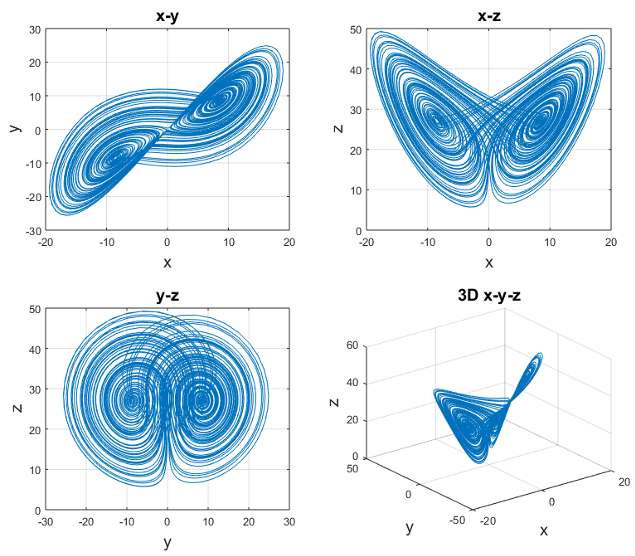
\includegraphics[width=0.9\textwidth]{Immagini/butterfly.png}
\end{figure}    
\end{center}

L'aspetto più sconcertante di questo sistema è la \textbf{dipendenza sensibile dalle condizioni iniziali}: due traiettorie che partono vicinissime l'una all'altra (distanti solo $\delta(0)$) si separano esponenzialmente nel tempo:
\begin{equation}
    ||\delta(t)|| \sim ||\delta(0)|| e^{\lambda t}
\end{equation}
dove $\lambda > 0$ è  \textbf{l'Esponente di Ljapunov}. 

Riassumendo le evidenze emerse da questo sistema, possiamo formulare una definizione pragmatica di \textbf{dinamica caotica}. Diciamo che un sistema esibisce caos se il suo comportamento soddisfa i seguenti tre requisiti:
\begin{enumerate}
    \item L'andamento è \textbf{aperiodico a lungo termine}.
    \item La dinamica è generata da un sistema di equazioni differenziali strettamente \textbf{deterministico} (non ci sono elementi stocastici).
    \item Vi è una \textbf{dipendenza sensibile} dalle condizioni iniziali (manifestata da un esponente di Ljapunov positivo).
\end{enumerate}

\subsection*{Frattali e Dimensione}

Abbiamo stabilito che per $t \to \infty$ le traiettorie dell'attrattore strano si confinano in una regione limitata di volume nullo, pur senza mai chiudersi in orbite periodiche. Per formalizzare la natura geometrica di tali oggetti (che non sono né semplici curve monodimensionali né superfici bidimensionali), occorre introdurre il concetto di \textbf{Frattale}.

Un esempio classico per visualizzare questa anomalia dimensionale è la \textbf{Curva di von Koch}.
Consideriamo un segmento iniziale $S_0$ avente lunghezza $L_0$. L'operazione generatrice (che itereremo all'infinito) consiste in due passaggi:
\begin{enumerate}
    \item Dividere il segmento in 3 parti uguali.
    \item Rimuovere il terzo centrale e sostituirlo con i due lati obliqui di un triangolo equilatero.
\end{enumerate}

\begin{center}
\begin{tikzpicture}[scale=2]
    % S0
    \draw[thick] (0,2) -- (3,2);
    \node[left] at (-0.2, 2) {$S_0$};
    
    % S1
    \draw[thick] (0,1) -- (1,1) -- (1.5, 1.866) -- (2,1) -- (3,1);
    \node[left] at (-0.2, 1) {$S_1$};
    
    % S2
    \draw[thick] 
        (0,0) -- (0.33,0) -- (0.5,0.288) -- (0.66,0) -- (1,0) -- 
        (1.16,0.288) -- (1,0.577) -- (1.33,0.577) -- (1.5,0.866) --
        (1.66,0.577) -- (2,0.577) -- (1.83,0.288) -- (2,0) --
        (2.33,0) -- (2.5,0.288) -- (2.66,0) -- (3,0);
    \node[left] at (-0.2, 0) {$S_2$};
    
    \draw[dashed, ->] (1.5,-0.2) -- (1.5,-0.6);
    \node[below] at (1.5, -0.6) {e continuo indefinitamente...};
\end{tikzpicture}
\end{center}

Chiediamoci ora: l'oggetto limite di questa procedura è una normale curva unidimensionale? 
A ogni iterazione sostituiamo un segmento lungo $\frac{1}{3}L$ con due segmenti di pari lunghezza. Pertanto, la lunghezza totale dell'oggetto aumenta di un fattore $\frac{4}{3}$. Se l'insieme iniziale $S_0$ ha lunghezza $L_0$, avremo:
\begin{equation}
    S_1 \implies L_1 = \frac{4}{3} L_0
\end{equation}
\begin{equation}
    S_n \implies L_n = \left(\frac{4}{3}\right)^n L_0
\end{equation}

Prendendo il limite per infinite iterazioni ($n \to \infty$):
\begin{equation}
    \lim_{n \to \infty} L_n = \lim_{n \to \infty} \left(\frac{4}{3}\right)^n L_0 = \infty
\end{equation}

Giungiamo a una conclusione controintuitiva: la curva limite $S_\infty$ ha una \textbf{lunghezza infinita}, pur rimanendo sempre confinata in una porzione di piano finita. Di conseguenza, la distanza (calcolata seguendo il percorso della curva) tra due punti qualsiasi su di essa diverge anch'essa a infinito.
Questo ci indica che $S_\infty$ non può essere considerata una semplice curva 1D (perché "riempie" lo spazio troppo densamente), pur non possedendo un'area sufficiente a renderla un oggetto 2D. Oggetti geometrici dotati di questa caratteristica sono dotati di una dimensione frazionaria e vengono definiti frattali.

\subsection*{La Box Dimension}
Per caratterizzare formalmente la dimensione di insiemi complessi come i frattali, introduciamo il concetto di \textbf{Box Dimension} (o dimensione scatolare). L'idea di base consiste nel ricoprire l'insieme geometrico in esame con un reticolo di "scatole" (che possono essere segmenti, quadrati o cubi a seconda dello spazio in cui ci troviamo) di lato $\varepsilon$, e contare il numero minimo di scatole $N(\varepsilon)$ necessarie per un ricoprimento completo.

Osserviamo innanzitutto il comportamento di figure geometriche note al variare della risoluzione. Se dimezziamo il lato della scatola (cioè moltiplichiamo la risoluzione per un fattore $r=2$), il numero di scatole $m$ necessarie scala con una potenza dipendente dalla dimensionalità dell'oggetto.

\begin{center}
\begin{tikzpicture}[scale=0.8]
    % Quadrato 1
    \draw[thick] (0,0) rectangle (1.5,1.5);
    \node[below] at (0.75, -0.2) {$r=1 \implies m=1$};

    % Quadrato 2
    \begin{scope}[xshift=4cm]
        \draw[thick] (0,0) rectangle (1.5,1.5);
        \draw (0.75,0) -- (0.75,1.5);
        \draw (0,0.75) -- (1.5,0.75);
        \node[below] at (0.75, -0.2) {$r=2 \implies m=4$};
    \end{scope}

    % Quadrato 3
    \begin{scope}[xshift=8cm]
        \draw[thick] (0,0) rectangle (1.5,1.5);
        \draw (0.5,0) -- (0.5,1.5);
        \draw (1.0,0) -- (1.0,1.5);
        \draw (0,0.5) -- (1.5,0.5);
        \draw (0,1.0) -- (1.5,1.0);
        \node[below] at (0.75, -0.2) {$r=3 \implies m=9$};
    \end{scope}
    
    \node[right, align=left] at (10, 0.75) {Riscalando il lato di un fattore $r$,\\ il numero di scatole necessarie\\ cresce come $m = r^2$ (in 2D).};
\end{tikzpicture}
\end{center}

In generale, per scatole di lato $\varepsilon$:
\begin{itemize}
    \item Per una \textbf{curva} unidimensionale di lunghezza $L$: il numero di scatole necessarie è proporzionale a $N(\varepsilon) \sim \frac{L}{\varepsilon} \sim \frac{1}{\varepsilon^1}$.
    \item Per una \textbf{superficie} bidimensionale di area $A$: il numero di scatole necessarie è proporzionale a $N(\varepsilon) \sim \frac{A}{\varepsilon^2} \sim \frac{1}{\varepsilon^2}$.
\end{itemize}

\begin{tikzpicture}[scale=1.2, >=stealth]

    % ==========================================
    % GRAFICO 1: Curva unidimensionale (Sinistra)
    % ==========================================
    \begin{scope}[xshift=0cm, yshift=0.75cm] % yshift per allinearlo visivamente all'altro
        
        % Disegna la griglia (le scatole)
        \draw[step=0.5cm, draw=gray, thin] (0,0) grid (4, 0.5);
        
        % Disegna la curva
        % Usiamo bezier (controls) per fare una curva morbida simile all'esempio
        \draw[thick, blue] (0, 0.25) 
              .. controls (0.5, 0.8) and (1.2, -0.2) .. (2, 0.1) 
              .. controls (3, 0.5) and (3.5, 0.1) .. (4, 0.4);
              
        % Etichetta sotto il grafico
        \node at (2, -0.8) {$N(\varepsilon) \sim \frac{L}{\varepsilon}$};
        
    \end{scope}

    % ==========================================
    % GRAFICO 2: Superficie bidimensionale (Destra)
    % ==========================================
    \begin{scope}[xshift=6cm]
        
        % Colora l'interno dell'ellisse (sfondo azzurro chiaro)
        % Lo facciamo prima della griglia così la griglia ci passa sopra
        \fill[blue!15] (2.25, 1) ellipse (1.8cm and 0.9cm);
        
        % Disegna la griglia (le scatole)
        \draw[step=0.5cm, draw=gray, thin] (0,0) grid (4.5, 2);
        
        % Disegna il contorno dell'ellisse sopra la griglia
        \draw[thick, blue] (2.25, 1) ellipse (1.8cm and 0.9cm);
        
        % Etichetta sotto il grafico
        \node at (2.25, -0.5) {$N(\varepsilon) \sim \frac{A}{\varepsilon^2}$};
        
    \end{scope}

\end{tikzpicture}


Generalizzando questo concetto, per un insieme $D$-dimensionale ci aspettiamo un asintotico andamento del tipo $N(\varepsilon) \sim \frac{1}{\varepsilon^d}$. Invertendo questa relazione per isolare l'esponente, si giunge alla definizione formale di \textbf{Box Dimension} $d$:
\begin{equation}
    d = \lim_{\varepsilon \to 0} \frac{\ln N(\varepsilon)}{\ln \left(\frac{1}{\varepsilon}\right)}
\end{equation}

\subsubsection*{Esempio: L'insieme di Cantor}
Un esempio emblematico per il calcolo della dimensione frattale è l'\textbf{insieme di Cantor}. Questo si costruisce partendo da un segmento unitario $[0,1]$ e rimuovendo iterativamente, a ogni passo, il terzo centrale di ciascun sotto-intervallo rimanente.

Al passo $m$-esimo, l'insieme $S_m$ è costituito da $2^m$ intervallini, ciascuno avente una lunghezza pari a $\left(\frac{1}{3}\right)^m$. 
Per calcolarne la dimensione, scegliamo di utilizzare "scatole" unidimensionali di lunghezza esattamente pari agli intervallini, ponendo $\varepsilon = \left(\frac{1}{3}\right)^m$. Notiamo che per $m \to \infty$, coerentemente con la definizione, si ha $\varepsilon \to 0$. Per coprire $S_m$, avremo bisogno esattamente di $N(\varepsilon) = 2^m$ scatole. Sostituendo nella definizione di Box Dimension, troviamo:
\begin{equation}
    d = \lim_{m \to \infty} \frac{\ln(2^m)}{\ln\left( \frac{1}{(1/3)^m} \right)} = \lim_{m \to \infty} \frac{m \ln 2}{m \ln 3} = \frac{\ln 2}{\ln 3} \simeq 0.63
\end{equation}
L'insieme di Cantor possiede una dimensione frazionaria (compresa tra 0 e 1). Questa estensione della nozione matematica di dimensione risulta particolarmente utile in quanto permette di caratterizzare quantitativamente la densità di insiemi rarefatti, o l'irregolarità di curve continue ma non differenziabili.


\subsection*{Mappa del Panettiere e Attrattori Strani}

Siamo ora in grado di comprendere l'origine della complessa struttura geometrica degli attrattori caotici. Ci chiediamo: in che modo le traiettorie di un sistema dissipativo possono separarsi in modo esponenziale (dimostrando dipendenza sensibile dalle condizioni iniziali) ed essere allo stesso tempo confinate perpetuamente all'interno di una regione compatta e finita dello spazio delle fasi?

\subsubsection*{Il Meccanismo di Stretching and Folding}
Intuitivamente, la risposta risiede nel meccanismo topologico di \textbf{stretching and folding} (stiramento e ripiegamento) dello spazio delle fasi. Immaginiamo l'atto di impastare la pasta: tiriamo la massa in una direzione (allontanando esponenzialmente due particelle originariamente vicine) e successivamente la ripieghiamo su sé stessa (assicurando che la massa rimanga confinata in un volume finito). Se deponessimo due minuscole gocce di colorante vicinissime nell'impasto, dopo un elevato numero di iterazioni di questo processo, i due colori verrebbero inesorabilmente separati e ridistribuiti ovunque, delineando l'incertezza e la mescolanza tipiche del caos.

\begin{center}
\begin{tikzpicture}[
    >=Latex,
    % Stili
    phasebox/.style={draw=gray!80, dashed, thick, rounded corners=3pt, fill=blue!2},
    dough/.style={fill=orange!30, draw=orange!80!black, thick},
    dotred/.style={circle, fill=red, inner sep=1.8pt, draw=black, very thin},
    dotblue/.style={circle, fill=blue!80!black, inner sep=1.8pt, draw=black, very thin},
    arrow/.style={->, very thick, color=black!70},
    textlabel/.style={align=center, font=\footnotesize, text=black!80}
]

    % TITOLO DEL GRAFICO
    \node[font=\large\bfseries, text=black!80] at (4, 3) {Il Meccanismo di Stretching \& Folding};

    % ==========================================
    % STADIO 1: CONDIZIONI INIZIALI
    % ==========================================
    \begin{scope}[shift={(0,0)}]
        % Spazio delle fasi compatto
        \draw[phasebox] (-1.5, -1.5) rectangle (1.5, 1.5);
        
        % Blob di pasta (Stato iniziale)
        \filldraw[dough] (0,0) circle (1.2);
        
        % Punti (Gocce di colorante)
        \node[dotred] (R1) at (-0.1, 0) {};
        \node[dotblue] (B1) at (0.1, 0) {};
        
        % Etichette
        \node[textlabel] at (0, -2) {\textbf{1. Stato Iniziale}\\Spazio delle fasi compatto.\\Due punti molto vicini.};
    \end{scope}

    % FRECCIA 1 -> 2 (Stiramento)
    \draw[arrow] (1.8, 0) -- (3.5, 0) node[midway, above, font=\footnotesize\bfseries] {Stiramento};

    % ==========================================
    % STADIO 2: STRETCHING
    % ==========================================
    \begin{scope}[shift={(8,0)}]
        % Lo spazio originale per far vedere che esce dai bordi prima del ripiegamento
        \draw[phasebox] (-1.5, -1.5) rectangle (1.5, 1.5);
        
        % Blob stirato
        \filldraw[dough, rounded corners=6pt] (-2.8, -0.3) rectangle (2.8, 0.3);
        
        % Punti allontanati
        \node[dotred] (R2) at (-2.2, 0) {};
        \node[dotblue] (B2) at (2.2, 0) {};
        
        % Etichette
        \node[textlabel] at (0, -2) {\textbf{2. Stretching}\\I punti si separano\\esponenzialmente.};
    \end{scope}

    % FRECCIA 2 -> 3 (Ripiegamento)
    \draw[arrow] (7, -2.5) to[out=240, in=30] (5.5, -4) node[midway, right=0.1cm, font=\footnotesize\bfseries] {Ripiegamento};

    % ==========================================
    % STADIO 3: FOLDING
    % ==========================================
    \begin{scope}[shift={(4,-6)}]
        % Spazio delle fasi (confinamento)
        \draw[phasebox] (-1.5, -1.5) rectangle (1.5, 1.5);
        
        % Ferro di cavallo (Blob ripiegato)
        % Matematicamente costruito per essere uno spessore uniforme
        \filldraw[dough] 
            (-1.1, -0.8) -- (-1.1, 0.2) arc (180:0:1.1) 
            -- (1.1, -0.8) arc (360:180:0.3) 
            -- (0.5, 0.2) arc (0:180:0.5) 
            -- (-0.5, -0.8) arc (360:180:0.3) -- cycle;
            
        % Punti ora lontani lungo la massa, ma dentro lo stesso volume
        \node[dotred] (R3) at (-0.8, -0.3) {};
        \node[dotblue] (B3) at (0.8, -0.3) {};
        
        % Etichette
        \node[textlabel] at (0, -2.2) {\textbf{3. Folding}\\Il sistema è ripiegato su sé stesso.\\La massa rimane confinata\\nel volume originario.};
    \end{scope}

    % FRECCIA 3 -> 1 (Iterazione / Caos)
    \draw[arrow] (2.2, -4.5) to[out=135, in=300] (0.5, -2.8) node[midway, left=0.1cm, font=\footnotesize\bfseries] {Re-iterazione};

\end{tikzpicture}
\end{center}

\subsubsection*{La Mappa del Panettiere}
Un modello matematico rigoroso che implementa esplicitamente questo comportamento è la \textbf{Mappa del Panettiere} (Baker's Map), una trasformazione discreta del quadrato unitario $[0,1] \times[0,1]$ in sé stesso. Definiamo un parametro $a \in \left(0, \frac{1}{2}\right]$ che rappresenta la contrazione verticale. La mappa è definita a tratti come:
\begin{equation}
    (x_{n+1}, y_{n+1}) = 
    \begin{cases} 
        (2x_n, a y_n) & 0 \leq x_n \leq \frac{1}{2} \\ 
        (2x_n - 1, a y_n + \frac{1}{2}) & \frac{1}{2} < x_n \leq 1 
    \end{cases}
\end{equation}

\subsubsection*{Interpretazione Geometrica dell'Azione}
L'azione della mappa su un insieme di condizioni iniziali disposte sul quadrato di lato 1 si articola in due passaggi distinti:
\begin{enumerate}
    \item \textbf{Stretching e Contrazione:} La coordinata $x$ viene moltiplicata per 2, originando uno stiramento orizzontale responsabile della separazione esponenziale delle traiettorie. Contemporaneamente, la coordinata $y$ subisce una contrazione verticale dettata dal fattore $a \le \frac{1}{2}$.
    \item \textbf{Taglio e Riposizionamento:} Applicando il primo passaggio, la metà destra dell'insieme cadrebbe fuori dal dominio originario (avendo $x > 1$). Il termine $-1$ sulla coordinata $x$ e il termine $+\frac{1}{2}$ sulla coordinata $y$ corrispondono all'operazione di taglio della porzione "eccedente" e al suo riposizionamento al di sopra della metà sinistra, attuando così il "ripiegamento" all'interno del quadrato originale.
\end{enumerate}

\begin{center}
\begin{tikzpicture}[scale=2.5]
    % 1. Quadrato Iniziale
    \draw[thick] (0,0) rectangle (1,1);
    \draw[dashed, red] (0.5,0) -- (0.5,1); % Linea di taglio
    
    % Faccina
    \draw[red, thick] (0.5, 0.5) circle (0.3);
    \filldraw[red] (0.4, 0.6) circle (0.03);
    \filldraw[red] (0.6, 0.6) circle (0.03);
    \draw[red, thick] (0.35, 0.4) arc (200:340:0.15);
    \node[below] at (0.5, -0.1) {Cond. Iniziale $S$};

    % Freccia 1
    \draw[->, thick] (1.2, 0.5) -- (1.6, 0.5) node[midway, above, font=\footnotesize] {Stretching $x \times 2$} node[midway, below, font=\footnotesize] {Contrazione $y \times a$};

    % 2. Rettangolo stirato
    \begin{scope}[xshift=1.8cm, yshift=0.35cm]
        \draw[thick] (0,0) rectangle (2,0.3);
        \draw[dashed, red] (1,0) -- (1,0.3); % Linea di taglio
        
        % Faccina deformata
        \draw[red, thick] (1, 0.15) ellipse (0.6 and 0.09);
        \filldraw[red] (0.8, 0.18) circle (0.02 and 0.01);
        \filldraw[red] (1.2, 0.18) circle (0.02 and 0.01);
        \draw[red, thick] (0.7, 0.12) arc (200:340:0.3 and 0.045);
    \end{scope}

    % Freccia 2
    \draw[->, thick] (4.0, 0.5) -- (4.4, 0.5) node[midway, above, font=\footnotesize] {Taglio e} node[midway, below, font=\footnotesize] {Shift};

    % 3. Immagine finale
    \begin{scope}[xshift=4.6cm]
        \draw[thick] (0,0) rectangle (1,1);
        
        % Striscia bassa (sinistra dell'immagine stirata)
        \draw[fill=blue!10, thick] (0,0) rectangle (1,0.3);
        % Mezza faccia sinistra
        \clip (0,0) rectangle (1,0.3);
        \draw[red, thick] (1, 0.15) ellipse (0.6 and 0.09);
        \filldraw[red] (0.8, 0.18) circle (0.02 and 0.01);
        \draw[red, thick] (0.7, 0.12) arc (200:340:0.3 and 0.045);
    \end{scope}
    \begin{scope}[xshift=4.6cm]
        % Striscia alta (destra dell'immagine stirata)
        \draw[fill=blue!10, thick] (0,0.5) rectangle (1,0.8);
        \clip (0,0.5) rectangle (1,0.8);
        \draw[red, thick] (0, 0.65) ellipse (0.6 and 0.09);
        \filldraw[red] (0.2, 0.68) circle (0.02 and 0.01);
        \draw[red, thick] (-0.3, 0.62) arc (200:340:0.3 and 0.045);
    \end{scope}
    \node[below] at (5.1, -0.1) {Mappa $B(S)$};

\end{tikzpicture}
\end{center}

Se applichiamo ripetutamente la mappa sul quadrato iniziale $S$, si forma una caratteristica geometria a strisce la cui granularità decresce iterazione dopo iterazione:
\begin{itemize}
    \item $S$ è un quadrato unico di lato 1.
    \item L'immagine $B(S)$ è formata da $2$ strisce orizzontali di altezza $a$.
    \item L'immagine successiva $B^2(S)$ è composta da $4$ strisce di altezza $a^2$.
    \item Al passo $n$-esimo, $B^n(S)$ presenterà esattamente $2^n$ strisce di altezza $a^n$.
\end{itemize}

\begin{center}
\begin{tikzpicture}[scale=1.5]
    % S
    \draw[thick] (0,0) rectangle (1,1);
    \node[below] at (0.5,0) {$S$};
    
    \draw[->, thick] (1.2,0.5) -- (1.5,0.5);

    % B(S)
    \begin{scope}[xshift=1.7cm]
        \draw[thick] (0,0) rectangle (1,1);
        \draw[fill=blue!30] (0,0) rectangle (1,0.2);
        \draw[fill=blue!30] (0,0.5) rectangle (1,0.7);
        \node[below] at (0.5,0) {$B(S)$};
    \end{scope}

    \draw[->, thick] (2.9,0.5) -- (3.2,0.5);

    % B^2(S)
    \begin{scope}[xshift=3.4cm]
        \draw[thick] (0,0) rectangle (1,1);
        \draw[fill=blue!50] (0,0) rectangle (1,0.05);
        \draw[fill=blue!50] (0,0.25) rectangle (1,0.3);
        \draw[fill=blue!50] (0,0.5) rectangle (1,0.55);
        \draw[fill=blue!50] (0,0.75) rectangle (1,0.8);
        \node[below] at (0.5,0) {$B^2(S)$};
    \end{scope}
\end{tikzpicture}
\end{center}

\subsubsection*{Calcolo della Dimensione dell'Attrattore $B^\infty(S)$}
Dato che per la struttura stessa della trasformazione vale $B^{n+1}(S) \subset B^n(S)$, l'insieme limite per $n \to \infty$ è l'intersezione di una successione di compatti incapsulati ed è, quindi, un insieme non vuoto. Definiamo questo limite come $A = B^\infty(S)$. Ogni condizione iniziale posta all'interno di $S$ tenderà asintoticamente verso questo insieme, che prende il nome di \textbf{attrattore}.

Possiamo derivare la Box Dimension dell'attrattore $A$ assumendo $a < \frac{1}{2}$. Adoperiamo un reticolo formato da scatole di lato $\varepsilon = a^n$ per ricoprire l'approssimazione $B^n(S)$. Dal momento che una singola striscia si estende in larghezza per tutto il dominio $x \in [0,1]$, saranno necessarie $1/a^n$ scatole adiacenti per coprirne la lunghezza. Avendo in totale $2^n$ strisce indipendenti, il numero di scatole minime necessarie sarà:
\begin{equation}
    N(\varepsilon) \sim \frac{1}{a^n} \times 2^n = \left(\frac{a}{2}\right)^{-n}
\end{equation}
Applicando la definizione di Box Dimension per $n \to \infty$ (che implica $\varepsilon \to 0$):
\begin{equation}
    d = \lim_{n \to \infty} \frac{\ln\left[ \left(\frac{a}{2}\right)^{-n} \right]}{\ln(1/a^n)} = \lim_{n \to \infty} \frac{-n \ln(a/2)}{-n \ln a} = \frac{\ln a - \ln 2}{\ln a} = 1 - \frac{\ln 2}{\ln a} = 1 + \frac{\ln(1/2)}{\ln a}
\end{equation}

Questo importante risultato porta a due considerazioni chiave a seconda del parametro di contrazione $a$:
\begin{itemize}
    \item Nel caso limite in cui $a = \frac{1}{2}$, si ottiene $d = 1 - \frac{\ln 2}{\ln(1/2)} = 1 - (-1) = 2$. Dal punto di vista dinamico, la mappa preserva le aree ad ogni iterazione, la dinamica è puramente conservativa, e l'attrattore riempie interamente e uniformemente lo spazio.
    \item Quando $a < \frac{1}{2}$, il sistema diventa globalmente dissipativo in quanto le aree nel piano vengono contratte strettamente ($\text{Area}(B(R)) < \text{Area}(R)$). La dimensione ottenuta $d$ risulta essere un numero frazionario. L'attrattore ha misura di Lebesgue (area) nulla, seppur attraendo un bacino aperto di condizioni iniziali. Un siffatto insieme, invariante ma contraddistinto da topologia complessa e dimensione frattale, è un autentico \textbf{Attrattore Strano}.
\end{itemize}



\end{document}
